%!TEX program=lualatex
\documentclass[finemath,svgnames,twoside,chapter,no-math]{oblivoir}
    %\usepackage{processdata,ikpscon,indentfirst,makeidx} 
    \usepackage[kopub,print]{OVERTHECON}
    
    \usepackage{intothemath,memtikzpagenodes,indentfirst,makeidx,kswrapfig} 
    \usepackage{rotating}
    \usepackage{multicol}
      \usepackage[level=part]{obchaptertoc}
      \chaptertocmaxlevel{section} \renewcommand\chaptertocfont{\normalfont\normalsize\selectfont} \renewcommand\printparttitle[1]{#1\par\vspace{40pt}\chaptertoc}
       % \TOCFormatsamsas{subsection}{section}{dotsep,presnum}

  %%

    \newcommand{\nosol}{해설없음}
    %\usepackage{enumitem}
    %\usepackage{dhucs-enumitem}
    %\setlist{  
    %  listparindent=\parindent,     
    %  parsep=0pt,   
    %}         
                  \renewcommand{\thefootnote}{\:\color{cyan}(\arabic{footnote})}
    \usepackage{newbox}     
           \usepackage{slashbox}
    \trimLmarks
    \newcommand\answerTableNum[1]{%
    \cellcolor{gray!20}%
    \textbf{\color{cyan!100}#1}%
    }
    
    \newcommand\answerTableTitle[1]{%
    \cellcolor{black!60}%
    \textbf{\color{white}\LARGE#1}%
    }

\makeatletter
\patchcmd
	\tabu@startpboxmeasure
	{\bgroup\begin{varwidth}}%
	{\bgroup
	 \iftabu@spread\color@begingroup\fi\begin{varwidth}}%
	{}{}
\def\@tabarray{\m@th\def\tabu@currentgrouptype
    {\currentgrouptype}\@ifnextchar[\@array{\@array[c]}}
%
%%% \pdfelapsedtime bug 2019-12-15
\patchcmd
	\tabu@message@etime
	{\the\pdfelapsedtime}%
	{\pdfelapsedtime}%
	{}{}
%
%


\makeatother
%\renewcommand\booktitlehead{}
\renewcommand\hparttitlehead{}
\renewcommand\hchaptertitlehead{\parttitle\thepart.\thechapter)}
\newcommand{\parttitle}{}
% -----------------------------


%%%%%%%%%%%%%%%%%%%%
\SetValue{conpicsize}{0.15}
\SetValue{solpicsize}{0.125}
\SetValue{picsize}{0.125}
\SetValue{Cansu}{2}
\gdef\mytmplist{}
\foreach \i in {1,...,\pgfkeysvalueof{Cansu}}%
    {%
        \xdef\mytmplist{\mytmplist ../}%
    }%
\xdef\mytmplist{\mytmplist Problems/DBs/}
\SetValue{problemPath}{\mytmplist}
\newcommand{\mygachapter}{\chapter}


\newenvironment{exercise}
{%before
\refstepcounter{exercise}%
\ifthenelse{\equal{\GetValue{type}}{solution}}
  {%true
  \ifthenelse{\equal{\GetValue{HOFMode}}{on}}
    {%true
    }{%false
    \noindent{\Huge\myCentury\ifnum\value{exercise}<10{\color{cyan!50}0}\fi\color{cyan}\arabic{exercise}}\enspace
    }%
  }{%false
  \ifthenelse{\equal{\GetValue{HOFMode}}{on}}
    {%true
    }{%false
    \noindent{\Huge\myCentury\ifnum\value{exercise}<10{\color{cyan!50}0}\fi\color{cyan}\arabic{exercise}}\enspace
    }%
  }%
}{%after
\par\vskip 2\baselineskip minus 1.5\baselineskip}


%%%%%%%%%%%%%%%%%%%%
\SetValue{conpicsize}{0.15}
\SetValue{solpicsize}{0.125}
\SetValue{picsize}{0.125}
%%%%%%%%%%%%%%%%%%%%
 \makeindex   
 
 
%\titlespacing*{\part}
%  {0pt}{50pt}{40pt}
%\titlespacing*{\chapter}
%  {0pt}{0pt}{20pt}
\renewcommand\cftbooknumwidth{0.0em}
\renewcommand\cftpartindent{0.2em}
\renewcommand\cftpartnumwidth{0.7em}
\renewcommand\cftchapterindent{1.5em}
\renewcommand\cftchapternumwidth{7.0em}

\renewcommand{\cftbookfont}{\bfseries\sffamily}
\renewcommand{\cftpartfont}{\bfseries\sffamily}
\renewcommand{\cftchapterfont}{\sffamily}
\renewcommand*{\cftbookpagefont}{\bfseries\sffamily}
\renewcommand*{\cftpartpagefont}{\bfseries\sffamily}
\renewcommand*{\cftchapterpagefont}{\sffamily}
\counterwithin*{chapter}{part}
\setcounter{tocdepth}{1}

\ChapterTOCFormat{%
\renewcommand\cftchapterindent{0.0em}
\renewcommand\cftsectionindent{3.0em}
\renewcommand\cftchapternumwidth{7.0em}
\renewcommand\cftsectionnumwidth{7.0em}
\renewcommand\cftsectionfont{\sffamily\small}
\renewcommand*{\cftsectionpagefont}{\sffamily}
}
%\doparttoc% Prepare minitoc package for part tocs usage
\begin{document} 

\chapterstyle{my}
\setsecnumdepth{chapter}
\SetValue{type}{problem}
\renewcommand{\thepart}{\arabic{part}}
\renewcommand{\thebook}{}
\pagestyle{empty}
타이틀링페이지(내부표지들어갈자리)
\newpage
\pagestyle{overthecon}
저자정보들어갈자리
\clearpage

\setsecnumdepth{chapter}\setcounter{chapter}{-1}\renewcommand{\parttitle}{Intro }

\pagestyle{overthecon}
\mychapter{교재 구성 및 활용법}{}

\section{교재 소개 : 단원을 넘나들며 함수를 중심으로 학습하는 전범위 통합개념서}
이 책의 제목은 \cnm{인투더 수학 I \& II}이지만, 사실 더 적합한 제목은 \cnm{인투더 함수}라 할 수 있을 정도로, 모든 내용은 함수를 중심으로 편성되어 있습니다. 고등학교 1학년 \cnm{수학}은 모두 함수를 다루기 위한 재료들을 준비하는 단계이고, \cnm{수학 I}은 새로운 함수들을 배우는 과목이며, \cnm{수학 II}는 익숙한 함수였던 다항함수를 미적분이라는 도구를 이용하여 분석하는 과목이기 때문입니다. 즉 \cnm{수학 I}과 \cnm{수학 II}의 전범위 개념을 완전히 장악하기 위해서는 그 공통분모인 함수에 대한 개념을 정확히 확립해야 한다고 볼 수 있습니다.

대부분의 다른 수학 개념 교재들은 물론이고, 인투더 시리즈의 다른 책들인 \cnm{인투더 중학도형}, \cnm{인투더 확률과 통계}, \cnm{인투더 기하}, \cnm{인투더 미적분}도 대체로 단원순서대로 공부하는 구성을 따르고 있습니다. 이에 반해 \cnm{인투더 수학 I \& II}는 \cnm{수학}, \cnm{수학 I}, \cnm{수학 II}를 넘나들며 함께 다룰 수 있는 주제들을 묶어가며 가르칩니다. 통합수능 체제에서 \cnm{수학 I}과 \cnm{수학 II}가 통합된 문제를 출제하며 수험생들에게 한 단원에 갇힌 좁은 시야에서 벗어나기를 요구한다는 점에서, 이러한 구성의 교재를 학습하는 것은 여러분께 넓게 바라보는 안목을 갖출 수 있도록 도울 것입니다.
\section{교재 구성}
이 책은 다음과 같이 구성되어 있습니다. 
\begin{itemize}
    \item Zero : \cnm{수학}, \cnm{수학 I}, \cnm{수학 II}의 기본 용어
    \item Graph : 함수의 그래프와 관련된 개념의 시각화
    \item Basic : Zero와 Graph의 내용을 수식으로 엄밀화
    \item Algebra : 2015 개정 교육과정 수학 I (2022 개정 교육과정 대수-Algebra)
    \item Calculus : 2015 개정 교육과정 수학 II (2022 개정 교육과정 미적분 I-Calculus)
\end{itemize}
뒷 단원은 앞 단원의 내용을 숙지했다는 전제 하에 내용이 구성되어 있습니다. 따라서 뒷 단원을 먼저 읽는 것은 권장하지 않습니다. 


%용어 파트와 원리 파트를 공부함으로써, 쎈수학 A단계와 B단계 난이도(하), 교과서 본문에 제시되는 예제와 유제 수준, 수능에서는 모든 2점 문항과 쉬운 3점 문항을 스스로 풀이할 기초를 닦을 수 있습니다.

%이해 파트를 공부함으로써, 쎈수학 B단계 난이도(중), 교과서 단원 후반에 제시되는 문항 수준, 수능에서는 일반적인 3점 문항과 쉬운 4점 문항을 풀이하는 데 필요한 소양을 갖출 수 있습니다.

%응용파트를 공부함으로써, 쎈수학 B단계 난이도(중, 상)과 C단계, 교과서에 실린 고난도 문항이나 수능 4점 문항에 대응할 준비를 마칠 수 있습니다.

\section{교재 활용법 : 다회독을 통한 개념 구조의 확립}
뒤이어 설명할 단원별 공부법을 참고하여 1회독을 마친 뒤, 2회독부터는 1회독에서 이미 알고 있던 내용이나 쉽다고 느꼈던 부분을 건너뛰며 학습합니다. 익숙하지 않았거나 완전히 이해되지 않은 부분만 집중적으로 학습하며 약점을 메웁니다. 회독을 거듭할 수록, 교육과정 전반에서 다루는 함수의 기초부터 핵심까지 뚜렷한 이미지를 확립할 수 있을 것입니다.

\section{단원별 공부법}

\subsection{Zero : 가능한 빠르게 읽고, 빈 부분이 있다면 체크하자}
Zero는 본 교재를 공부하기 위해 꼭 알고 있어야 하는 교과서 기본 개념을 담고 있습니다. 단순히 교육과정 순서대로 나열한 것이 아니라, 기본개념을 한 번 이상 공부한 학생이 12년치의 교과 개념을 가장 빠르고 효율적으로 재확인할 수 있도록 최적화하였습니다.

Zero를 읽어나가면서 의구심이 들거나 알 듯 말 듯 애매한 개념들이 있는지를 확인해야 합니다. 그런 게 없다면 개념이 탄탄함을 확인해서 좋은 것이고, 있다면 이를 보완할 수 있게 되어 다행이라고 생각합시다. 단, Zero에서 저자의 판단에 따라 상세한 설명이나 증명을 제시하는게 필요한 경우에는 제시되어 있지만, 대부분의 경우는 증명이나 상세한 설명이 없습니다. 그러한 경우에는 교과서나 참고서를 활용하여 해당 내용을 확인하여 개념을 보완하시기 바랍니다.

학생에 따라서는 어차피 쉬운 개념이고 단순한 나열인데 Zero 공부 안하고 뛰어넘으면 안되냐고 생각할 수 있겠습니다. 그러나 교과서에서는 본 적이 없는 서술, 표현, 용어 등이 약간씩 들어있으므로, 원활한 학습을 위해서는 Zero를 꼭 공부해야 합니다.  또한 이 책의 본문은 Zero를 다 읽었다는 전제 하에 서술되므로, 이 책을 효과적으로 공부하기 위해서는 Zero를 반드시 학습하기를 권합니다.

\subsection{Graph : 개념의 정의를 암기하고, 정의에서 파생된 성질을 시각화한 내용에 익숙해지자}
함수는 수식으로 다루는 것도 중요하지만, 그래프를 통해 시각화된 내용에 친숙해야 합니다. 이는 수능이 엄밀성을 요구하는 서술형 시험이 아닌, 직관과 비약을 어느 정도 허용하는 단답형 시험이기 때문에 더욱 그렇습니다. 이를 위해 Graph에서는 함수와 관련된 여러 가지 정의와 성질들을 알려주고, 정의와 성질로부터 끌어낼 수 있는 여러 상황들을 증명 없이 제시합니다. 따라서 각 정의를 확실히 암기하고, 성질을 이해하고, 시각화된 결과물들에 친숙해지는 것이 필요합니다. \clearpage

\subsection{Basic : 함수의 엄밀화}
Basic은 Zero와 Graph까지만 알고 있는 상황에서 본격적인 함수 분석을 다루기 전 이야기할 수 있는 함수 관련 내용을 주제별로 엮어 배웁니다. Basic을 배울 때에는 앞서 배운 내용들이 계속 복선처럼 활용되므로, 반복 학습을 통해 익숙해질 수 있도록 도와줍니다.

\subsubsection{Basic 1) 수식으로 다루는 함수의 성질}
지금까지 배운 내용을 수식으로 검증하는 단원입니다. 아무리 수능이 직관적이거나 감각적인 영역이 강조된다고 하더라도, 수식을 아예 배제할 수는 없습니다. 그래서 Graph로 여러 정의와 성질에 익숙해졌다면, 이제 수식과 논리로 바탕을 든든히 해야 할 것입니다. Basic 1)을 통해 Graph에서 배운 내용을 더 깊이 이해할 수 있고, 확실하게 익숙해질 수 있을 것입니다. 수식 활용 능력과 논리를 익히는 건 보너스입니다.


\subsubsection{Basic 2) 점근선과 극한의 논리 완성}
어물쩡 대충 계산하고 넘어가는 극한이 아닌, 논리에 근거해 깔끔하게 풀이하는 극한을 배웁니다. `대충 뭐가 어디로 가고 어디로 가니까 뭐가 어떻고$\cdots$'와 같이 확실하지 않은 애매한 풀이를 해왔다면, 이 중단원을 통해 논리적으로 극한을 풀이할 수 있을 것입니다.

\subsubsection{Basic 3) 여러 가지 함수의 분석}
교육과정 순서대로 각 함수의 특징을 되돌아봅니다. 또한 지금까지 배운 내용을 바탕으로 다항함수를 두 소단원에 걸쳐 분석하면서 다항함수에 대해 더 깊게 이해할 수 있습니다.

\subsection{Algebra : 더 많은 함수들과 함수로서의 수열(수학 I)}
Algebra에서는 지금까지 다룬 내용들을 바탕으로 \cnm{수학 I}을 다시 살펴봅니다. 많은 내용들을 알게 모르게 앞에서 다루어왔으므로, Algebra 단원에서는 쉬어간다는 느낌으로 앞에서 배운 내용들을 언급하며 가볍게 개념들을 리마인드하고, 각 개념에 대해 새롭게 해석하는 관점들을 제공합니다.


\subsection{Calculus : 미적분을 통한 다항함수의 분석과 합성함수 특강(수학 II)}
지금까지 배운 내용을 모두 종합하여 다항함수의 미적분을 완성하고, 미처 다루지 못한 미분계수, 적분의 의미, 수직선에서의 물리학을 다룹니다. 마지막으로 미적분 미선택자의 불리함을 완화하는 특강으로 마무리짓습니다.


\begin{comment}
\section{1권 : 문제는 거들 뿐, 이론 확립을 위해 개념 위주로 학습합니다.}
이 책은 수능에 필요한 대부분의 미적분 이론을 한 권에 꾹꾹 눌러담는 것을 목표로 했기 때문에, 1권 본문에는 일부 예외적인 경우를 제외하고는 수록된 문제가 없습니다. 이 책의 예상 독자가 `미적분 전범위를 어느 정도 공부한 경험이 있는 상태에서 개념을 체계적으로 정립하려는 학생'이므로, 수록된 문제가 많지 않다는 것만 미리 알고 있으면 학습에 큰 지장이 없을 것입니다.

\section{2권 : 2005\anfruf2011 \cnm{미적분} 기출문제로 문제풀이에 적용하세요.}
1권에는 개념만 있고 문제풀이가 없는데 1권만 공부하면 개념이 탄탄해졌으니 수능 점수가 잘 나오느냐? 그것은 아닙니다. 1권에서 배운 이론을 기출문제에 실제로 사용해보고 정말 내가 이론을 잘 알고 있는지, 문제풀이에는 잘 적용할 수 있는지 확인하고 연습해야겠죠. 

이는 2권에서 다룹니다. 1권의 내용을 바탕으로, 2005학년도\textasciitilde{}2011학년도의 평가원/수능 \cnm{미적분} 주요 기출문제들을 연도순서대로 분석합니다. 수능이론의 내용이 기출문제에 어떻게 접목되는지를 설명함과 동시에, 일관성을 유지하면서도 꾸준히 변형/발전하는 기출문제의 출제 경향을 생생하게 배울 수 있을 것입니다.

2005\anfruf{}2011 \cnm{미적분} 기출문제 중 빠진 문항들과 2012\anfruf{}2021학년도의 \cnm{미적분} 평가원/수능 기출문제들은 12월에 출간될 \cnm{트리플기출}에서 다룹니다. 특수주제 문항(극한-도형 응용, 변화율 등)을 제외하고는 2권과 마찬가지로 연도순서대로 분석하므로 일관적인 기출 학습이 가능할 것입니다.


\mychapter{단원별 공부법}{}
\section{단원별 명명법}
단원의 이름을 부르는 법부터 약속합시다. 단원은 대중소로 나뉘는데, 대단원은 Zero, Integral, Function, Limit, Special의 5개로 나뉩니다. Limit 1)과 Function 3)은 중단원을 부르는 이름입니다. Zero 2.1)과 Special 3.2)는 소단원을 부르는 이름입니다.

\section{Zero : 가능한 빠르게 읽고, 빈 부분이 있다면 체크하자}
Zero는 본 교재를 공부하기 위해 꼭 알고 있어야 하는 \cnm{미적분}의 교과서 기본 개념을 담고 있습니다. Zero를 읽어나가면서 의구심이 들거나 알 듯 말 듯 애매한 개념들이 있는지를 확인해야 합니다. 그런 게 없다면 개념이 탄탄함을 확인해서 좋은 것이고, 있다면 이를 보완할 수 있게 되어 다행이라고 생각합시다. 단, Zero에서 저자의 판단에 따라 상세한 설명이나 증명을 제시하는게 필요한 경우에는 제시되어 있지만, 대부분의 경우는 증명이나 상세한 설명이 없습니다. 그러한 경우에는 교과서나 참고서를 활용하여 해당 내용을 확인하여 개념을 보완하시기 바랍니다.

학생에 따라서는 어차피 쉬운 개념이고 단순한 나열인데 Zero 공부 안하고 뛰어넘으면 안되냐고 생각할 수 있겠습니다. 그러나 교과서에서는 본 적이 없는 서술, 표현, 용어 등이 들어있으므로, 원활한 학습을 위해서는 Zero를 꼭 공부해야 합니다.  또한 이 책의 본문은 Zero를 다 읽었다는 전제 하에 서술되므로, 이 책을 효과적으로 공부하기 위해서는 Zero를 반드시 학습하기를 권합니다.

\section{Integral : 적분 테크닉의 연마}
\cnm{수학 II}의 적분과 \cnm{미적분}의 적분의 가장 두드러진 차이점은 함수를 적분하는 데 여러 테크닉이 필요하다는 점입니다. 본질을 잊지 않은 채 각 테크닉을 배워나갈 수 있도록 합니다.

\subsection{Integral 1) 기본적인 적분 테크닉}
단순히 Case by case식의 접근이 아닌, 각 테크닉의 본질적 요소를 탐구하여 적분 테크닉의 기본기를 탄탄히 다집니다. 그냥적분, 치환적분, 부분적분을 배우고, 본질에 입각하여 다시 생각하면 테크닉들은 그저 수단일 뿐이라는 점을 다시 한번 상기시켜 줍니다.

\subsection{Integral 2) 고급진 적분 테크닉}
기본기를 다진 후 구사할 수 있는 고급진 적분 스킬을 배우며 원시함수를 구하는 다양한 적분 테크닉을 연마합니다.
\clearpage

\section{Function : 함수와 관련된 종합선물세트}
학생들이 가장 다루기 힘들어하는 합성함수와 역함수를 정복합니다. 그 이후 미분법을 통해 그래프를 그리는 연습을 하며 기본기를 다집니다. 

\subsection{Funciton 1) $f\left( g\left( x \right)  \right) $와 $f\left( f\left( x \right)  \right) $ 그리기}
합성함수 $f\left( g\left( x \right)  \right) $와 $f\left( f\left( x \right)  \right) $를 논리적으로 그리는 방법을 배움으로써 합성함수에 대한 두려움을 없애줍니다.

\subsection{Function 2) 역함수에 대한 탐구와 유사 역함수 조건}
교과서의 실책으로 인한 역함수에 대한 혼동을 없애 역함수에 대한 개념을 확실히 잡습니다. 그 후 역함수와 역함수 미분법, 유사 역함수 조건에 대한 탐구를 통해 역함수 관련 내용을 탄탄히 다집니다.

\subsection{Function 3) 미분을 통해 그래프 그리기}
미분법을 통해 그래프를 그리는 기본기를 다지고 더하기함수, 빼기함수, 곱하기함수, 나누기함수를 그리는 방법을 배워봅니다.

\subsection{Function 4) 음함수와 매개변수 길들이기}
음함수와 매개변수에 대해 무엇이 출제 가능하고 무엇이 불가능한지를 철저하게 따지고, 음함수와 매개변수, 특히 매개변수에 대해 탐구합니다. 

\subsection{Function 5) 물리학, 그리고 벡터}
위치, 속도, 가속도, 거리를 미적분으로 해석합니다. 5.1)에서는 교과 내의 설명으로 1페이지만에 깔끔하게 정리합니다. 5.1)만으로도 수능을 준비하는데는 아무런 문제가 없으므로 5.2)와 5.3)은 공부하지 않아도 무방합니다. 5.2)에서는 교과서의 허술한 서술을 보강하기 위해 벡터를 배우고, 5.3)에서는 벡터로 물리학을 해석함으로써 물리학에 대한 수학적 표현이 왜 그렇게 나타나는지를 명쾌하게 설명합니다.
\clearpage
\section{Limit}
\subsection{초월함수의 극한}
초월함수의 극한을 다시 살펴봅니다.
\subsection{극한과 도형이 만났을 때}
도형에 극한을 응용하는 문제들의 해법을 알아봅니다. 
\subsection{구분구적법과 정적분의 진실}
구분구적법을 배워보고 정적분의 진실을 배워봅시다.

\section{Special : 굳이 원한다면 주제별 특강을 통해 궁금증을 해결하자}
Special에서는 세 가지 특별한 주제를 다룹니다. 여기서 배우는 내용들은 많은 학생들이 공통적으로 궁금해하는 주제이다보니 매년 반복적으로 화제가 되는 이슈들입니다.

\subsection{Special 1) 역함수와 합성함수 확장팩}
Function의 심화학습을 위한 단원입니다. Special 1.1)에서는 역함수를 해석하기 위한 새로운 용어를 배우고, 이를 바탕으로 역함수 존재 조건과 유사 역함수 조건을 해석해봅니다. Special 1.2)에서는 매나함을 통해 합성함수를 해석하고, 벡터를 이용하여 합성함수의 그래프를 그리는 방법을 배웁니다. 

\subsection{Special 2) 볼록성과 접할선}
볼록성이 할선과 접선의 위치관계에 미치는 영향과 접선의 개수에 대한 내용을 단계적으로 배워봅니다.

\subsection{Special 3) 판도라의 상자}
도함수의 극한과 미분계수의 정의가 미묘하게 다르다는 점 때문에 빚어지는 오개념이 있습니다. 이 오개념을 모르고 편하고 행복한 삶을 살 것인지, 호기심을 이기지 못하고 진실이 궁금해 판도라의 상자를 열어젖힐 지는 학생 여러분의 선택입니다.
\end{comment}

\begin{comment}

\mychapter{교재 활용 시 유의사항}{}
\section{공부하기 전 반드시 알아두어야 할 사항}
\subsection{교재 정오표 확인, 교재 내용 질문을 위해선 꿀탐(ggultam.com)에 방문해주세요!} 
오류가 없는 교재를 만들기 위해 최선을 다했지만 미처 잡지 못한 정오사항이 있을 수 있습니다. 꼭 공부하기 전 정오사항 여부를 확인하고 있다면 반영한 후 공부를 시작하세요. 또한 이 책으로 공부하다가 내용, 문제, 해설에 궁금한 점이 있다면 주저하지 말고 꿀탐에 방문하세요. 저자가 가급적 빠른 시일 내에 답변을 달아드립니다. 본 교재의 내용을 다른 문제집에 어떻게 적용해야 하는지 질문하셔도 좋습니다. 저희가 여러분과 함께 고민해드리겠습니다. 

\subsection{헷갈리는 용어는 색인을 통해 용어 설명 페이지를 찾을 수 있습니다}
    책의 맨 뒤에 색인이 있습니다. 헷갈리는 용어나 처음 보는 용어가 있다면 색인을 이용하여 모르는 용어를 설명하고 있는 페이지를 찾아가세요. 교육과정 내의 용어는 굵은 글씨에 검정색으로 표시되어 있고, 교육과정에 없거나 이 책에서 새로이 정의한 용어는 굵은 글씨에 분홍색으로 표시되어 있습니다.

\section{인투더에서는 문제풀이는 그저 거들 뿐이며, 이론 확립을 위해 개념 위주로 학습합니다.}
인투더는 수능에 필요한 대부분의 수학 I \&{} 수학 II 이론을 한 권에 꾹꾹 눌러담는 것을 목표로 했습니다. 따라서 본문에는 일부 예외적인 경우를 제외하고는 수록된 문제가 없습니다. 이 책의 예상 독자가 `{\cnm{수학 I}}과 \cnm{수학 II} 전범위를 어느 정도 공부한 경험이 있는 상태에서 개념을 체계적으로 정립하려는 학생'이므로, 수록된 문제가 많지 않다는 것만 미리 알고 있으면 학습에 큰 지장이 없을 것입니다. 

\section{트윈기출로 2005\anfruf{}2021 평가원 기출문제를 풀며 문제풀이에 적용하세요.}
인투더만 열심히 공부하면 개념이 탄탄해졌으니 수능 점수가 잘 나오느냐? 그것은 아닙니다. 인투더에서 배운 이론을 기출문제에 실제로 사용해보고 정말 내가 이론을 잘 알고 있는지, 문제풀이에는 잘 적용할 수 있는지 확인하고 연습해야겠죠. 

이는 트윈기출에서 다룹니다. 인투더의 내용을 바탕으로, 2005\anfruf{}2021 \cnm{수학 I} 기출문제들은 단원별로, 2005\anfruf{}2021학년도의 \cnm{수학 II} 기출문제들은 연도별로 다룹니다. 인투더의 내용이 기출문제에 어떻게 접목되는지를 설명함과 동시에, 일관성을 유지하면서도 꾸준히 변형/발전하는 기출문제의 출제 경향을 생생하게 배울 수 있을 것입니다.





\mychapter{단원별 공부법}{}
\section{단원별 명명법}
단원의 이름을 부르는 법부터 약속합시다. 단원은 대중소로 나뉘는데, 대단원은 Zero, Graph, Basic, Math I, Calc의 5개로 나뉩니다. Graph 1)과 Math I 3)은 중단원을 부르는 이름입니다. Calc 1.3)과 Basic 3.2)는 소단원을 부르는 이름입니다.


\section{미적분 내용은 따로 표시되어 있습니다}
이 책은 \cnm{미적분}을 선택하지 않은 수험생을 대상으로 제작되어 있으나, \cnm{미적분}을 선택한 학생들의 학습 편의를 위해 소소하게 배려된 부분이 있습니다. 중단원이 \cnm{미적분} 내용인 경우는 회색 바탕으로 시작하므로 적절히 건너뛰면 됩니다. 소단원 서술 중간에 \cnm{미적분} 선택자들만 봐야 하는 내용은 주석이나 (미적분 선택자 전용) 표시를 통해 구별되어 있습니다. \cnm{미적분} 선택자들은 처음부터 끝까지 순서대로 쭉 학습하면 됩니다.


\section{Function : 합성함수와 역함수를 확실하게 이해하자}
많은 학생들이 괴로워하는 합성함수, 역함수를 `미적분을 안다는 전제 하에' 상세하고 명쾌하게 설명하였습니다. 이 이상으로 합성함수와 역함수에 대하여 더 공부하고 싶다면 Special 1)을 공부하기를 권합니다.




\subsection{Function 1) 합성함수 이야기}
많은 학생들이 합성함수만 보면 경기를 일으키곤 합니다. 기본함수들의 특성과 이를 바탕으로 합성된 함수가 갖는 개략적인 특징을 알아보고, 삼각함수의 각변환을 전통적인 방법과 새로운 관점으로 해석하여 익혀봅니다. 그 후 $y=f\left( g\left( x \right)  \right) $의 그래프, $y=f\left( f\left( x \right)  \right)$의 그래프, 등식 $f\left( f\left( x \right)  \right) =x$의 해석을 차례로 배우며 합성함수에 대한 이해의 폭을 넓힙니다.

\subsection{Function 2) 역함수 이야기}
교과서의 실책으로 인해 많은 학생들이 역함수 개념에 혼동을 일으키고 있습니다. 깔끔하게 재정의된 역함수 관련 용어를 통해 역함수를 정확히 이해합시다. 이를 통해 $f\left( x \right) =f^{-1}\left( x \right) $의 해석, 역함수와 유사하지만 역함수가 아닌 유사 역함수 조건을 해석해봅시다. \cnm{미적분}학생들은 추가적으로 역함수의 미분법을 정확히 이해해봅시다.

\section{Calculus : 미적분 이론의 잠정적 완성}
Calculus는 네 중단원에 걸쳐 미적분을 본격적으로 배웁니다. 이를 통해 미적분 이론을 잠정적으로 완성하는 것을 목표로 합니다.

Calculus까지만 공부하더라도 사실상 수능을 대비하는 데 필요한 모든 개념을 배운 셈입니다. Special은 본인이 원한다면 추가학습하고, 아니라면 문제풀이를 통해 지금까지 배운 내용을 복습하며 개념편을 발췌독하기를 바랍니다.

\subsection{Calculus 1) 미적분의 융합과 그래프 그리기}
`정적분과 미분의 관계', `미적분의 기본 정리'를 이용하여 미분과 적분을 통합적으로 이해하고, 이를 바탕으로 Graph, Basic, Function에서 배운 내용을 다시 한 번 정당화합니다. 이를 다항함수 분석에 접목하여 삼차함수와 사차함수에 대한 완벽한 이해를 마쳐 장장 네 시즌에 걸친 다항함수 분석을 마무리합니다. 또한 미적분을 이용하여 그래프를 그리는 기본적인 원칙과, 그래프를 개략적으로 빠르게 그리는 편법을 배웁니다. 그 후 지금까지 배운 내용을 바탕으로 함수에 관한 여러가지 상황을 다루어보고, 마지막으로 미분계수의 정의와 도함수의 극한에 대하여 알아봅시다.

\subsection{Calculus 2) 원시함수를 구하는 테크닉}
적분만을 위한 단원입니다. Calculus 2.1)만 \cnm{미적분} 미선택 공통이고, 나머지는 모두 \cnm{미적분}입니다. \cnm{미적분} 학생들은 원시함수를 구하는 다양한 적분 테크닉을 기본적인 수준부터 응용까지 다룹니다. 단순히 `이럴 땐 이렇게 해야 한다'가 아닌, 적분 테크닉을 떠올리는 발상의 핵심 지점을 정확히 짚어주므로 적분을 바라보는 관점이 한층 업그레이드될 것입니다.

\subsection{Calculus 3) 음함수와 매개변수 길들이기}
음함수와 매개변수에 대해 무엇이 출제 가능하고 무엇이 불가능한지를 철저하게 따지고, 음함수와 매개변수, 특히 매개변수에 대해 탐구합니다. 

\subsection{Calculus 4) 물리학, 그리고 벡터}
위치, 속도, 가속도, 거리를 미적분으로 해석합니다. Calculus 4.1)에서는 교과 내의 설명으로 2~3페이지만에 깔끔하게 정리합니다. 4.1)만으로도 수능을 준비하는데는 아무런 문제가 없으므로 4.2)와 4.3)은 공부하지 않아도 무방합니다. 4.2)에서는 교과서의 허술한 서술을 보강하기 위해 벡터를 배우고, 4.3)에서는 벡터로 물리학을 해석함으로써 물리학에 대한 수학적 표현이 왜 그렇게 나타나는지를 명쾌하게 설명합니다.

\section{Special : 굳이 원한다면 주제별 특강을 통해 궁금증을 해결하자}
Special에서는 세 가지 특별한 주제를 다룹니다. 여기서 배우는 내용들은 많은 학생들이 공통적으로 궁금해하는 주제이다보니 매년 반복적으로 화제가 되는 이슈들입니다.

\subsection{Special 1) 역함수와 합성함수 확장팩}
Function의 심화학습을 위한 단원입니다. Special 1.1)에서는 역함수를 해석하기 위한 새로운 용어를 배우고, 이를 바탕으로 역함수 존재 조건과 유사 역함수 조건을 해석해봅니다. Special 1.2)는 \cnm{미적분} 전용으로, 매나함을 통해 합성함수를 해석하고, 벡터를 이용하여 합성함수의 그래프를 그리는 방법을 배웁니다. 

\subsection{Special 2) 볼록성과 접할선}
볼록성이 할선\mn{지금은 모르는 용어겠지만, 나중에 배우실 겁니다.}{}과 접선의 위치관계에 미치는 영향과 접선의 개수에 대한 내용을 단계적으로 배워봅니다.

\subsection{Special 3) 판도라의 상자}
도함수의 극한과 미분계수의 정의가 미묘하게 다르다는 점 때문에 빚어지는 오개념이 있습니다. 이 오개념을 모르고 편하고 행복한 삶을 살 것인지, 호기심을 이기지 못하고 진실이 궁금해 판도라의 상자를 열어젖힐 지는 학생 여러분의 선택입니다.

\end{comment}
\newpage \chapterstyle{woPrecis}\SetValue{ChapTitle}{차례}

\tableofcontents*


%\begin{comment}

\cleartoverso\setcounter{page}{10}\renewcommand{\parttitle}{Zero }\book[Zero) 용어와 개념]{용어와 개념}
\cleartorecto\part{Zero 1) 함수 이전의 기본 개념}\cleartoverso
\mychapter{집합}{}
\section{집합과 원소}
\subsection{집합과 원소의 정의와 포함 관계}
어떤 기준에 의하여 그 대상을 분명히 알 수 있는 것들의 모임을 \term{집합}{}이라고 합니다. 이때 집합을 이루는 대상 하나하나를 그 집합의 \term{원소}{}라고 합니다. 일반적으로 집합은 대문자 $A$, $B$, $C$로 나타내고, 원소는 소문자 $a$, $b$, $c$로 나타냅니다.

$a$가 집합 $A$의 원소일 때, `$a$는 집합 $A$에 \term{속한다}{}'고 하며, 이것을 기호로 $a \in A$와 같이 나타냅니다. $b$가 집합 $A$의 원소가 아닐 때, `$b$는 집합 $A$에 \term{속하지 않는다}{}'고 하며, 이것을 기호로 $b \not\in A$와 같이 나타냅니다. 

\subsection{집합의 서로 같음}
두 집합 $A$, $B$에 대하여 $A$의 모든 원소가 $B$에 속하고,  $B$의 모든 원소가 $A$에 속할 때, $A$, $B$는 \term{서로 같다}{}고 하며, $A=B$라 표기합니다. 두 집합 $A$, $B$가 서로 같지 않을 때는 $A \neq B$라 표기합니다.

\subsection{공집합}
원소를 하나도 갖지 않는 집합을 \term{공집합}{}이라고 하며, $\emptyset$라 표기합니다. 

\subsection{원소의 개수}
원소의 개수가 유한개인 집합 $A$에 대하여 $A$에 속하는 원소의 개수를 $n\left( A \right) $라 표기합니다. 공집합의 원소의 개수는 정의에 의하여 $0$이므로 $n\left( \emptyset \right)=0$입니다. 한편, 원소의 개수가 무수히 많은 집합에 대해서는 원소의 개수를 따지지 않습니다.

\subsection{집합의 표현}
집합에 포함된 원소가 무엇인지 표현하는 방법은 세 가지가 있습니다. $n\left( A \right) = 4$이고 $1 \in A$, $2 \in A$, $4 \in A$, $8 \in A$인 집합 $A$를 세 가지 방법으로 나타내봅시다.

첫 번째 방법은 집합에 속하는 모든 원소를 나열하는 방법(\term{원소나열법}{})입니다. 집합에 속하는 모든 원소를 중괄호 기호 \{ \} 사이에 하나하나 나열하여 적되, 중복된 원소가 없도록 하고, 나열된 원소에 일정한 규칙이 있다면 중간을 $\cdots$로 생략할 수 있습니다. 이 방법에 따르면 $A=\left\{ 1,\:2,\:4,\:8 \right\} $입니다. 

두 번째 방법은 집합에 속하는 모든 원소들이 갖는 공통적 성질을 조건\mn{조건이라는 용어는 \mbox{Zero 1.4)}에서 배웁니다.}으로 제시하는 방법(\term{조건제시법}{})입니다.  이 방법에 따르면 $1$, $2$, $4$, $8$은 모두 $8$의 약수라는 공통적 성질을 갖고 있으므로 $A=\conset{x}{$x$는 $8$의 약수}$입니다. 
\cleartorecto\begin{center}
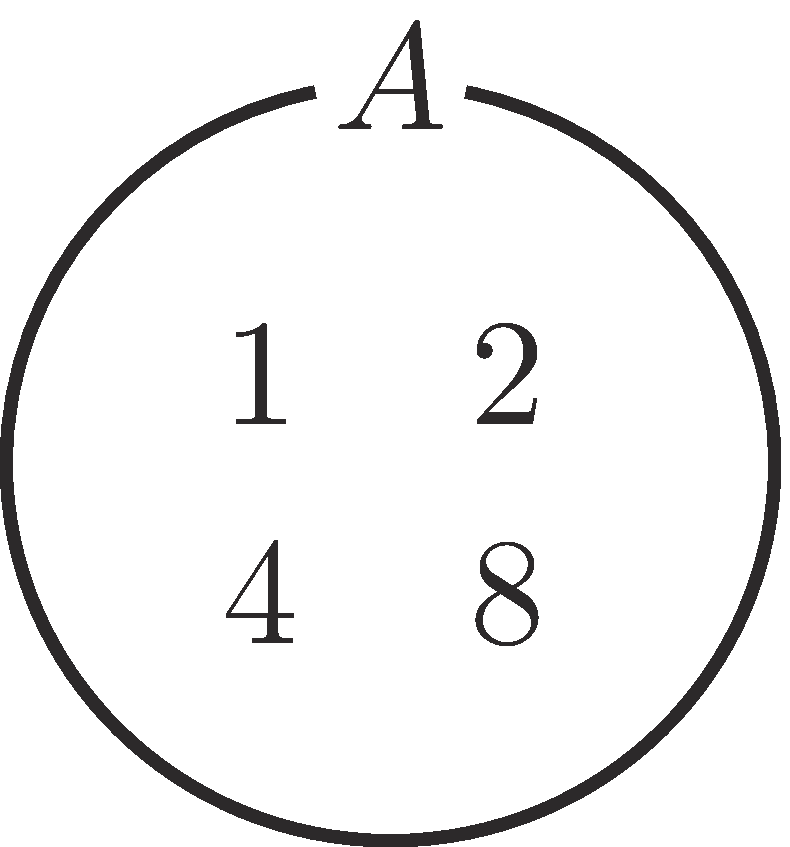
\includegraphics[scale=\pgfkeysvalueof{picsize}]{DBs/pic/zero_01.pdf}\
\end{center}세 번째 방법은 그림을 이용한 방법(\term{벤 다이어그램}{})입니다. 그림과 같이 집합을 원으로 표시하고, 원소를 원 안에 나열하는 것입니다.
\section{집합 사이의 포함 관계}

\subsection{부분집합과 진부분집합}
두 집합 $A$, $B$에 대하여 $A$의 모든 원소가 $B$에 속할 때, $A$를 $B$의 \term{부분집합}{}이라고 하며, $A \subset B$라 표기합니다. 한편 $A$의 원소 중에서 단 하나라도 $B$에 속하지 않는 원소가 있으면 $A$는 $B$의 부분집합이 아니며, 이를 $A \not\subset B$라 표기합니다.

집합 $A$의 모든 원소는 자기 자신인 $A$에 속하므로, 모든 집합은 자기 자신의 부분집합입니다. 또한 공집합은 모든 집합의 부분집합입니다.

어떤 집합에 대하여, 자기 자신이 아닌 부분집합을 그 집합의 \term{진부분집합}{}이라고 합니다. 즉 두 집합 $A$, $B$에 대하여 $A \subset B$이고 $A \neq B$일 때, $A$는 $B$의 진부분집합입니다.

\begin{remark}{부분집합의 개수와 진부분집합의 개수}
사실 이 내용은 확률과 통계의 `경우의 수'에서 다루지만, 어렵지 않은 내용이므로 가볍게 다루어봅시다.

$n\left( A \right) = k $인 집합의 원소를 각각 $a_1$, $a_2$, $\cdots$, $a_k$라 할 때, $A$의 부분집합 $B$에는 $a_1$이 속할 수도 있고, 속하지 않을 수도 있습니다. 이는 $a_2$, $a_3$, $\cdots$, $a_k$ 모두 마찬가지이고, 각각의 사건은 서로 동시에(잇달아) 일어납니다. 따라서 곱의 법칙에 의하여 $k$개의 $2$를 서로 곱하면 $2\times2\times\cdots\times2=2^k$이므로 서로 다른 $B$의 개수는 $2^k$입니다. 진부분집합의 개수는 이 값에서 `집합 자기 자신의 개수'인 $1$을 뺀 $2^k -1$입니다.
\end{remark}
\vskip-20pt
\subsection{두 집합 사이의 포함 관계}
\vskip-10pt
\begin{figure}[h]\centering \subfloat[][]{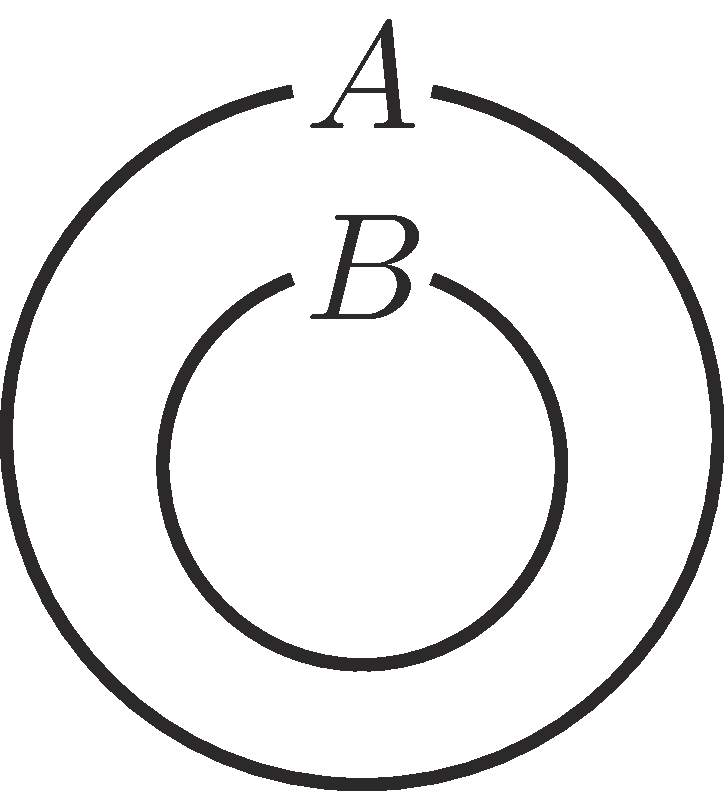
\includegraphics[scale=\pgfkeysvalueof{picsize}]{DBs/pic/zero_02_1.pdf}}\
\qquad
\centering \subfloat[][]{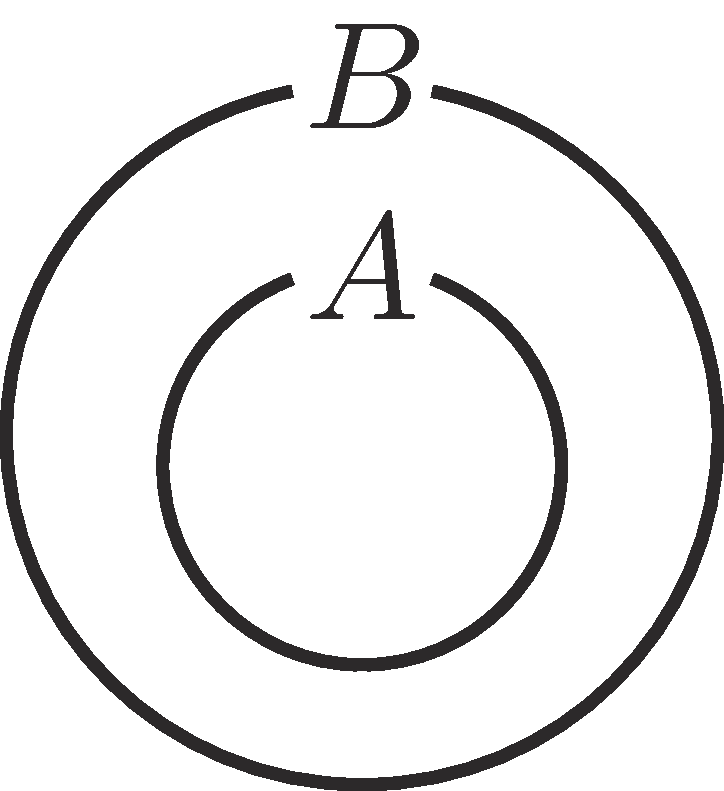
\includegraphics[scale=\pgfkeysvalueof{picsize}]{DBs/pic/zero_02_2.pdf}}\
\qquad
\centering \subfloat[][]{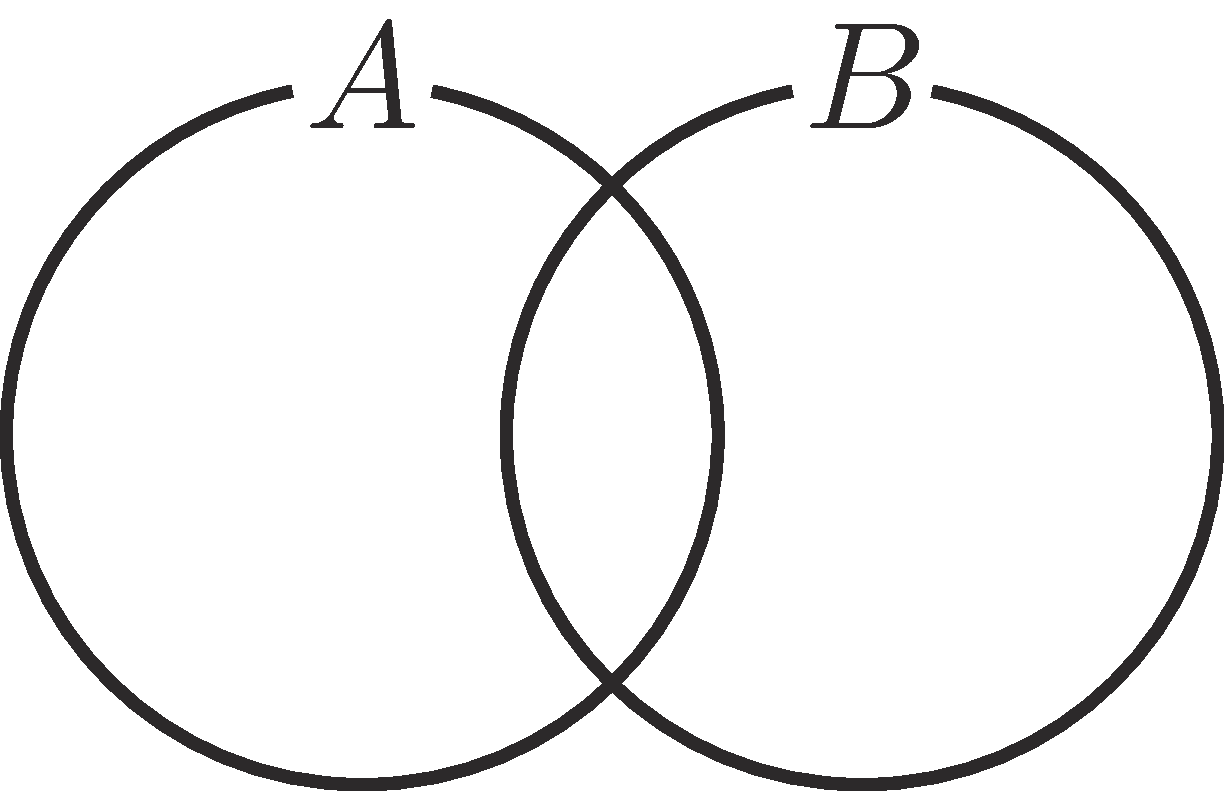
\includegraphics[scale=\pgfkeysvalueof{picsize}]{DBs/pic/zero_02_3.pdf}}\\
\centering \subfloat[][]{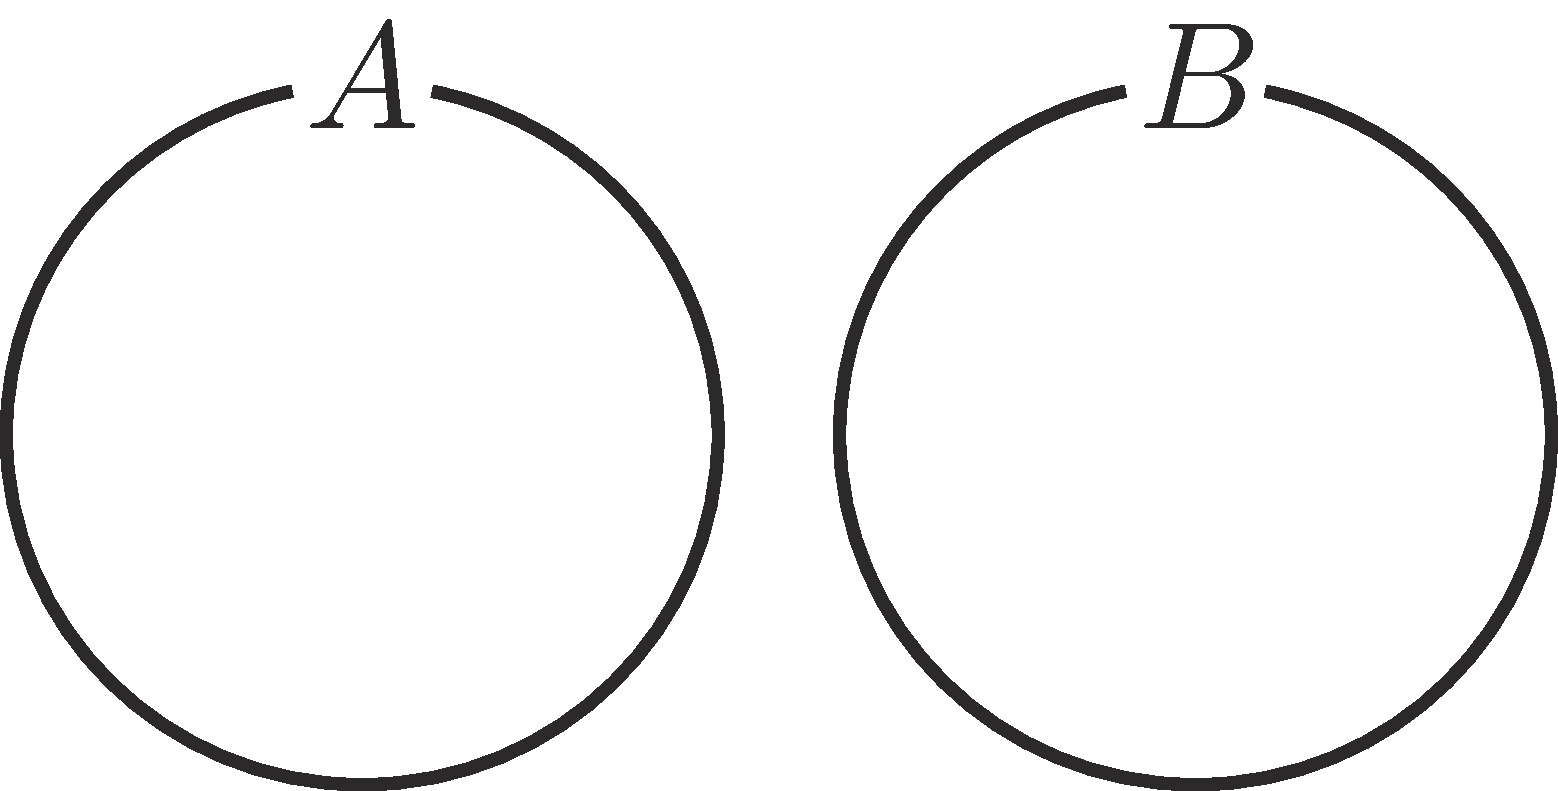
\includegraphics[scale=\pgfkeysvalueof{picsize}]{DBs/pic/zero_02_4.pdf}}\
\qquad
\centering \subfloat[][]{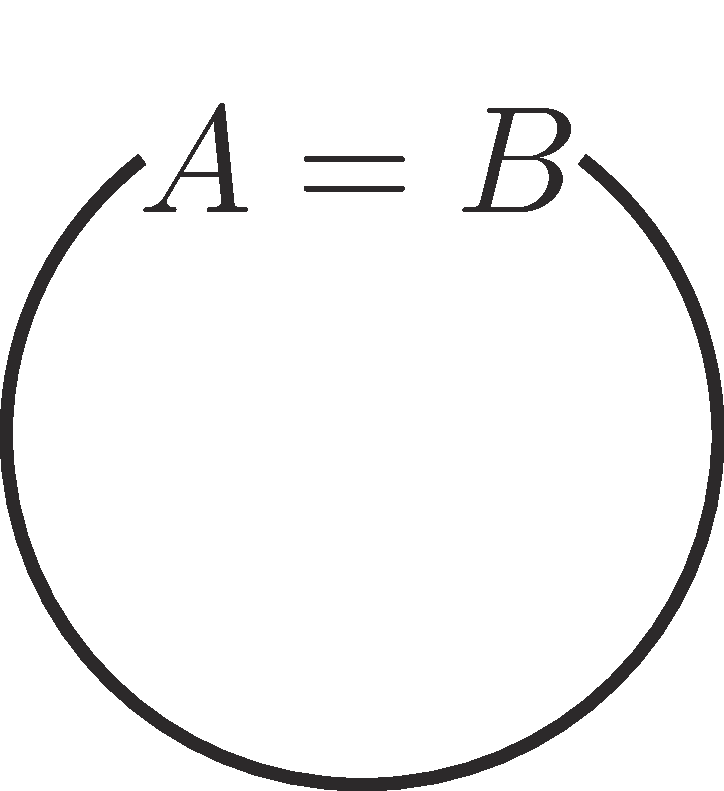
\includegraphics[scale=\pgfkeysvalueof{picsize}]{DBs/pic/zero_02_5.pdf}}\
\end{figure}\vskip-10pt


두 집합 $A$, $B$ 사이의 포함 관계는 그림과 같이 다섯 가지가 있습니다. (a), (b)는 한 집합이 다른 집합의 진부분집합인 경우입니다. (c)는 각 집합이 일부 원소만을 공유하는 경우입니다. (d)는 각 집합이 공유하는 원소가 없는 경우입니다. (e)는 두 집합이 서로 같은 경우입니다.

\section{집합의 연산}
\subsection{교집합, 합집합, 서로소}
\begin{center} 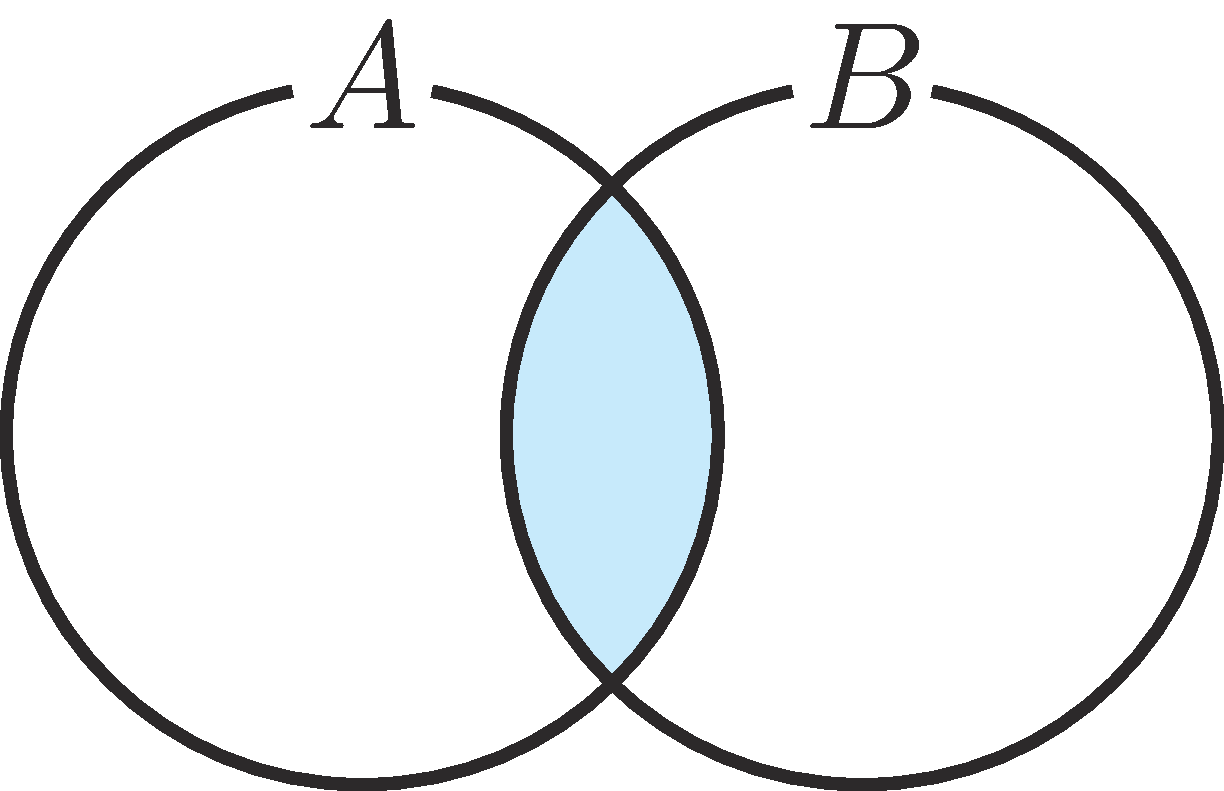
\includegraphics[scale=\pgfkeysvalueof{picsize}]{DBs/pic/zero_03.pdf}\
	\end{center}두 집합 $A$, $B$의 포함관계가 그림과 같을 때, 색칠된 부분은 $A$에도 속하고 $B$에도 속하는 원소들을 나타냅니다. 이러한 모든 원소로 이루어진 집합을 `$A$와 $B$의 \term{교집합}{}'이라 하며, $A \cap B$라 표기합니다. 이를 조건제시법으로 나타내면 다음과 같습니다.\mn{`속하고'라는 표현이 `그리고'로 바뀌는 것에 주목할 필요가 있습니다.}{} \begin{align*}A\cap B = \conset{x}{$x\in A$ 그리고 $x\in B$} \end{align*}
\begin{center} 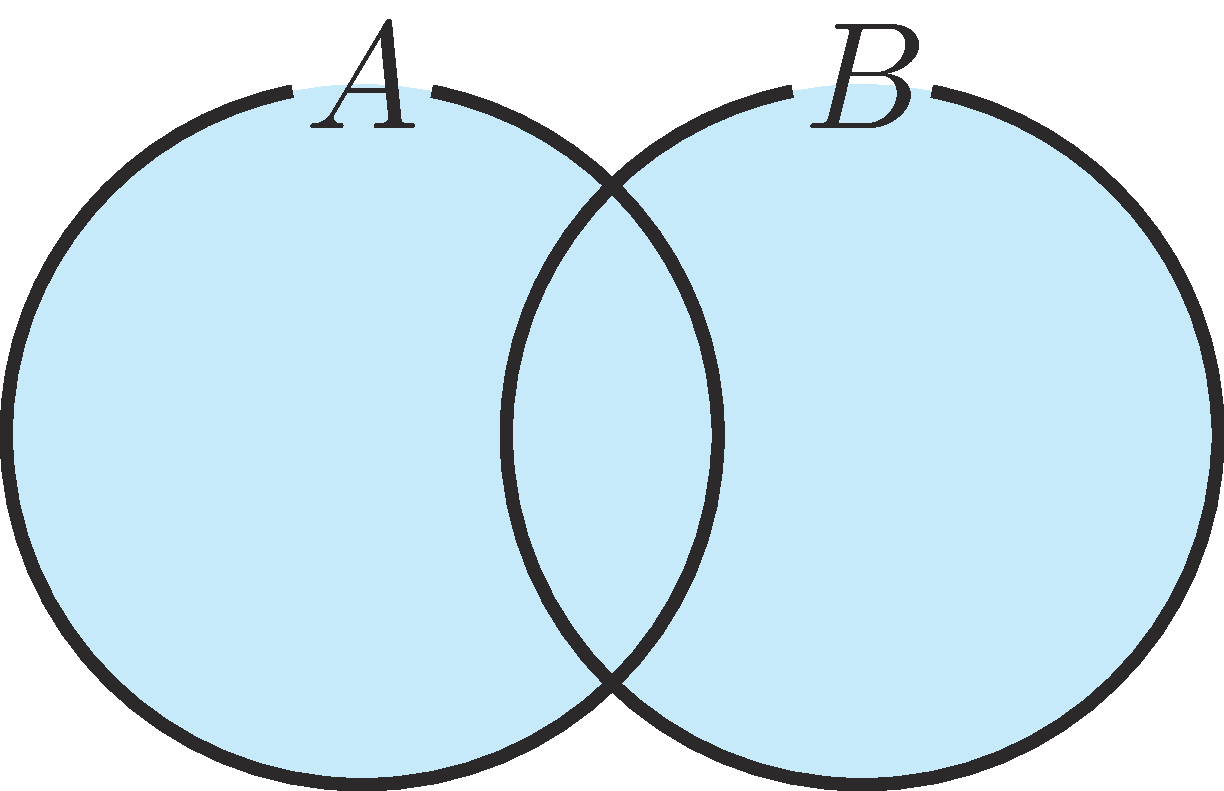
\includegraphics[scale=\pgfkeysvalueof{picsize}]{DBs/pic/zero_04.pdf}\
	\end{center}두 집합 $A$, $B$의 포함관계가 그림과 같을 때, 색칠된 부분은 $A$에 속하거나 $B$에 속하는 원소들을 나타냅니다. 이러한 모든 원소로 이루어진 집합을 `$A$와 $B$의 \term{합집합}{}'이라 하며, $A \cup B$라 표기합니다. 이를 조건제시법으로 나타내면 다음과 같습니다.\mn{`속하거나'라는 표현이 `또는'으로 바뀌는 것에 주목할 필요가 있습니다.}{} \begin{align*}A\cup B = \conset{x}{$x\in A$ 또는 $x\in B$} \end{align*}
\begin{center} 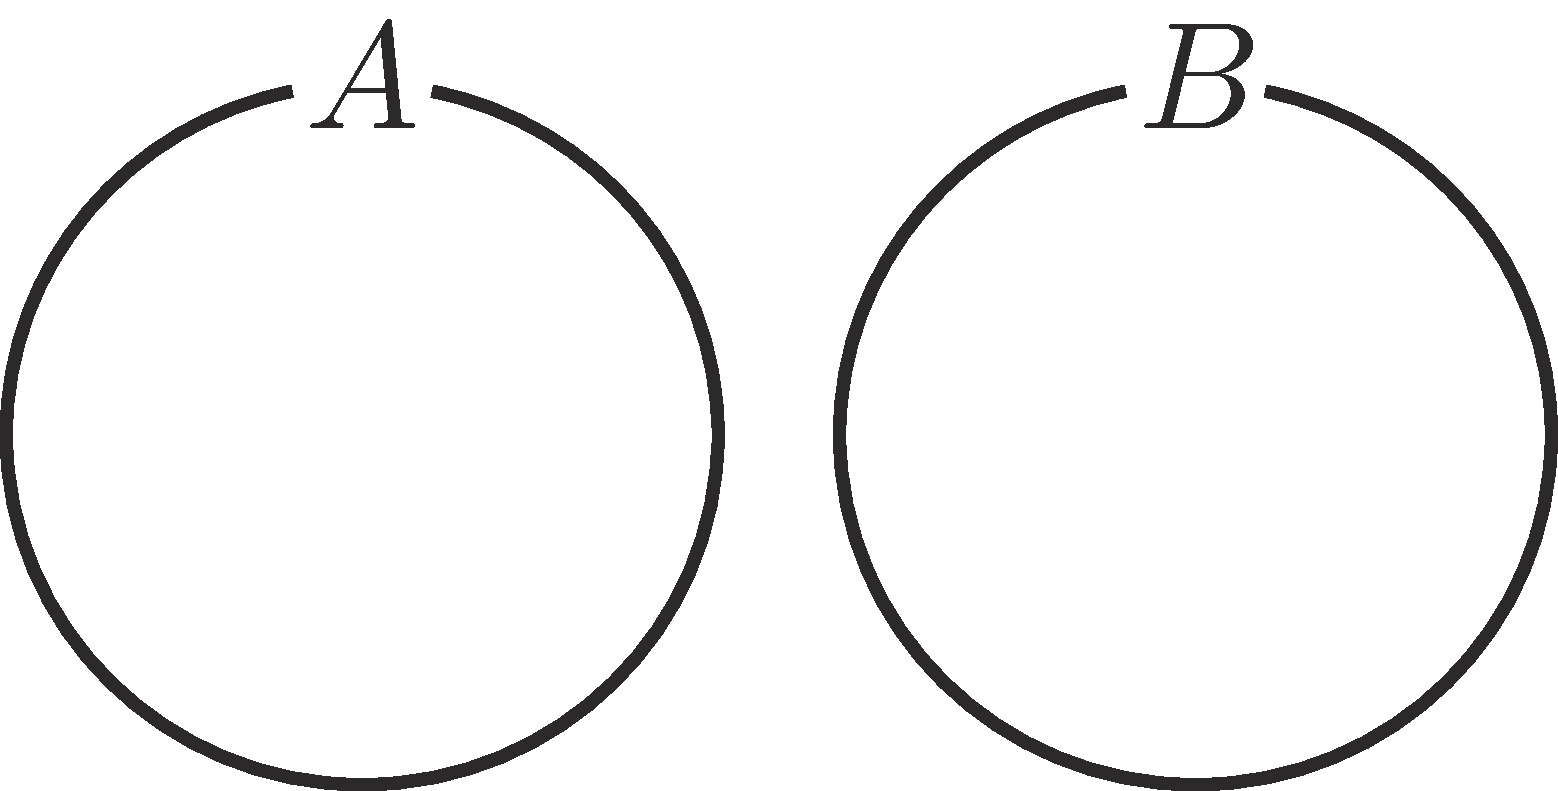
\includegraphics[scale=\pgfkeysvalueof{picsize}]{DBs/pic/zero_05.pdf}\
	\end{center}두 집합 $A$, $B$의 포함관계가 그림과 같아서 각 집합이 공유하는 원소가 없을 때, 즉 $A \cap B = \emptyset$인 경우, 두 집합 `$A$와 $B$는 \term{서로소}{}'라고 합니다.

\subsection{합집합의 원소의 개수}
원소의 개수가 유한개인 두 집합 $A$, $B$에 대하여 다음이 성립합니다.
\begin{align*}n\left( A\cup B \right) = n\left( A \right)  + n\left( B \right) - n\left( A \cap B \right)\end{align*}
\clearpage
\subsection{차집합}
\begin{center} 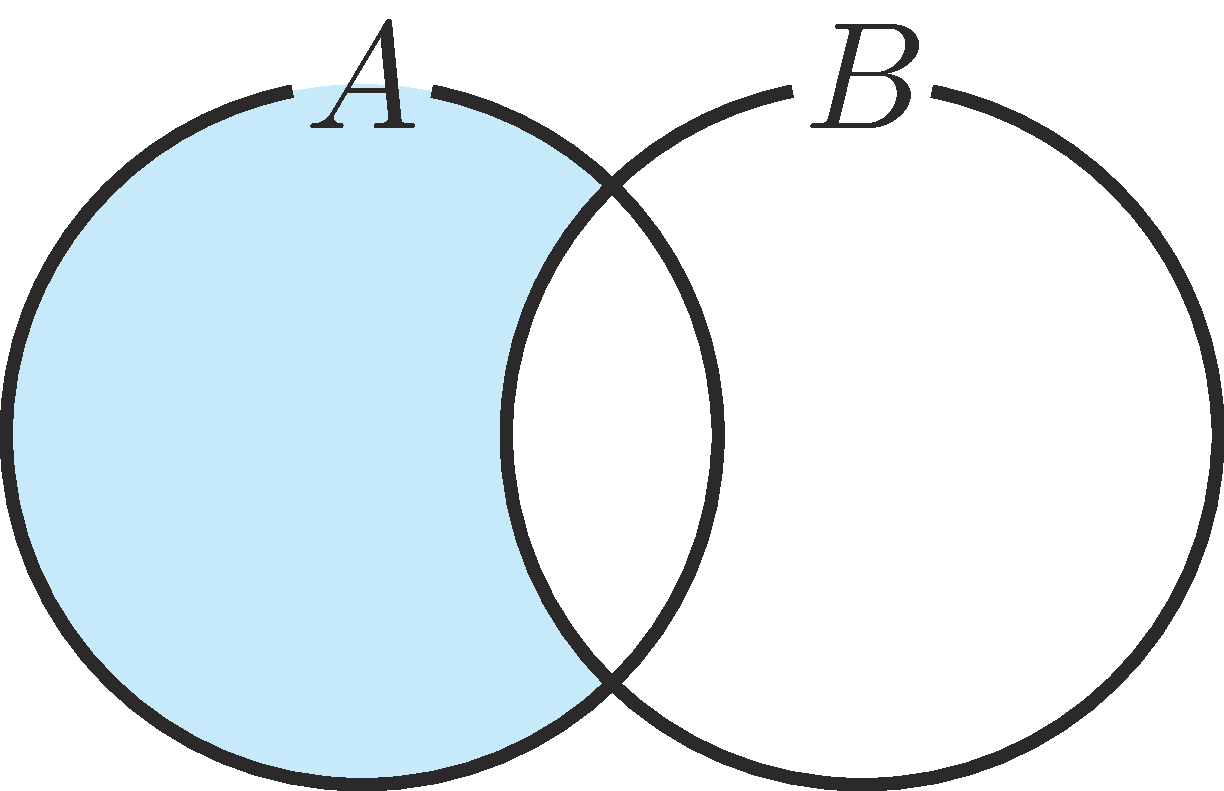
\includegraphics[scale=\pgfkeysvalueof{picsize}]{DBs/pic/zero_06.pdf}\
	\end{center}두 집합 $A$, $B$의 포함관계가 그림과 같을 때, 색칠된 부분은 $A$에는 속하고 $B$에는 속하지 않는 원소들을 나타냅니다. 이러한 모든 원소로 이루어진 집합을 `$A$에 대한 $B$의 \term{차집합}{}'이라 하며, $A - B$라 표기합니다. 이를 조건제시법으로 나타내면 다음과 같습니다.\mn{`속하고'라는 표현이 `그리고'로 바뀌는 것에 주목할 필요가 있습니다.}{} \begin{align*}A - B = \conset{x}{$x\in A$ 그리고 $x\not\in B$} \end{align*}

\subsection{전체집합과 여집합}
\begin{center} 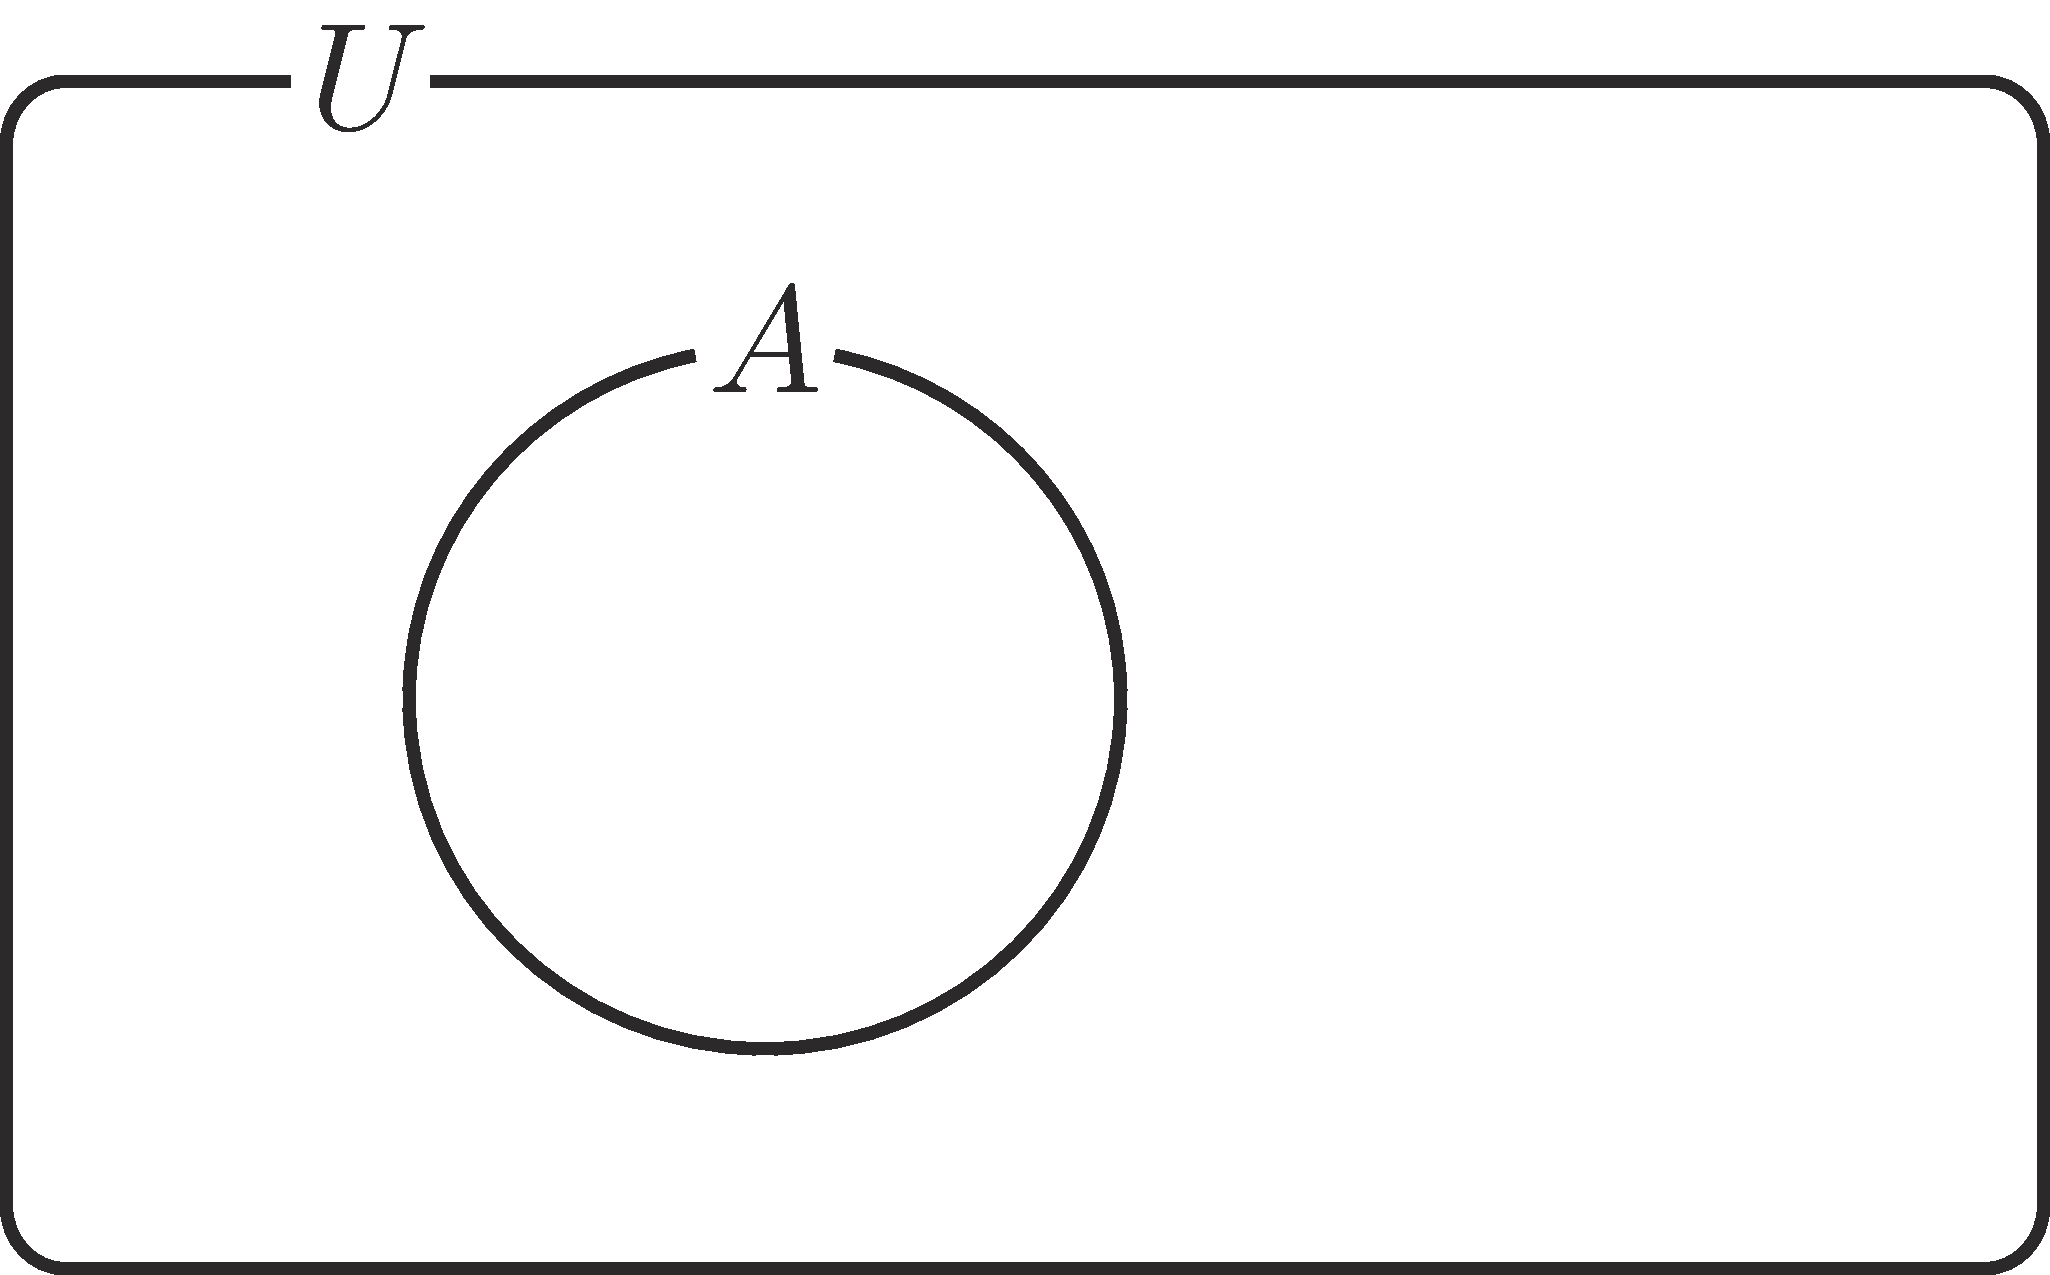
\includegraphics[scale=\pgfkeysvalueof{picsize}]{DBs/pic/zero_07.pdf}\
	\end{center}주어진 어떤 집합에 대하여 그의 부분집합을 생각할 때, 처음에 주어진 집합을 \term{전체집합}{}이라고 하며, $U$라 표기합니다. 전체집합을 벤 다이어그램에 나타낼 때, 관습적으로 모서리가 둥근 네모꼴로 나타냅니다.
\begin{center} 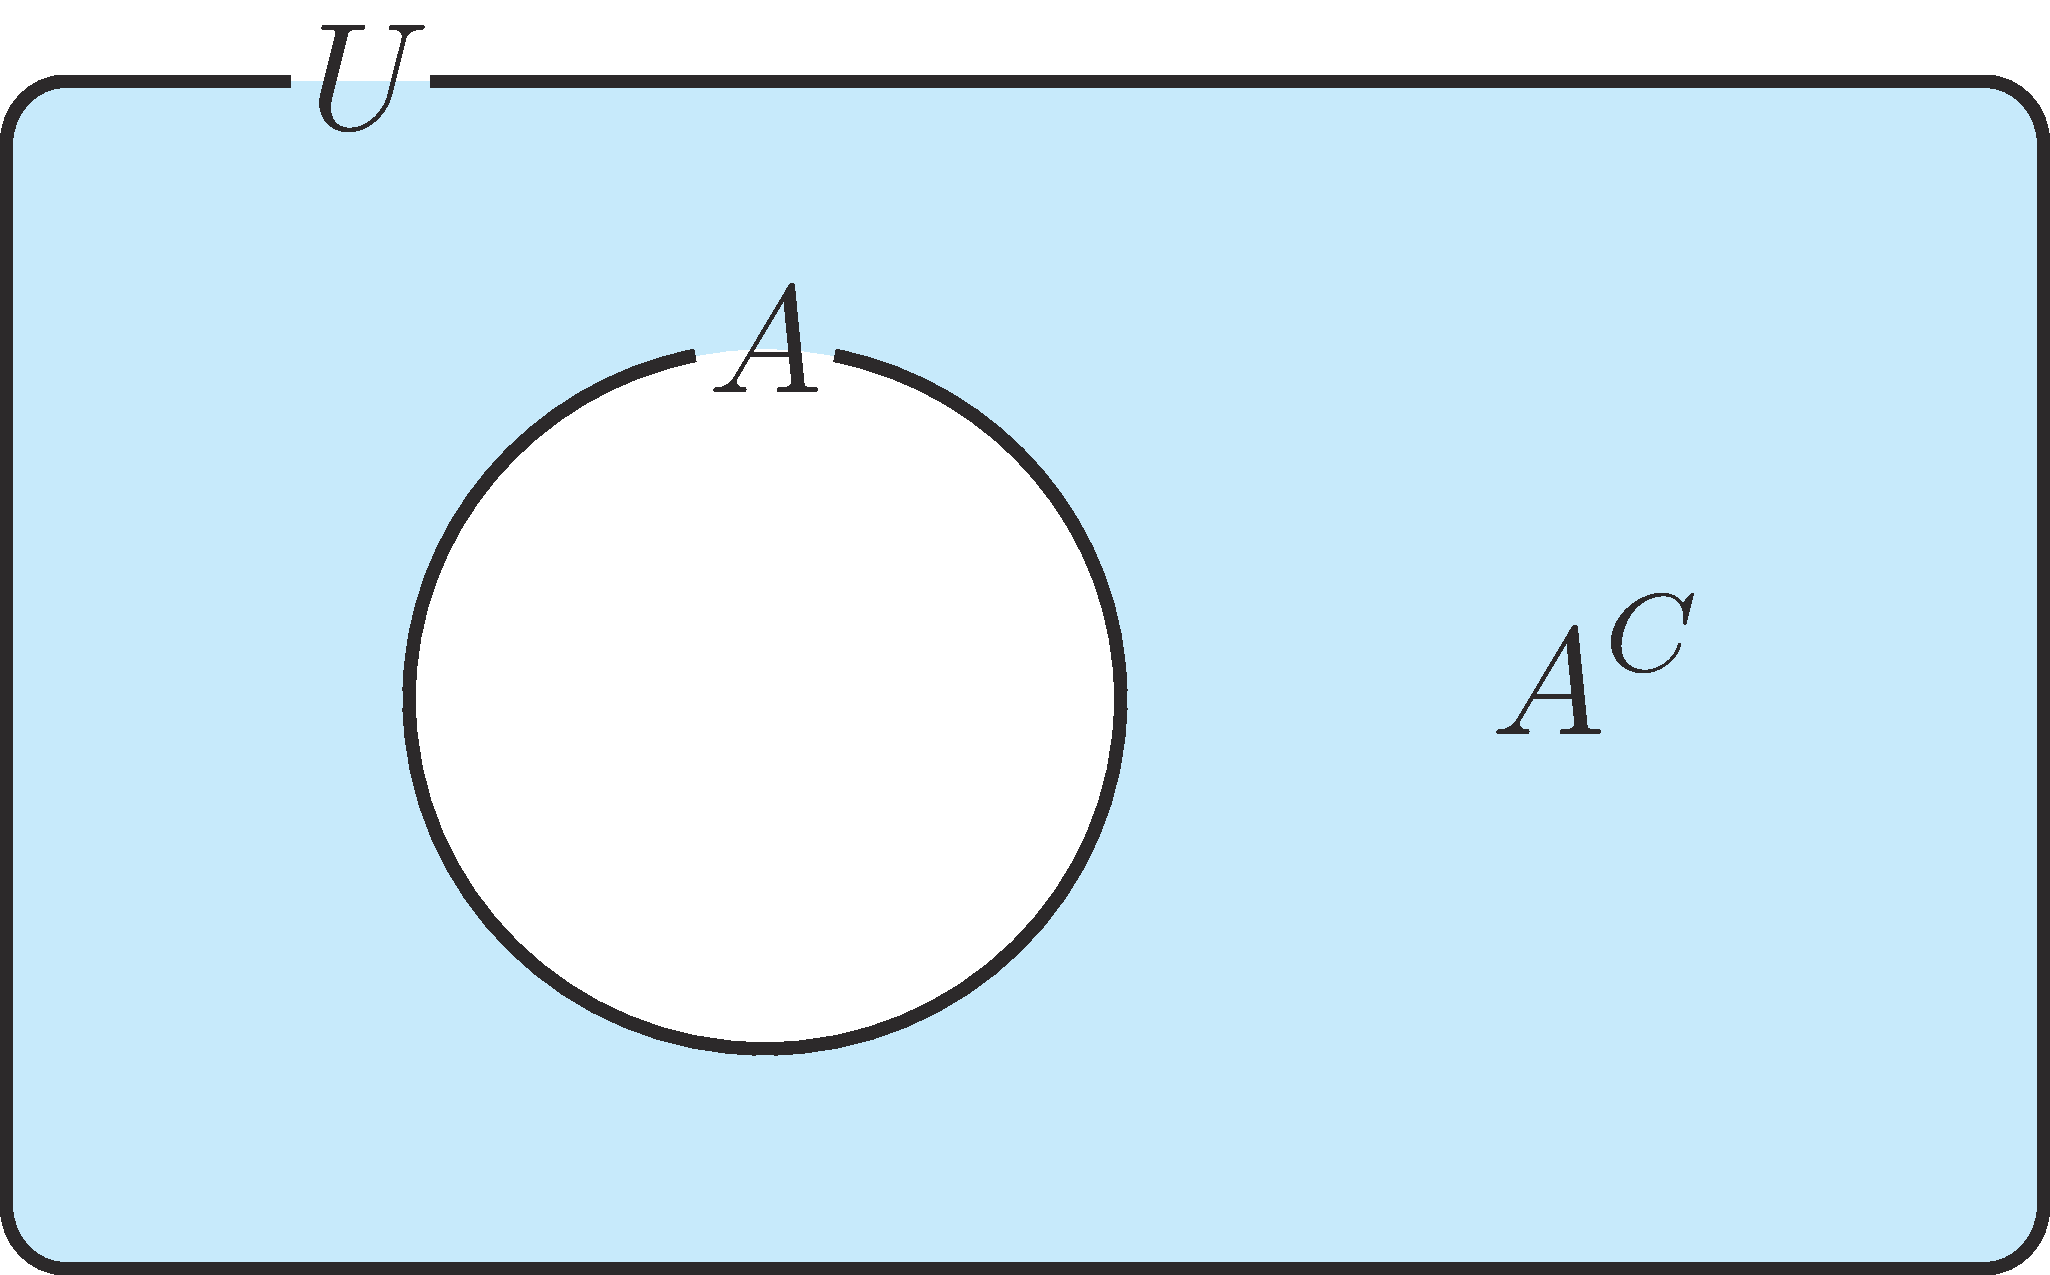
\includegraphics[scale=\pgfkeysvalueof{picsize}]{DBs/pic/zero_08.pdf}\
	\end{center}전체집합 $U$의 부분집합 $A$에 대하여 $U$의 원소 중에서 $A$에 속하지 않는 모든 원소로 이루어진 집합을 `$U$에 대한 $A$의 \term{여집합}{}'이라고 하며, $A^C$라 표기합니다. 이를 조건제시법으로 나타내면 다음과 같습니다.\begin{align*}A^C= \conset{x}{$x\in U$ 그리고 $x\not\in A$} \end{align*}

\clearpage
\section{집합의 연산}
\subsection{전체집합, 여집합, 차집합의 연산}
\begin{center} 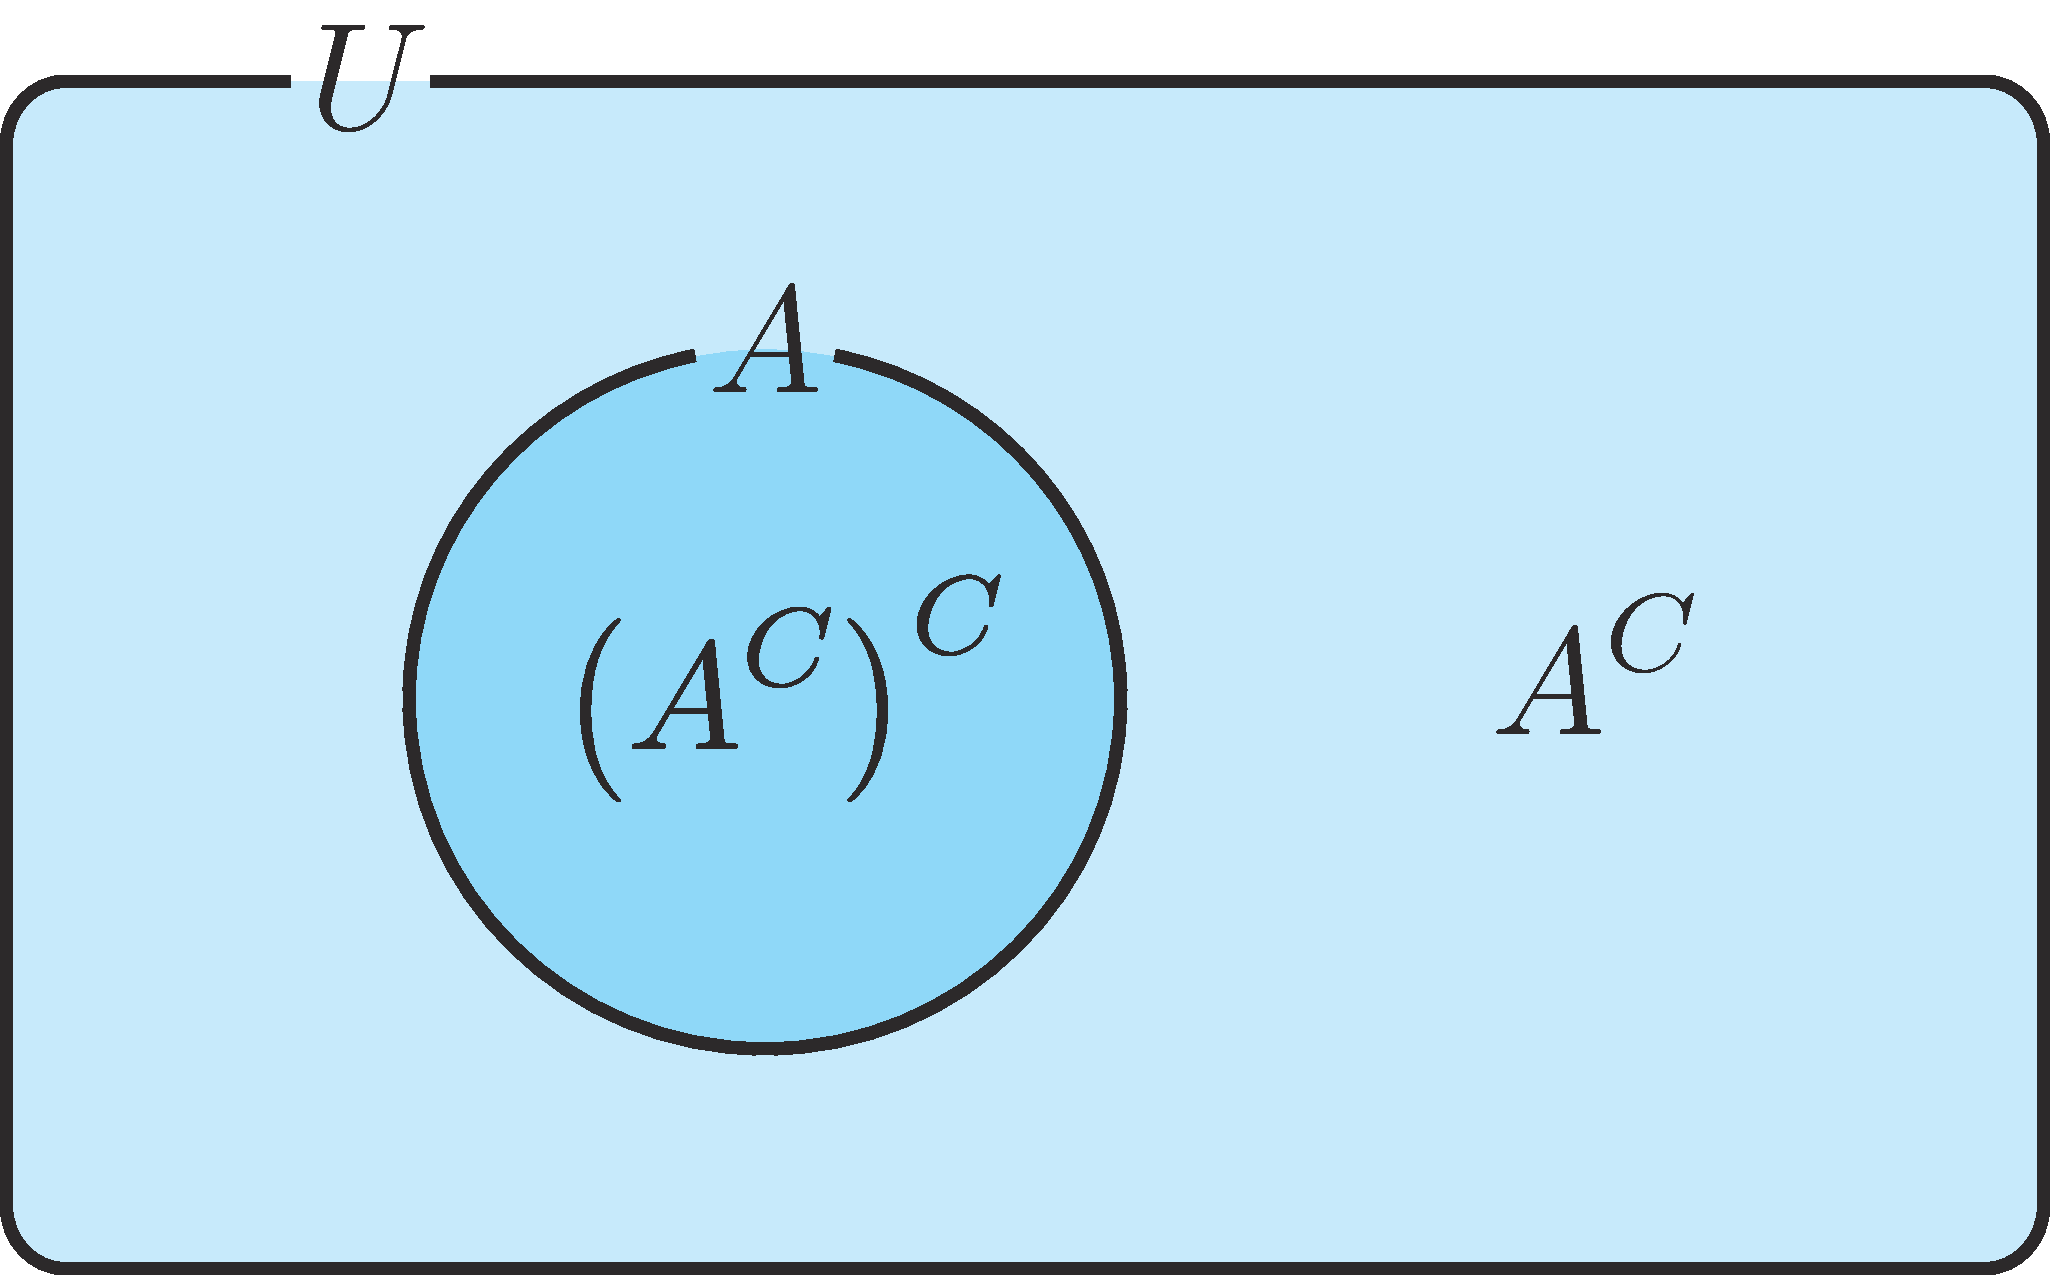
\includegraphics[scale=\pgfkeysvalueof{picsize}]{DBs/pic/zero_09.pdf}\
	\end{center}전체집합 $U$의 부분집합 $A$에 대하여, $A\cup A^C = U$, $\left( A^C \right)^C = A $가 성립합니다. 위 그림은 이 연산을 벤 다이어그램으로 나타낸 것입니다.
\begin{center} 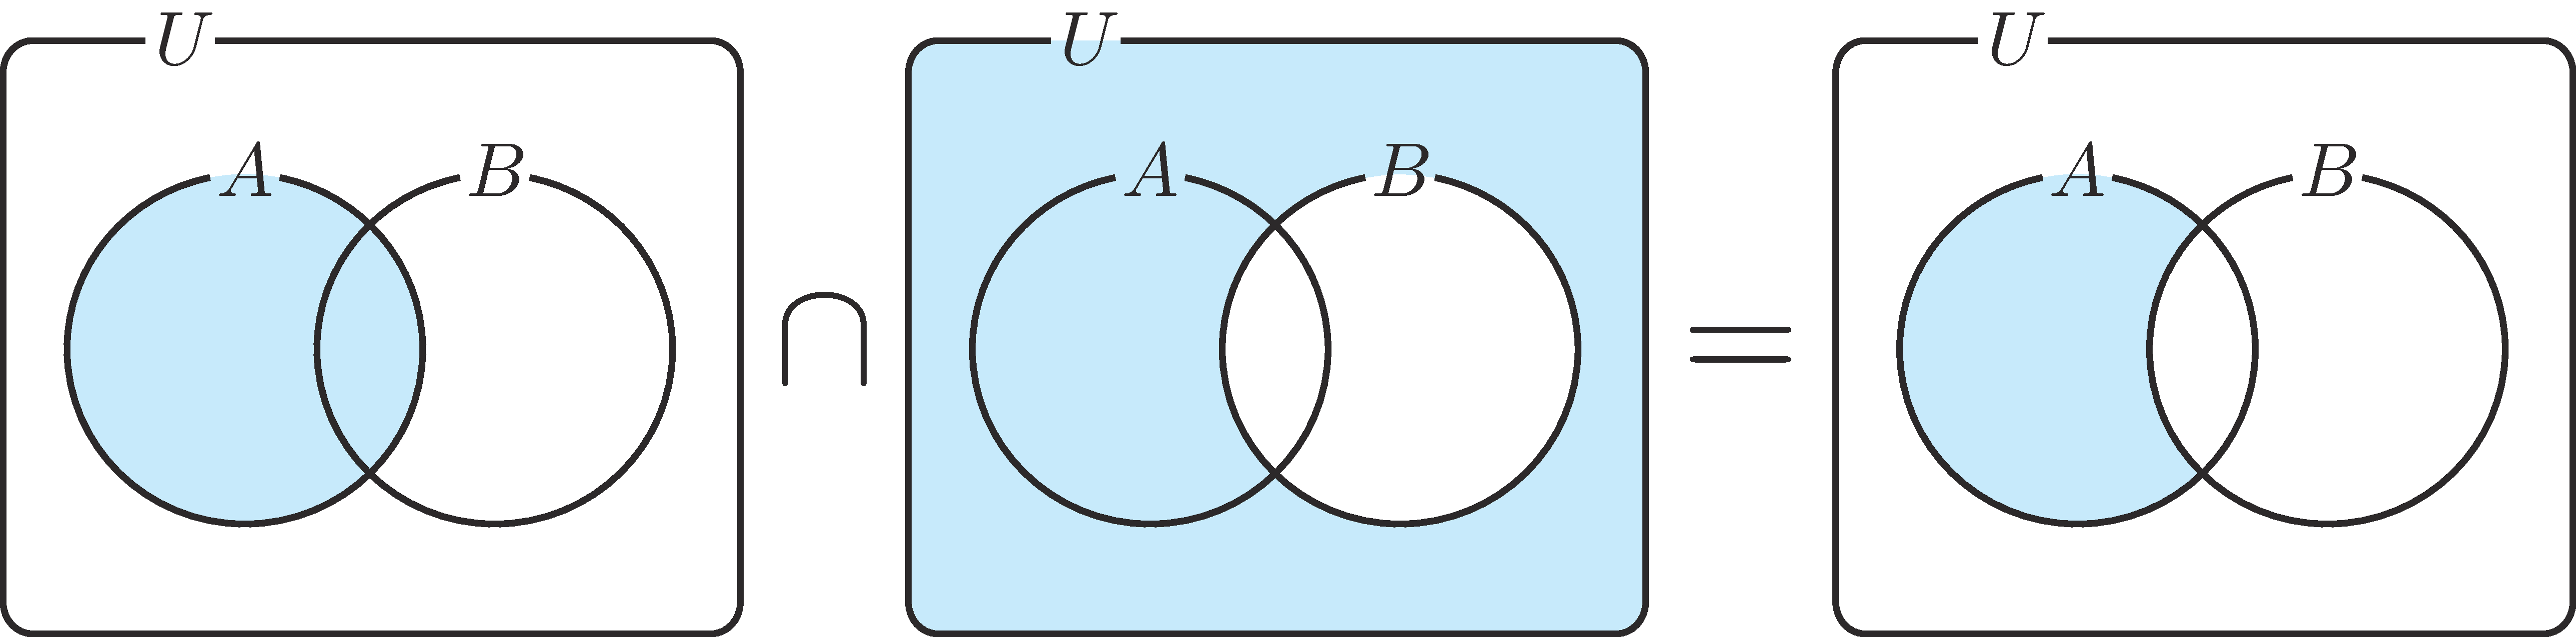
\includegraphics[scale=\pgfkeysvalueof{picsize}]{DBs/pic/zero_10.pdf}\
	\end{center}전체집합 $U$에 속하는 두 집합 $A$, $B$의 포함관계가 그림과 같은 경우, 여집합 기호와 집합의 연산을 이용하여 $A$에 대한 $B$의 차집합을 $A\cap B^C$와 같이 표현할 수 있습니다. 위 그림은 이 연산을 벤 다이어그램으로 나타낸 것입니다.
\begin{center} 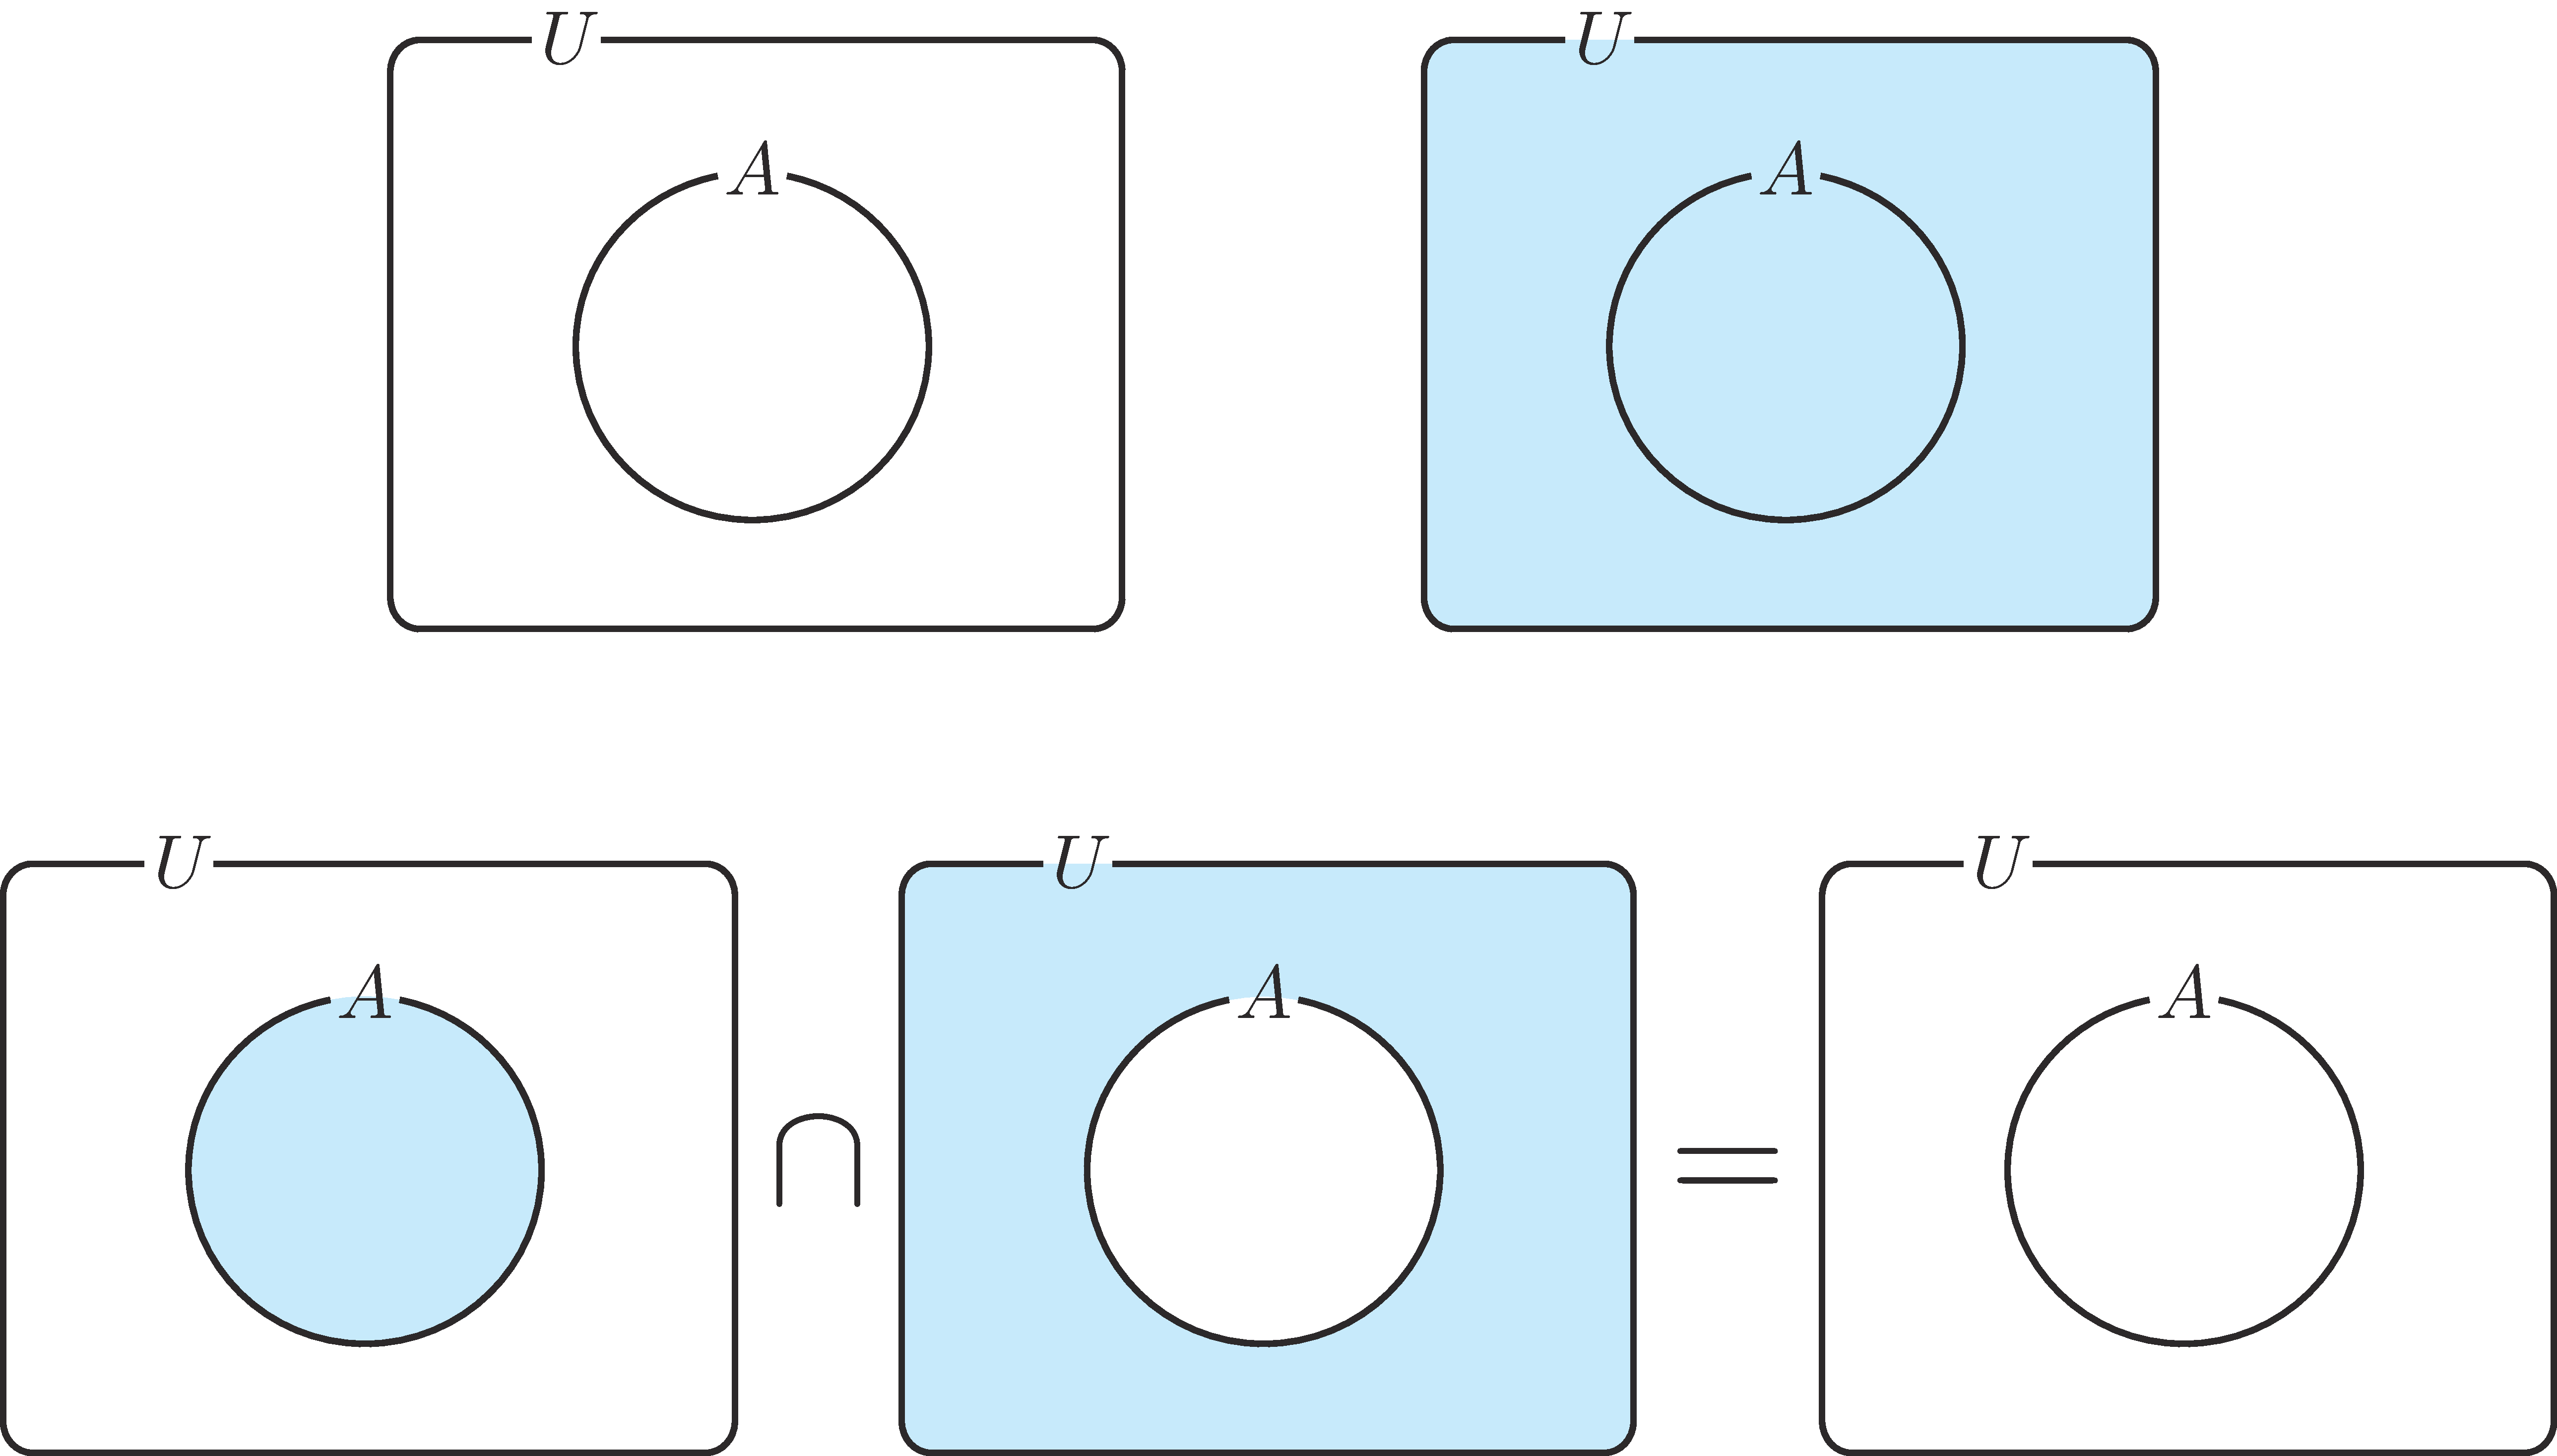
\includegraphics[scale=\pgfkeysvalueof{picsize}]{DBs/pic/zero_10_1.pdf}\
	\end{center}앞서 배운 연산을 이용하여 $U^C=\emptyset$, $\emptyset^C=U$,  $A \cap A^C = \emptyset$이 성립함을 보일 수 있습니다. 위 그림은 각각의 상황을 나타낸 것입니다.

\clearpage
\subsection{교환법칙}
일반적으로 두 집합 $A$, $B$에 대하여 다음이 성립하며, 이를 각각 합집합에 대한 \term{교환법칙}{}, 교집합에 대한 \term{교환법칙}{}이라고 합니다.
\begin{align*}
    A\cup B =& B \cup A\\
    A\cap B =& B \cap A
\end{align*}
\subsection{결합법칙}
일반적으로 세 집합 $A$, $B$, $C$에 대하여 다음이 성립하며, 이를 각각 합집합에 대한 \term{결합법칙}{}, 교집합에 대한 \term{결합법칙}{}이라고 합니다.
\begin{align*}
    \left( A\cup B \right) \cup C &= A\cup \left( B\cup C  \right) = A\cup B \cup C \\
    \left( A\cap B \right) \cap C &= A\cap \left( B\cap C  \right) =  A\cap B \cap C
\end{align*}

\subsection{분배법칙}
일반적으로 세 집합 $A$, $B$, $C$에 대하여 다음이 성립하며, 이를 집합의 연산에 대한 \term{분배법칙}{}이라고 합니다.
\begin{align*}
    A \cap\left( B \cup C  \right) &= \left( A \cap B \right) \cup \left( A\cap C \right)   \\
    A \cup\left( B \cap C  \right) &= \left( A \cup B \right) \cap \left( A\cup C \right) 
\end{align*}

\subsection{드모르간의 법칙}
일반적으로 전체집합 $U$의 두 부분집합 $A$, $B$에 대하여 다음과 같은 연산법칙이 성립합니다. 이를 \term{드모르간의 법칙}{}이라고 합니다.\mn{윗첨자 자리의 ${}^C$를 $A$, $B$에 각각 분배하고, 연산기호는 뒤집어준다고 생각하면 외우기 쉽습니다.}{}
\begin{align*}
\left( A \cup B \right)^C &=A^C \cap B^C \\
\left( A \cap B \right)^C &=A^C \cup B^C \\
\end{align*}


\mychapter{실수 체계와 구간표기법}{}

\section{실수 체계}
\subsection{자연수 집합 $\mathbb{N}$과 정수 집합 $\mathbb{Z}$}
\term{자연수}{}는 $1$, $2$, $3$, $4$, $\cdots$와 같은 수를 말합니다. \term{정수}{}는 $\cdots$, $-3$, $-2$, $-1$, $0$, $1$, $2$, $3$, $\cdots$과 같은 수를 말합니다.  자연수 전체를 원소로 갖는 집합을 $\mathbb{N}$, 정수 전체를 원소로 갖는 집합을 $\mathbb{Z}$라 부르기로 합시다.

\subsection{유리수 집합 $\mathbb{Q}$}
$n \in \mathbb{Z}$, $m \in \mathbb{Z}$이고 $n \ne 0$일 때, \term{유리수}{}는 $\dfrac{m}{n}$의 꼴, 즉 두 정수의 분수꼴로 나타낼 수 있는 수를 말합니다. 유리수 전체를 원소로 갖는 집합을 $\mathbb{Q}$라 부르기로 합시다. 이를 조건제시법으로 나타내면 다음과 같습니다.
\begin{align*}\mathbb{Q} = \conset[\bigg]{\dfrac{m}{n}}{$n\in\left(  \mathbb{Z}-\left\{ 0 \right\} \right)   $이고 $m\in \mathbb{Z}$}\end{align*}

유리수는 정수와 \term{정수가 아닌 유리수}{}로 나뉩니다. 정수가 아닌 유리수는 \term{기약분수}{}\mn{분수 $\dfrac{q}{p}$에서 $p$와 $q$의 최대공약수가 $1$인 경우,\mnpar 즉 $p$와 $q$가 서로소인 경우입니다.}{}로 나타내는 경우가 많습니다.
\begin{center} 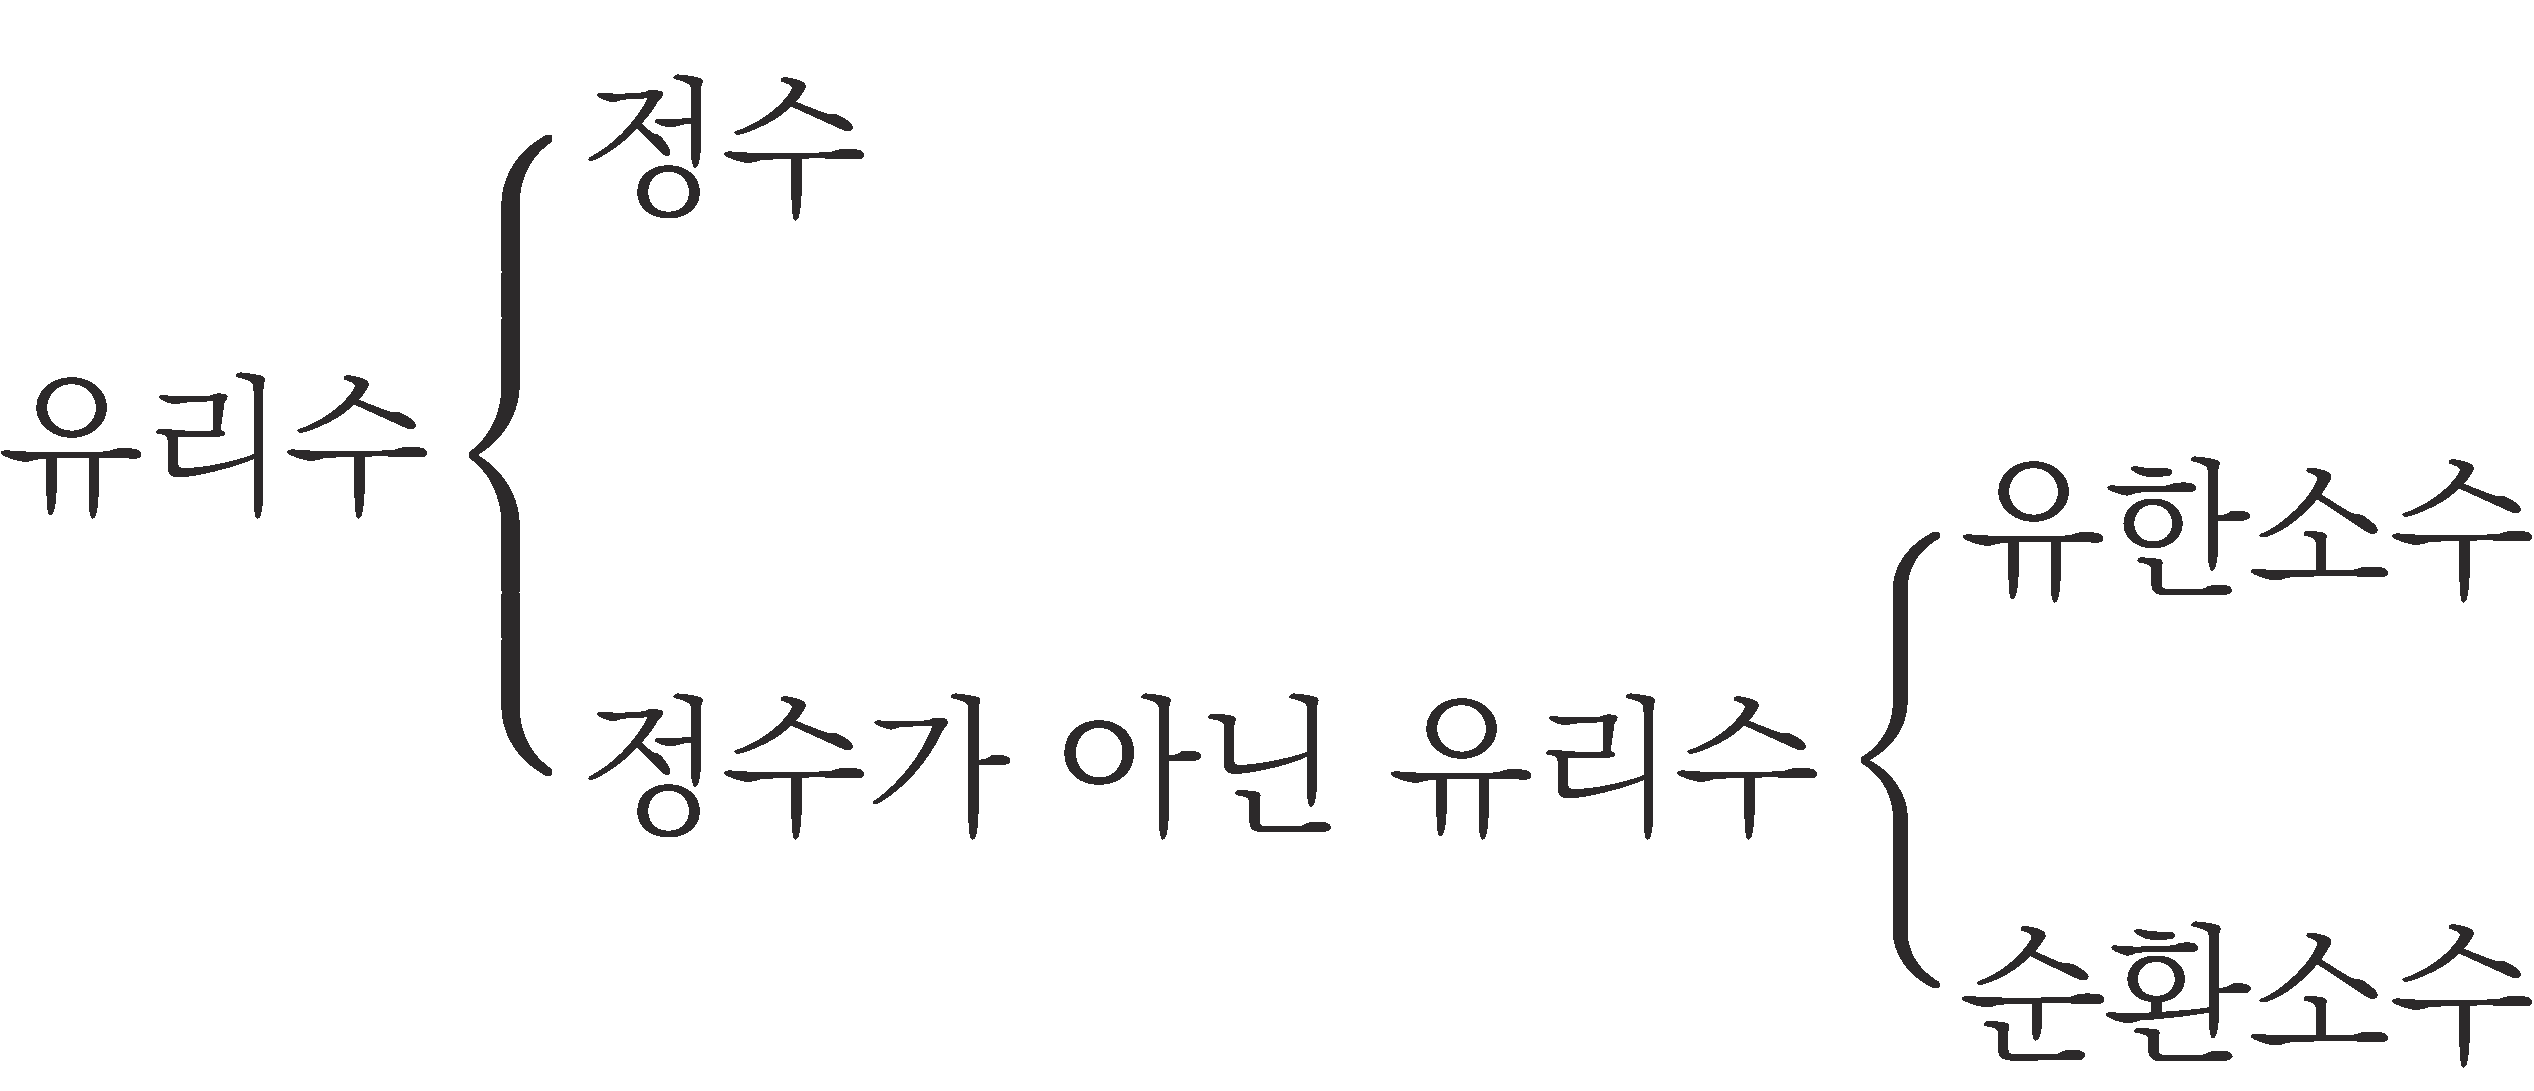
\includegraphics[scale=\pgfkeysvalueof{picsize}]{DBs/pic/zero_11.pdf}\
	\end{center}정수가 아닌 유리수는 \term{유한소수}{}와 \term{순환소수}{}로 나뉩니다. 유한소수는 $\dfrac{548}{1000}=0.548$과 같이 소수점 이후의 자리가 유한한 소수이고, 순환소수는 $\dfrac{1}{3}=0.33333\cdots=0.\dot3$, $\dfrac{919}{999}=0.919919919919\cdots=0.\dot91\dot9$, $\dfrac{53}{90}=0.5888\cdots=0.5\dot8$과 같이 소수점 이후의 일부 또는 전부의 자릿값이 규칙적으로 순환하는 무한소수입니다.\mn{규칙적으로 순환하지 않는 무한소수는 비순환소수라 하며, 이는 무리수입니다.}{}

\subsection{무리수 집합 $\mathbb{I}$}
$\pi = 3.141592\cdots$, $e = 2.7182818\cdots$와 같이 규칙적으로 순환하지 않는 무한소수를 \term{비순환소수}{}라 합니다. 모든 비순환소수는 \term{무리수}{}이고, 모든 무리수는 비순환소수입니다. 무리수의 집합을 $\mathbb{I}$라 부르기로 합시다.\mn{대학에서는 새로운 차집합 기호인 $\setminus$를 이용해 $\mathbb R \setminus \mathbb Q$라 표현하는 방법이 더 널리 쓰입니다.}{}

\subsection{실수 집합 $\mathbb{R}$}
유리수와 무리수를 통틀어 \term{실수}{}라고 합니다. 실수 전체를 원소로 갖는 집합을 $\mathbb{R}$라 부르기로 합시다. 이를 조건제시법으로 나타내면 다음과 같습니다. \begin{align*}\mathbb{R} = \conset{x}{$x\in \mathbb{Q} $ 또는 $x\in \mathbb{I}$}\end{align*}
\cleartorecto
\subsubsection{수직선}\begin{center} 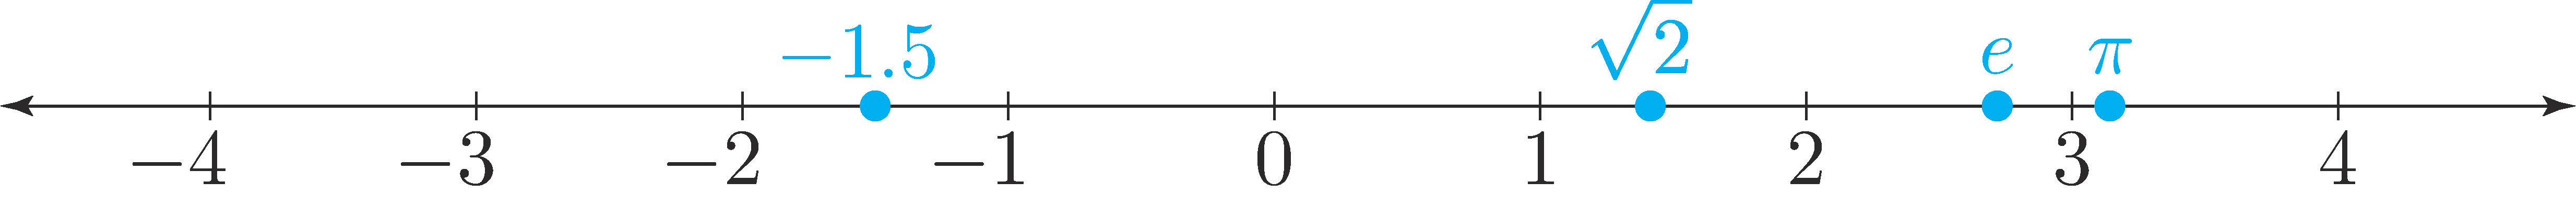
\includegraphics[scale=\pgfkeysvalueof{picsize}]{DBs/pic/zero_11_1.pdf}\
	\end{center}실수 집합은 직선, 실수 집합의 원소는 그 직선 위의 한 점에 대응됩니다. 이렇게 실수를 나타내는 직선을 \term{수직선}{}이라 합니다.
\section{실수를 바라보는 관점}

\subsection{정수의 여부 : 정수인가, 정수가 아닌가}
주어진 실수가 정수(자연수)일 때와 그렇지 않을 때는 다루는데 큰 차이가 두 가지 있습니다.

첫째, 정수(자연수)일 때에는 `주어진 수보다 큰 수 중에서 가장 작은 수'라는 개념과 `주어진 수보다 작은 수 중에서 가장 큰 수'라는 개념이 존재하지만, 실수에서는 존재하지 않습니다.

둘째, 범위가 한정되었을 때\mn{이를 테면 $-10<x<10$인 $x$} 정수(자연수)의 개수는 몇 개 되지 않으므로 따져야 할 경우가 한정되지만, 실수의 개수는 무수히 많으므로 경우별로 다룰 수는 없고 범위에 따라 다루어야 합니다.

\subsection{부호에 따라 : 양수인가, 음수인가, $0$인가}
수학에서는 주어진 실수의 부호가 무엇이냐가 중요한 경우가 굉장히 많습니다. 제곱할 때, 제곱근을 취할 때, 절댓값을 취할 때 부호에 주의해야 하는 것 또한 부호에 따라 그 값이 달라지기 때문입니다.
\clearpage

\section{구간표기법}
\subsection{구간표기법이 필요한 이유}
부등식의 해를 통해 어떤 실수인 변수가 취하는 범위를 나타낼 수 있습니다. 가령 $2$ 이상 $3$ 이하인 실수 $x$의 범위는 $2 \le x \le 3$입니다. 이 부등식의 해를 원소로 하는 집합 $X=\left\{x \mid 2 \le x \le 3\right\}$를 생각할 수도 있습니다.

그러나 매번 부등식이나 집합의 조건제시법으로 범위를 나타내기는 번거롭습니다. 부등식이나 집합 없이 간단하게 범위를 표현하기 위한 방법인 \iterm{구간표기법}{}을 배워봅시다. 

\subsection{범위의 양쪽 끝이 모두 제한되어 있을 때}
\begin{center} 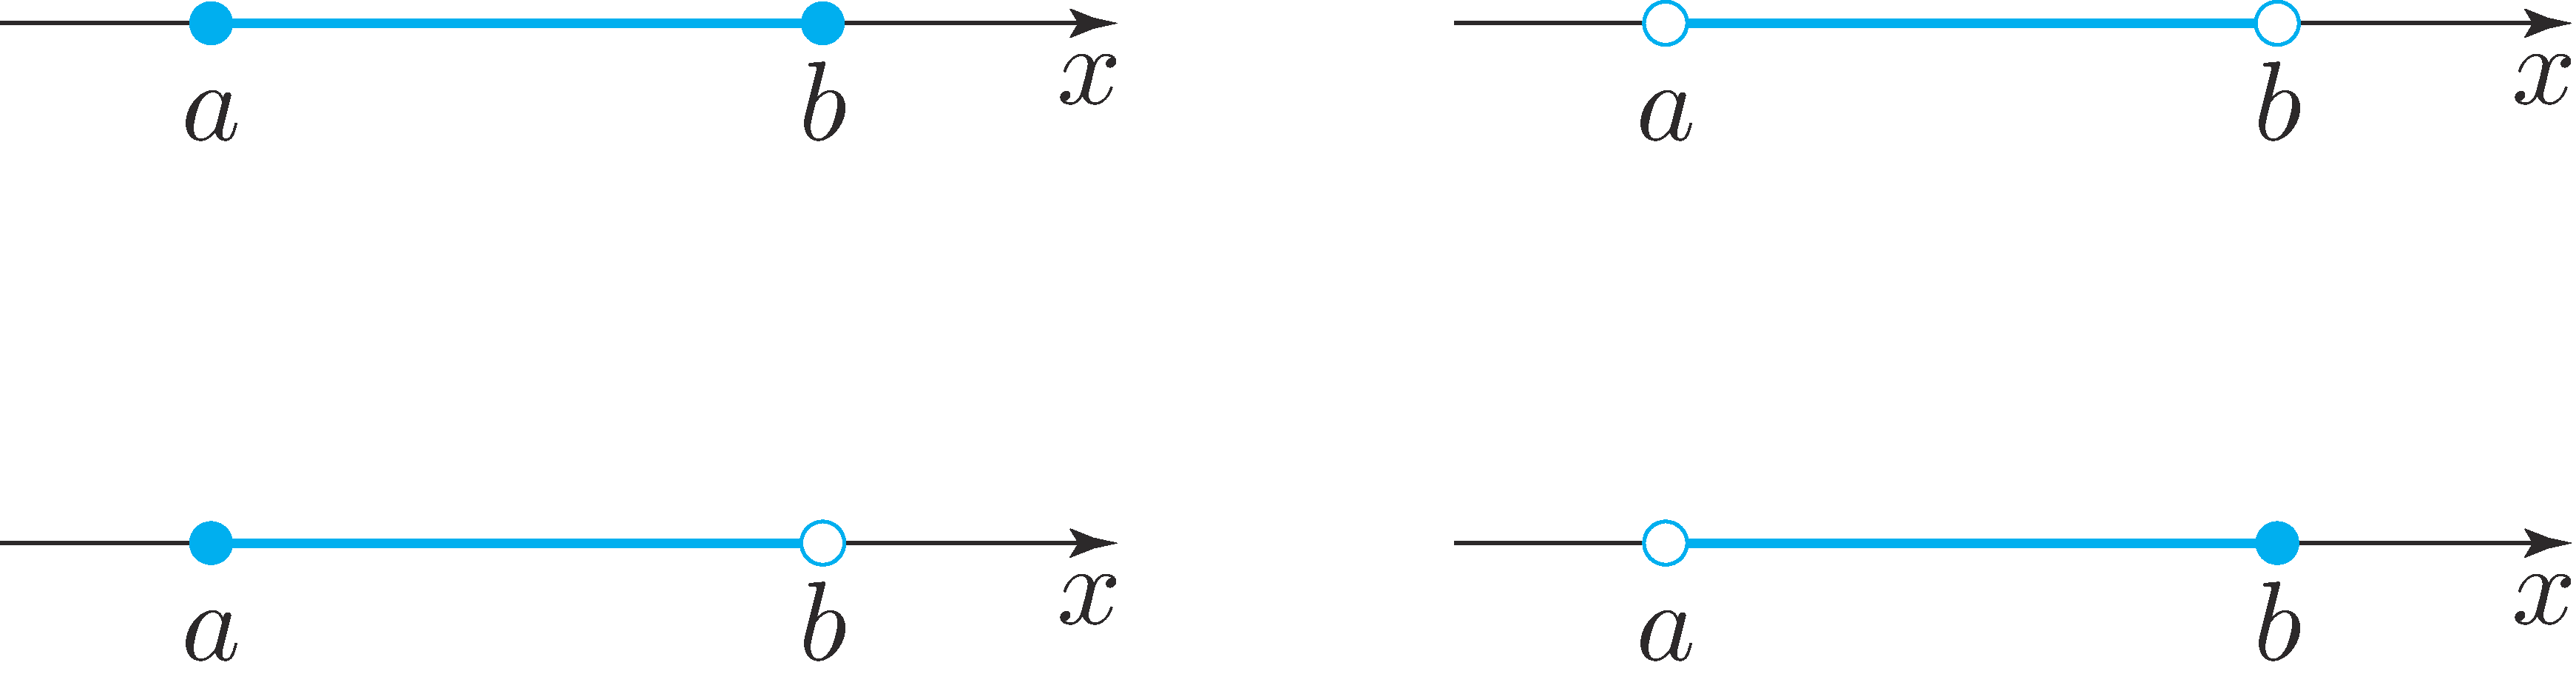
\includegraphics[scale=\pgfkeysvalueof{picsize}]{DBs/pic/zero_12.pdf}\
	\end{center}위 그림과 같이 범위의 양쪽 끝이 각각 서로 다른 실수 $a$, $b$ ($a<b$)로 제한되어 있을 때, $a$ 또는 $b$의 포함 여부에 따라 다음과 같이 $4$가지의 범위를 생각할 수 있습니다.
\begin{align*}
a \le x \le b, \: &&a < x < b, \\
a \le x < b, \: &&a < x \le b
\end{align*}
부등식 $a \le x \le b$를 만족하는 실수 $x$의 범위를 $\CCI{a}{b}$라 표기하고, 이를 `\term{닫힌구간}{} 에이 비'라 읽습니다. $a$를 \iterm{구간의 왼쪽 끝}{}, $b$를 \iterm{구간의 오른쪽 끝}이라고 부르기로 합시다.%\mn[-4em]{각각 하한(infimum, the greatest lower bound), 상한(supremum, the least upper bound)라는 해석학 용어가 있지만, 이를 이 책에서 사용하는 것은 부적절하다고 판단하여 주석을 통해 언급만 하고 넘어가겠습니다.}{}
부등식 $a < x < b$를 만족하는 실수 $x$의 범위를 $\OOI{a}{b}$라 표기하고, 이를 `\term{열린구간}{} 에이 비'라 읽습니다. 같은 방법으로 $a \le x < b$, $a < x \le b$를 각각 $\COI{a}{b}$과 $\OCI{a}{b}$라 정의할 수 있습니다. 이 둘을 일컬어 \term{반닫힌구간}{} 또는 \term{반열린구간}{}이라고 합니다.\mn{반닫힌(반열린) 구간은 잘 쓰이지 않다보니 둘을 명확히 구분하는 용어(이를테면 `여닫힌구간', `닫열린구간')가 정의되어 있지 않습니다.}{}

\subsection{범위의 한쪽 끝만 제한되어 있을 때 \& 무한대 $\infty$의 정의}
\begin{center} 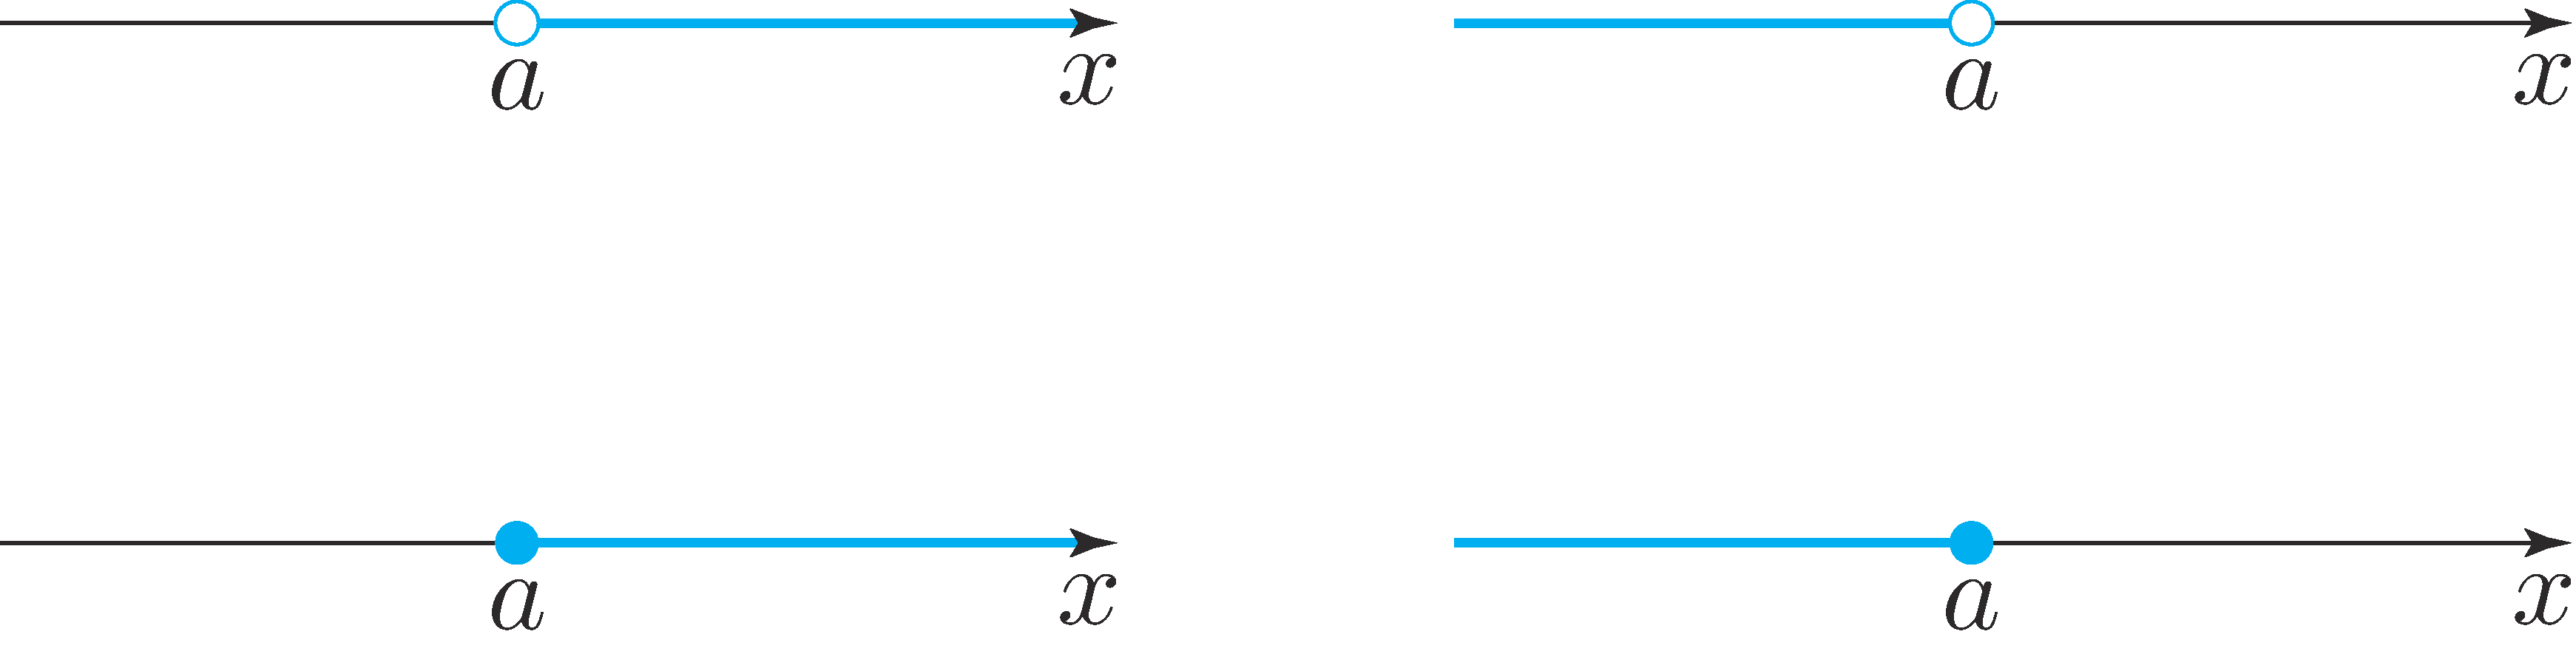
\includegraphics[scale=\pgfkeysvalueof{picsize}]{DBs/pic/zero_13.pdf}\
	\end{center}위 그림과 같이 범위의 한쪽 끝만 $a$로 제한되어 있을 때, $a$의 포함 여부에 따라 다음과 같이 $4$가지의 범위를 생각할 수 있습니다. %각각의 읽는 법은 따로 정해져 있지 않습니다.
\begin{align*}
    x  >  a, \: && x < a, \\
    x \ge a, \: && x \le a
\end{align*}\clearpage
$x>a$가 나타내는 구간의 왼쪽은 열려 있고, 구간의 왼쪽 끝은 $a$임이 확실합니다. 그러나 구간의 오른쪽 끝을 실수로 표기하기가 곤란합니다. 구간을 $\OCI{a}{b}$라고 표기하면, 이 표기는 부등식 $x>a$와 동일한 범위를 나타내지 않습니다. $c>b$인 실수 $c$가 존재하는데, $c$는 부등식 $x > a$의 해이지만, 구간 $\OCI{a}{b}$에는 포함되지 않기 때문입니다.\mn[-3\blskip]{이는 열린구간을 잡고 오른쪽 끝을 실수로 취했을 때에도 마찬가지입니다.}

이 실수 $c$를 포함하기 위하여 구간을 $\OCI{a}{c}$로 잡더라도 마찬가지입니다. $d>c$인 실수 $d$를 생각하면 모순이 발생하기 때문입니다. 이와 같이 부등식으로 나타낸 범위에 포함되는 모든 실수를 구간표기법으로 나타내려 하는 시도는 항상 실패할 수밖에 없습니다.\mn[-2\blskip]{잘 와닿지 않는다면 구체적인 숫자를 넣어 생각해보는 것이 좋습니다. 구간의 오른쪽 끝을 $1$억으로 잡으면 \mbox{$2$조를} 포함하지 못하고, \mbox{$2$조를} 포함하기 위해 구간의 오른쪽 끝을 $3$조로 잡으면 $10$조를 포함하지 못하는 것처럼, 어떤 실수를 잡더라도 더 큰 수가 존재하고, 그 수를 포함할 수 없습니다.}{}

따라서 $x>a$가 나타내는 범위를 표기하기 위하여 `그 어떤 실수보다도 큼'을 의미하는 기호인 $\infty$를 도입하고, $\OOI{a}{\infty}$라 표기합니다. 마찬가지로 $x \le a$가 나타내는 범위를 표기하기 위하여 `그 어떤 실수보다도 작음'을 의미하는 기호인  $-\infty$를 도입하고, $\OCI{-\infty}{a}$라 표기합니다. 그리고 $\infty$는 \term{무한대}{} 또는 \term{양의 무한대}{}, $-\infty$는 \term{음의 무한대}{}라 합니다.

주의할 점은, $\infty$와 $-\infty$는 절대로 실수가 아니라는 것입니다. 앞서 설명했듯 구간의 오른쪽 끝은 어떤 실수도 될 수 없으므로, $\infty$는 그 어떤 실수와도 같을 수 없습니다. 따라서 $\infty$는 실수가 아닙니다. $-\infty$ 또한 마찬가지입니다. 이를 달리 말하면, $\infty$와 $-\infty$는 $\mathbb{R}$의 원소가 아님에도 불구하고, $a \in \mathbb R$인 실수 $a$와 크기를 비교할 수 있는 특별한 개체\mn[2\blskip]{임의의 $a$에 대하여 $-\infty < a < \infty$입니다.}{}라 할 수 있습니다.

\subsection{실수 전체의 범위}
지금까지 설명한 내용을 바탕으로 생각하면, 실수 전체의 범위를 나타내기 위해서 구간의 왼쪽 끝과 구간의 오른쪽 끝을 각각 $-\infty$, $\infty$로 하여 $\OOI{-\infty}{\infty}$라 표기하는 것이 자연스럽습니다.

%\end{document}
\mychapter{여러 가지 식}{}
\section{등식}
등호와 수, 식을 이용하여 두 수, 수와 식, 식과 식이 서로 같음을 표현하는 식을 \term{등식}{}이라고 합니다.\mn{등식의 성질은 이 책에서 설명하지 않고 생략합니다.}{} 등식에는 항등식과 방정식이 있습니다. 방정식은 뒤에서 다루고, 먼저 항등식을 다루어 봅시다.
\subsection{항등식}
$x$에 대한 \term{항등식}{}은 식의 $x$에 대입할 수 있는 모든 실수 $x$에 대하여 항상 성립하는 등식입니다. 각 변이 $x$에 대한 다항식인 항등식을 정리하면 $0 = 0$꼴이 됩니다. 각 변이 $x$에 대한 다항식인 어떤 등식이 항등식이라면 각 변에서 차수가 같은 항의 계수가 서로 같음을 이용하거나, 식을 간단히 만드는 적당한 값을 대입하여 풀이하면 됩니다.


\section{다항식의 연산}
덧셈, 뺄셈, 곱셈(전개)의 방법에 대한 서술은 생략합니다. 이 방법을 모른다면 이 책을 공부하기를 권하지 않습니다.

\subsection{곱셈 공식과 인수분해 공식}
좌변에서 우변을 얻는 것이 \term{곱셈 공식}{}, 우변에서 좌변을 얻는 것이 \term{인수분해 공식}{}입니다.

\begin{enumerate}[label=\onum*]
    \item $(a+b)^2 = a^2 + 2ab + b^2$

    \item $(a-b)^2 = a^2 - 2ab + b^2$
    \item $(a+b)(a-b) = a^2 - b^2$
    \item $(x+a)(x+b)=x^2 + (a+b)x+ab$
    \item $(ax+b)(cx+d)=acx^2 + (ad+bc)x + bd$
    \item $(a+b)^3 = a^3 + 3a^2b + 3ab^2 + b^3$
    \item $(a-b)^3 = a^3 - 3a^2b + 3ab^2 - b^3$
    \item $(a+b)(a^2-ab+b^2) = a^3  + b^3$
    \item $(a-b)(a^2+ab+b^2)=a^3 - b^3$
    \item $(a+b+c)^2 = a^2 + b^2 + c^2 + 2ab + 2bc + 2ca$
\end{enumerate}\cleartorecto

\subsection{다항식의 나눗셈부터 인수정리까지}
앞서와 마찬가지로 나눗셈의 방법과 조립제법에 대한 서술은 생략합니다.
\subsubsection{나눗셈에 대한 항등식}
다항식 $A$를 $0$이 아닌 다항식 $B$로 나누었을 때의 몫을 $Q$, 나머지를 $R$라고 하면 다음이 성립합니다. \begin{align*} A=BQ+R \quad \text{ (단, $R$의 차수는 $B$의 차수보다 낮음)} \end{align*}
\subsubsection{나머지정리}
나눗셈에 대한 항등식을 이용하여 다항식 $f\left( x \right) $를 일차식 $x-a$로 나누었을 때의 몫을 $Q\left( x \right) $, 상수인 나머지를 $r$라고 하면 다음이 성립합니다. \begin{align*} f\left( x \right) =\left( x-a \right)Q\left( x \right)  +r\end{align*}
이때 양변에 $x=a$를 대입하면 $f\left( a \right) = r$입니다. 이를 \term{나머지정리}{}라고 합니다.

나머지정리는 `다항함수의 함숫값을 해석하는 새로운 관점'을 제시한다는 점에서 의미를 가집니다. 예를 들어, 기존에는 다항함수 $f\left( x \right) $의 함숫값 $f\left( 3 \right) $을 구하기 위해서는 다항식에 포함된 각 항에 $x=3$을 대입하여 그 값을 계산해야 했고, 그 값에서 특별한 의미를 찾기 힘들었습니다. 그러나 이제는 나머지를 이용해 다른 함수를 $y$축 방향으로 평행이동한 것으로 해석할 수 있습니다. 이는 함수의 극한이나 미적분과 연계되어 다양한 해석과 풀이의 실마리를 제공하기도 합니다.

\subsubsection{인수정리}
나머지정리에서 $r=0$이면, 즉 $f\left( a \right) =0$이면 $f(x)$가 $x-a$로 나누어떨어집니다. 반대로, $f(x)$가 $x-a$로 나누어떨어지면 $r=0$이므로 $f\left( a \right) =0$입니다. 이를 \term{인수정리}{}라 합니다.

인수정리는 `다항식을 세련된 방식으로 인수분해하는 방법'을 제시한다는 점에서 의미를 가집니다. 이 또한 함수의 극한이나 미적분과 연계되어 다양한 해석과 풀이의 실마리를 제공하기도 합니다.
\clearpage
\section{방정식}
$x$의 값에 따라 참이 되기도 하고 거짓이 되기도 하는 $x$에 대한 등식을 방정식이라고 합니다. 이때 $x$를 \term{미지수}{}라 하며, 이 방정식을 참이 되게 하는 $x$를 \term{해}{} 또는 \term{근}{}이라고 합니다.

\subsection{일차방정식}
미지수에 대한 일차 다항식으로 구성된 방정식을 \term{일차방정식}{}이라고 합니다. 적절히 이항하여 근을 구할 수 있습니다.

\subsection{이차방정식의 근과 판별식}
미지수에 대한 이차 다항식으로 구성된 방정식을 \term{이차방정식}{}이라고 합니다. 각 항의 계수가 실수인 이차방정식 $ax^2 + bx + c=0\: (a\ne 0)$의  두 근은 다음과 같습니다.
\begin{align*} x= \dfrac{-b\pm\sqrt{b^2-4ac}}{2a} \end{align*}
이때 $b^2 - 4ac \ge 0$이면 $\sqrt{b^2 - 4ac}$는 실수이고, $b^2 - 4ac < 0$이면 허수\mn{허수 및 복소수는 교육과정 미적분에서 비중이 매우 떨어지므로 Zero에 수록하지 않았습니다.}{}입니다. 따라서 계수가 실수인 이차방정식은 복소수의 범위에서 반드시 근을 가지며, 실수인 근을 \term{실근}{}, 허수인 근을 \term{허근}{}이라고 합니다. 이와 같이 $b^2 - 4ac$는 이차방정식의 근을 판별해주는 역할을 하므로 \term{판별식($D$)}{}이라 합니다.

\subsection{고차방정식과 연립방정식}
미지수에 대한 삼차 이상의 다항식으로 구성된 방정식을 \term{고차방정식}{}이라 합니다. 인수분해가 가능한 식은 인수분해하여 풀이할 수 있습니다. 그렇지 않은 고차방정식은 미분을 배운 후 제한적으로 풀이할 수 있습니다.

둘 이상의 방정식을 연립한 것을 \term{연립방정식}{}이라고 합니다. 연립방정식은 대입/가감 등을 이용하여 미지수를 적절히 소거하여 풀이합니다.
\clearpage
\section{부등식}
부등호 $<$, $>$, $\le$, $\ge$을 이용하여 두 수, 수와 식, 식과 식의 크기를 비교하는 식을 \term{부등식}{}이라고 합니다. 어떤 부등식이 마치 방정식처럼 $x$의 값에 따라 참이 되기도 하고 거짓이 되기도 할 때, 그 부등식을 `\term{$x$에 대한 부등식}{}'이라고 합니다. 이때 $x$를 \term{미지수}{}라 하며, 이 부등식을 참이 되게 하는 $x$를 \term{해}{}라고 합니다.\mn{방정식에서는 근과 해가 두루 쓰이지만, 부등식에서는 근이라는 표현을 거의 쓰지 않습니다.}{}

\subsection{일차부등식}
적절히 이항하여 해를 구할 수 있습니다. 

\subsection{이차부등식의 근과 판별식}
이차부등식의 풀이는 단순 암기에 그치면 안 되고, 수식과 그래프를 넘나드는 복합적 이해를 통해 숙지해야 합니다. 따라서 Graph 0)에서 다룹니다.

\subsection{고차부등식과 연립부등식}
삼차 이상의 부등식을 \term{고차부등식}{}이라 합니다. 인수분해가 가능한 식은 인수분해하여 풀이할 수 있습니다. 그렇지 않은 고차부등식은 미분을 배운 후 제한적으로 풀이할 수 있습니다.

둘 이상의 부등식을 연립한 것을 \term{연립부등식}{}이라고 합니다. 연립부등식은 각각의 부등식의 해를 구한 후, 모든 부등식의 공통해를 취하여 풀이합니다.


\mychapter{명제}{}

\section{명제}
참인지 거짓인지를 분명하게 판별할 수 있는 문장이나 식을 \term{명제}{}라고 합니다. 예를 들어 `$6$은 $2$의 배수이다'라는 문장과 $2 - 4 = 0$이라는 식은 명제입니다.

\section{조건}
`$x$는 $2$의 배수이다'라는 문장과 $x-4 = 0$이라는 식은 그 자체로는 명제가 아니지만, $x$의 값에 $4$를 대입하면 각각 참, 참이고, $x$의 값에 $6$을 대입하면 각각 참, 거짓이고, $x$의 값에 $5$를 대입하면 각각 거짓, 거짓입니다. 이와 같이 변수를 포함하는 문장이나 식이 변수의 값에 따라 참인지 거짓인지 결정될 때, 이러한 문장이나 식을 \term{조건}{}이라고 합니다.

\subsection{조건의 진리집합}
어떤 전체집합 $U$가 주어졌을 때, $U$의 원소 중에서 $p$라는 조건을 참이 되도록 하는 원소의 집합을 조건 $p$의 진리집합이라고 합니다. 집합의 조건제시법에서, 조건 $p$를 제시했을 때 얻는 집합이 바로 진리집합입니다.

\section{명제의 부정}
명제 $p$에 대하여 `$p$가 아니다'라는 명제를 `명제 $p$의 부정'이라고 하며 $\sim p$라 표기합니다. $p$가 참이면 $\sim p$는 거짓이고, $p$가 거짓이면 $\sim p$는 참입니다.

조건 $q$에 대하여 `$q$가 아니다'라는 조건을 `조건 $q$의 부정'이라고 하며 $\sim q$라 표기합니다. 전체집합 $U$에 대하여 $q$의 진리집합이 $Q$이면 $\sim q$의 진리집합은 $Q^C$입니다.

\section{`모든'과 `어떤'}

\subsection{`모든'을 포함한 명제}
`모든 $x$에 대하여 $p$이다'가 참이라는 것은 전체집합 $U$의 모든 원소 $x$에 대하여 조건 $p$가 참이라는 것(조건을 만족시킨다는 것)을 뜻합니다. `모든 $x$에 대하여 $p$이다'가 거짓이라는 것은 전체집합 $U$의 원소 중 조건 $p$를 참이 되게 하지 않는 원소가 적어도 하나 존재한다는 것을 뜻합니다. 따라서 조건 $p$의 진리집합이 $P$일 때, $P=U$이면 주어진 명제가 참이고, $P \ne U$이면 주어진 명제가 거짓입니다.

\subsection{`어떤'을 포함한 명제}
`어떤 $x$에 대하여 $p$이다'가 참이라는 것은 전체집합 $U$의 원소 중 조건 $p$를 참이 되게 하는 원소가 적어도 하나 존재한다는 것을 뜻합니다. `어떤 $x$에 대하여 $p$이다'가 거짓이라는 것은 전체집합 $U$의 원소 중 조건 $p$가 참이 되게 하는 원소가 하나도 존재하지 않는다는 것을 뜻합니다. 따라서 조건 $p$의 진리집합이 $P$일 때, $P \ne \emptyset$이면 주어진 명제가 참이고, $P =\emptyset$이면 주어진 명제가 거짓입니다.
\cleartorecto
\subsection{`모든'과 `어떤'의 관계}
`모든 $x$에 대하여 $p$이다'의 부정은 `어떤 $x$에 대하여 $\sim p$이다'이고, `어떤 $x$에 대하여 $p$이다'의 부정은 `모든 $x$에 대하여 $\sim p$이다'입니다.


\section{가정과 결론으로 구성된 명제}
진리집합이 각각 $P$, $Q$인 두 조건 $p$와 $q$를 `$p$이면 $q$이다.'의 꼴로 연결한 명제를 $p \longrightarrow q$라 표기하고, $p$를 가정, $q$를 결론이라고 합니다. $p \longrightarrow q$가 참이면 $P \subset Q$입니다. 반대로 $P \subset Q$이면 $p \longrightarrow q$는 참입니다.  $p \longrightarrow q$가 거짓이면 $P \not\subset Q$입니다. 반대로 $P \not\subset Q$이면 $p \longrightarrow q$는 거짓입니다.

\subsection{명제의 역과 대우}
명제 $q \longrightarrow p$를 $p \longrightarrow q$의 역이라 합니다. 명제 $\sim q \longrightarrow \sim p$를 $p \longrightarrow q$의 대우라고 합니다. 명제가 참이면 대우도 참입니다.\mn{진리집합의 포함관계를 통해 알 수 있습니다.}{} 명제가 참이라고 해서 역이 참인 것은 아닙니다(참인 경우도 있고, 거짓인 경우도 있습니다).

\section{정의, 증명, 정리}
용어의 뜻을 명확하게 정한 문장을 정의라 합니다. 정의 혹은 이미 알려진 사실이나 성질을 이용하여 명제가 참 또는 거짓임을 밝히는 과정을 증명이라고 합니다. 또한 참으로 증명된 명제 중에서 기본이 되는 것, 여러 가지 성질을 증명할 때 자주 이용되는 것을 정리라고 합니다. 어떤 명제를 증명할 때에는 명제를 가정과 결론으로 나누어 생각하면 편리합니다.

\subsection{대우를 이용한 증명법}
명제를 증명하기 어려운 경우, 대우를 이용하여 증명하면 편리한 경우가 있습니다.

\subsection{귀류법}
가정에서 결론을 직접 이끌어내기 어렵지만, 명제를 부정하면 모순이 발생함을 보이는 것은 쉬운 경우가 있습니다. 이와 같이 명제의 부정에서 모순을 이끌어내어 원래 명제가 참임을 보이는 증명 방법을 \term{귀류법}{}이라고 합니다.

\section{필요조건과 충분조건}
$p \longrightarrow q$가 참이면 $p \Longrightarrow q$라 표기합니다. 이때 $p$는 $q$이기 위한 충분조건, $q$는 $p$이기 위한 필요조건이라고 합니다. 

$p \Longrightarrow q$이고 $q \Longrightarrow p$일 때, $p \Longleftrightarrow q$라 표기하고, $p$는 $q$이기 위한 필요충분조건이라고 합니다. 이때 두 조건의 진리집합은 서로 같습니다. 




\mychapter{평면좌표}{}
\section{좌표평면}
\begin{center}
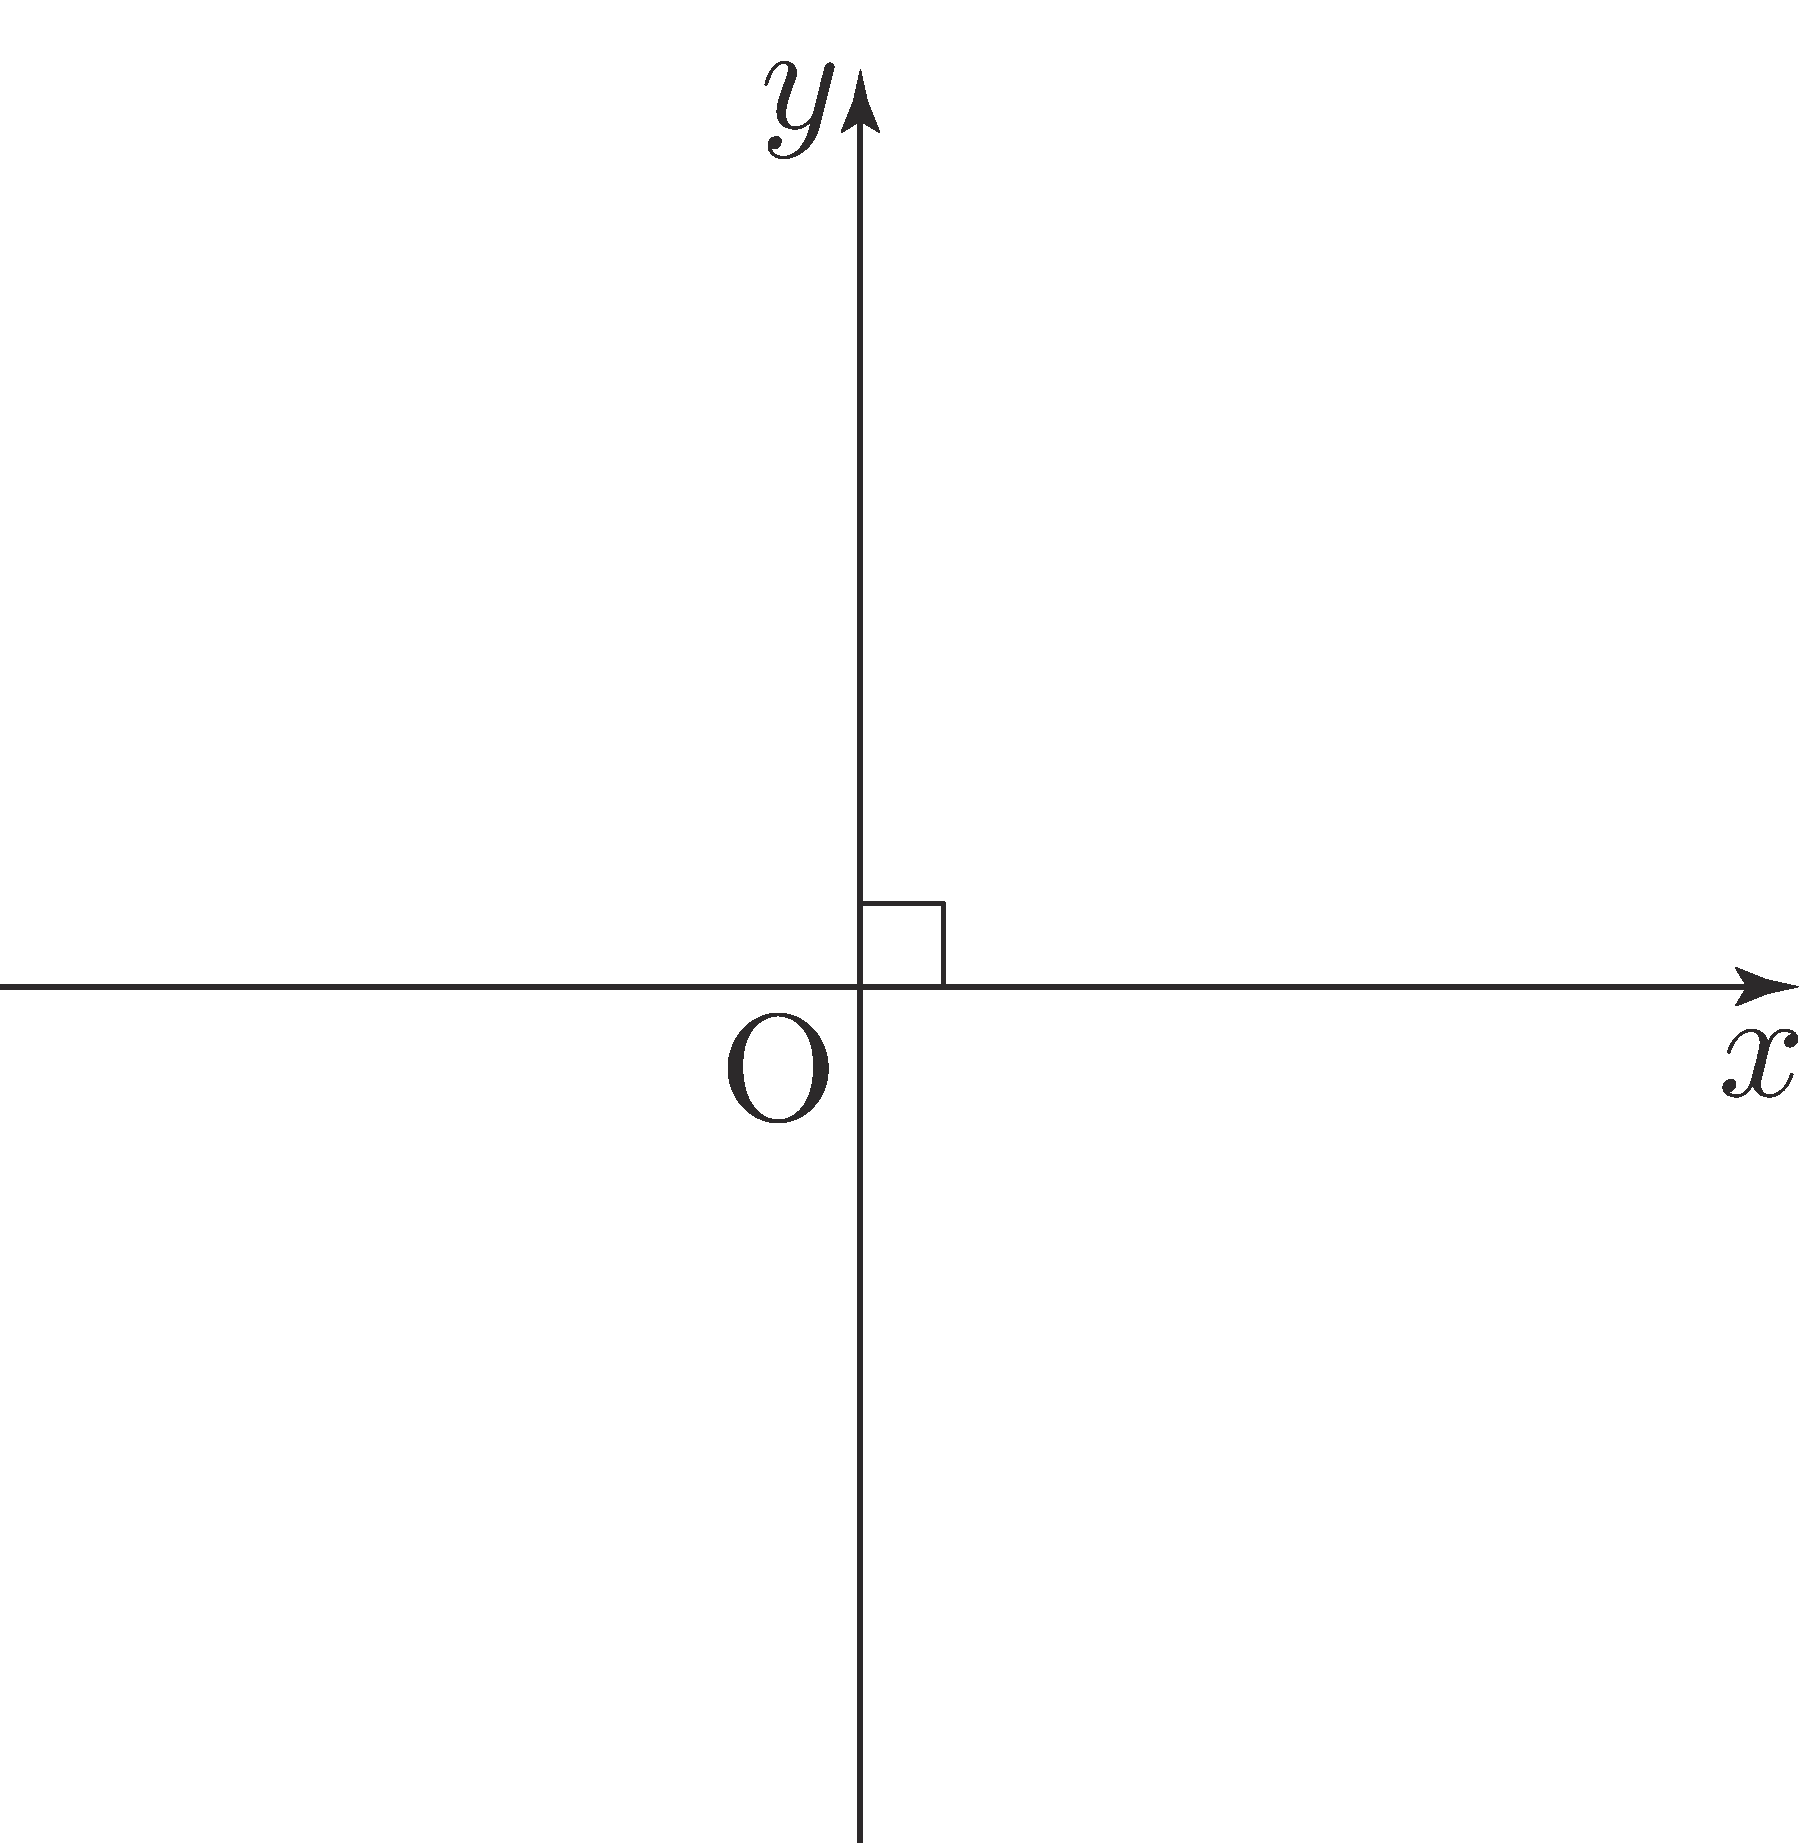
\includegraphics[scale=0.125]{pic0/pic142.pdf}
\end{center}평면의 한 점 $\mrm{O}$에서 서로 직교하는 두 수직선을 그어 각각 $x$축, $y$축이라 하고, 이들을 통틀어 \term[좌표축]{좌표평면에서의 좌표축}{1}이라고 합니다. 이때 점 $\mrm{O}$를 \term[원점]{좌표평면}{1}이라고 합니다. 이와 같이 좌표축이 정해진 평면을 \term{좌표평면}{}이라고 합니다.
\section{평면좌표}
\begin{center}
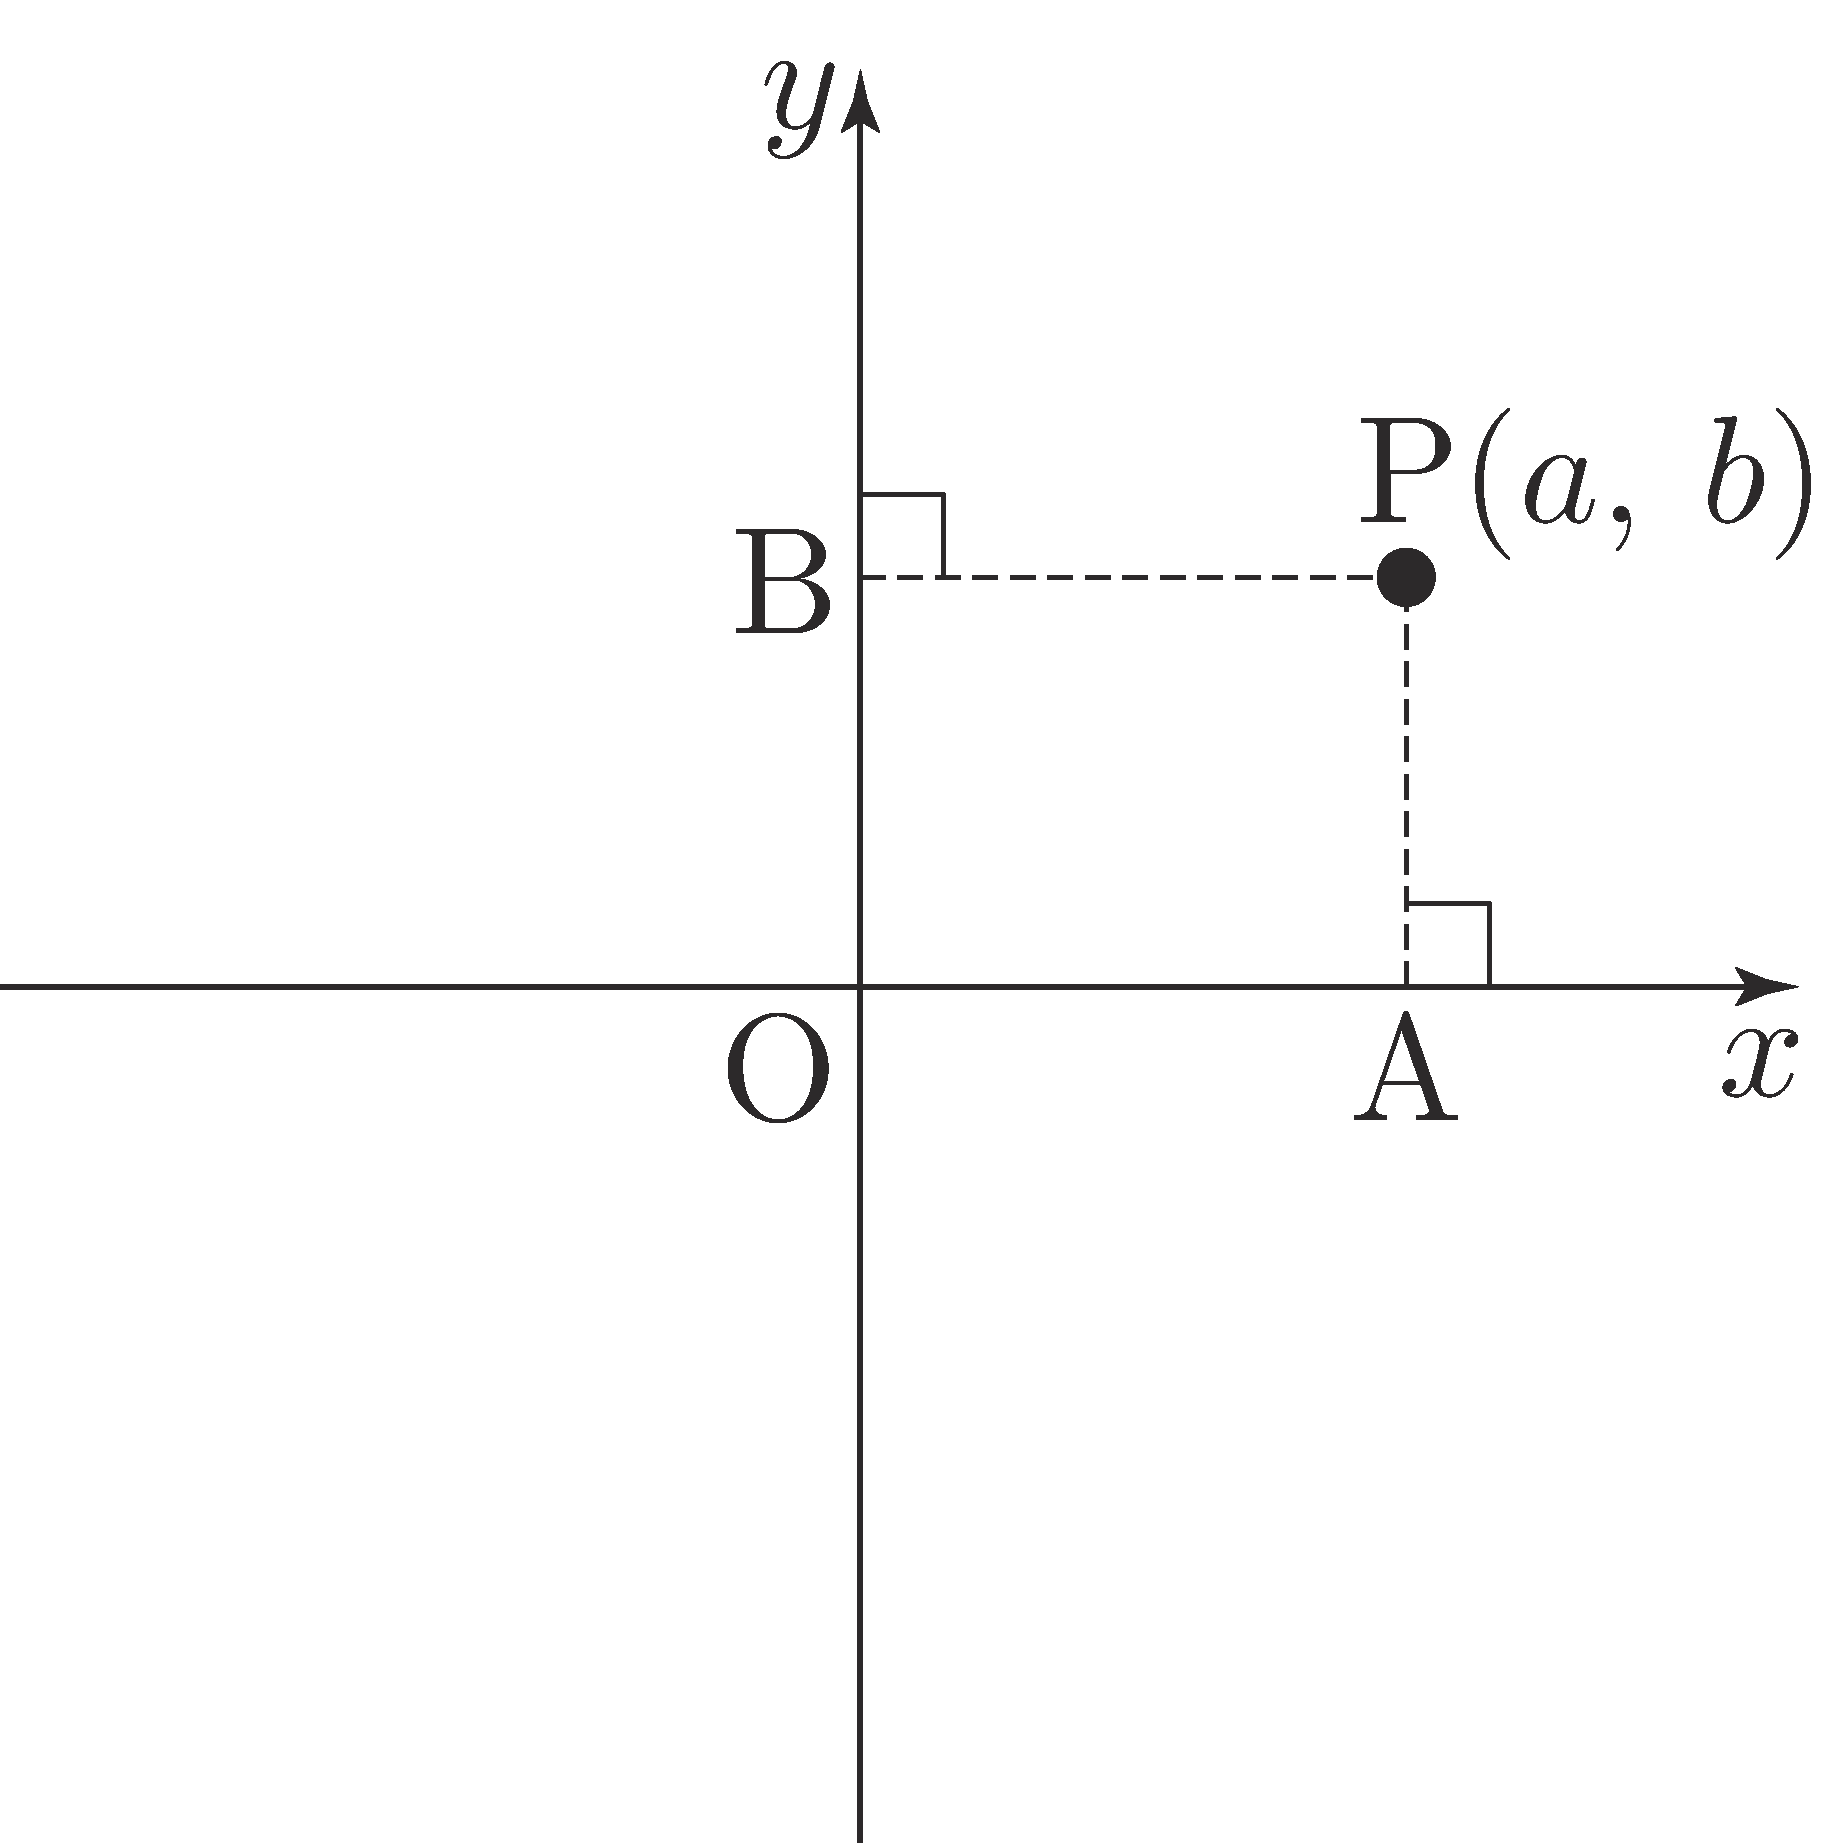
\includegraphics[scale=0.125]{pic0/pic143.pdf}
\end{center}좌표평면의 한 점 $\mrm{P}$에 대하여 점 $\mrm{P}$를 지나고 $x$축, $y$축에 각각 수직인 직선이 이들 축과 만나는 점을 차례로 $\mrm{A}$, $\mrm{B}$라고 하겠습니다. 이때 두 점 $\mrm{A}$, $\mrm{B}$의 $x$축, \mbox{$y$축} 위에서의 좌표를 각각 $a$, $b$라 하면
점 $\mrm{P}$에 대응하는 두 실수의 순서쌍 $\xy{a}{b}$가 정해집니다. 반대로 두 실수의 순서쌍 $\xy{a}{b}$가 주어지면 평면에 있는 한 점 $\mrm{P}$를 대응시킬 수 있습니다.

따라서 평면의 점 $\mrm{P}$와 두 실수의 순서쌍 $\xy{a}{b}$는 일대일로 대응되므로 점 $\mrm{P}$에 대응하는 이 순서쌍을 점 $\mrm{P}$의 \term{평면좌표}{}라 하고, $a$, $b$를 각각 점 $\mrm{P}$의 \term{$x$좌표}{}, \term{$y$좌표}{}라 합니다. 또한 점 $\mrm{P}$의 좌표가 $\xy{a}{b}$일 때 $\xy[P]{a}{b}$라 표기합니다.

\cleartorecto

\term[거리!좌표평면]{두 점 사이의 거리}{0}
\section{두 점 사이의 거리}
{\color{white}.}\\[-1.55\blskip]\begin{center}
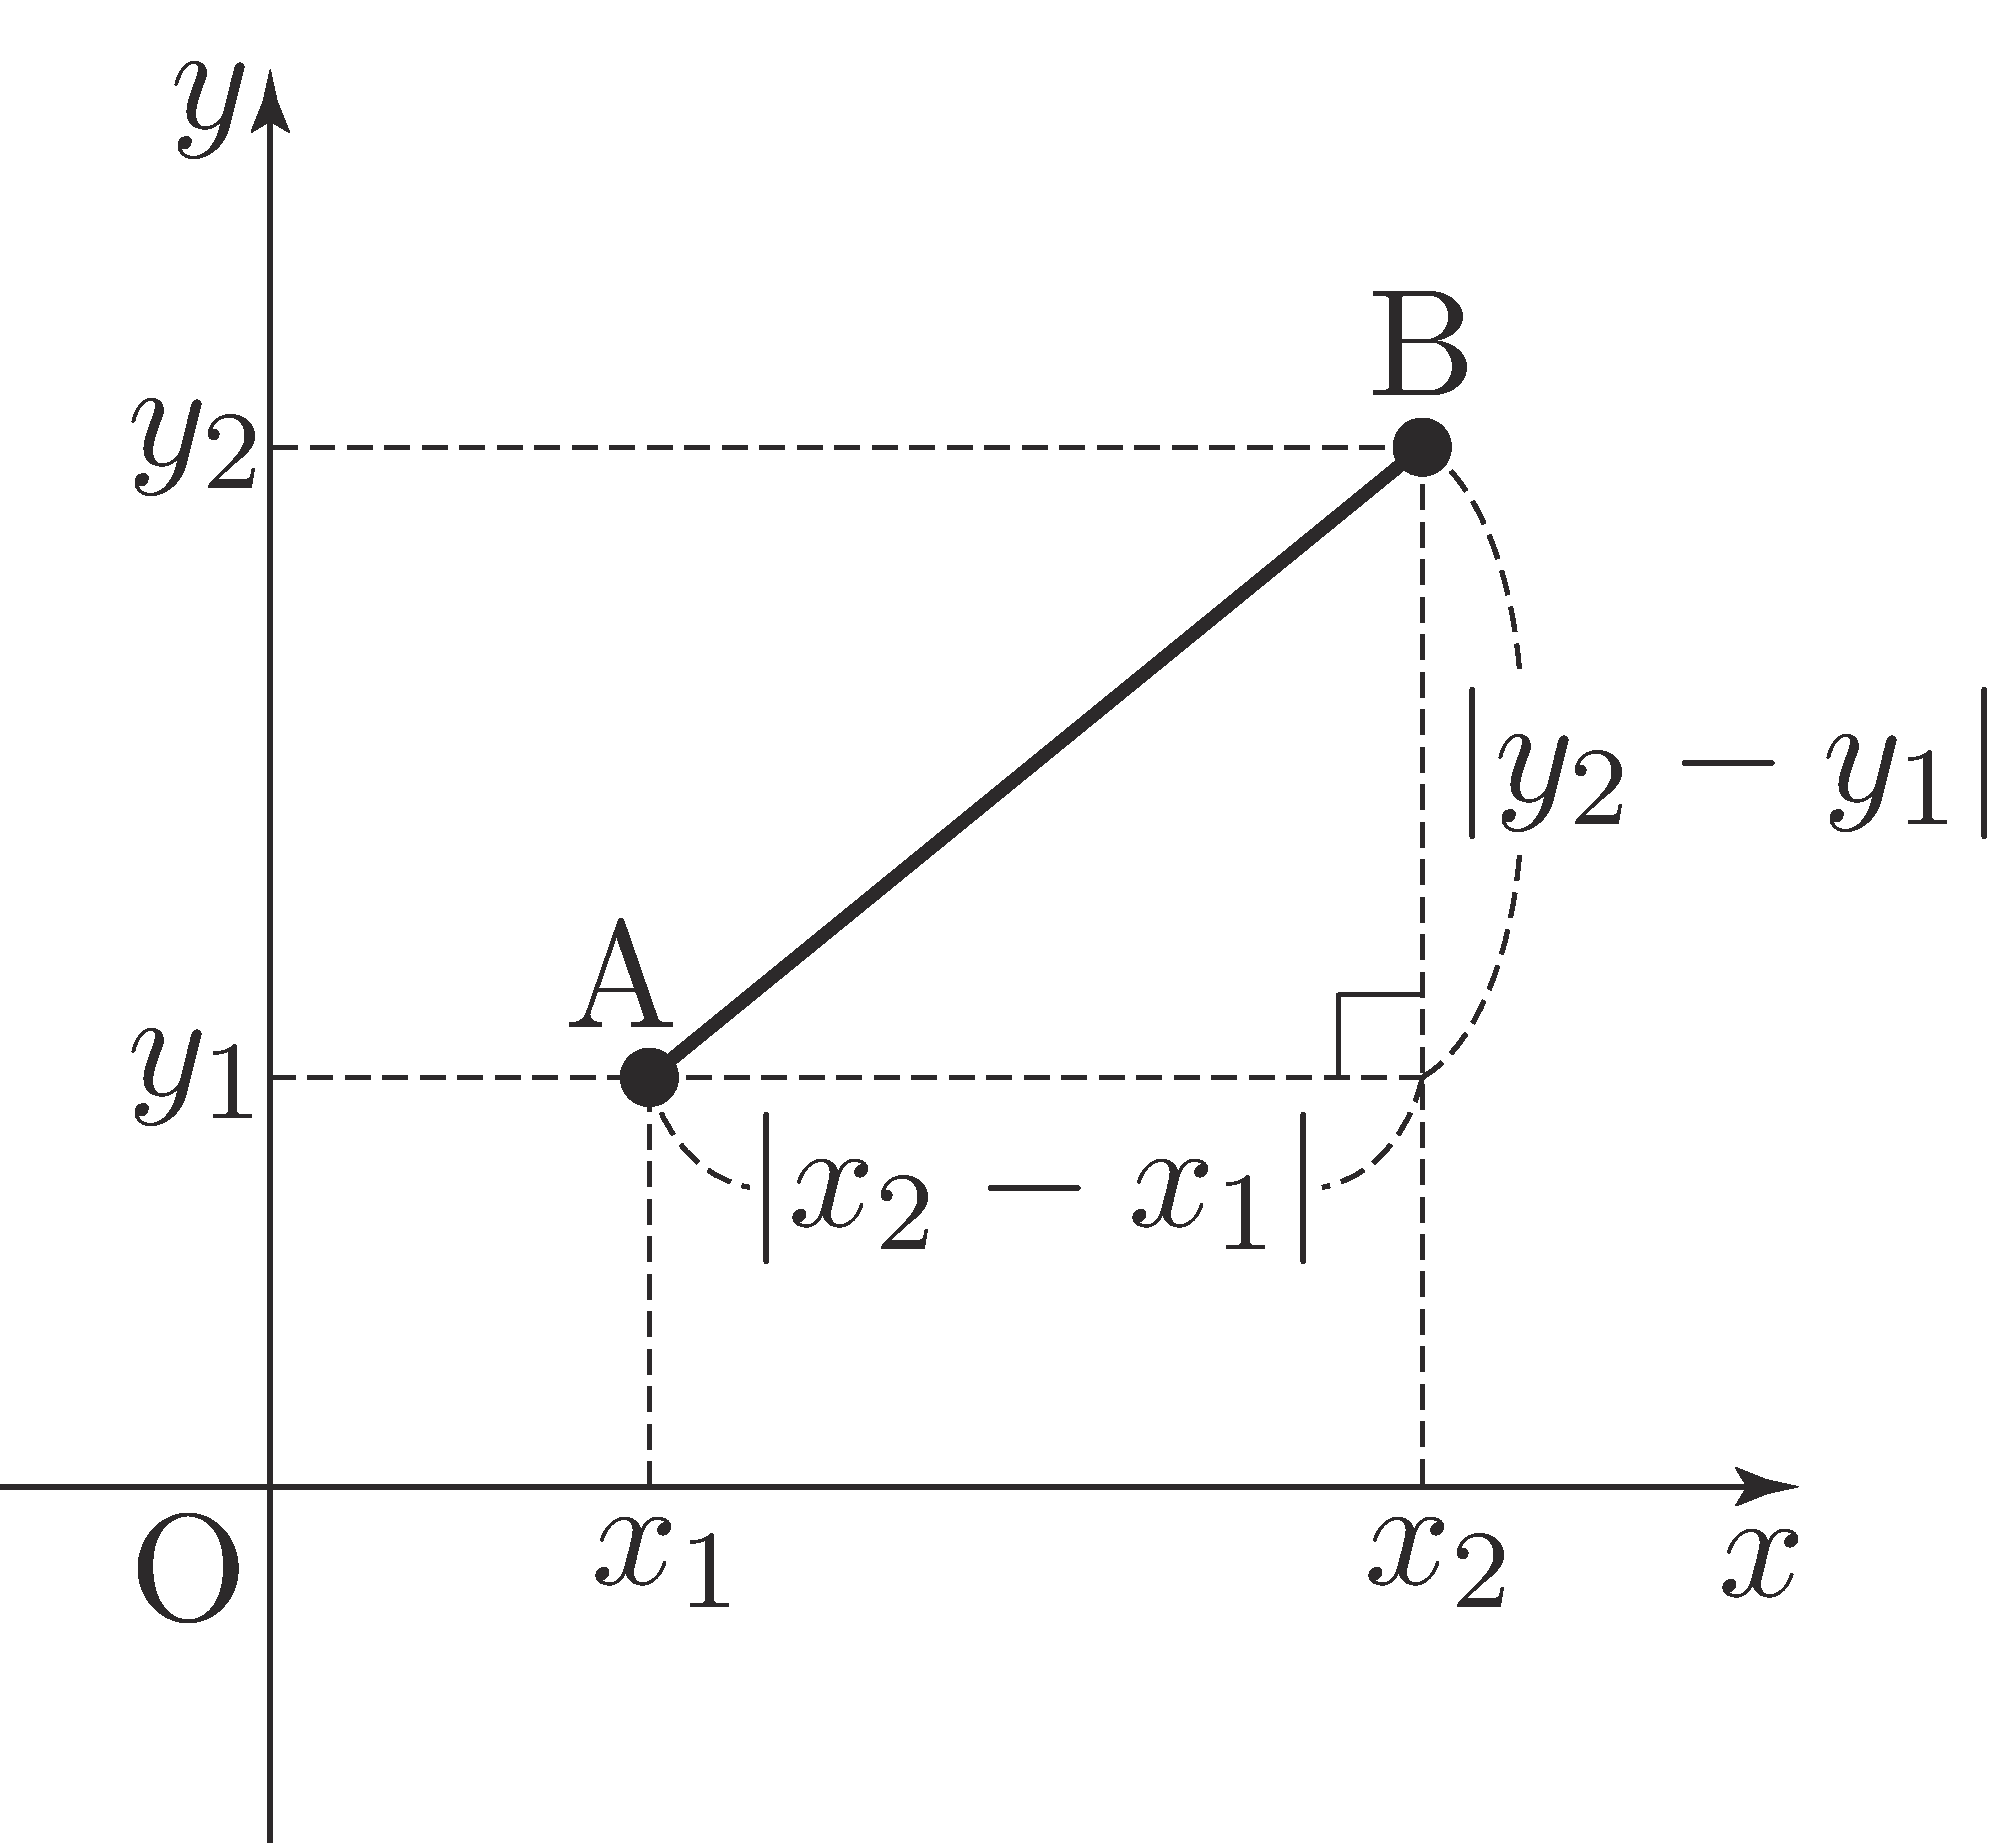
\includegraphics[scale=0.125]{pic0/pic144.pdf}\
\end{center}좌표평면에서 두 점 $\xy[A]{x_1}{y_1}$, $\xy[B]{x_2}{y_2}$ 사이의 거리 $\ovr{AB}$는 다음과 같습니다. \begin{align*}\ovr{AB} = \sqrt{(x_2 - x_1)^2 + (y_2 - y_1)^2}\end{align*}\\[-4.5em]
\section{내분점과 외분점}\term[내분]{좌표평면에서의 내분}{0}\term[외분]{좌표평면에서의 내분}{0}
\begin{center}
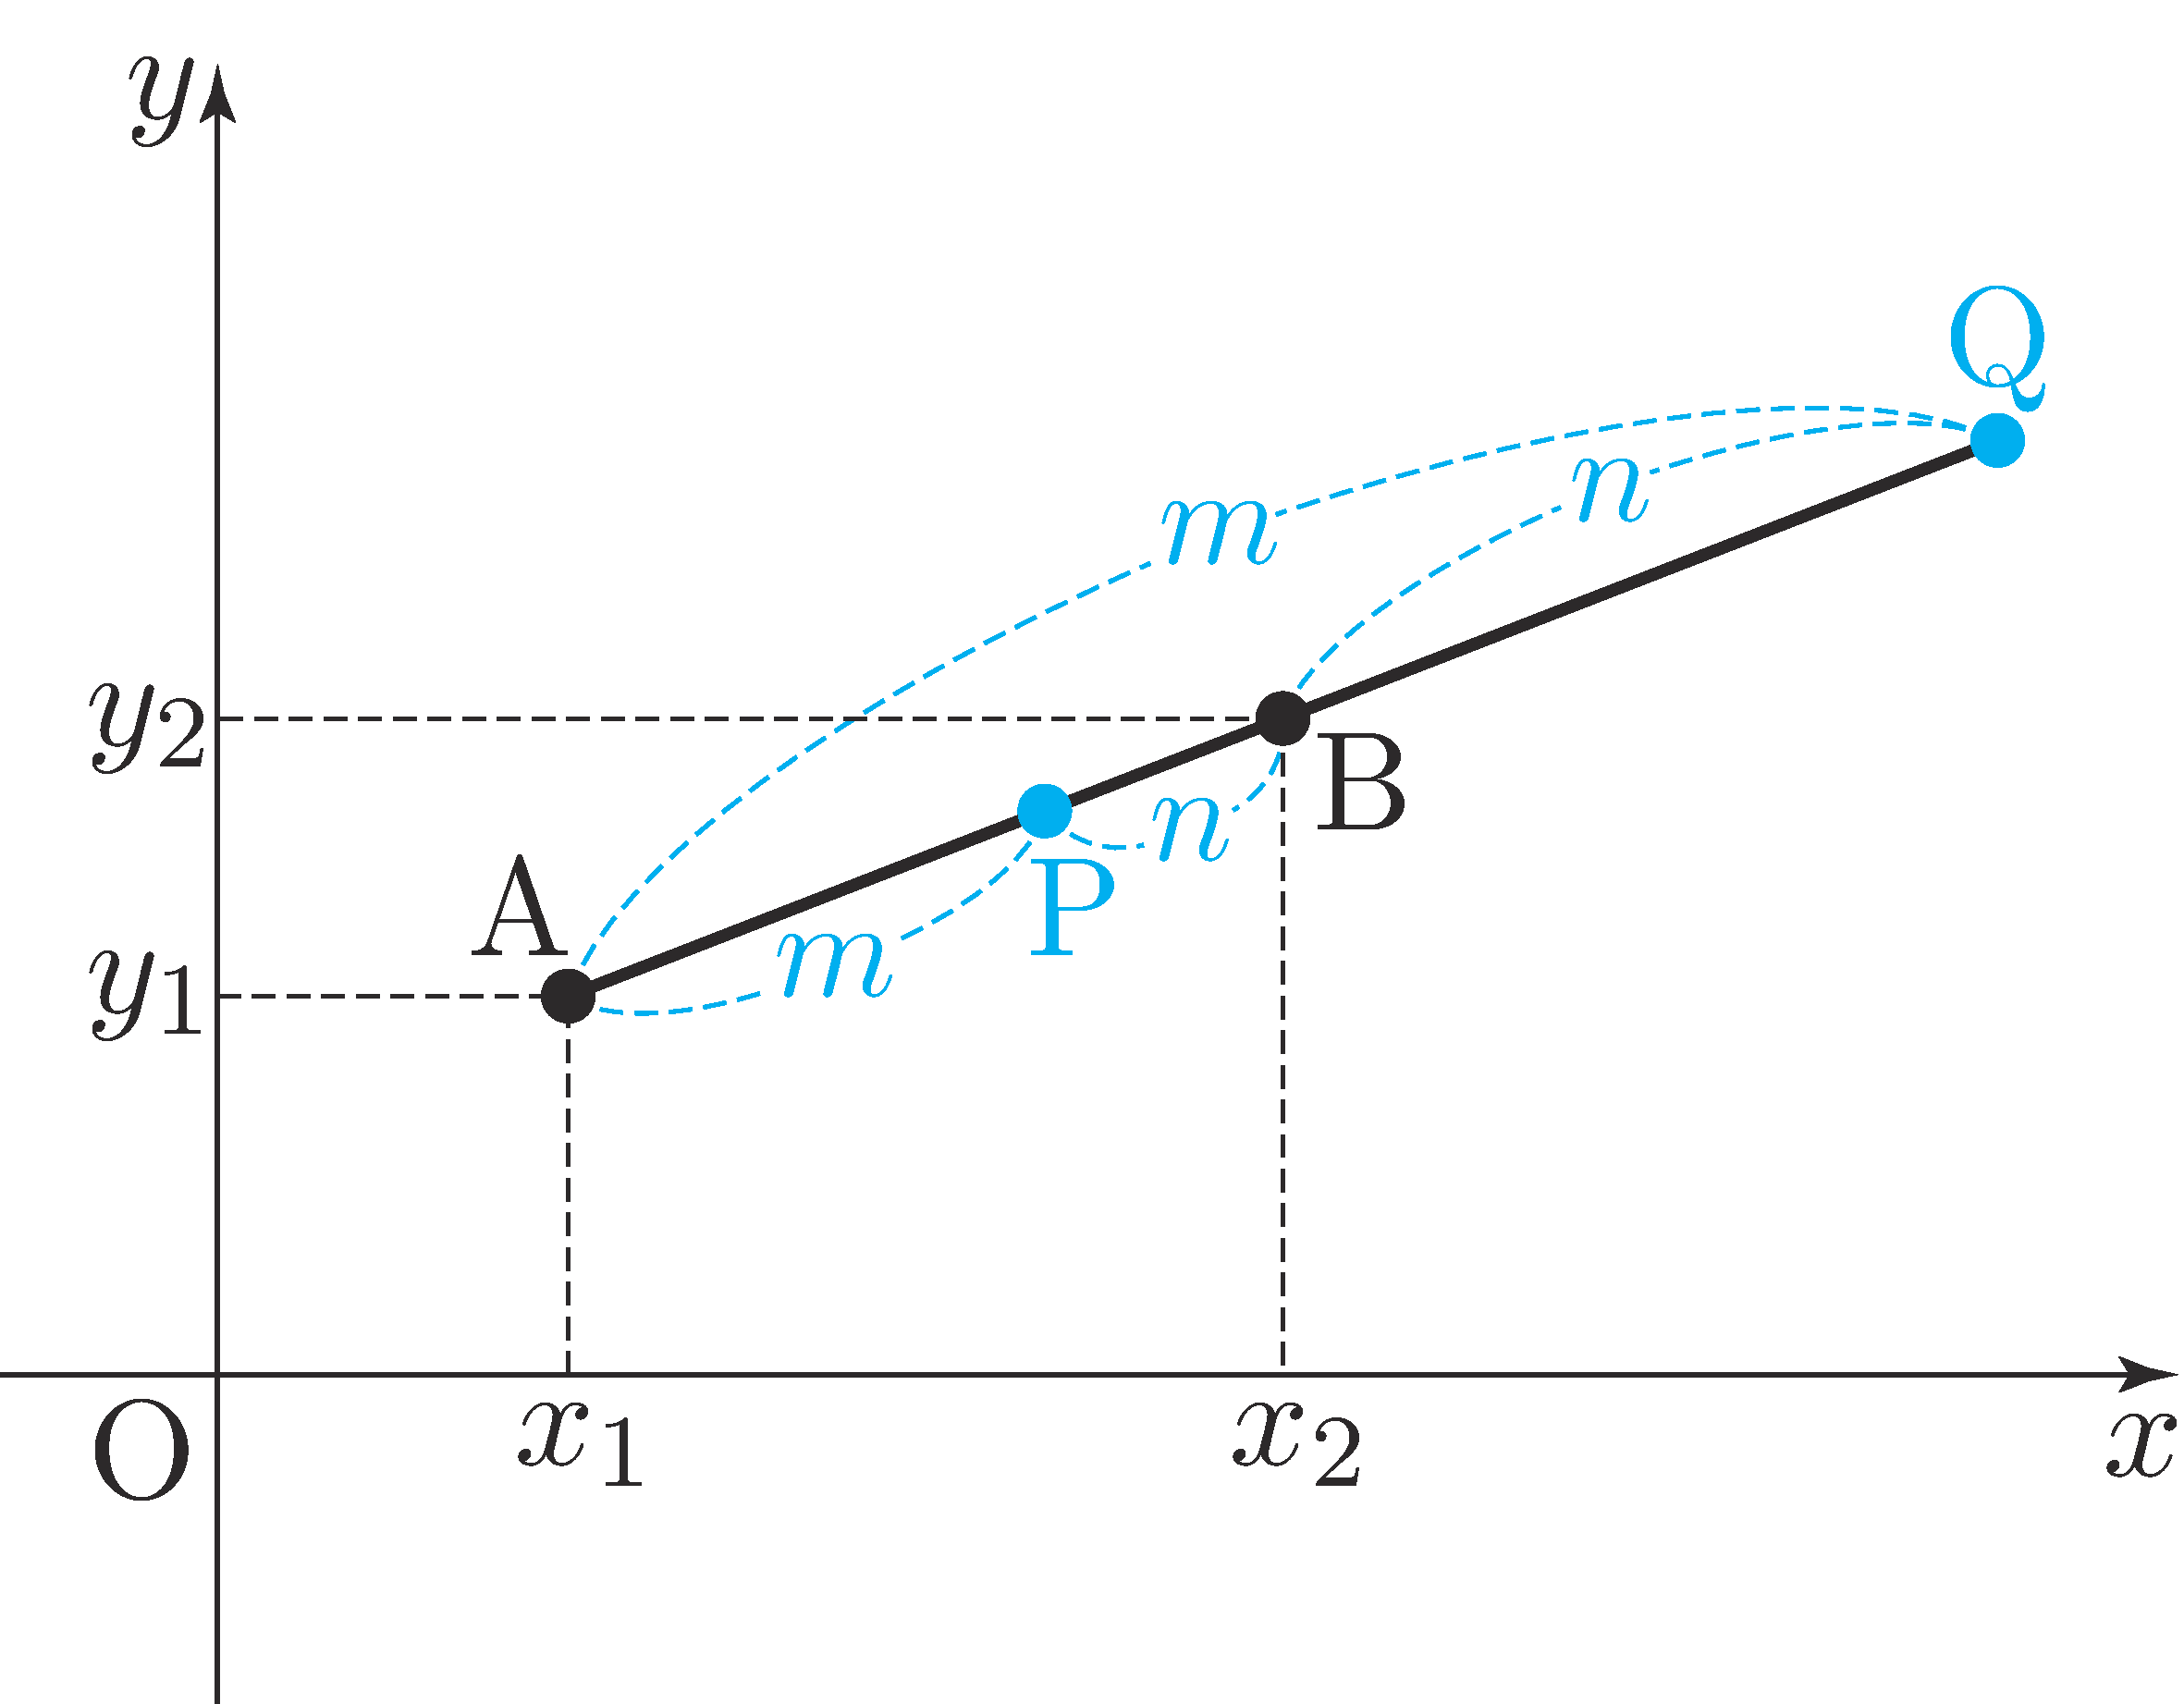
\includegraphics[scale=0.125]{pic0/pic145.pdf}\
\end{center}좌표평면에서 두 점 $\xy[A]{x_1}{y_1}$, $\xy[B]{x_2}{y_2}$에 대하여 선분 $\mrm{AB}$를 $m:n$으로 내분하는 점 $\mrm{P}$의 좌표와 $m:n$으로 외분하는 점 $\mrm{Q}$의 좌표는 각각 다음과 같습니다.\mn{외분할 때에는 $m\ne n$이어야 합니다.}{}\\[-1em]
\begin{align*}
  \xy[P]{\IDP{x_1}{x_2}{m}{n}}{\IDP{y_1}{y_2}{m}{n}},\quad
  \xy[Q]{\EDP{x_1}{x_2}{m}{n}}{\EDP{y_1}{y_2}{m}{n}}
\end{align*}\\[-4.5em]
\section{무게중심}\term[무게중심]{좌표평면}{0}
\begin{center}
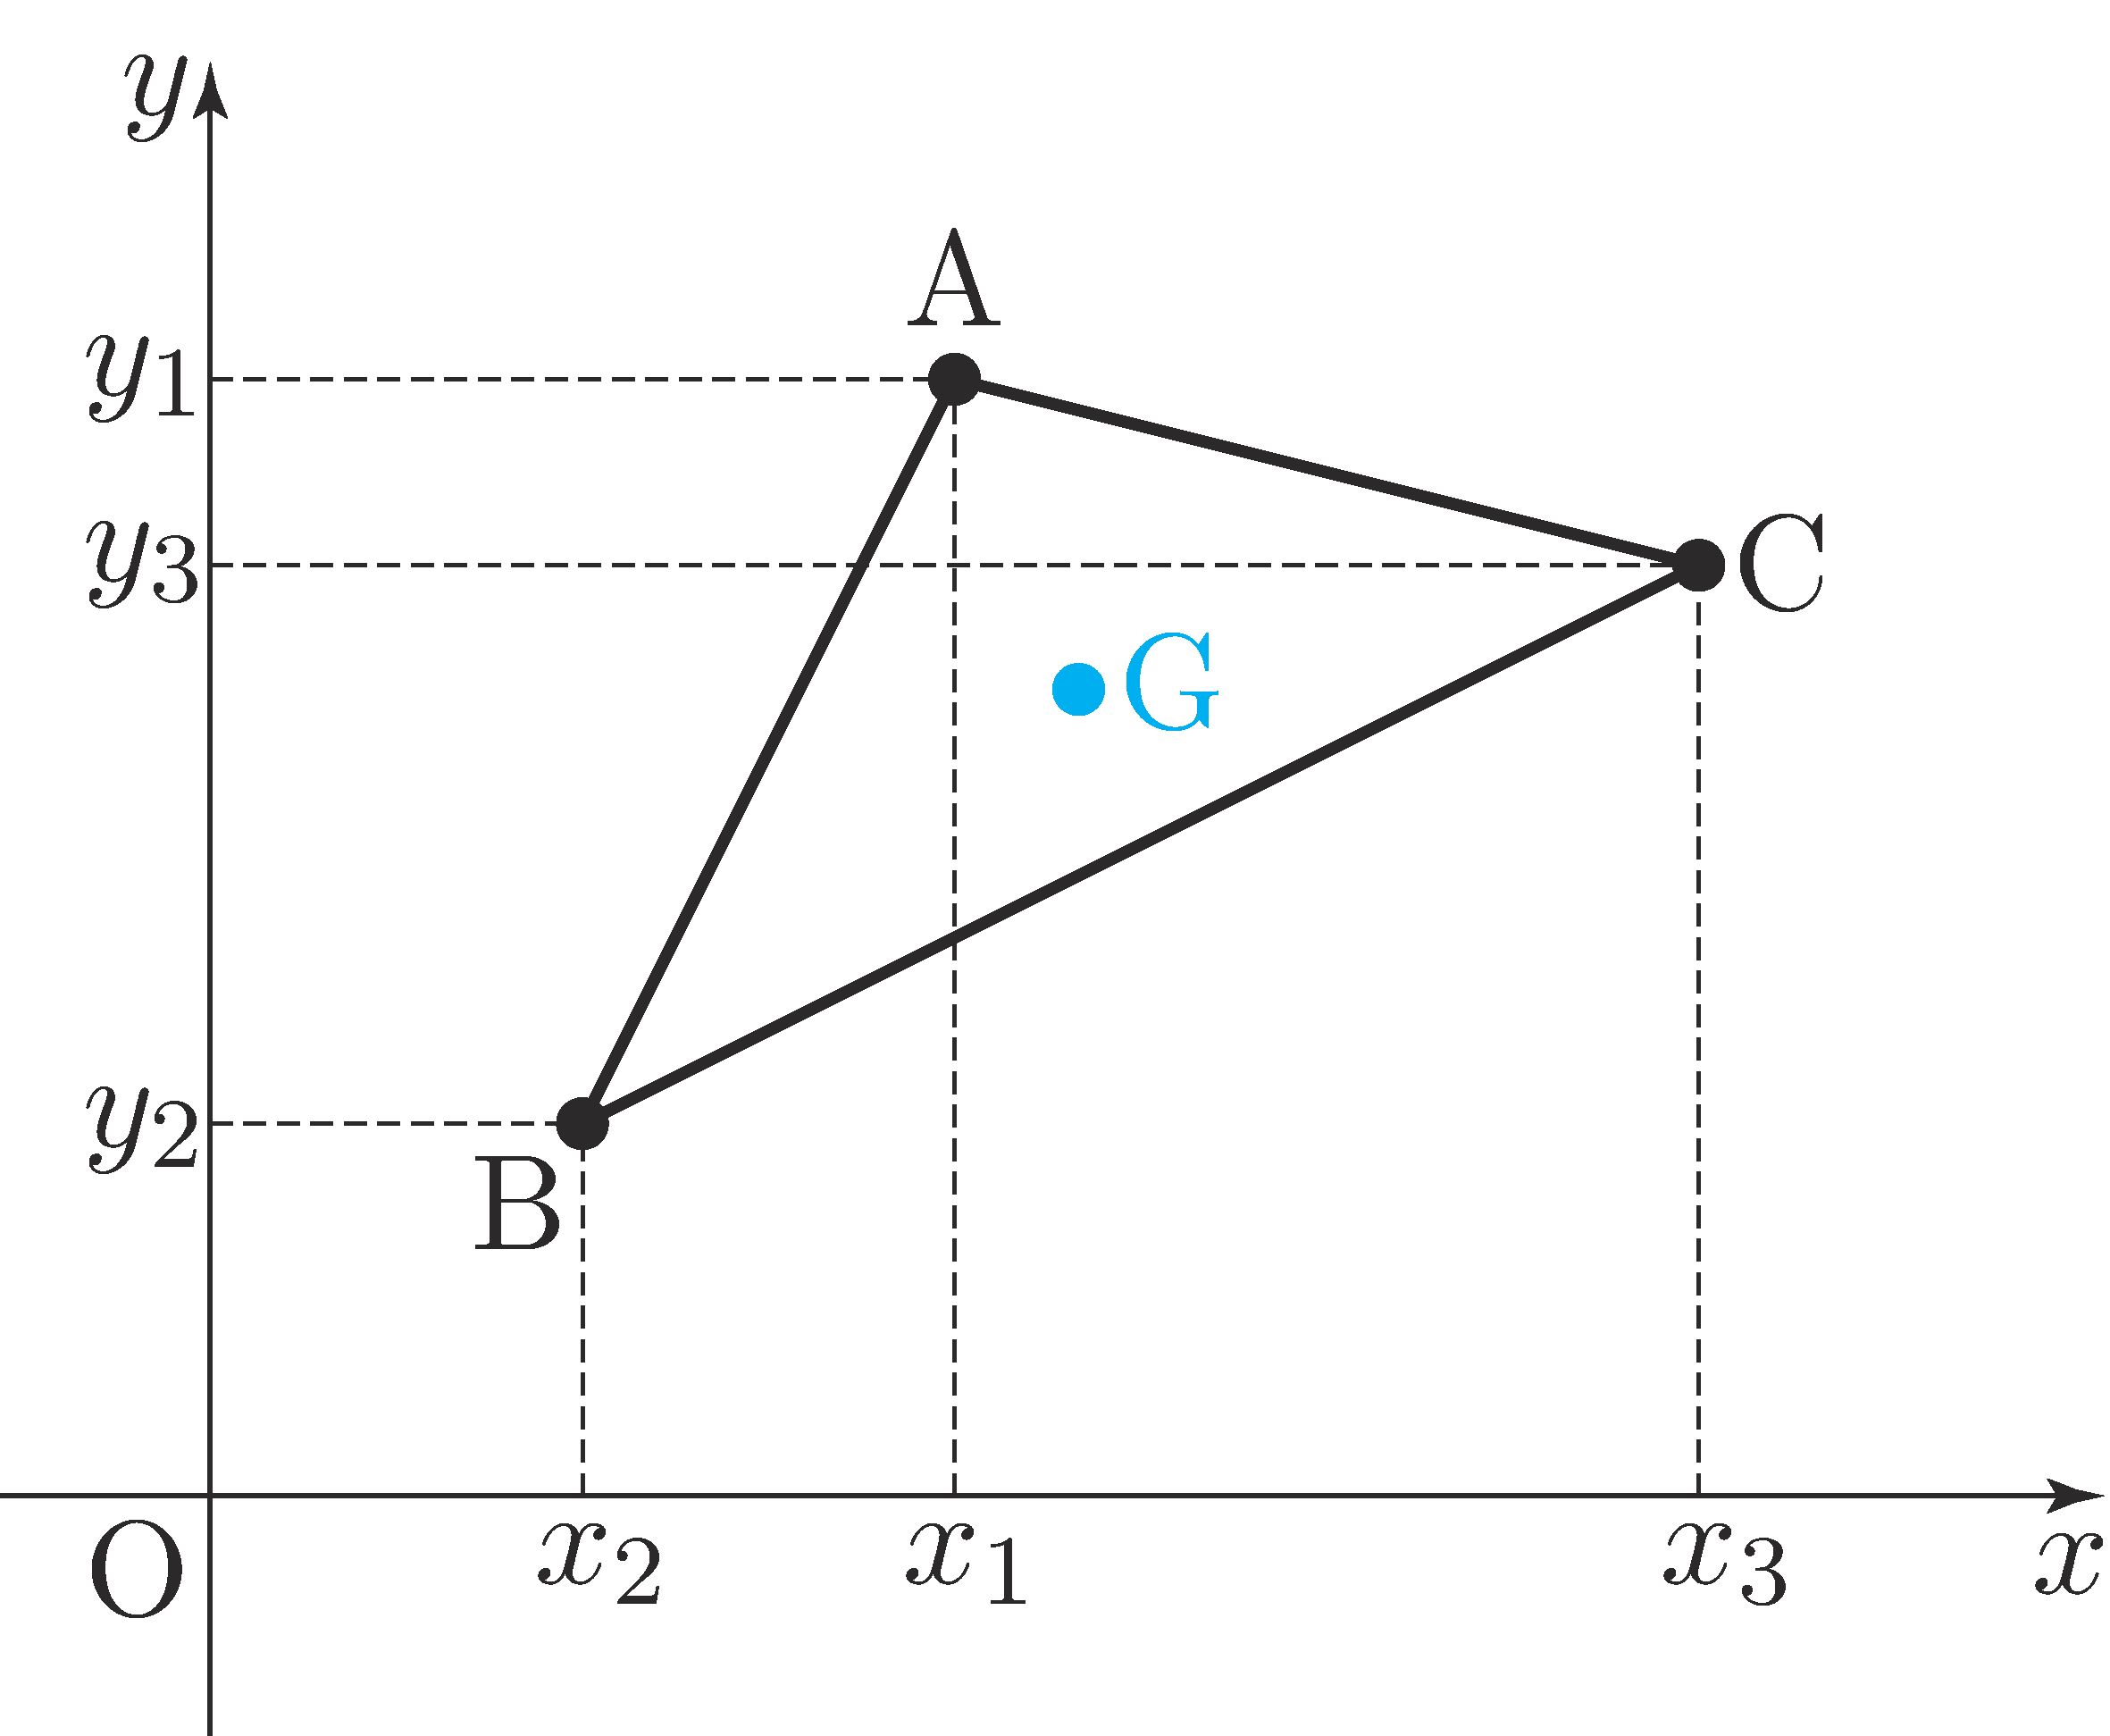
\includegraphics[scale=0.125]{pic0/pic146.pdf}\
\end{center}좌표평면에서 서로 다른 세 점 $\xy[A]{x_1}{y_1}$,  $\xy[B]{x_2}{y_2}$,  $\xy[C]{x_3}{y_3}$를 꼭짓점으로 하는 삼각형 $\mrm{ABC}$의 무게중심\mn[-5em]{삼각형의 무게중심은 각 꼭짓점과 마주보는 변의 중점을 이은 세 선분이 만나는 점입니다. 이때 각 선분이 무게중심에 의해 $1:2$로 내분된다는 특징이 있습니다.}{} $\mrm{G}$의 좌표는 다음과 같습니다. \begin{align*}\xy[G]{\dfrac{x_1 + x_2 + x_3}{3}}{\dfrac{y_1 + y_2 + y_3}{3}}\end{align*}
\clearpage
\section{도형의 방정식}
\subsection{직선의 방정식}\term[직선의 방정식]{좌표평면}{0}
\begin{center}
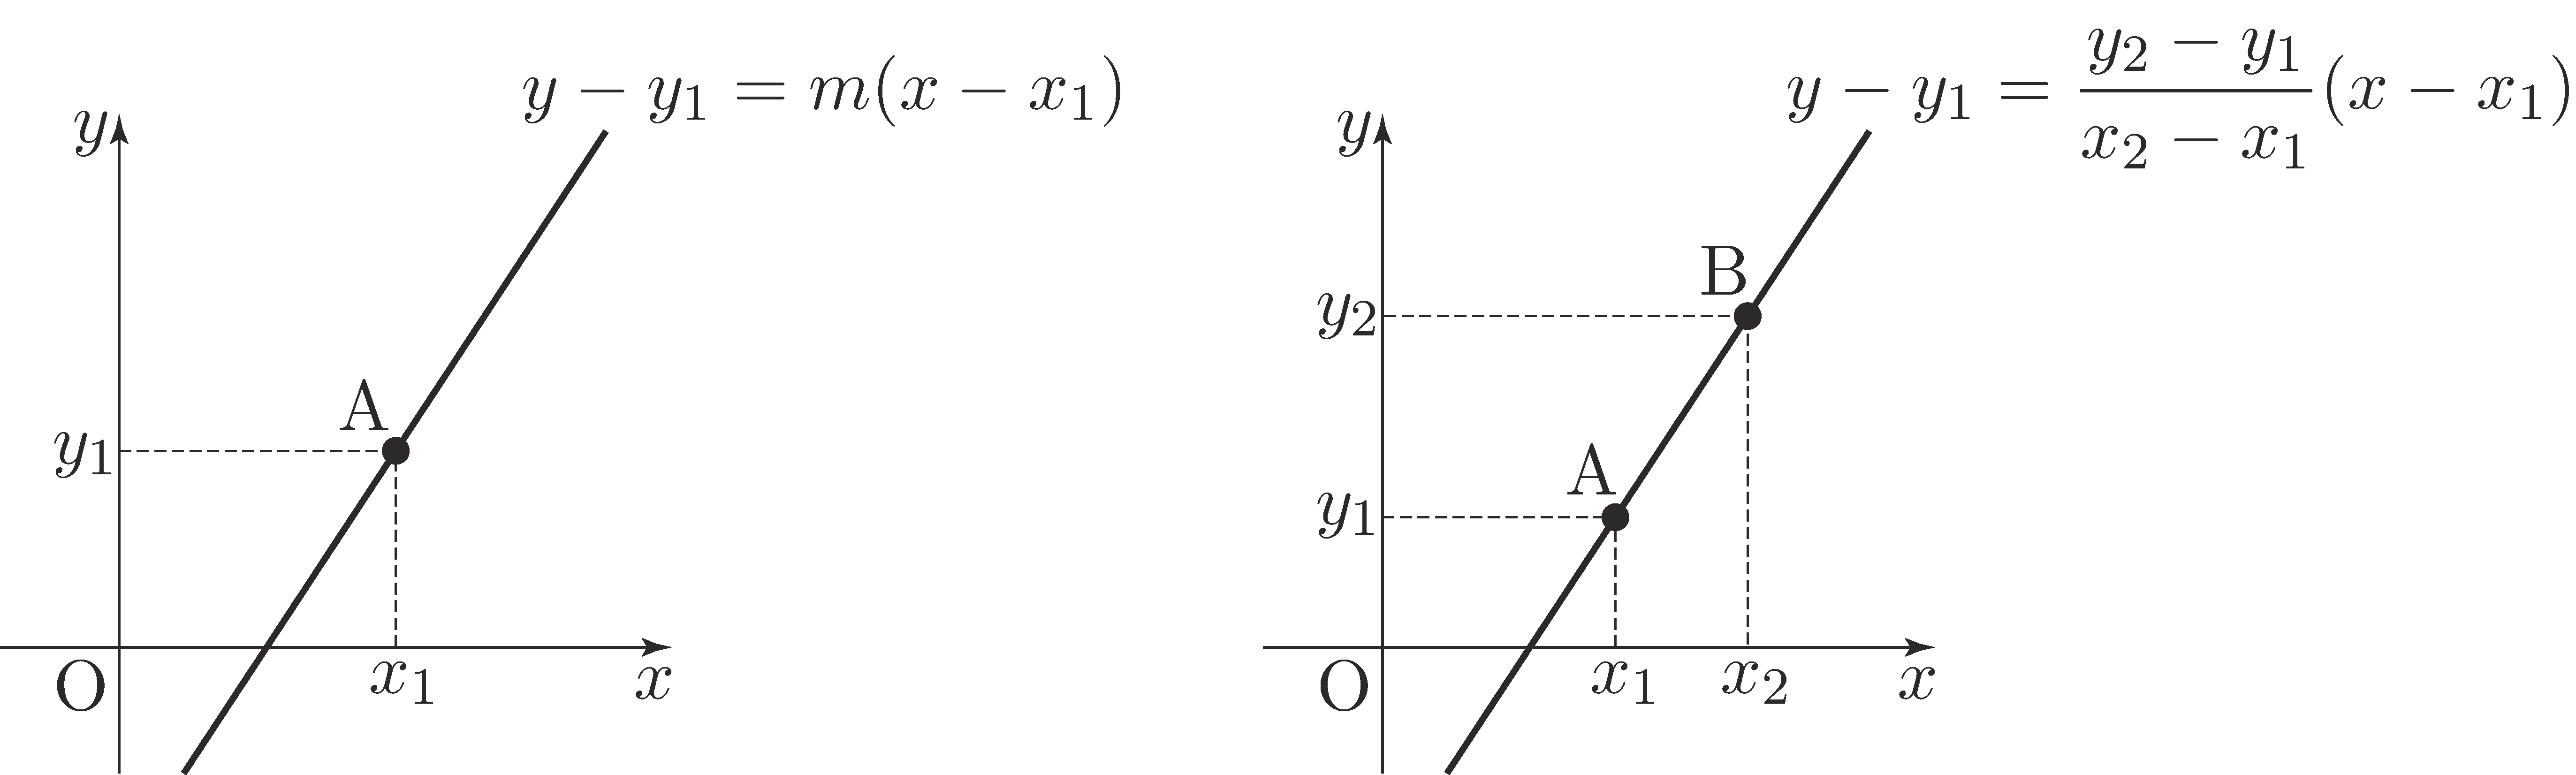
\includegraphics[scale=0.125]{pic0/pic147.pdf}
\end{center}좌표평면에서 한 점 $\xy[A]{x_1}{y_1}$을 지나고 기울기가 $m$인 직선의 방정식은 다음과 같습니다. \begin{align*}y-y_1 = m (x-x_1)\end{align*}
좌표평면에서 두 점 $\xy[A]{x_1}{y_1}$, $\xy[B]{x_2}{y_2}$를 지나는 직선의 방정식은 다음과 같습니다.
\begin{alignat*}{2}
  y-y_1 &= \dfrac{y_2-y_1}{x_2-x_1}(x-x_1) \quad &&(x_1 \ne x_2)\\
  x&=x_1 \quad &&(x_1 = x_2)
\end{alignat*}

한편 직선의 방정식의 일반적인 식은 일차방정식 $ax+by+c=0$의 꼴이며 이때 $a\ne0$ 또는 $b\ne0$입니다.
\subsubsection{두 직선의 평행과 수직}\term[평행!좌표평면에서]{두 직선의 평행조건}{0}\term[수직!좌표평면에서]{두 직선의 수직조건}{0}

\begin{figure}[h]
  \centering
  \subfloat[][]{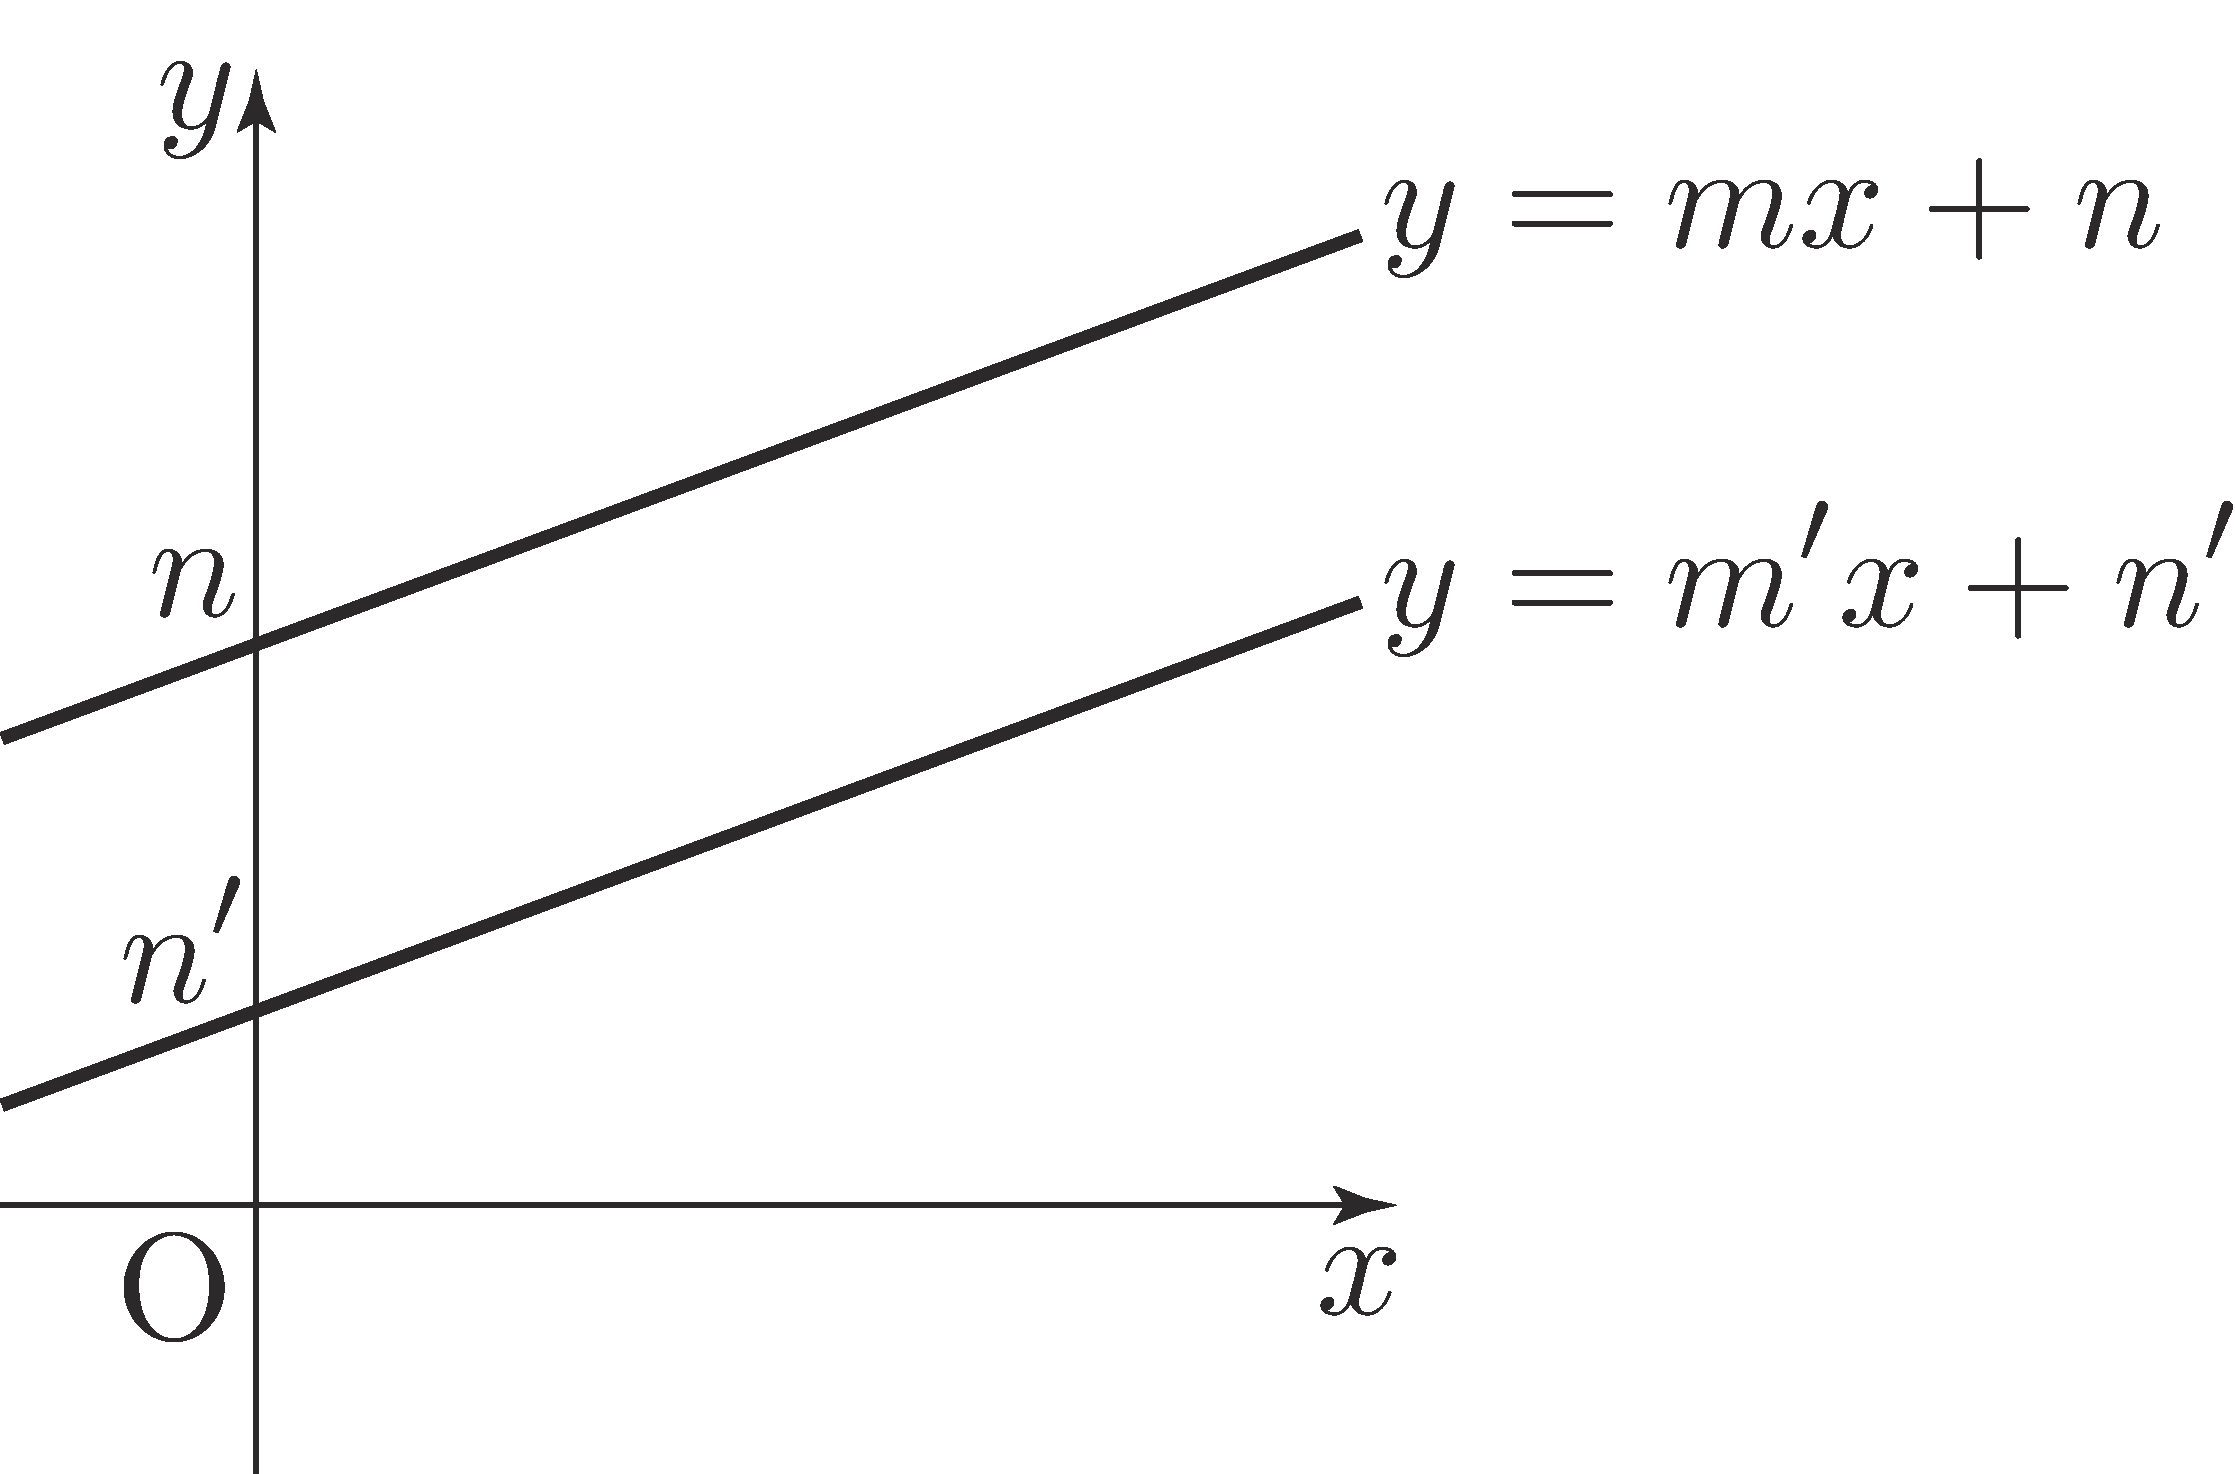
\includegraphics[scale=.125]{pic0/pic148_1.pdf}}
  \qquad
  \subfloat[][]{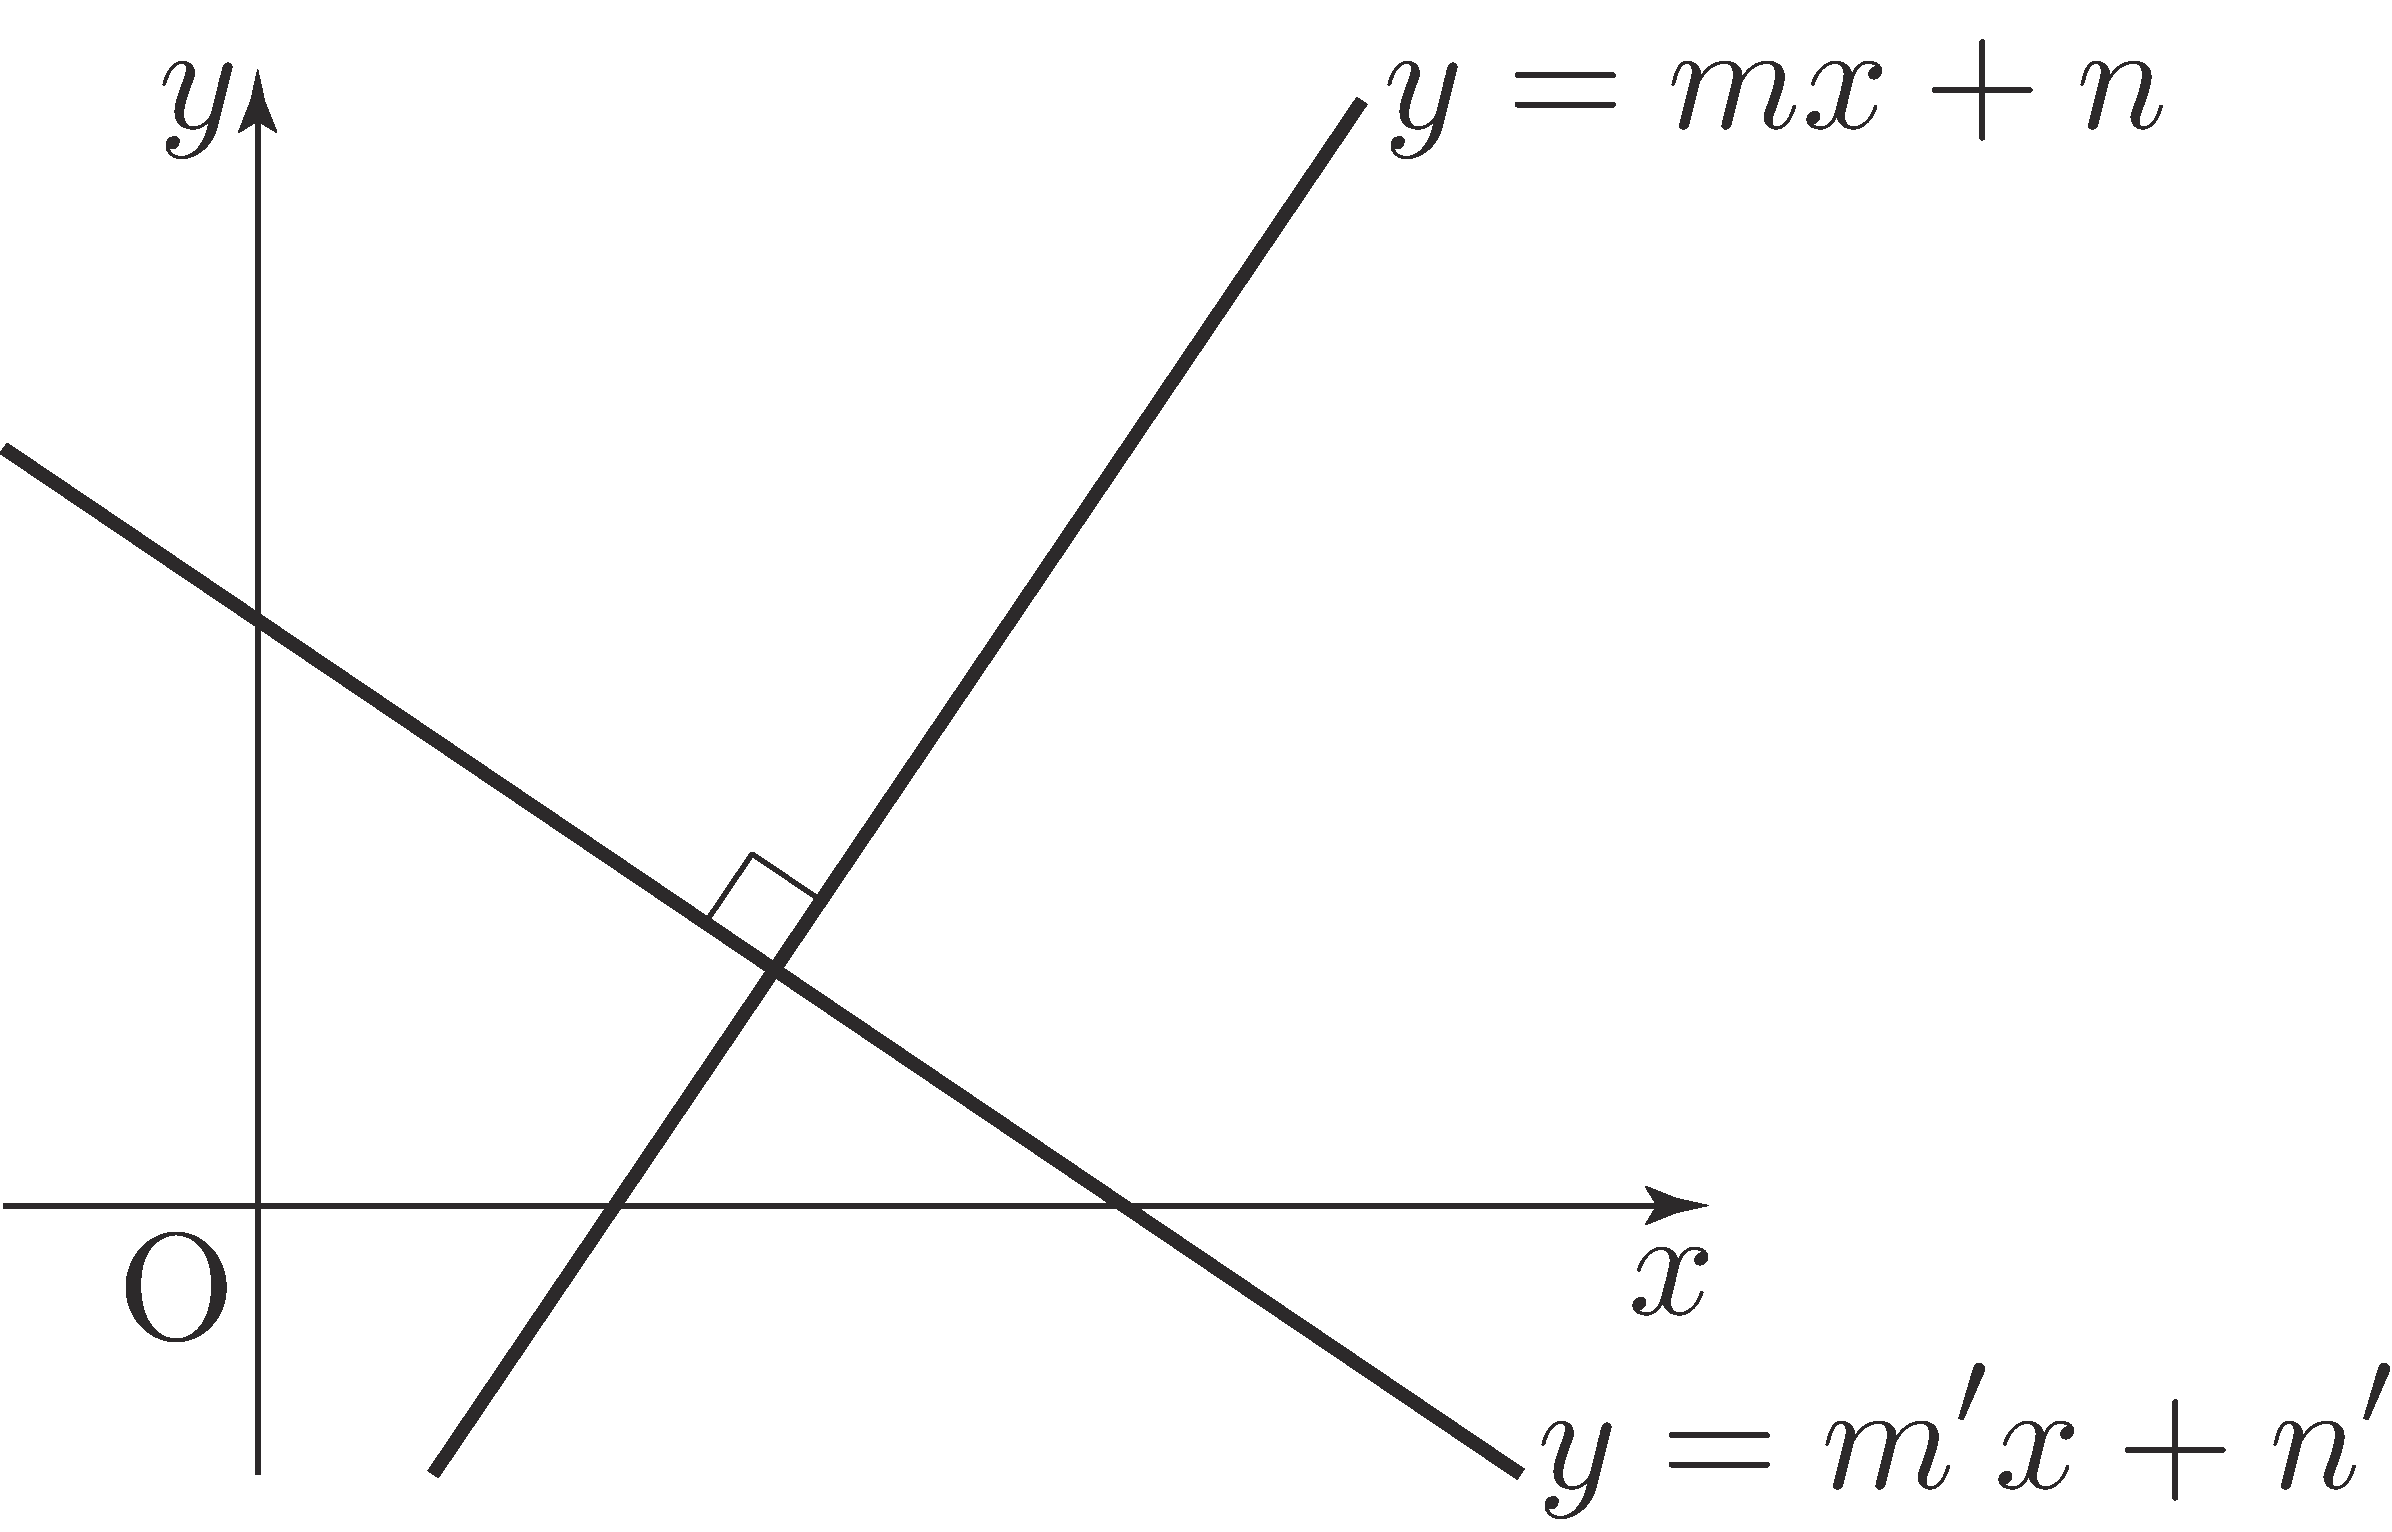
\includegraphics[scale=.125]{pic0/pic148_2.pdf}}
\end{figure}

(a)와 같이 두 직선 $y=mx+n$, $y=m'x+n'$이 서로 평행하면 $m=m'$, $n \ne n'$입니다. 반대로 $m=m'$, $n \ne n'$이면 두 직선이 평행합니다. (b)와 같이 $m \ne 0$, $m' \ne 0$이고 두 직선이 서로 수직이면 $mm' = -1$입니다. 반대로 $mm'=-1$이면 두 직선이 서로 수직입니다.

\subsubsection{점과 직선 사이의 거리}\term[거리!좌표평면]{점과 직선 사이의 거리}{0}
점 $\xy[P]{x_1}{y_1}$과 직선 $ax+by+c=0$ 사이의 거리 $d$는 다음과 같습니다.
\begin{align*} d = \dfrac{\abs{ax_1+by_1+c}}{\sqrt{a^2+b^2}} \end{align*}
\clearpage
\subsection{원의 방정식}\term[원!좌표평면]{원의 방정식}{0}
\begin{figure}[h]\centering \subfloat[][]{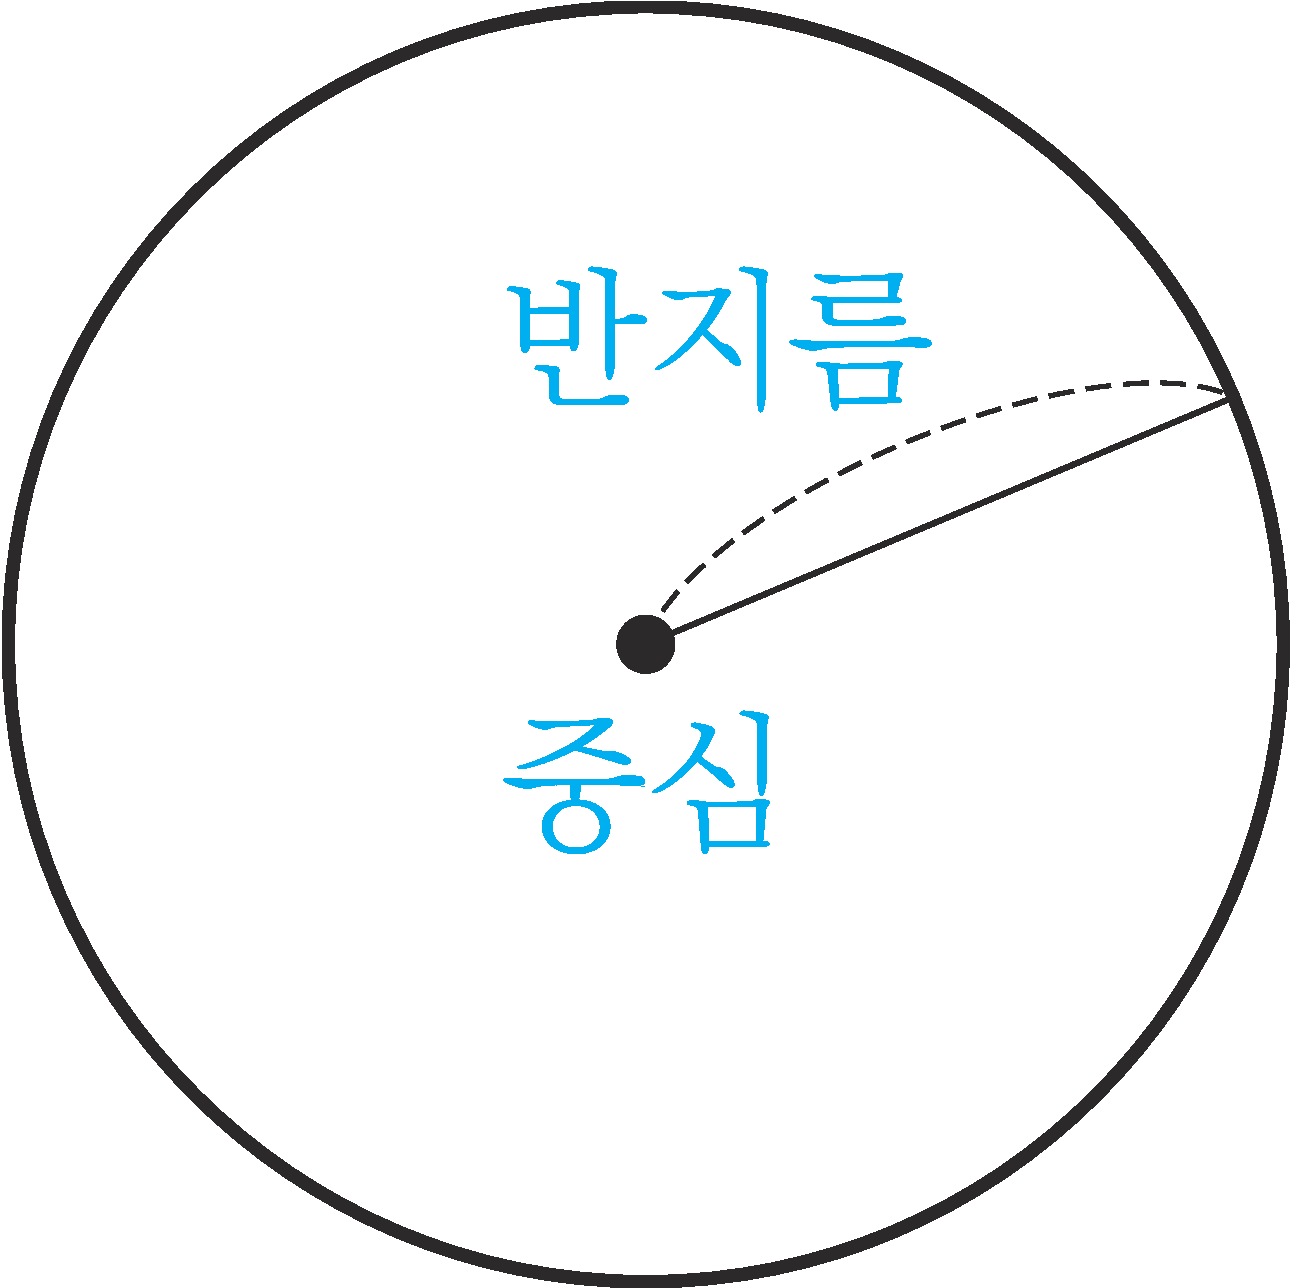
\includegraphics[scale=0.125]{pic0/pic162_1.pdf}}\
\qquad
\centering \subfloat[][]{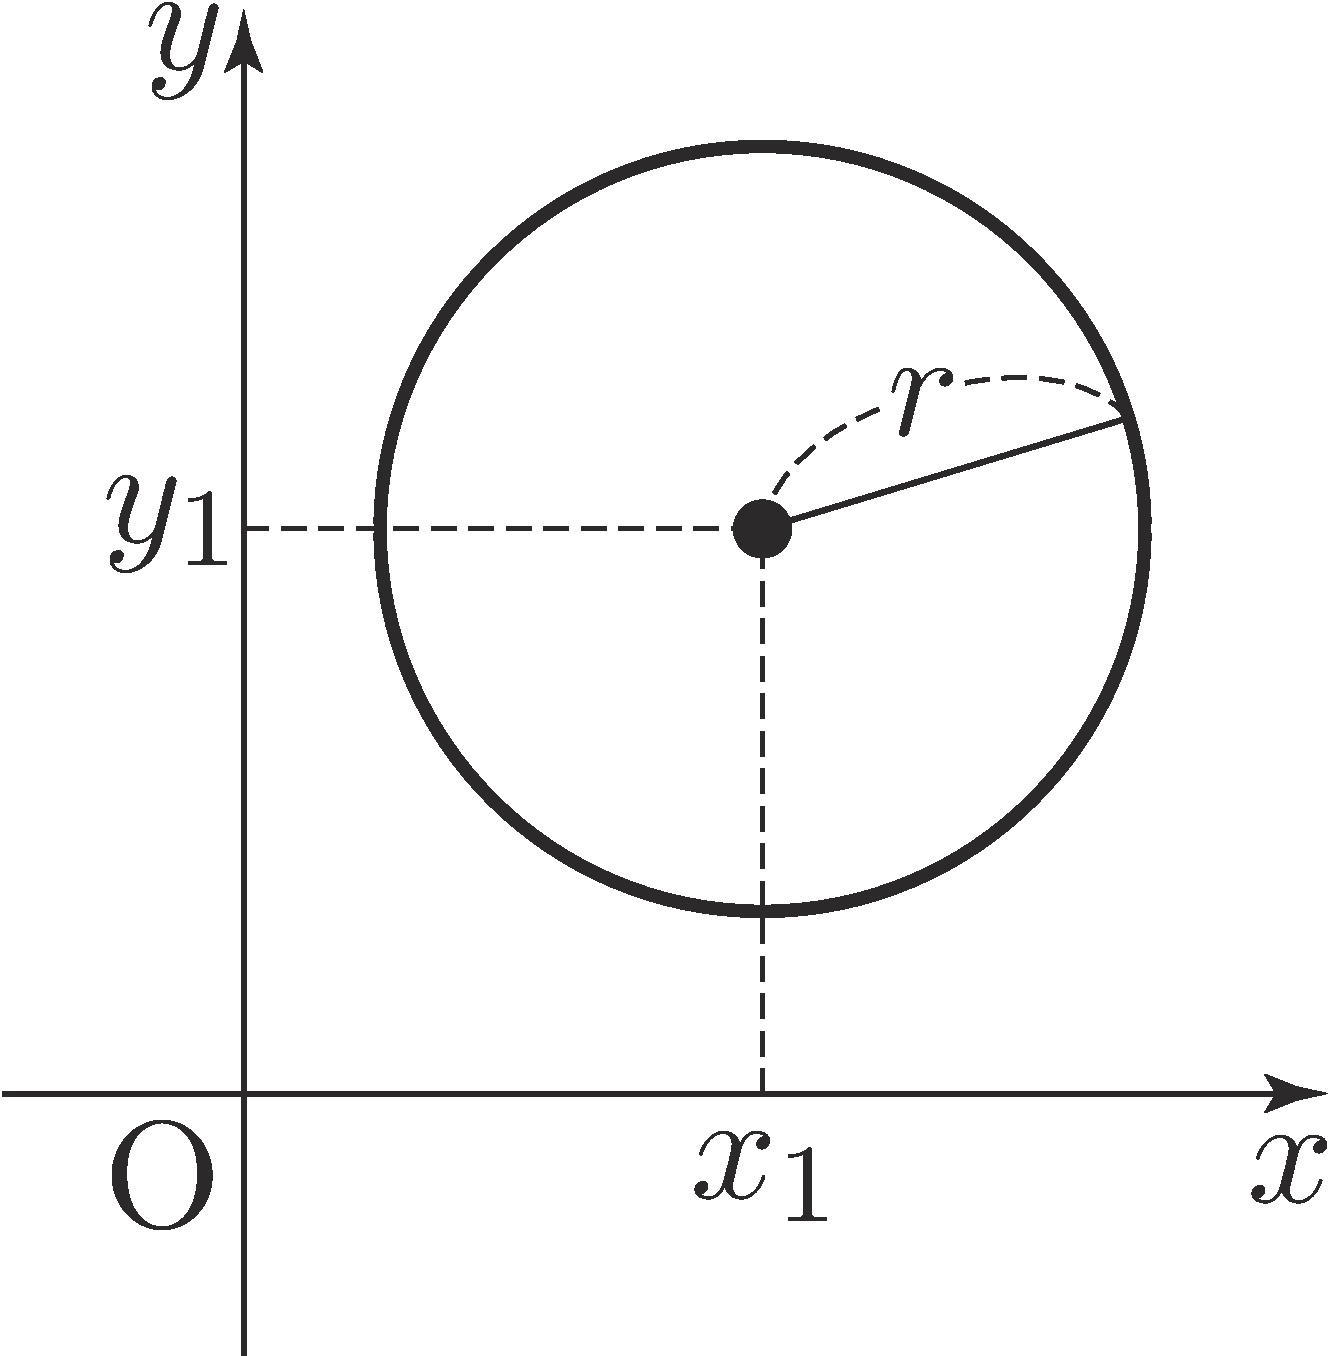
\includegraphics[scale=0.125]{pic0/pic162_2.pdf}}\
\end{figure}

(a)와 같이 평면에서 한 정점으로부터 일정한 거리에 있는 점 전체의 집합을 \term{원}{}이라고 합니다. 이때 정점을 원의 \term[원]{중심}{2}, 원의 중심과 원 위의 한 점을 이은 선분을 원의 \term[원]{반지름}{2}이라고 합니다. (b)와 같이 좌표평면에서 중심의 좌표가 $\xy[C]{x_1}{y_1}$이고 반지름의 길이가 $r$인 원의 방정식은 다음과 같습니다.
\begin{align*} (x-x_1)^2 + (y-y_1)^2 = r^2 \end{align*}

한편 원의 방정식의 일반적인 식은 이차방정식 $x^2 + y^2 + Ax + By + C = 0$의 꼴이며 이때 $A^2 + B^2 - 4C > 0$입니다.

\subsubsection{원과 직선의 위치관계}\term[원!좌표평면]{원과 직선의 위치관계}{0}
\begin{center}
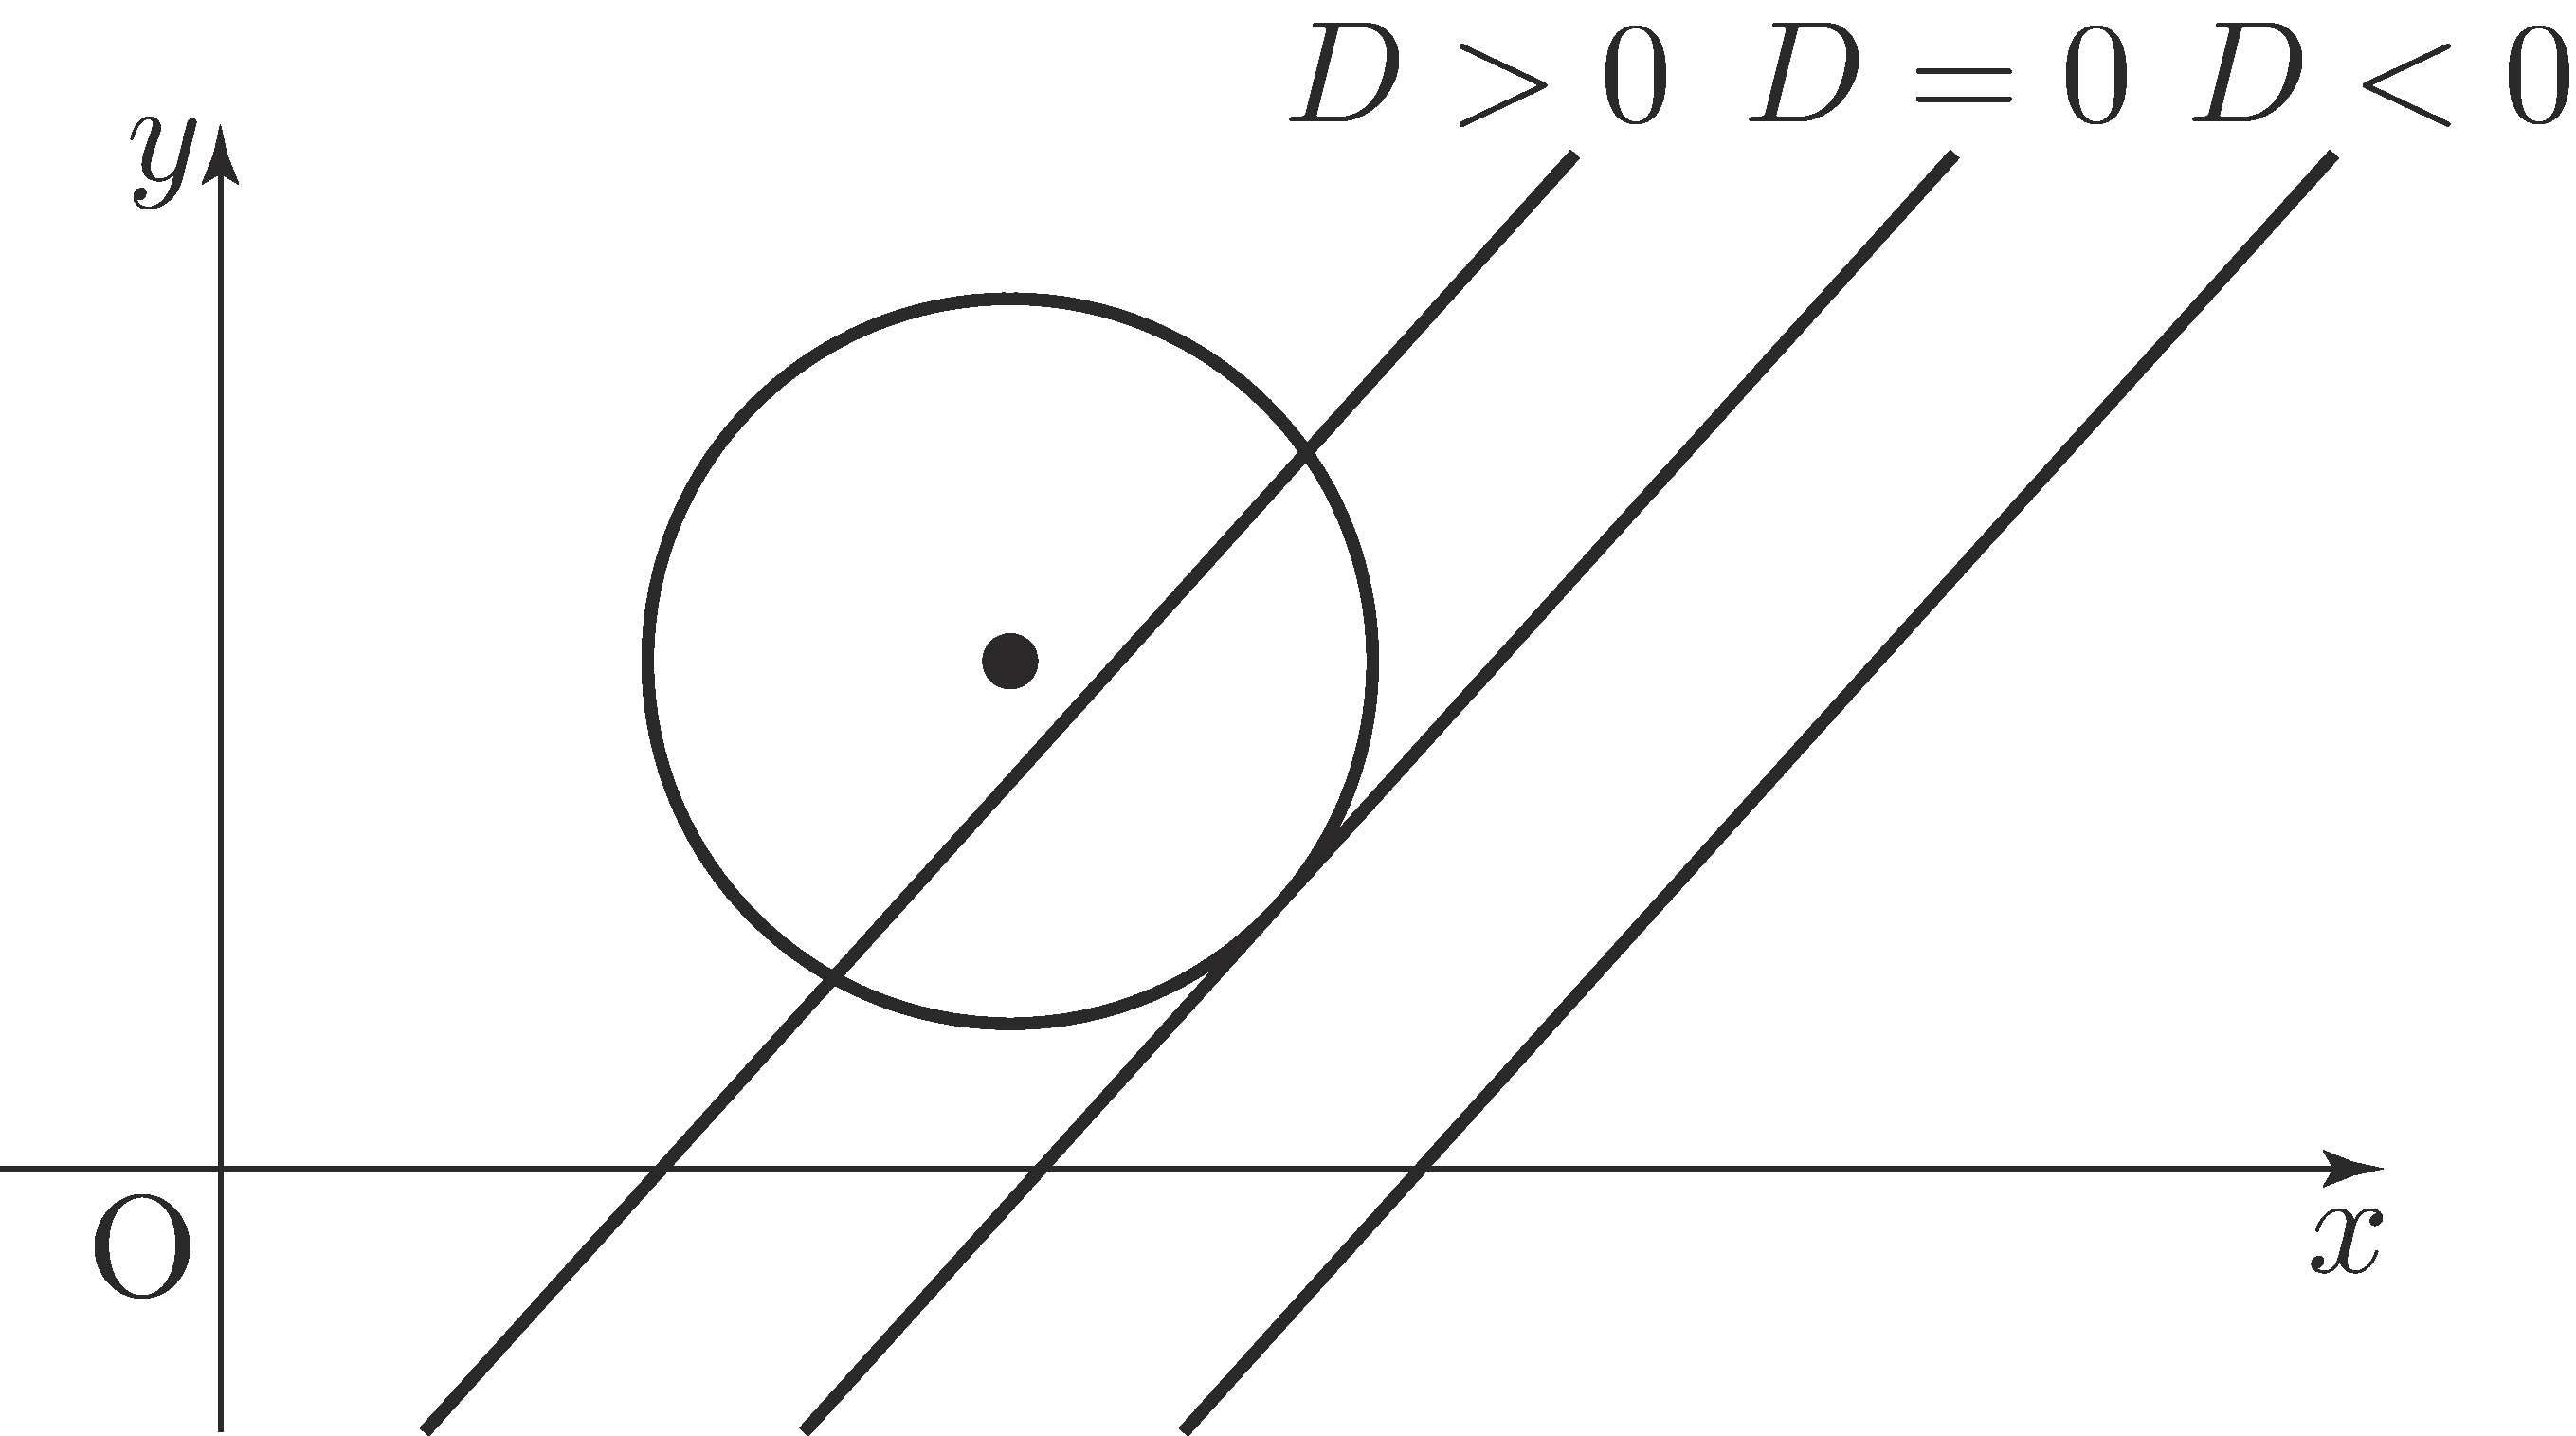
\includegraphics[scale=0.125]{pic0/pic163.pdf}\
\end{center}원 $x^2 + y^2 = r^2$과 직선 $y=mx+n$의 교점의 개수는 두 식을 연립한 이차방정식의 판별식 $D$의 부호에 따라 달라집니다. 반대로, 교점의 개수에 따라 $D$의 부호가 달라집니다.
\begin{justbox}
  \begin{enumerate}[label=\onum*]
    \item $D>0$ : 서로 다른 두 점에서 만난다.
    \item $D=0$ : 한 점에서 만난다. (접한다)
    \item $D<0$ : 만나지 않는다.
  \end{enumerate}
\end{justbox}
\clearpage
\section{평행이동과 대칭이동}

\subsection{평행이동}\term{평행이동}{0}
\begin{center}
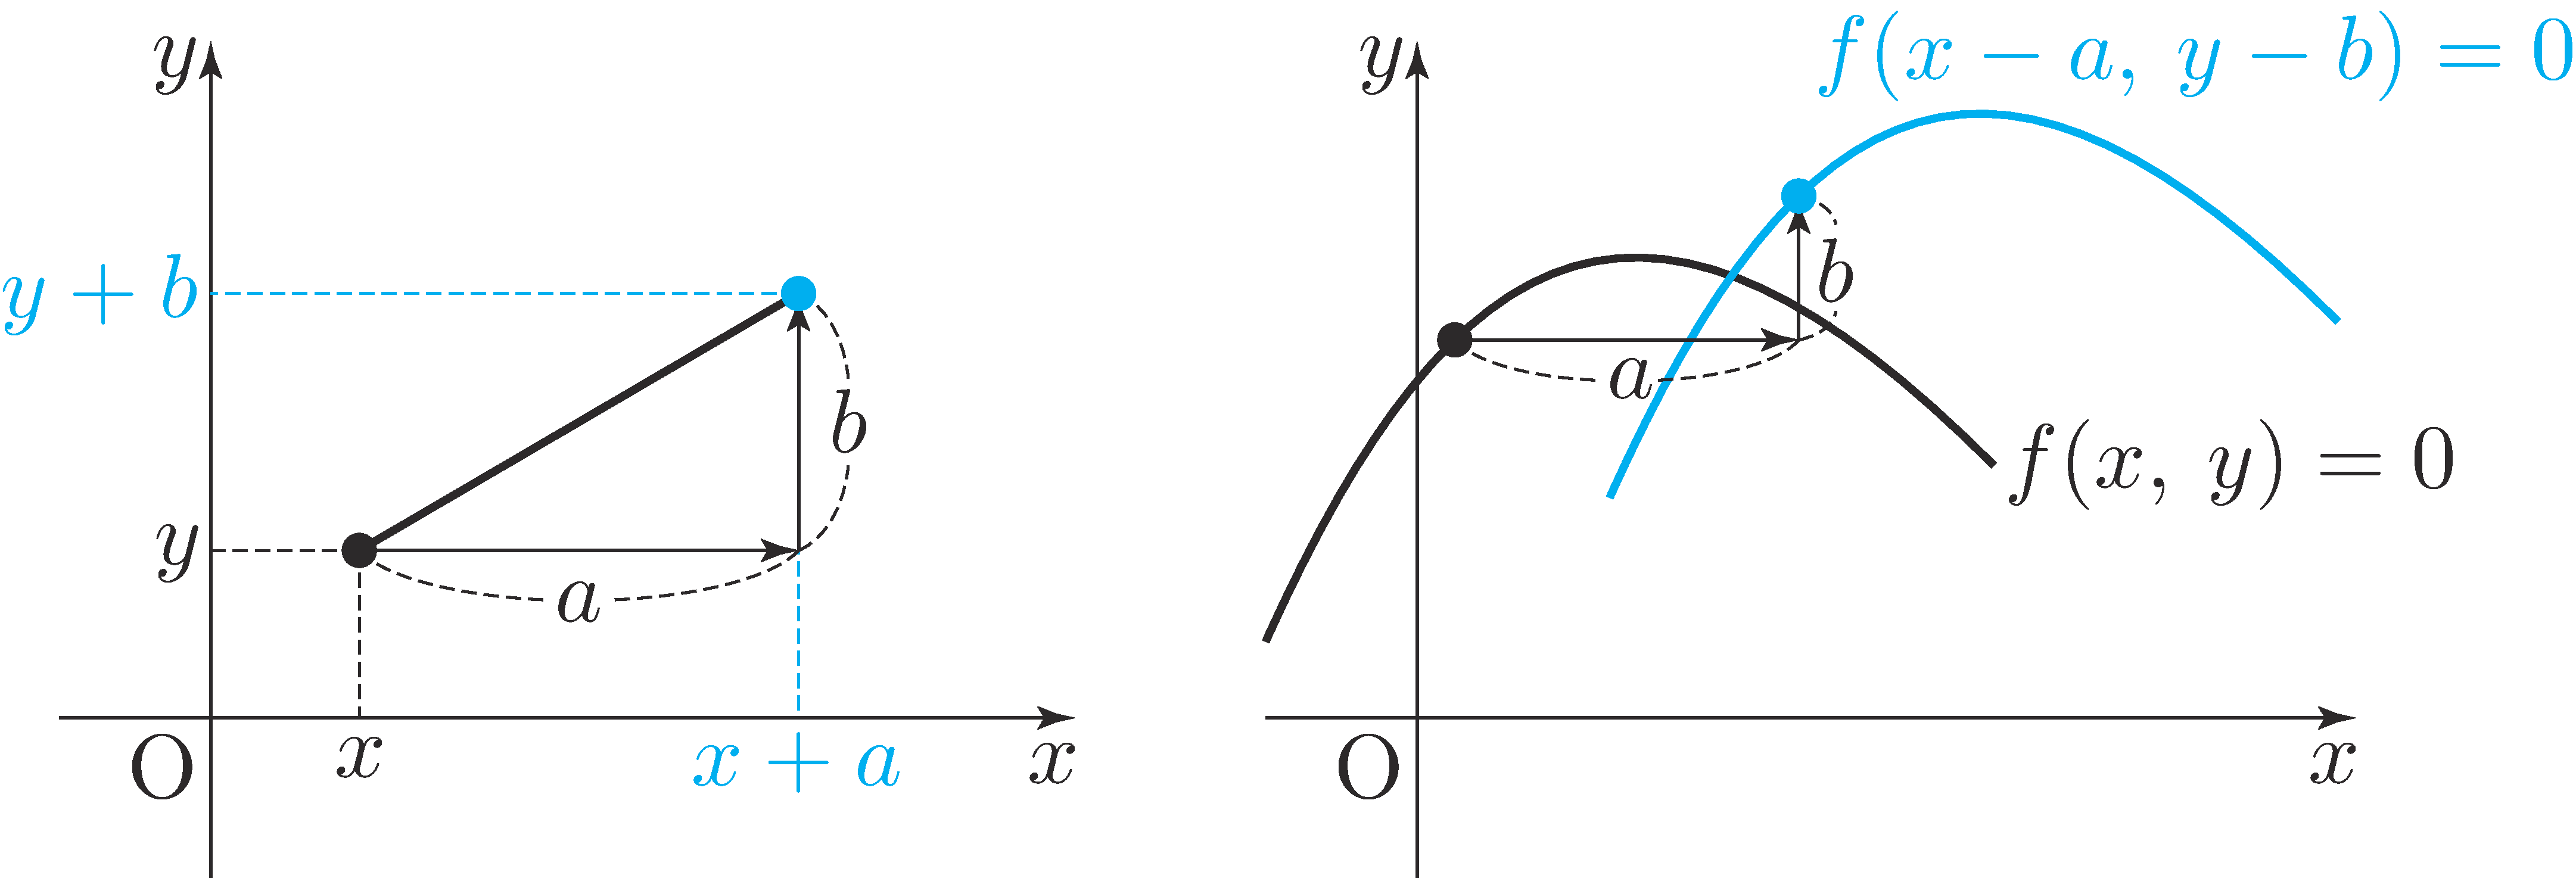
\includegraphics[scale=0.125]{pic0/pic149.pdf}
\end{center} 좌표가 $\xy{x}{y}$인 점을 $x$축 방향으로 $a$만큼, $y$축 방향으로 $b$만큼 평행이동한 점의 좌표는 $\xy{x+a}{y+b}$입니다. 도형 $f(x,\:y)=0$를 $x$축 방향으로 $a$만큼, $y$축 방향으로 $b$만큼 평행이동한 도형의 방정식은 $f(x-a,\:y-b)=0$입니다.

\subsection{대칭이동}\term{대칭이동}{0}
\begin{center}
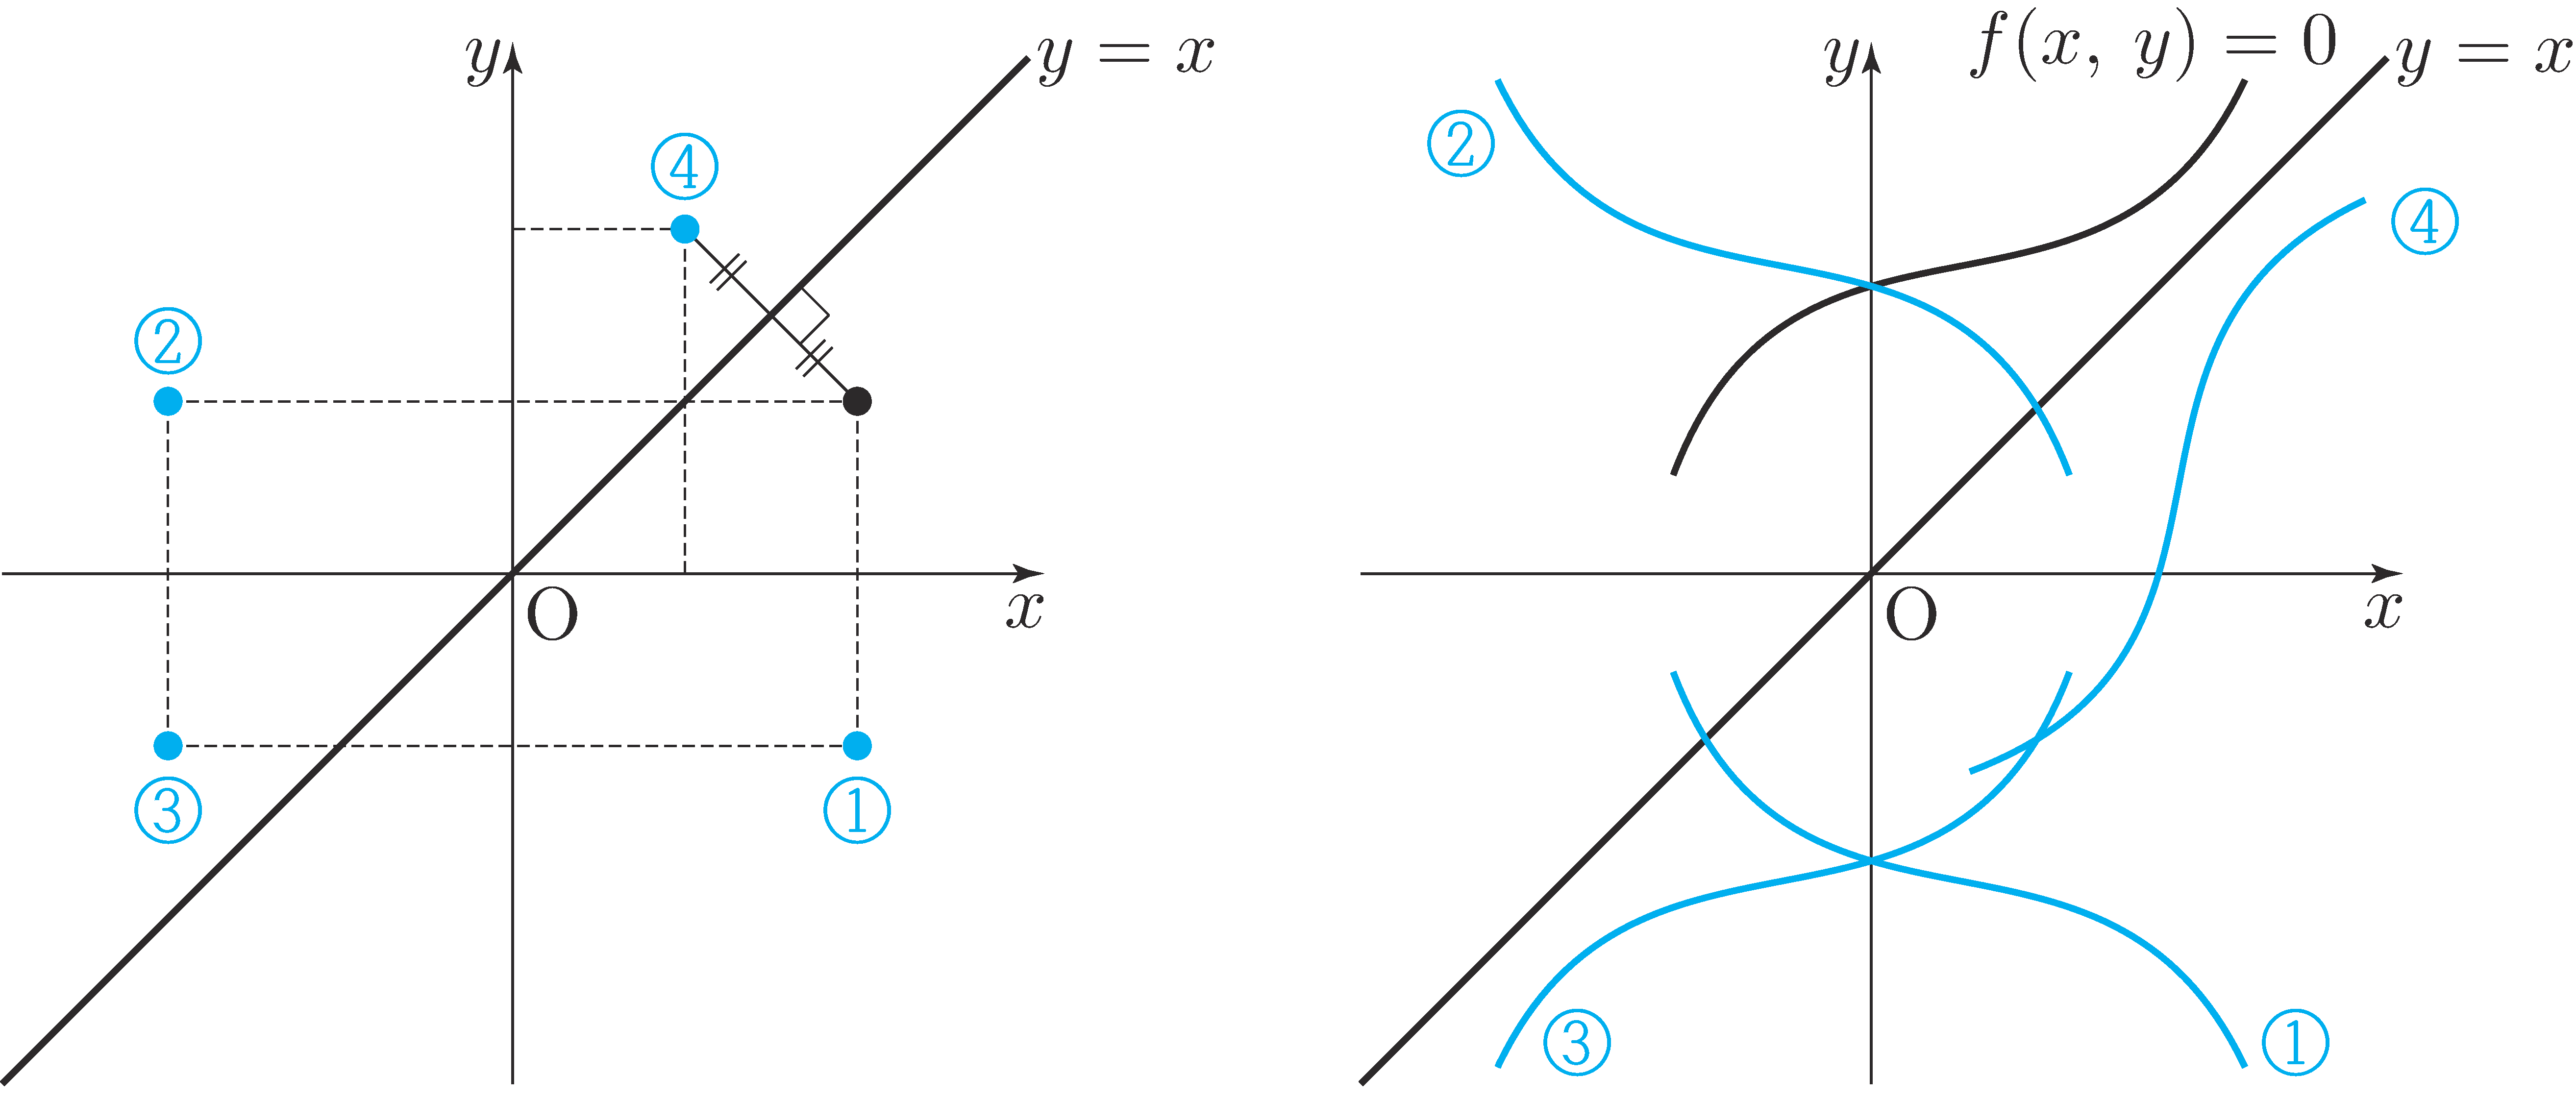
\includegraphics[scale=0.125]{pic0/pic150.pdf}
\end{center}좌표가 $\xy{x}{y}$인 점과 도형 $f(x,\:y)=0$을 $x$축, $y$축, 원점, 직선 $y=x$에 대하여 대칭이동한 점의 좌표와 도형의 방정식은 각각 다음과 같습니다.
\begin{justbox}
  \begin{enumerate}[label=\onum*]
    \item $x$축에 대하여 대칭이동 : $(x,\: -y)$, $f(x,\:-y)=0$
    \item $y$축에 대하여 대칭이동 : $(-x,\: y)$, $f(-x,\: y)=0$
    \item 원점에 대하여 대칭이동 :  $(-x,\: -y)$, $f(-x,\:-y)=0$
    \item 직선 $y=x$에 대하여 대칭이동 : $(y,\: x)$, $f(y,\: x)=0$
  \end{enumerate}
\end{justbox}


\cleartorecto\part{Zero 2) 함수와 연관된 기본 개념}\cleartoverso
\mychapter{함수}{}
\section{대응과 함수}  
\subsection{대응의 정의}
두 집합 $X$, $Y$에 대하여 집합 $X$의 원소에 집합 $Y$의 원소를 짝 지어 주는 것을 `$X$에서 $Y$로의 \term{대응}{}'이라고 합니다. 이때 집합 $X$의 원소 $x$에 집합 $Y$의 원소 $y$가 짝 지어지면 `$x$에 $y$가 \term{대응한다}{}'고 하며, 이것을 기호로 $x \longrightarrow y$와 같이 나타냅니다.

\subsection{함수의 정의}
두 집합 $X$, $Y$에 대하여 집합 $X$의 각 원소에 집합 $Y$의 원소가 오직 하나씩만 대응할 때, 이 대응을 `$X$에서 $Y$로의 \term{함수}{}'라고 합니다. 이를 기호로 나타내면 다음과 같습니다.\mn{함수의 이름은 관습적으로 $f$, $g$, $h$와 같이 짓습니다. 함수의 영문 이름이 function이기 때문입니다.}{}
\begin{align*} f : X \longrightarrow Y\end{align*}

\subsection{함수의 정의에 대한 추가설명}
함수의 정의는 문장의 길이가 짧음에도 불구하고 굉장히 깐깐한 제약조건을 담고 있습니다. 문장 성분별로 분석하여 대응이 함수가 되기 위한 제약조건을 알아보고, 제약조건으로 착각하기 쉽지만 제약조건이 아닌 것을 알아봅시다.

\begin{figure}[h]\centering \subfloat[][]{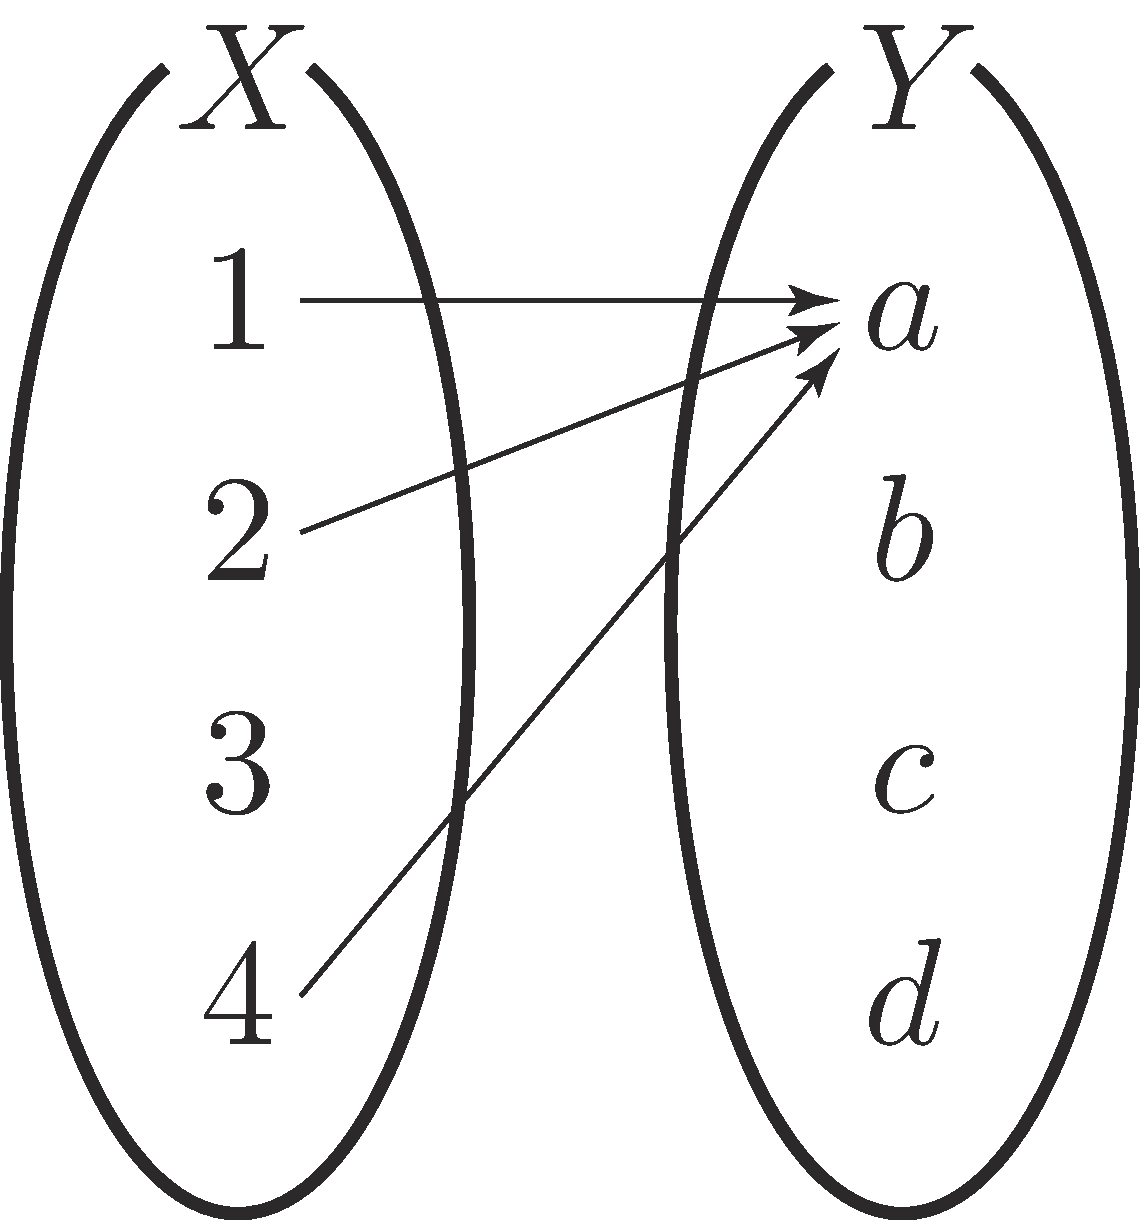
\includegraphics[scale=\pgfkeysvalueof{picsize}]{DBs/pic/zerg_01_1.pdf}}\
\qquad
\centering \subfloat[(2)][]{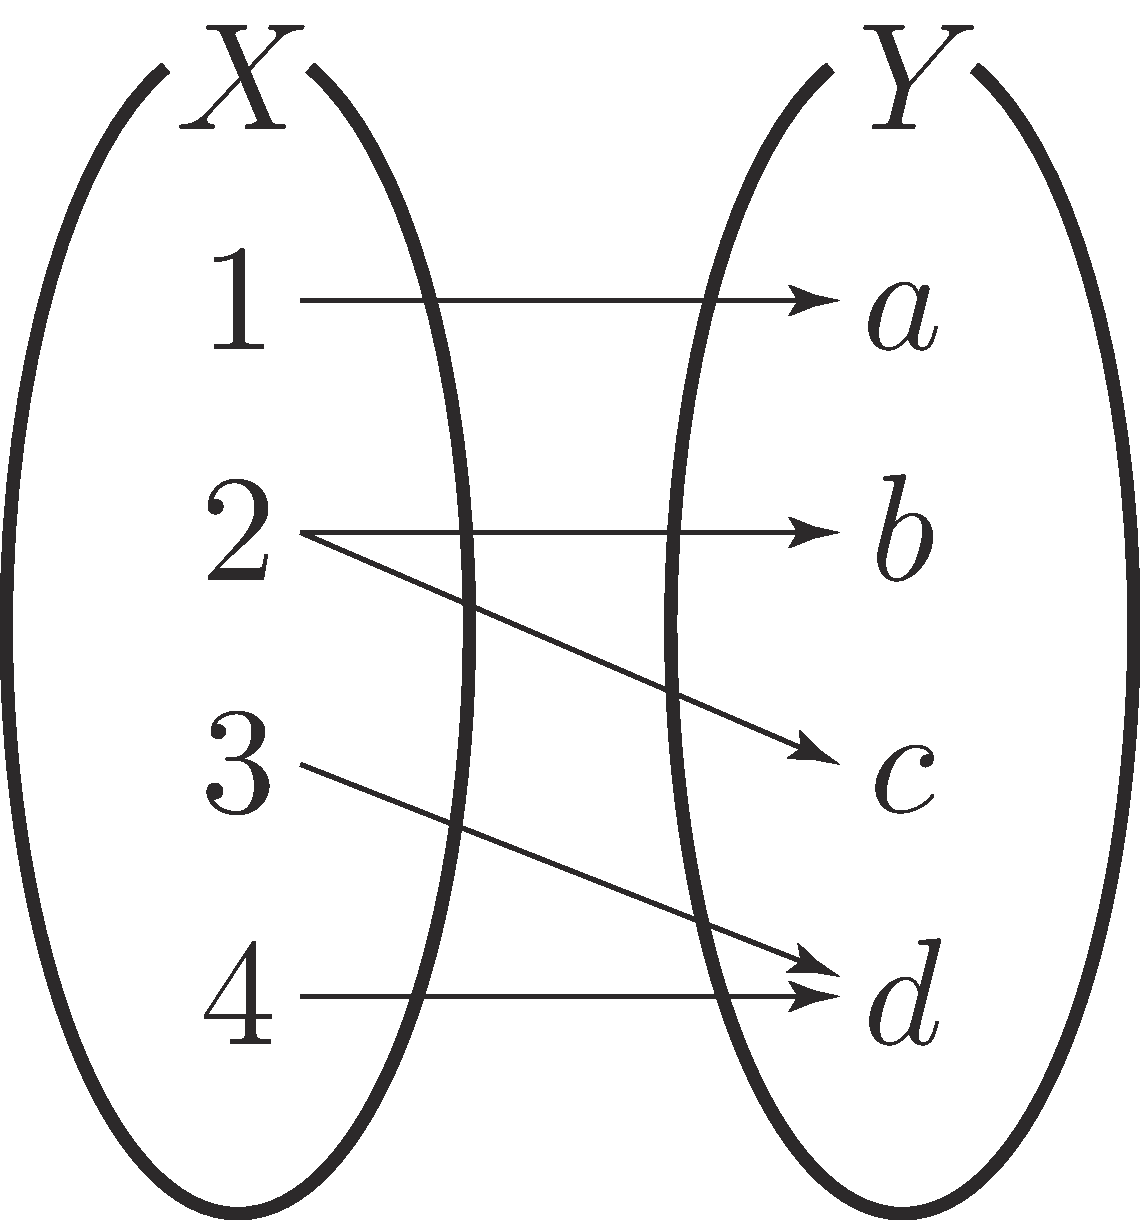
\includegraphics[scale=\pgfkeysvalueof{picsize}]{DBs/pic/zerg_01_2.pdf}}\
\qquad
\centering \subfloat[][]{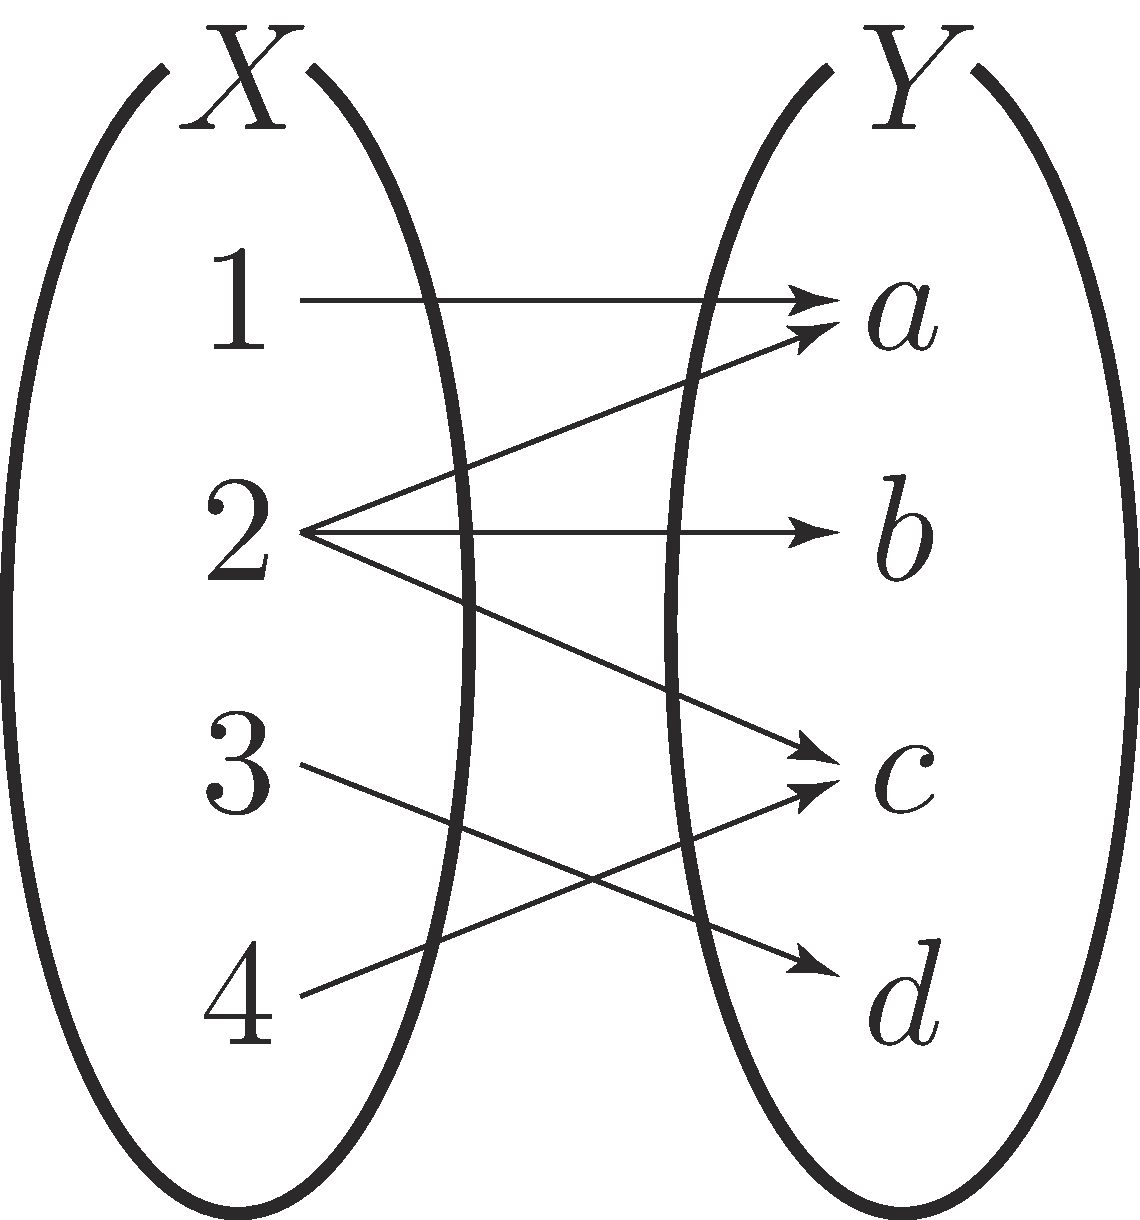
\includegraphics[scale=\pgfkeysvalueof{picsize}]{DBs/pic/zerg_01_3.pdf}}\
\qquad
\centering \subfloat[][]{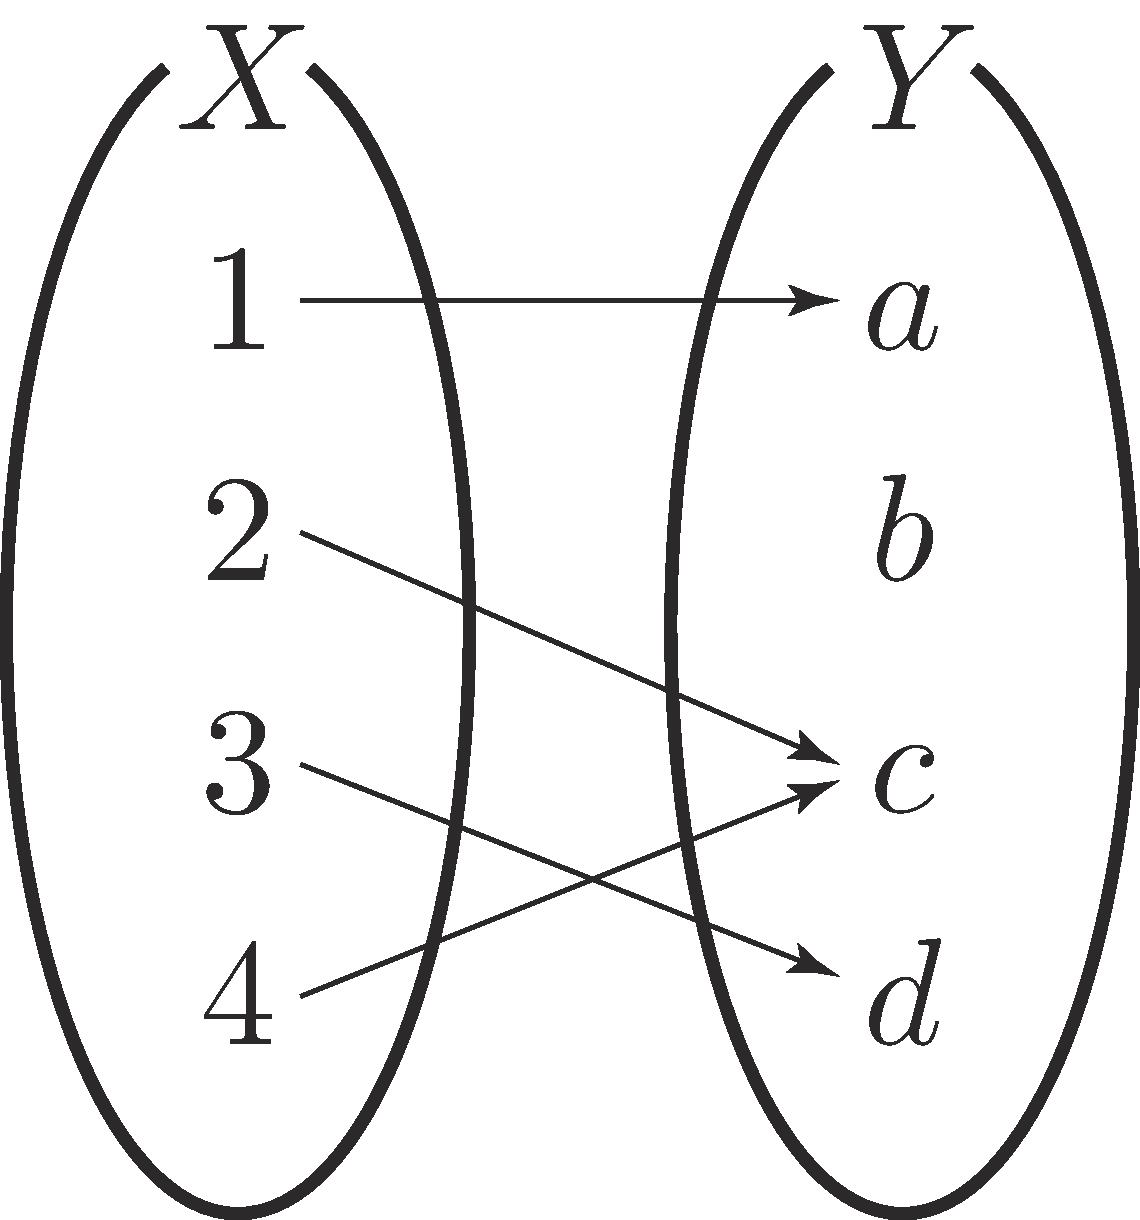
\includegraphics[scale=\pgfkeysvalueof{picsize}]{DBs/pic/zerg_01_4.pdf}}\
\end{figure}
\subsubsection{제약조건 (1) : 집합 $X$의 `각' 원소}
대응은 $X$의 원소 중 단 하나만 $Y$의 원소와 대응되더라도 관계없었습니다. 그러나 함수는 $X$의 각 원소가 하나도 빠짐없이 $Y$의 원소에 대응되어야 합니다. 

그림 (a)의 대응은 함수가 아닙니다. $X$의 원소인 $3$에 대응되는 $Y$의 원소가 없기 때문입니다.\mn{만약 집합 $Z=\left\{1,\: 2,\: 4\right\} $을 생각한다면 그림 (a)와 같은 상황에서 함수 $g:Z \longrightarrow Y$를 생각할 수는 있습니다.}{}  이와 달리 그림 (d)의 대응은 함수입니다.
\clearpage
\subsubsection{제약조건 (2) : 집합 $Y$의 원소가 `오직 하나씩만'}
대응은 $X$의 원소 하나에 $Y$의 원소 여러개가 대응되더라도 상관없었습니다. 함수는 $X$의 원소 하나에 대응되는 $Y$의 원소가 오직 하나여야(유일해야) 합니다. 

그림 (b), (c)의 대응은 함수가 아닙니다. `$X$의 원소인 $2$에 대응하는 $Y$의 원소'의 개수가 각각 $2$, $3$이기 때문입니다. 이와 달리 그림 (d)의 대응은 함수입니다.

\subsubsection{제약조건이 아닌 것 : $Y$의 모든 원소가 대응될 필요는 없다}
대응에서 $Y$의 모든 원소가 빠짐없이 대응될 필요는 없었듯이, 함수에서도 마찬가지입니다. 대응이 함수가 되기 위한 제약조건은 $X$의 원소, 그리고 $X$에 대응되는 $Y$의 원소에만 국한될 뿐임을 주의합시다.

\section{함수 관련 용어의 정의}
\subsection{정의역, 공역, 치역, 함숫값}
집합 $X$, $Y$와 함수 $f : X \longrightarrow Y$에 대하여 $X$를 함수 $f$의 \term{정의역}{}, $Y$를 함수 $f$의 \term{공역}{}이라 합니다. 또한 함수 $f$에 의하여 정의역의 원소 $x$에 공역의 원소 $y$가 대응할 때, 이를 등식으로 $y=f\left( x \right) $와 같이 나타내고, $f(x)$를 $x$에서의 \term{함숫값}{}이라고 합니다. 이때 함숫값 전체의 집합인 $\conset{f\left( x \right) }{$x\in X$}$를 함수 $f$의 \term{치역}{}이라고 합니다.

\subsection{`제약조건'과 정의역, 함숫값}
제약조건 (1)에 따르면, 정의역에 포함된 임의의 원소 $x$에 대하여 함숫값 $f(x)$가 항상 존재합니다. 제약조건 (2)에 따르면, 정의역에 포함된 임의의 원소 $x$에 대하여 $f(x)$의 값은 유일합니다.\mn{이 문장에서 말하는 것은 `$x$의 값에 관계 없이 $f(x)$의 값이 같다'는 것이 아니라, $f(3)=3$인 동시에 $f(3)=5$일 수 없다는 것입니다. `$x$의 값에 관계 없이 $f(x)$의 값이 같은 함수'에 대해서는 곧 뒤에서 배웁니다.}{} 


\subsection{`제약조건이 아닌 것'과 치역, 공역}
어떤 함수의 공역을 $Y$, 치역을 $F$라 할 때, `제약조건이 아닌 것'에 따르면, 치역과 공역이 항상 일치하는 것은 아닙니다. 한편, 치역은 $Y$의 원소 중에서 함숫값 $f(x)$가 될 수 있는 원소들로 이루어진 집합이므로, 치역은 공역의 부분집합입니다. 따라서 $F$가 $Y$의 진부분집합이면 공역과 치역이 일치하지 않습니다.

\subsection{정의역과 공역의 범위}
함수 $y=f\left( x \right) $의 정의역과 공역이 주어진 경우에는 정의역과 공역의 범위를 주어진 대로 취합니다. 함수 $y=f\left( x \right) $의 정의역과 공역이 주어지지 않는 경우에는 특별한 이유가 없는 한 $f(x)$가 정의되는 실수 $x$의 값 전체의 집합을 정의역으로, 실수 전체의 집합을 공역으로 생각합니다.\mn{특별한 이유의 대표적인 예시는 `일대일함수를 일대일대응이 되도록 공역을 치역에 맞추어 축소시키기'가 있습니다.}{}
\clearpage
\section{함수의 서로 같음}
두 함수 $f$, $g$가 다음을 만족시킬 때, `두 함수 $f$, $g$는 \term{서로 같다}{}'고 하고, $f=g$와 같이 나타냅니다.
\begin{justbox}
    \begin{enumerate}[label={\onum*}]
            \item 정의역과 공역이 각각 서로 같다.
            \item 정의역의 모든 원소 $x$에 대하여 $f(x)=g(x)$이다.
        \end{enumerate}
\end{justbox}
예를 들어 $f\left( x \right) =\dfrac{x^2-1}{x-1}$과 $g\left( x \right) =x+1$는 $x\ne1$인 모든 실수 $x$에 대하여 $f\left( x \right)=g\left( x \right)$가 성립하므로 두 함수 $f$, $g$가 서로 같다고 착각하기 쉽습니다. 그러나 정의역이 같을 수 없으므로\mn[-3\blskip]{단, $f$와 $g$의 정의역에서 $x = 1$을 제외해주면 정의역을 같게 해줄 수 있습니다.}{} 두 함수 $f$, $g$는 서로 같지 않습니다.

\section{함수의 그래프} 
함수 $f:X \longrightarrow Y$에서 정의역 $X$의 원소 $x$와 이에 대응하는 함숫값 $f(x)$의 순서쌍 $\xy{x}{f(x)}$ 전체의 집합 $G=\conset{\xy{x}{f\left( x \right) }}{$x \in X$}$를 함수 $f$의 \term{그래프}{}라고 합니다.\mn[-2\blskip]{그래프를 그림 그 자체라고 생각하는 경우가 많지만, 정의에 따르면 그래프는 집합이지 그림이 아닙니다. 그림은 그 집합을 좌표평면에 나타내었을 때 드러나는 형상일 뿐입니다.}{}  정의역과 치역이 각각 $\mathbb{R}$의 부분집합인 함수 $y=f(x)$의 그래프는 순서쌍 $\xy{x}{f\left( x \right) }$를 좌표평면에 점으로 나타내어 그릴 수 있습니다.
\clearpage
\section{여러 가지 함수}
\subsection{일대일함수와 일대일대응}
다음 조건을 만족시키는 함수 $f: X \longrightarrow Y$를 \term{일대일함수}{}라 합니다.
\begin{justbox}
    정의역 $X$의 임의의 두 원소 $x_1$, $x_2$에 대하여 $x_1 \ne x_2$이면 $f\left( x_1 \right) \ne f\left( x_2 \right) $이다.
\end{justbox}
다음 조건을 만족시키는 함수 $f: X \longrightarrow Y$를 \term{일대일대응}{}이라 합니다.\mn{교과서에서는 `일대일 대응'으로 띄어쓰고 있지만, 그 띄어쓰기의 기준이 일관되지 않습니다. 따라서 불필요한 혼동을 피하기 위하여 붙여쓰도록 하겠습니다.}{}
\begin{justbox}
    \begin{enumerate}[label=\onum*]
        \item $f$가 일대일함수이다.
        \item $f$의 공역과 치역이 서로 같다. 
    \end{enumerate}
\end{justbox}

\begin{center} 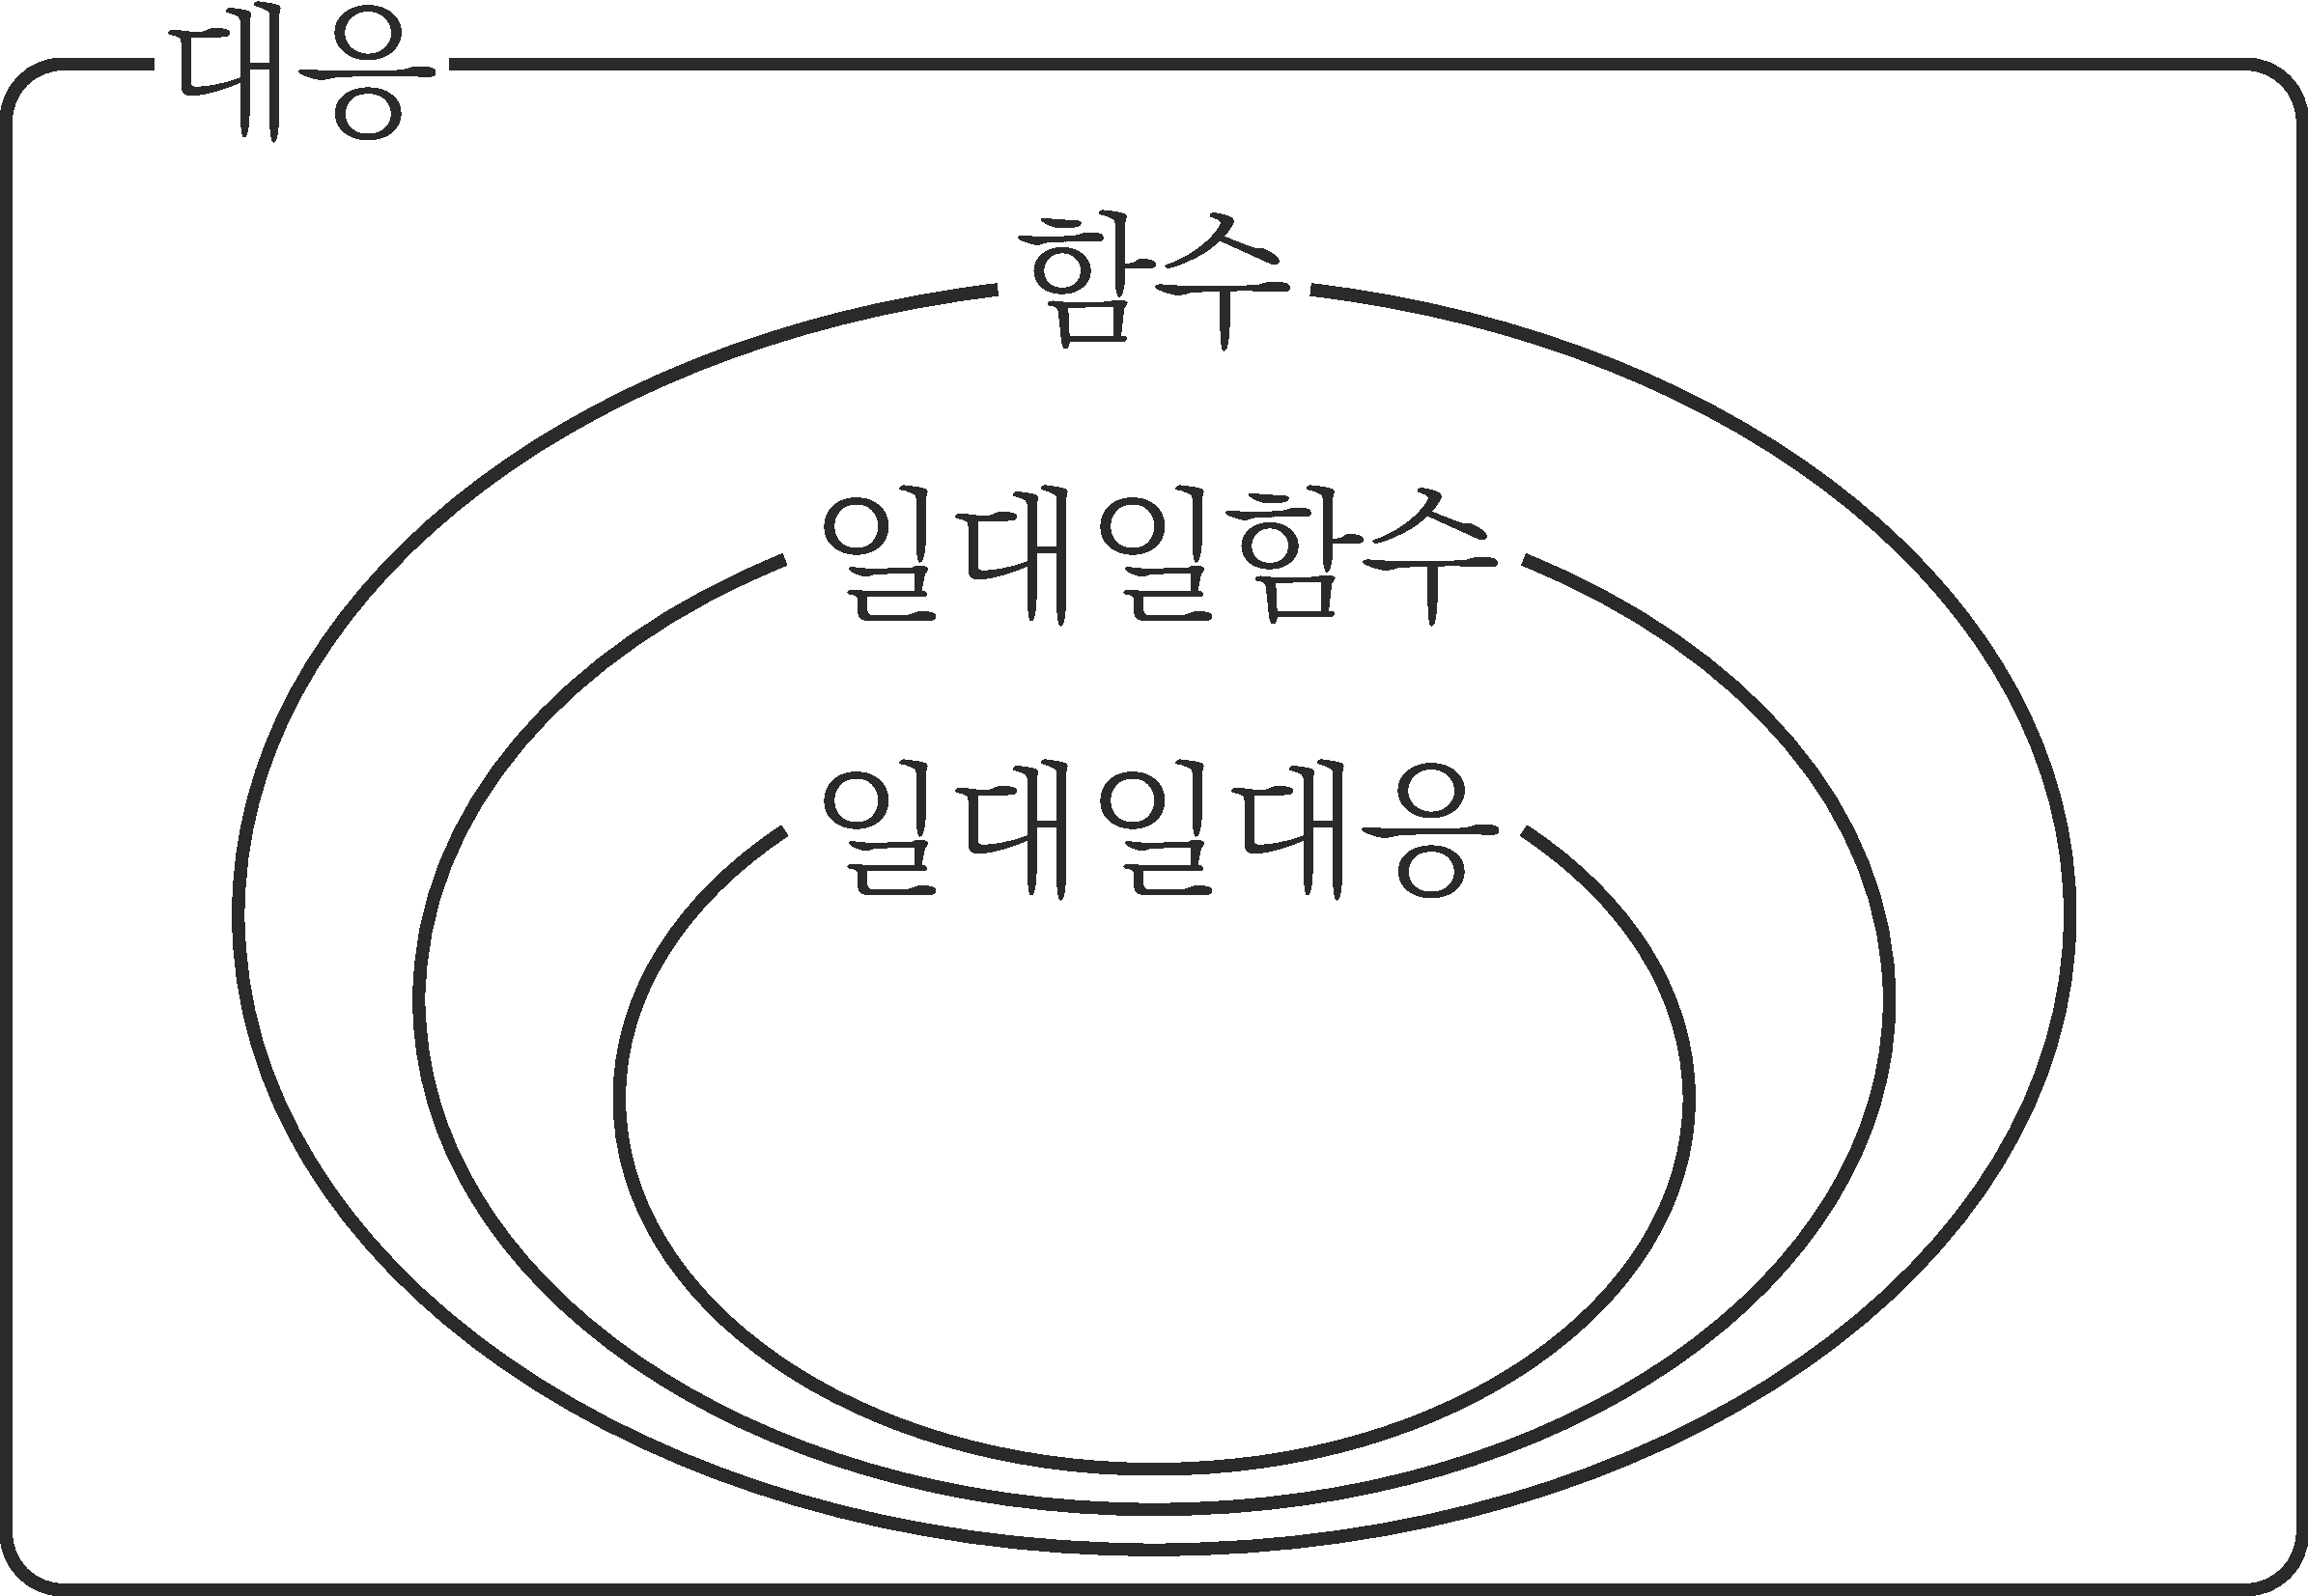
\includegraphics[scale=\pgfkeysvalueof{picsize}]{DBs/pic/zerg_02.pdf}\\
	\end{center}일대일함수, 일대일대응, 함수, 대응의 관계를 벤 다이어그램으로 나타내면 위 그림과 같습니다. 함수 $f$가 일대일대응이면 일대일함수입니다. 함수 $f$가 일대일함수이면 일대일대응일 수도 있고, 일대일대응이 아닐 수도 있습니다. 함수 $f$가 일대일함수가 아니라면 일대일대응도 아닙니다. 

\subsection{항등함수와 상수함수}
함수 $f:X \longrightarrow X$에서 정의역 $X$의 각 원소에 자기 자신이 대응할 때, 즉 $f\left( x \right) = x$일 때, 함수 $f$를 `$X$에서의 \term{항등함수}{}'라고 합니다.

함수 $f:X \longrightarrow Y$에서 정의역 $X$의 각 원소에 각각 모두 공역 $Y$의 원소 $c$가 대응할 때, 즉 $f\left( x \right) = c\:\left( \text{단, $c$는 상수} \right) $일 때, 함수 $f$를 \term{상수함수}{}라고 합니다.
\clearpage
\section{함수의 합성}
\subsection{합성함수의 정의}
일반적으로 두 함수 $f:X \longrightarrow Y$, $g:Y \longrightarrow Z$가 주어졌을 때, 집합 $X$의 임의의 원소 $x$에 대하여 함숫값 $f\left( x \right) $는 집합 $Y$의 원소이고, 집합 $Y$의 원소 $f\left( x \right) $에 대하여 함숫값 $g\left( f\left( x \right)  \right) $는 집합 $Z$의 원소입니다. 

이때 집합 $X$의 각 원소 $x$에 집합 $Z$의 원소 $g\left( f\left( x \right)  \right) $를 대응시키면, 이 대응은 $X$에서 $Z$로의 새로운 함수입니다. 이 함수를 `$f$와 $g$의 \term{합성함수}{}'라고 하며, 이것을 기호로 나타내면 다음과 같습니다.
\begin{align*} g \circ f, \quad  g \circ f : X \longrightarrow Z, \quad  y=g\left( f\left( x \right)  \right)  \end{align*}

\subsection{합성함수의 성질}
함수의 합성에서 교환법칙은 성립하지 않고, 결합법칙은 성립합니다. 따라서 여러 합성을 연달아 해야 할 때에는 아무렇게나 해서는 안 되고, 어떤 연산을 먼저 해야 결과가 최대한 간단해질 지를 따지는 것이 필요합니다.

\section{역함수}
\subsection{역함수와 원함수의 정의}
일반적으로 함수 $f:X \longrightarrow Y$가 일대일대응이면 집합 $Y$의 각 원소 $y$에 대하여 $f(x)=y$인 $X$의 원소 $x$는 단 하나 존재합니다. 이는 함수의 정의에 부합하므로, 정의역과 치역이 각각 $Y$, $X$이고\mn{교과서에서는 $X$를 공역으로 설정하고 있지만, 제약조건 (1)을 생각해보았을 때 $X$를 치역인 동시에 공역인 것으로 생각하는 것이 더 자연스러울 것입니다.}{}, $Y$의 각 원소 $y$에 $X$의 각 원소 $x$가 대응하는 새로운 함수를 생각할 수 있습니다. 이 함수를 `$f$의 \term{역함수}{}'라고 하며, 이것을 기호로 나타내면 다음과 같습니다. 
\begin{align*} f^{-1}, \quad f^{-1} : Y \longrightarrow X, \quad x=f^{-1}\left( y \right) \end{align*}

$f^{-1}$는 태생부터 함수 $f$와 매우 밀접한 관계를 가지므로, $f^{-1}$를 중심으로 생각할 때 $f$를 부를 적당한 명칭이 필요할 것입니다. 따라서 어떤 함수 $f$의 역함수 $f^{-1}$가 존재할 때, $f$를 `$f^{-1}$의 \iterm{원함수}{}'라 부르기로 합시다. 또한 $f$와 $f^{-1}$의 관계를 \iterm{역함수 관계}{}라 부르기로 합시다.

\subsection{역함수 존재성 : 일대일대응}
만약 $f:X \longrightarrow Y$가 일대일대응이 아닌 일대일함수라면, 집합 $Y$의 원소 중  $f(x)=y$인 $X$의 원소 $x$가 존재하지 않을 수 있습니다. 따라서 제약조건 (1)에 의해 함수의 정의를 만족하지 못하므로, 역함수가 존재하지 않습니다.

만약 $f:X \longrightarrow Y$가 일대일함수가 아니라면, 집합 $Y$의 원소 중 어떤 원소는 $f(x)=y$인 $X$의 원소 $x$가 여러개 존재할 수 있습니다. 따라서 제약조건 (2)에 의해 함수의 정의를 만족하지 못하므로, 역함수가 존재하지 않습니다.

\subsection{역함수와 원함수의 합성 : 서로 합성하면 항등함수}

일대일대응인 함수 $f : X \longrightarrow Y$와 $f$의 역함수 $f^{-1}$ 사이에는 다음이 성립합니다.
\begin{align*} y= f\left( x \right)  \Longleftrightarrow x=f^{-1}\left( y \right)  \end{align*}
위의 관계의 가정 명제에서, $y=f\left( x \right) $의 $x$ 대신 $x=f^{-1}\left( y \right) $를 대입하면 다음을 얻습니다.
\begin{align*} y=f\left( x \right) =f\left( f^{-1}\left( y \right) \right) = \COMP{f}{f^{-1}}{y} \end{align*}
이때 $f$는 일대일대응이므로 공역과 치역이 $Y$로 동일합니다. 따라서 $y \in Y$인 모든 원소 $y$에 대하여 $\COMP{f}{f^{-1}}{y} = y$가 성립하므로 함수 $\COMP{f}{f^{-1}}{y}$는 `$Y$에서의 항등함수'입니다. 같은 방법을 통해 함수 $\COMP{f^{-1}}{f}{x}$는 `$X$에서의 항등함수'임을 알 수 있습니다.

\subsection{새로운 함수로서의 역함수}

일반적으로 함수를 나타낼 때, 정의역의 원소를 $x$, 함숫값을 $y$로 나타내므로, 함수 $y=f(x)$의 역함수 $x=f^{-1}\left( y \right) $도 $x$와 $y$를 서로 바꾸어 $y=f^{-1}\left( x \right) $로 나타낼 필요가 있습니다. 함수 $y=f\left( x \right)$의 역함수가 존재할 때, 역함수 $y=f^{-1}\left( x \right) $는 다음과 같은 과정으로 나타낼 수 있습니다. 이러한 방법으로 얻은 새로운 함수를 \iterm{새로운 함수로서의 역함수}{}라 부르기로 합시다.
\begin{justbox}
    \begin{enumerate}[label={\onum*}]
        \item $y=f\left( x \right) $의 수식을 $x$에 관하여 나타낸다.
        \item $x$와 $y$의 위치를 서로 바꾼다.
    \end{enumerate}    
\end{justbox}

\subsection{대거역함수와 새함역함수}
역함수의 정의, 존재성, 성질에서 배웠던 `$f$의 역함수 $f^{-1}$'와, 원함수에서 $x$와 $y$를 서로 바꾸어 얻은 `새로운 함수로서의 역함수'는 이름은 역함수로 같지만 미묘한 차이가 있어 혼동의 여지가 있습니다.

이를 혼동하지 않기 위해서 전자를 `대응관계만 거꾸로인 역함수'라는 의미에서 \iterm{대거역함수}{}라 부르기로 하고, 후자를 \iterm{새함역함수}{}라 부르기로 합시다. 또한 일반적으로 역함수라 하면 새함역함수를 말하는 것으로 약속합시다. 자세한 내용은 Math I에서 다루도록 하겠습니다.

%!TEX root = ../Allnew-Workspace.tex
\mychapter{지수법칙}{}
\section{중학교 지수법칙 : 자연수 지수}
중학교에서 배운 지수법칙은 엄밀히 따지면 음이 아닌 정수\mn{$0$과 자연수}인 지수에 대해서만 다룹니다. 자연수 $m$, $n$에 대하여 다음과 같은 지수법칙이 성립합니다.

\begin{enumerate}[label=\onum*]
  \item $a^m \times a^n = a^{m+n}$
  \item $a^m \div a^n =
  \begin{cases}
  \:\:a^{m-n}& (m>n)\\
  \:\:\:1&(m=n)\\
  \:\dfrac{1}{a^{n-m}}& (m<n)
  \end{cases}$
  \item $\left( a^m \right)^{n} = a^{mn}$
\end{enumerate}

\section{고등학교 지수법칙 : 표현은 일관적으로, 의미는 더 넓게 확장하기}
고등학교 \cnm{수학 I}에서는 중학교때 배웠던 수 체계의 확장에 따라 지수법칙을 확장해나갈 것입니다. 중학교 지수법칙의 일관성을 지켜나가면서 지수 자리에 들어갈 수를 점점 늘려나가면서 의미를 더 넓히는 것이지요. 차례대로 정수, 유리수, 무리수이고, 유리수와 무리수에 대한 지수법칙이 정의되면 실수 전체에 대한 지수법칙으로 확장한 것이라 말할 수 있을 것입니다.

\subsection{정수 지수 : 역수를 표현하기 위한 지수의 확장}
지수법칙 ②는 $m$과 $n$의 대소관계에 따라 다르게 정의되었습니다. 이를 항상 $a^{m-n}$이 되도록 자연스럽게 정의하면 지수의 범위를 정수로 확장할 수 있습니다.
\begin{enumerate}[label={\onum*}]
    \item $m>n$ \\
    기존과 같이 $a^{m-n}$입니다.
    \item $m=n$\\
    $a^m \div a^n = a^{m-n}=a^0$이므로, 지수가 $0$입니다. 원래의 식을 연산해보면 $a^m \div a^n = a^m \div a^m = 1$입니다. 따라서 정수 $0$에 대하여 $a^0=1$이라 정의할 수 있습니다. 
    \item $m<n$\\
    $a^m \div a^n = a^{m-n}$이므로, 지수가 음의 정수입니다. 원래의 식을 연산해보면 $a^m \div a^n=\dfrac{1}{a^{n-m}}$입니다. 따라서 음의 정수 $m-n$에 대하여 $a^{m-n}=\dfrac{1}{a^{n-m}}$이라 정의할 수 있습니다. 즉 음의 정수를 지수 자리에 놓일 수 있도록 함으로써, 단순히 거듭제곱만 표현할 수 있던 지수의 쓰임새를 넓힌 것입니다. 
\end{enumerate}
이렇게 새로이 정의된 정수 지수 $k \in \mathbb Z$에 대해서도 기존의 지수법칙이 모두 성립합니다. 

\subsection{유리수 지수 : 거듭제곱근을 표현하기 위한 지수의 확장}
%지수법칙 ③을 이용하여 지수의 범위를 유리수로 확장할 수 있습니다. 예시를 통해 생각해봅시다.

우리는 $x^2 = 2$인 양의 실수가 $x=\sqrt{2}$임을 알고 있습니다. 이때 $x=2^r$라 해봅시다. $\left( 2^r \right)^2$에서 지수법칙이 그대로 성립한다면  $\left( 2^r \right)^2=2^{2r}$가 됩니다. 이 값이 $2$와 같은데, $2=2^1$이므로 $2^{2r}= 2^1$입니다. 따라서 $r=\dfrac{1}{2}$입니다.

같은 방법으로 이를 확장하면 $2\expo{\tfrac{1}{m}} = \sqrt[m]{2}$이고, $2\expo{\tfrac{n}{m}} = \sqrt[m]{2^n}$입니다. 따라서 \mbox{거듭제곱근,} 거듭제곱과 거듭제곱근이 섞인 경우 등을 모두 유리수 지수로 표현할 수 있습니다. 즉 유리수를 지수 자리에 놓일 수 있도록 함으로써 지수의 쓰임새를 더욱 넓힌 것입니다. 

\subsection{무리수 지수 : 로그(함수)와 지수함수를 정의하기 위한 지수의 확장}
우리가 지금까지 배운 내용을 토대로 $2^1= 2$, $2^2=4$임을 알지만, $2^x=3$인 $x$의 정체가 무엇인지 알기는커녕, 존재하는지조차 알지 못합니다. 이는 우변이 $3$일때 뿐만 아니라 거듭제곱, 거듭제곱근, 그리고 그들의 역수로 표현될 수 없는 모든 양의 실수 $k$에 대해서 해당되는 이야기입니다. 교과서에서는 이러한 실수 $x$가 임의의 양의 실수 $k$마다 오직 하나 존재함이 \dotemph{알려져 있다}고 합니다.

한편, $2^{\sqrt{2}}$의 정체가 무엇인지 알기는커녕, 정의되는지조차 알지 못합니다. 이는 지수에 무리수가 들어가는 모든 경우에 대해서 마찬가지입니다. 교과서에서는 $2^{\sqrt{2}}$의 값이 한 실수의 값을 가진다는 사실이 \dotemph{알려져 있다}고 합니다.\mn{심지어 교과서는 이를 설명하는 과정에서 아직 배우지도 않은 `함수의 극한'의 개념을 슬쩍 끼워넣는 만행을 저지르기도 합니다.}{} 이는 $2^{\pi}$와 같은 다른 무리수에 대해서도 마찬가지입니다.

이 \dotemph{알려진} 두 가지의 사실을 인정하기로 약속해야 논의를 이어갈 수 있습니다. 전자를 통해 비로소 로그를 정의하고, 뒤에서 곧 배울 로그함수의 정의역이 양수 전체의 집합이고, 치역이 실수 전체의 집합임을 이야기할 수 있습니다. 후자를 통해 비로소 뒤에서 곧 배울 지수함수의 정의역이 실수 전체의 집합이고, 치역이 양수 전체의 집합임을 이야기할 수 있습니다.
\clearpage
\section{로그}
\subsection{로그의 정의}
$a^x = N$이 성립할 때, $x$는\begin{center}
  \textbf{\color{cyan}$a$의 지수 자리에 놓이면 연산 결과를 $N$으로 만들어주는 수}
\end{center}라고 생각할 수 있습니다. 이 의미를 그대로 담아 표현하기 위한 수단이 로그입니다.

예를 들어, 앞서 논의한 바에 따르면 $2^x=3$인 $x$의 값은 분명히 존재하며, 우리는 그 값을 표현할 수 있는 방법이 필요합니다. 따라서 그러한 수를 $\log_2 3$이라 표기하기로 약속하면, 정의에 의해 $2^{\log_2 3} = 3$이 성립합니다.\mn{절대 아래의 공식 ⑤에 의해 자리를 바꿔서 $2^{\log_2 3} = 3^{\log_2 2} = 3$이라고 하면 안 됩니다! 로그의 정의에 의해 곧바로 \mbox{$3$이라고} 해야 합니다.}{}

$1$이 아닌 양수 $a$와 양수 $N$에 대하여 $a^x = N$일 때, $x = \log _a N$이라 표기합니다. 이때 $a$를 이 로그의 밑, $N$을 이 로그의 진수라 합니다.
\subsection{로그의 성질}
로그는 지수에서 파생되었으므로, 지수의 성질과 지수법칙을 이용해 로그의 성질을 끌어낼 수 있습니다.
\begin{enumerate}[label=\onum*]
  \item $a ^{\log_a b} = b$, $\log_a a = 1$, $\log_a 1 = 0$
  \item $\log_a b + \log_a c = \log_a bc$, $\log_a b - \log_a c = \log_a \dfrac{b}{c}$
  \item $\log_{a^p} b^q = \dfrac{q}{p}\log_a b$
  \item $\log_a b = \dfrac{\log_c b}{\log_c a} = \dfrac{1}{\log_b a}$
  \item $a ^{\log_b c} = c^{\log_b a}$
\end{enumerate}



\clearpage


\section{지수함수와 로그함수의 정의}
\subsection{지수함수}
일반적으로 $a$가 $1$이 아닌 양수일 때, 임의의 실수 $x$에 대하여 $a^x$의 값은 하나로 정해집니다. 따라서 $x$에 $a^x$의 값을 대응시키는 함수 $y=a^x$를 생각할 수 있습니다. 이 함수를 `$a$를 밑으로 하는 \term{지수함수}{}'라고 합니다.\mn{앞으로 지수함수를 언급할 때 밑인 $a$는 $1$이 아닌 양수인 것으로 생각하기로 합시다.}{} 지수함수의 정의역은 실수 전체의 집합이고, 치역은 양의 실수 전체의 집합입니다.

\subsection{지수함수 $f$를 원함수로 하는 대거역함수 $x=f^{-1}\left(y\right)$}
지수함수 $f\left( x \right) =a^x$은 실수 전체의 집합에서 양의 실수 전체의 집합으로의 일대일대응이므로 역함수를 갖습니다.\mn{만약 지수함수의 공역이 실수 전체의 집합이라면 일대일대응이 아닌 일대일함수입니다. 본문에서는 지수함수의 공역을 양의 실수 전체의 집합으로 생각한 것입니다.}{} 이제 $f\left( x \right) =a^x $를 원함수로 하는 역함수 $x = f^{-1}(y)$를 구해봅시다. 로그의 정의에 의하여 $y=a^x \Longleftrightarrow x=\log_a y$이므로 $f^{-1}\left( y \right) = \log_a y$입니다. 이때 $x$와 $y$는 원함수에서와 동일하므로 $x$는 모든 실수, $y$는 모든 양수입니다.

\subsection{로그함수 : 지수함수 $f$의 새함역함수 $y=f^{-1}\left(x\right)$}
이제 `새로운 함수로서의 역함수'를 생각하기 위해 $y$와 $x$의 자리를 서로 바꾸면 새로운 함수 $y=\log_a x$를 얻습니다. 이때 이 새로운 함수에서 $x$는 모든 양수, $y$는 모든 실수입니다.  이렇게 얻은 함수 $y=\log_a x$를 `$a$를 밑으로 하는 \term{로그함수}{}'라 합니다.\mn{앞으로 로그함수를 언급할 때 밑인 $a$는 $1$이 아닌 양수인 것으로 생각하기로 합시다.}{} 로그함수의 정의역은 양의 실수 전체의 집합이고, 치역은 실수 전체의 집합입니다.
\clearpage
\section{지수함수와 로그함수의 그래프}

\begin{figure}[h]\centering \subfloat[][]{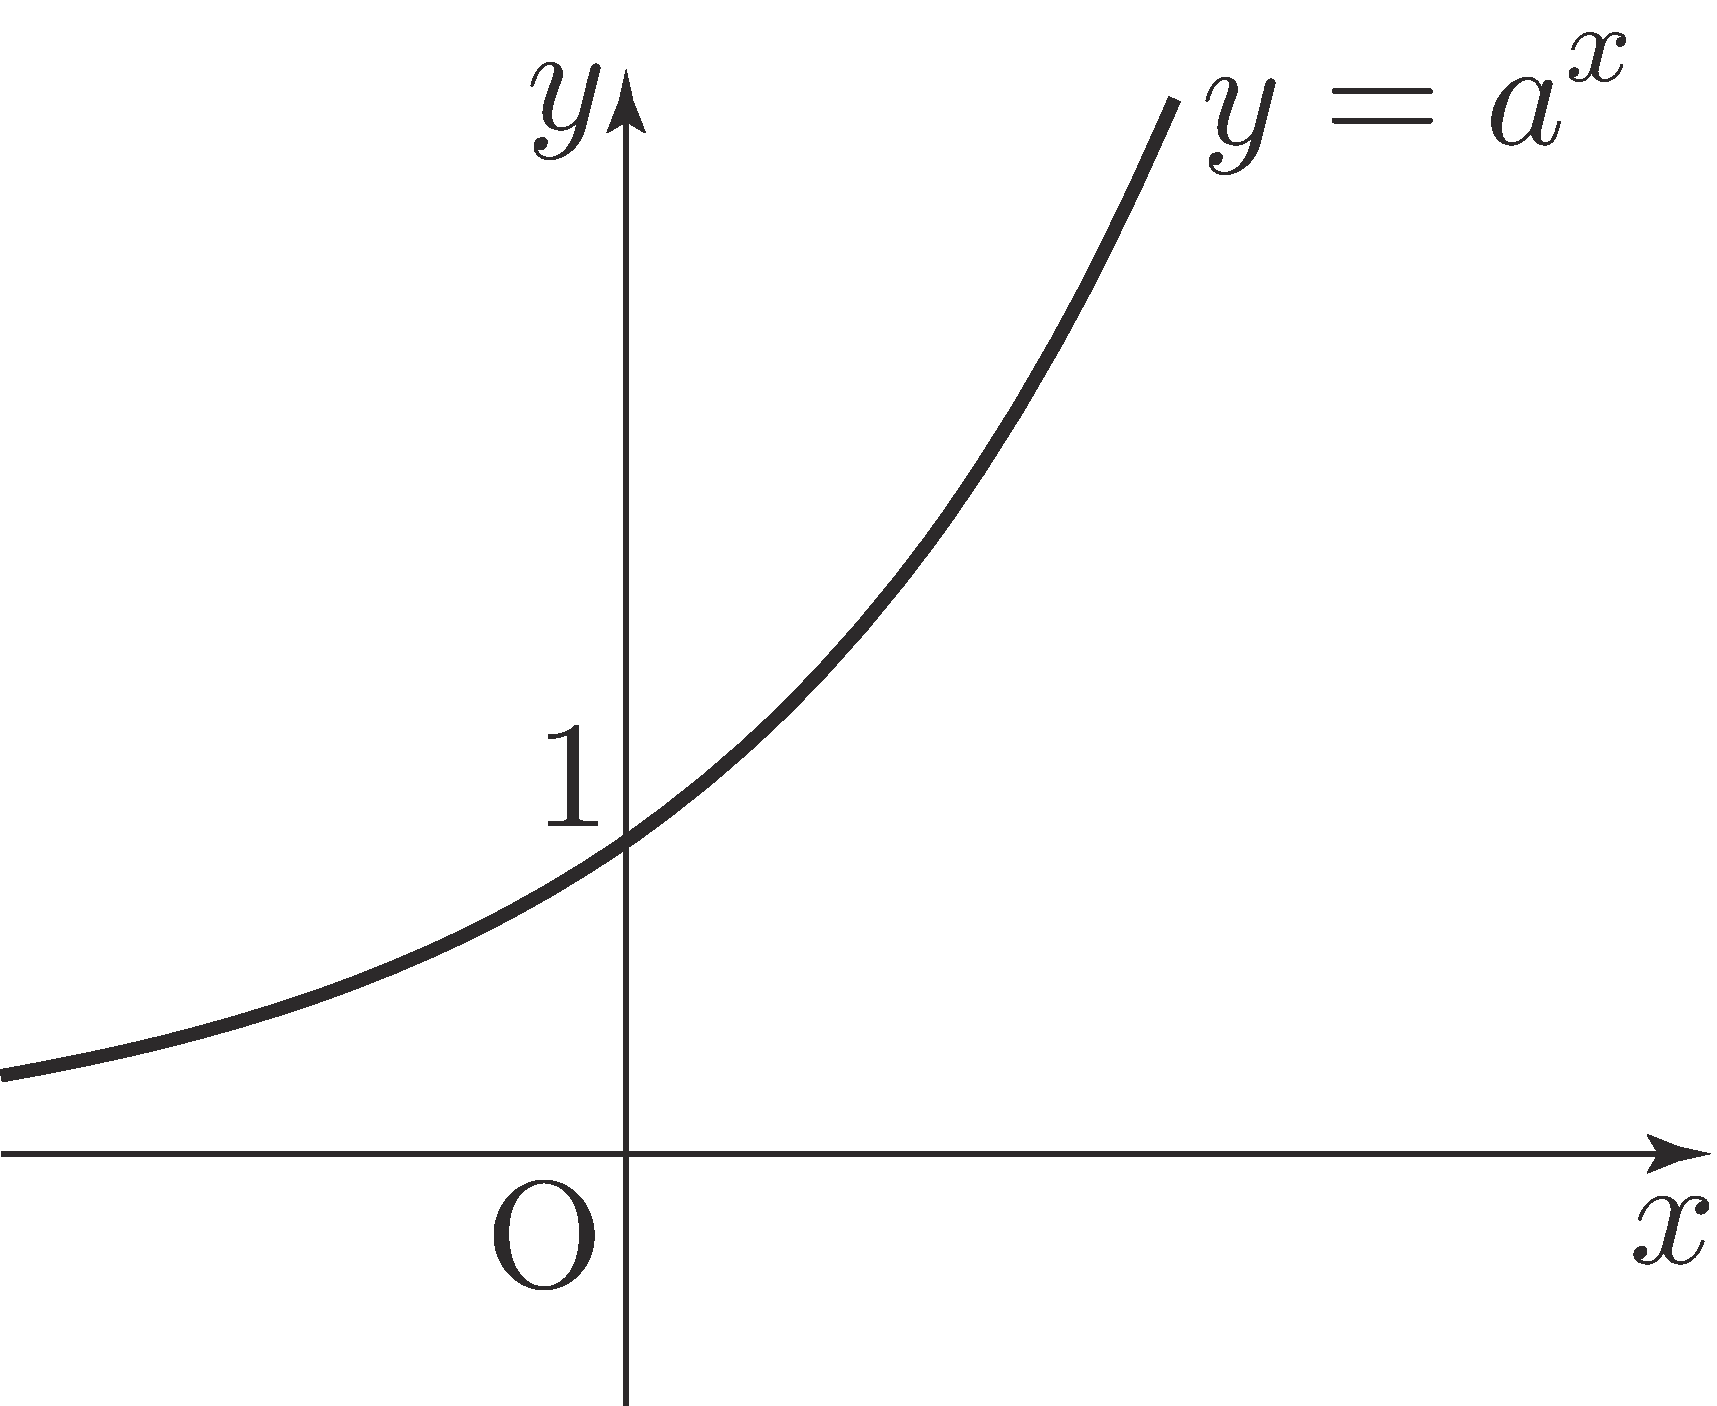
\includegraphics[scale=\pgfkeysvalueof{picsize}]{DBs/pic/zert_01_1.pdf}}\
\qquad\qquad
\centering \subfloat[][]{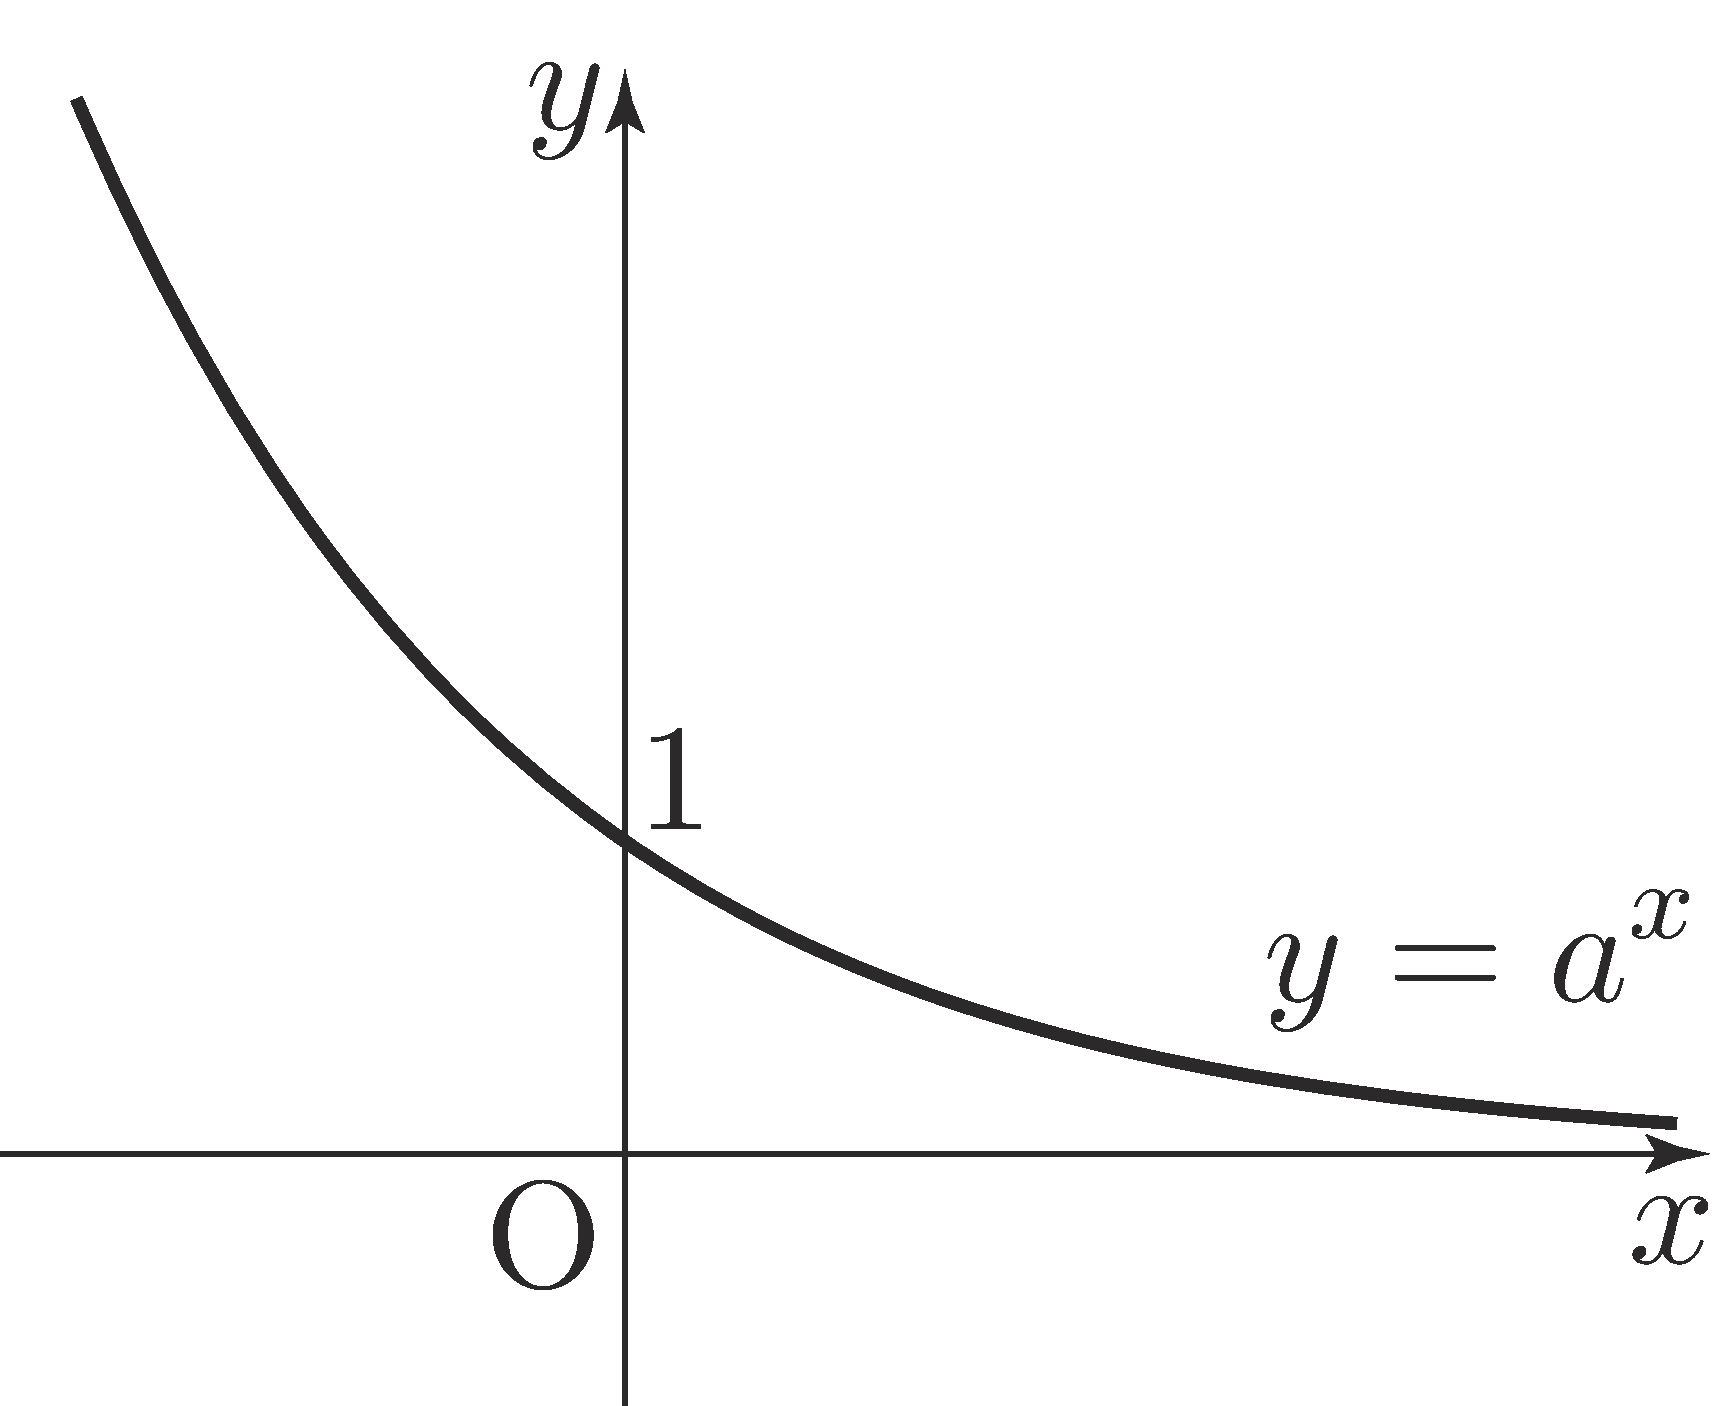
\includegraphics[scale=\pgfkeysvalueof{picsize}]{DBs/pic/zert_01_2.pdf}}\
\end{figure}


지수함수 $y=a^x$에서 $x=0$을 대입하면 $a$의 값에 관계 없이 $y=1$이므로, 지수함수의 그래프는 $a$의 값에 관계 없이 $\xy{0}{1}$을 지납니다. $a>1$이면 (a)와 같고, $0<a<1$이면 (b)와 같습니다.

\begin{figure}[h]
	\centering \subfloat[][]{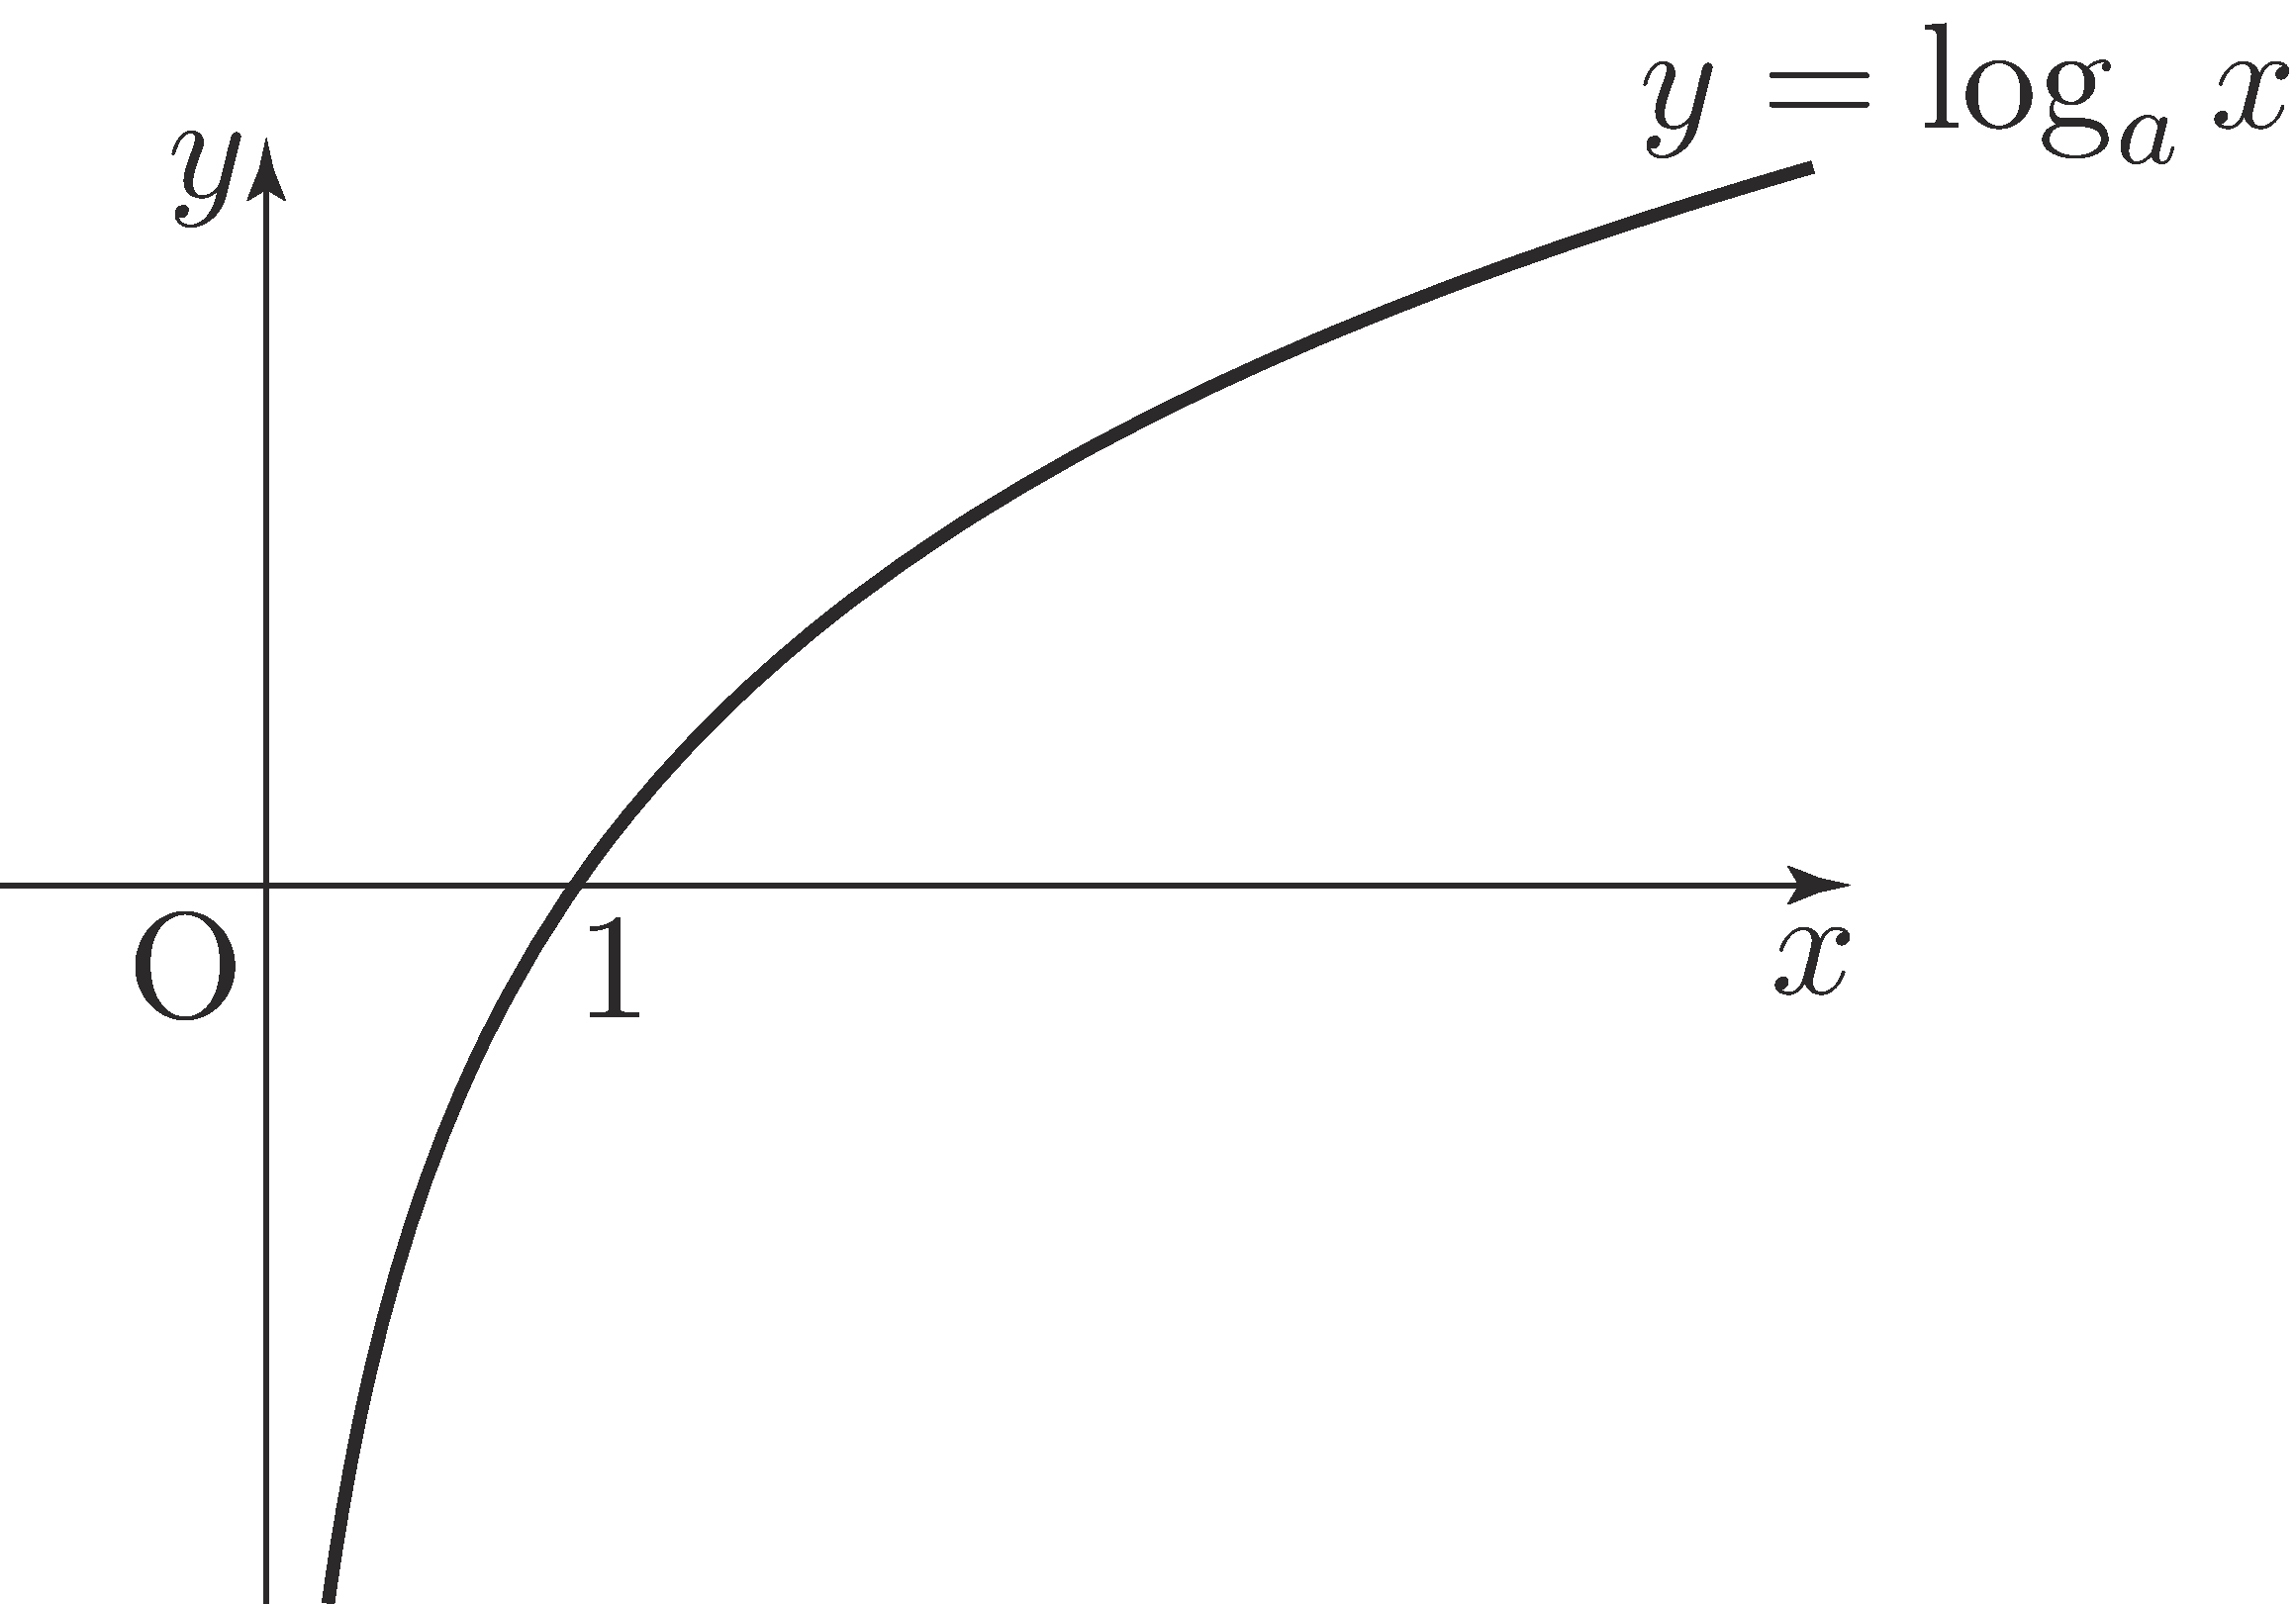
\includegraphics[scale=\pgfkeysvalueof{picsize}]{DBs/pic/zert_02_1.pdf}}\
	\qquad\qquad
	\centering \subfloat[][]{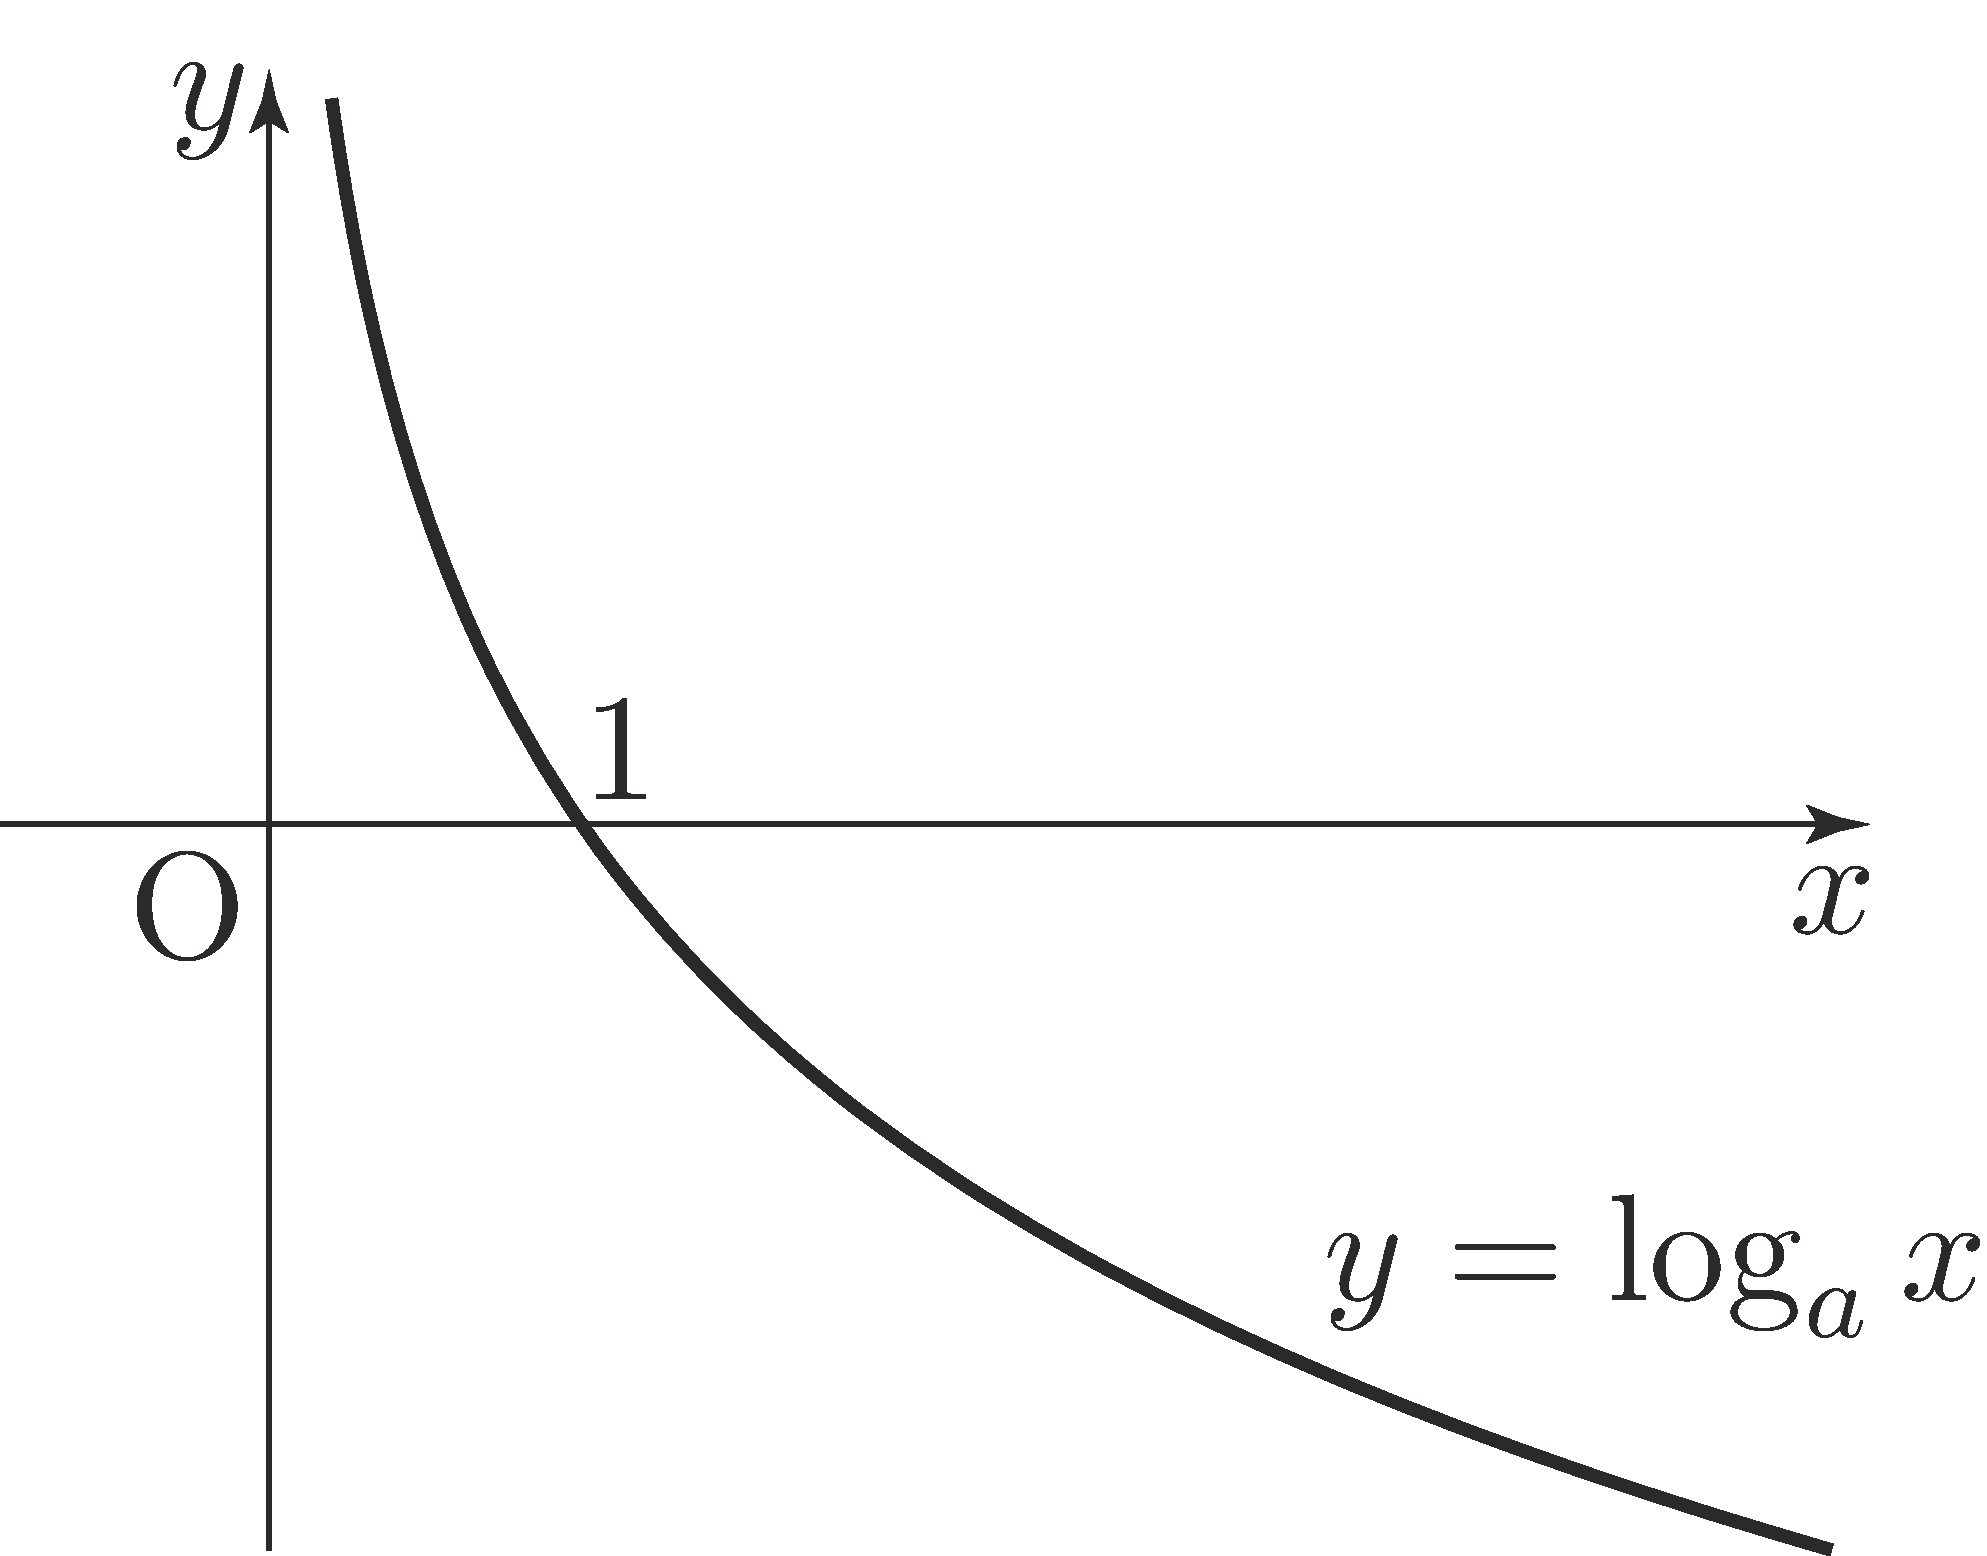
\includegraphics[scale=\pgfkeysvalueof{picsize}]{DBs/pic/zert_02_2.pdf}}\
	\end{figure}


로그함수 $y=\log_a x$에서 $x=1$을 대입하면 $a$의 값에 관계 없이 $y=0$이므로, 로그함수의 그래프는 $a$의 값에 관계 없이 $\xy{1}{0}$을 지납니다. $a>1$이면 (a)와 같고, $0<a<1$이면 (b)와 같습니다.

\begin{figure}[h]
	\centering \subfloat[][]{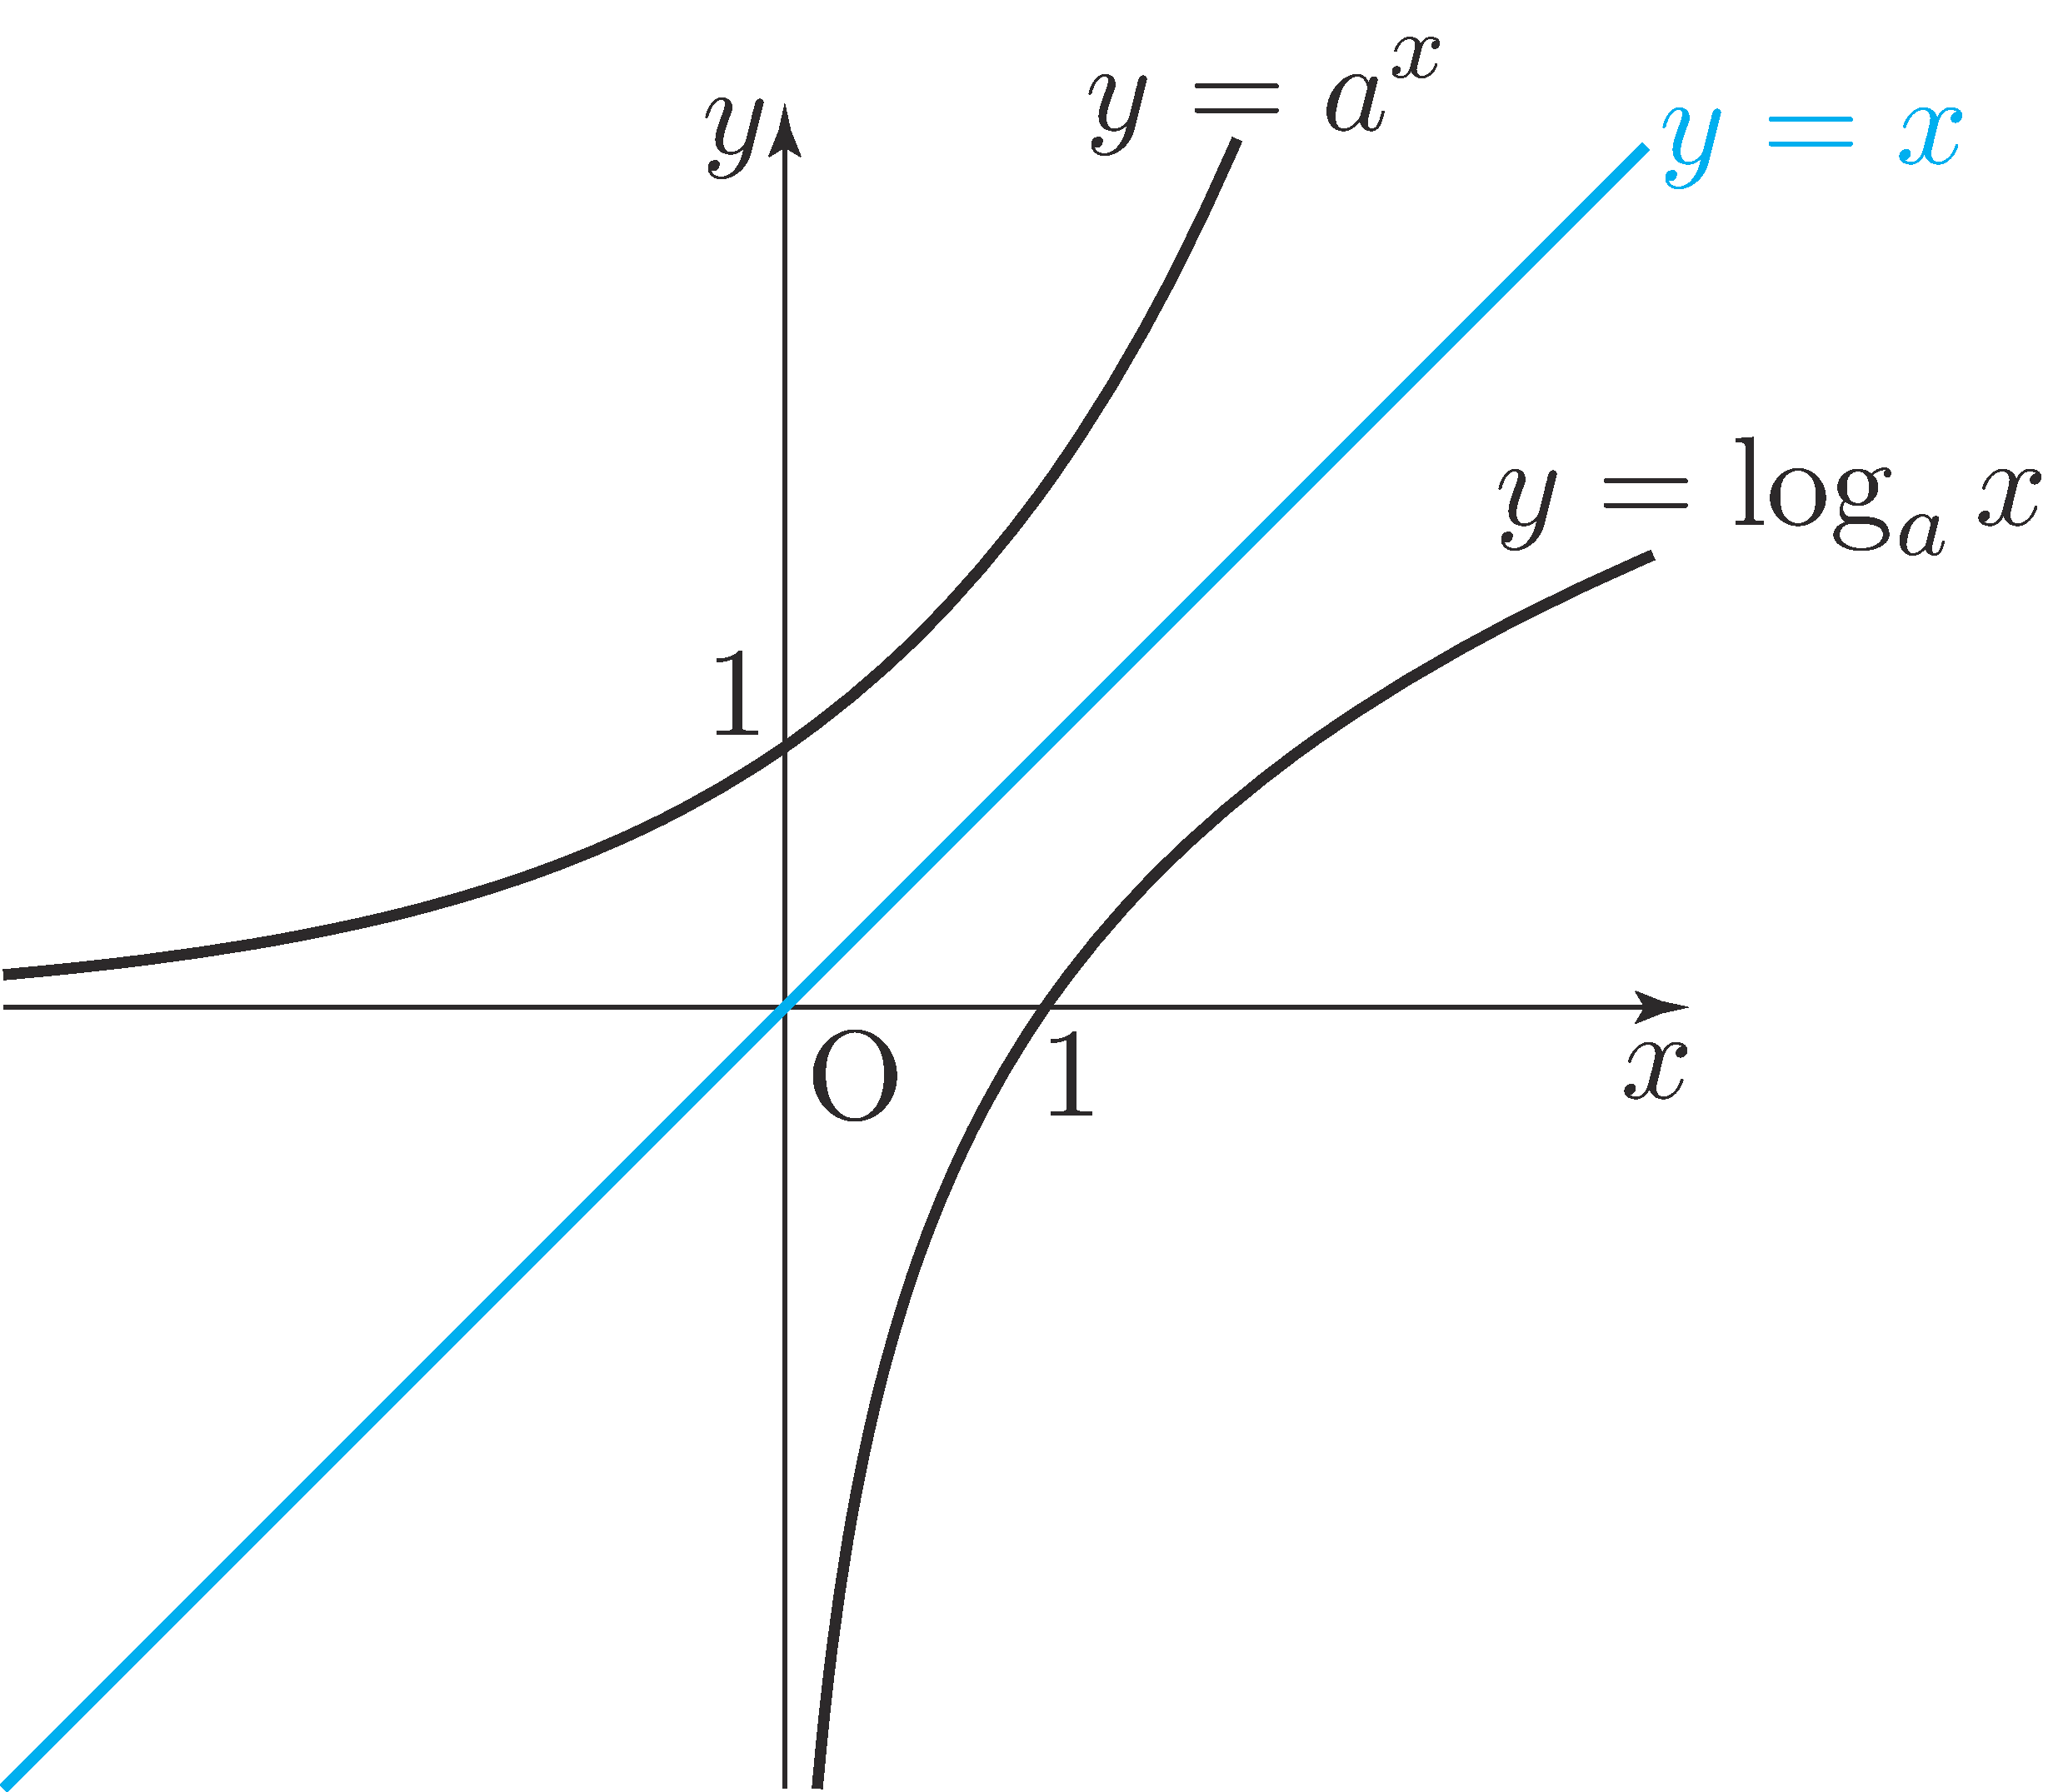
\includegraphics[scale=\pgfkeysvalueof{picsize}]{DBs/pic/zert_03_1.pdf}}\
	\qquad
	\centering \subfloat[][]{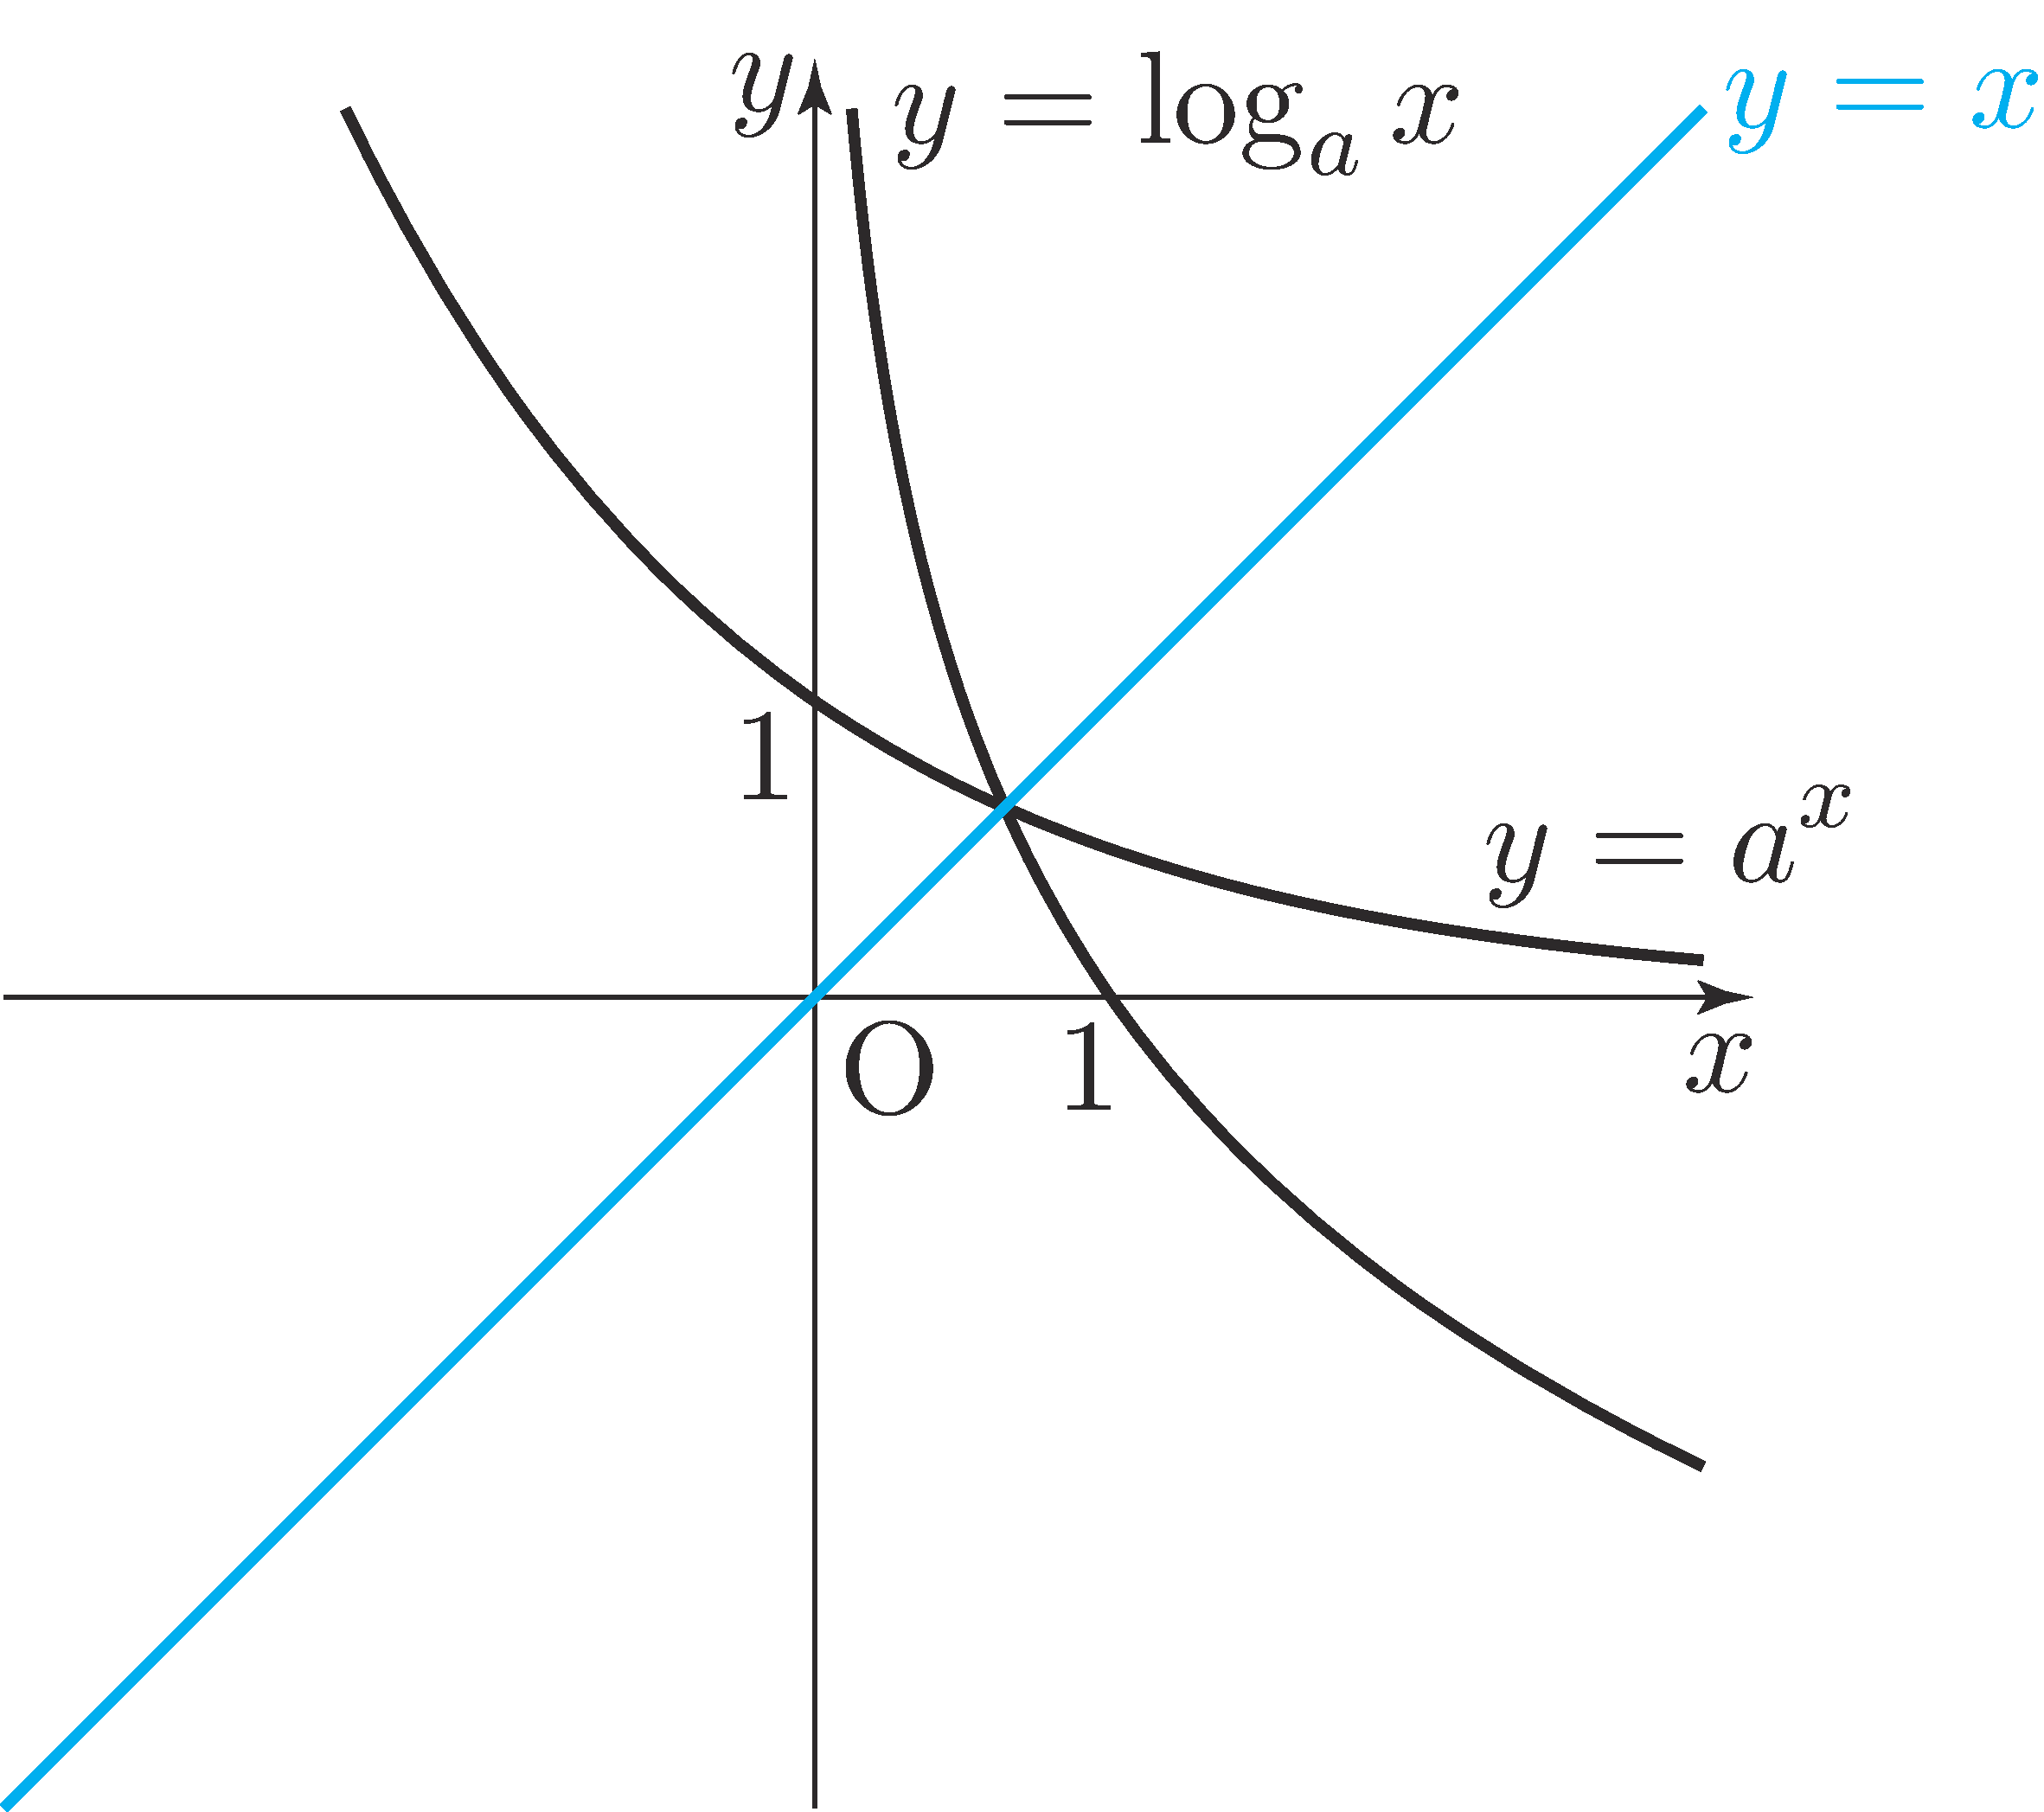
\includegraphics[scale=\pgfkeysvalueof{picsize}]{DBs/pic/zert_03_2.pdf}}\
	\end{figure}


지수함수와 로그함수는 서로 역함수 관계이므로 두 함수의 그래프는 직선 $y=x$에 대하여 대칭입니다. $a>1$이면 (a)와 같고, $0<a<1$이면 (b)와 같습니다.\mn[-5\blskip]{교과서에는 이 그림만 실려 있기 때문에 지수함수의 그래프와 로그함수의 그래프의 위치관계가 항상 이 두 그림 중 하나라고 생각하기 쉽습니다. 그러나 더 많은 위치관계가 존재합니다. 이는 Math I에서 다룹니다.}{}

\clearpage
\mychapter{공통 삼각함수}{}
\section{일반각}
$360^\circ$를 초과하거나 $0^\circ$ 미만인 각을 정의할 수 있습니다.
\begin{center}
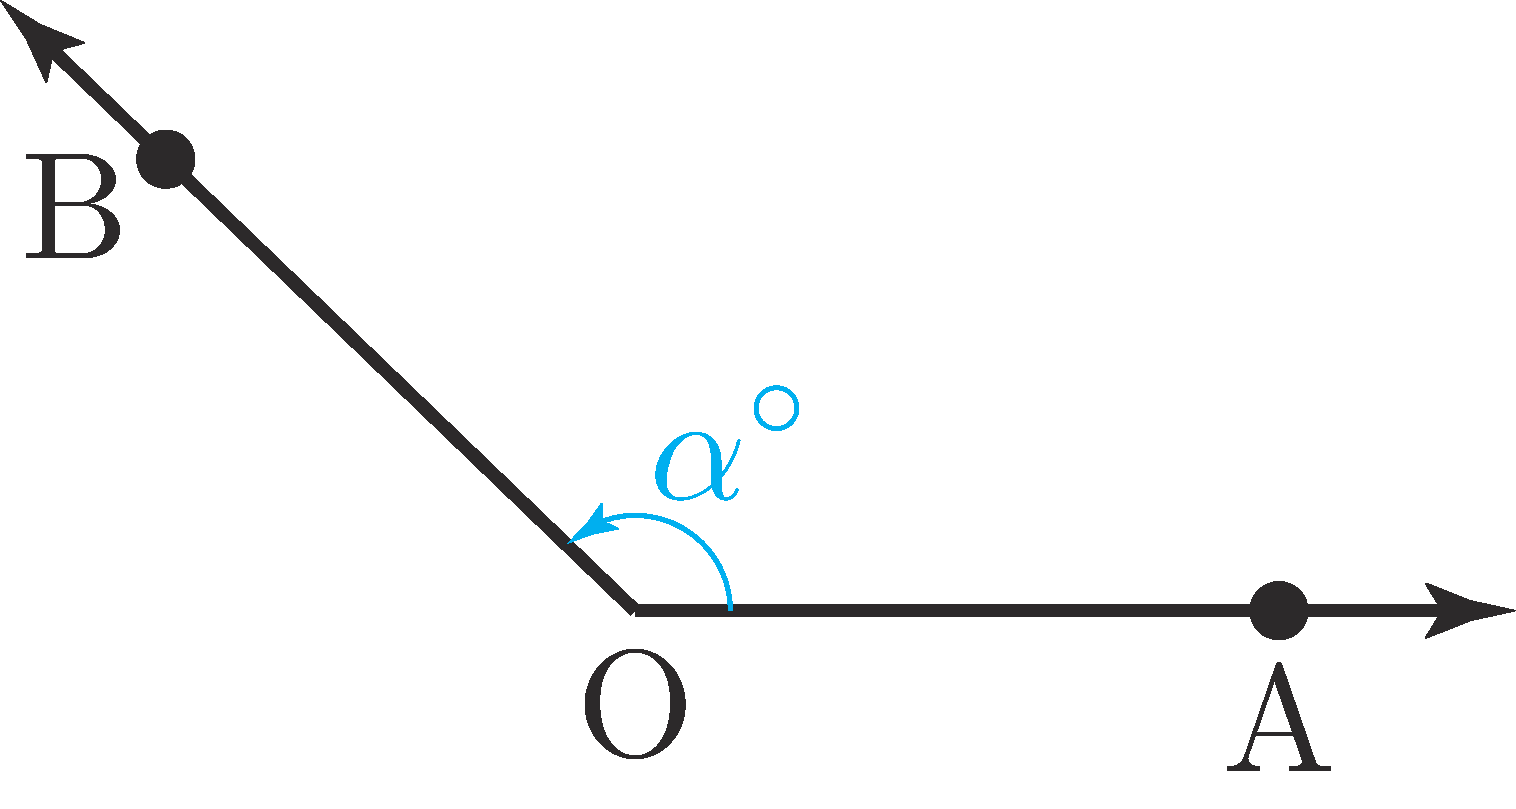
\includegraphics[scale=\pgfkeysvalueof{picsize}]{DBs/pic/zert_04.pdf}\
\end{center}$0 \le \alpha < 360$인 실수 $\alpha$에 대하여 각 $\mrm{AOB}$의 크기를 $\alpha^\circ$라 할 때, 각의 정의에 따르면 반직선 $\mrm{OA}$를 $\mrm{O}$를 중심으로 회전시켜 반직선 $\mrm{OB}$와 겹치게 할 수 있을 때 회전한 양이 $\alpha^\circ$입니다.
\begin{center}
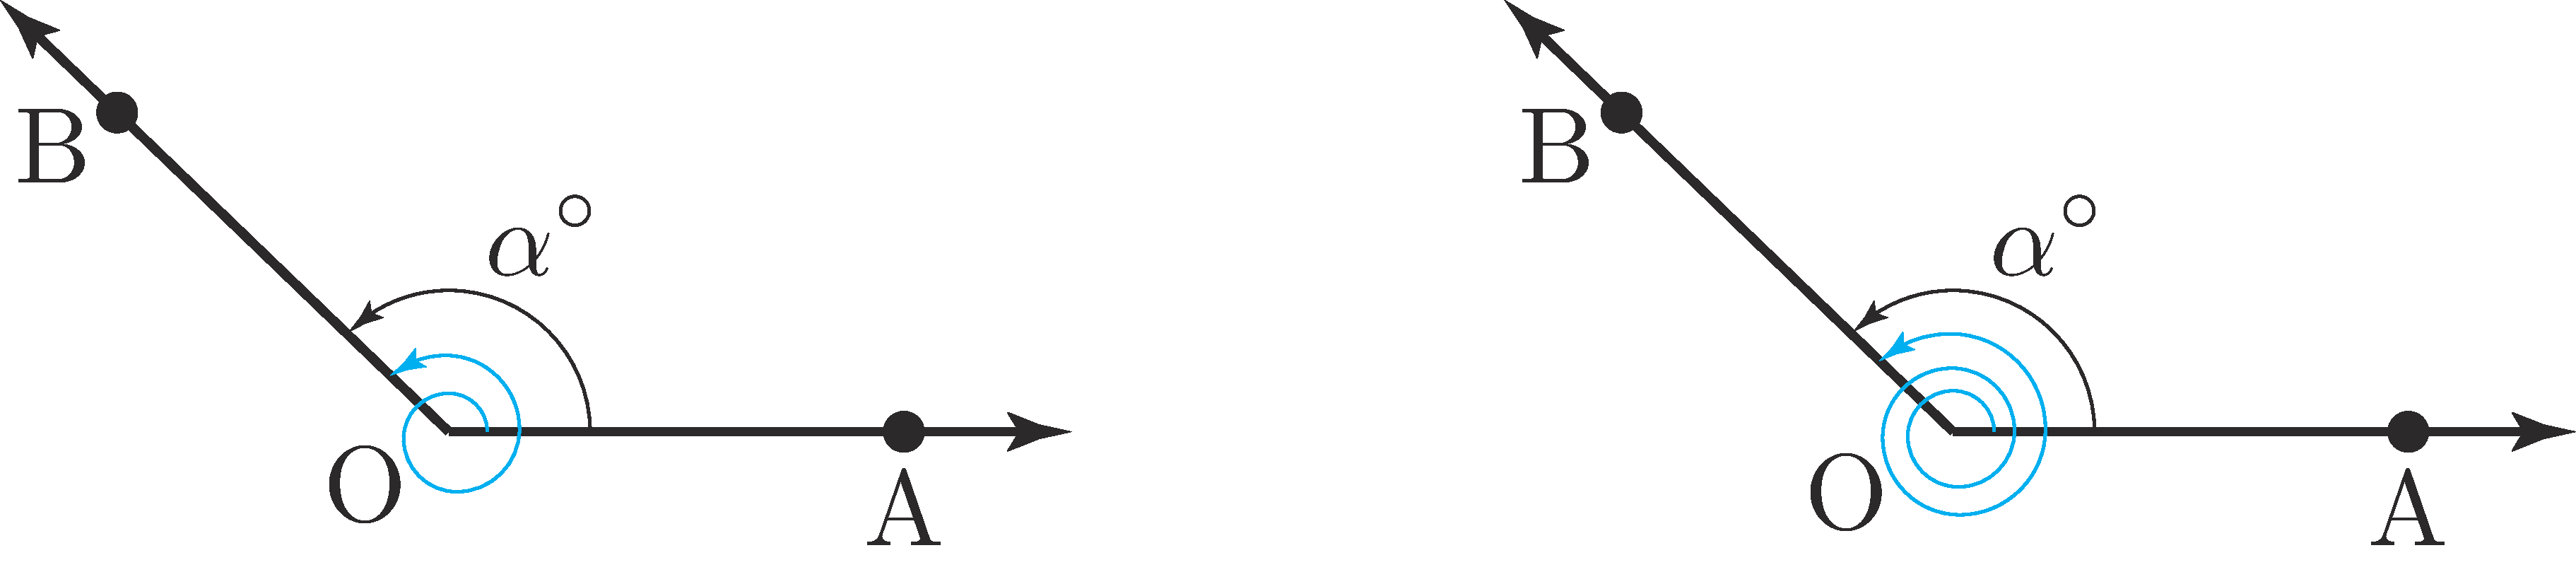
\includegraphics[scale=\pgfkeysvalueof{picsize}]{DBs/pic/zert_05.pdf}\
\end{center}그런데 $\alpha^\circ$만큼 회전한 후 같은 방향으로 한 바퀴를 더 돌아도, 즉 $\alpha^\circ + 360^\circ$만큼 회전하여도 반직선 $\mrm{OA}$를 반직선 $\mrm{OB}$와 겹치게 할 수 있습니다. 마찬가지로 모든 자연수 $n$에 대하여 $\alpha^\circ + n\times 360^\circ$만큼 회전하여도 반직선 $\mrm{OA}$를 반직선 $\mrm{OB}$와 겹치게 할 수 있습니다. 같은 방법으로 $\alpha^\circ$만큼 회전한 후 반대 방향으로 한 바퀴를 더 돌아도, 즉 $\alpha^\circ - 360^\circ$만큼 회전하여도 반직선 $\mrm{OA}$를 반직선 $\mrm{OB}$와 겹치게 할 수 있습니다. 마찬가지로 모든 자연수 $n$에 대하여 $\alpha^\circ - n\times 360^\circ$만큼 회전하여도 반직선 $\mrm{OA}$를 반직선 $\mrm{OB}$와 겹치게 할 수 있습니다.

이런 방법으로 모든 정수 $n$에 대하여 각 $\mrm{AOB}$의 크기를 $\alpha^\circ + n\times 360^\circ$라 나타낼 수 있습니다. 이때 시계 반대 방향으로 회전하는 것을 양의 방향 $(+)$, 시계 방향으로 회전하는 것을 음의 방향 $(-)$이라 하고, 이렇게 확장된 각의 정의를 \term{일반각}{}이라 합니다.

\section{호도법}
\begin{center} 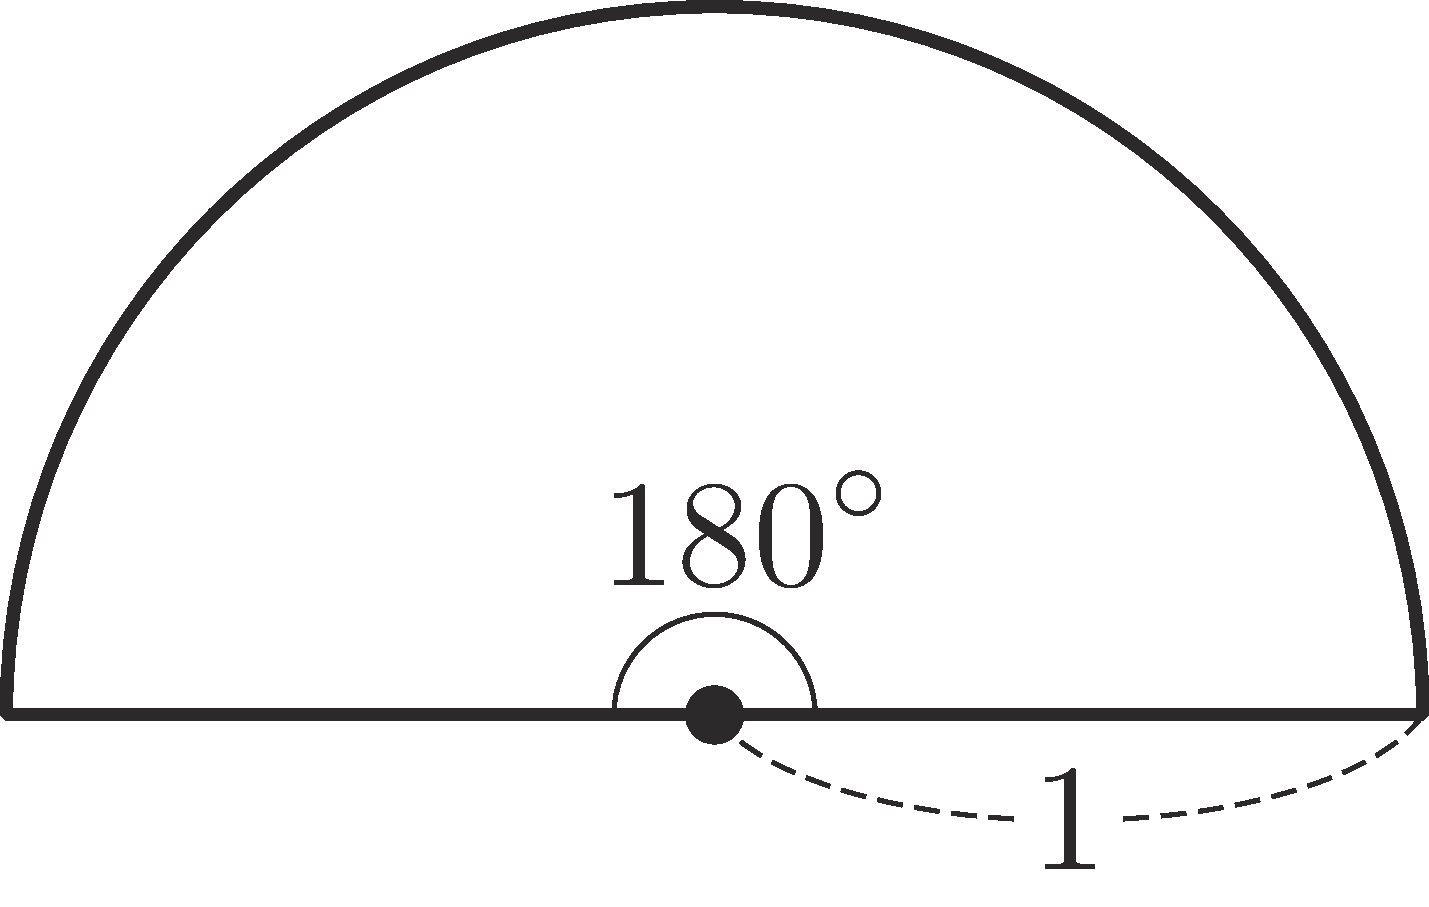
\includegraphics[scale=\pgfkeysvalueof{picsize}]{DBs/pic/zert_06.pdf}\
	\end{center}부채꼴에서 호의 길이는 중심각과 정비례하므로, 호의 길이를 이용하여 각도를 표시하는 단위를 생각할 수 있습니다. 반지름이 $1$이고 중심각이 $180^\circ$인 부채꼴, 즉 반원의 호의 길이는 $\pi$입니다. 이때 이 `호의 길이'를 그대로 `각의 크기'로 사용하는, 즉 `반원의 중심각은 $\pi$'와 같이 호의 길이를 각도의 크기에 대응시키는 방법이 \term{호도법}{}입니다.

호도법에서의 각도의 단위를 \term{라디안}{}이라 합니다. 호도법을 쓸 때에는 일반적으로 단위인 `라디안'을 생략하고 적습니다. 호도법을 이용하여 자주 사용되는 각의 크기를 나타내면 $30^\circ = \dfrac{\pi}{6}$, $45^\circ=\dfrac{\pi}{4}$, $60^\circ = \dfrac{\pi}{3}$, $90^\circ=\dfrac{\pi}{2}$, $360^\circ=2\pi$와 같습니다. 
\begin{center} 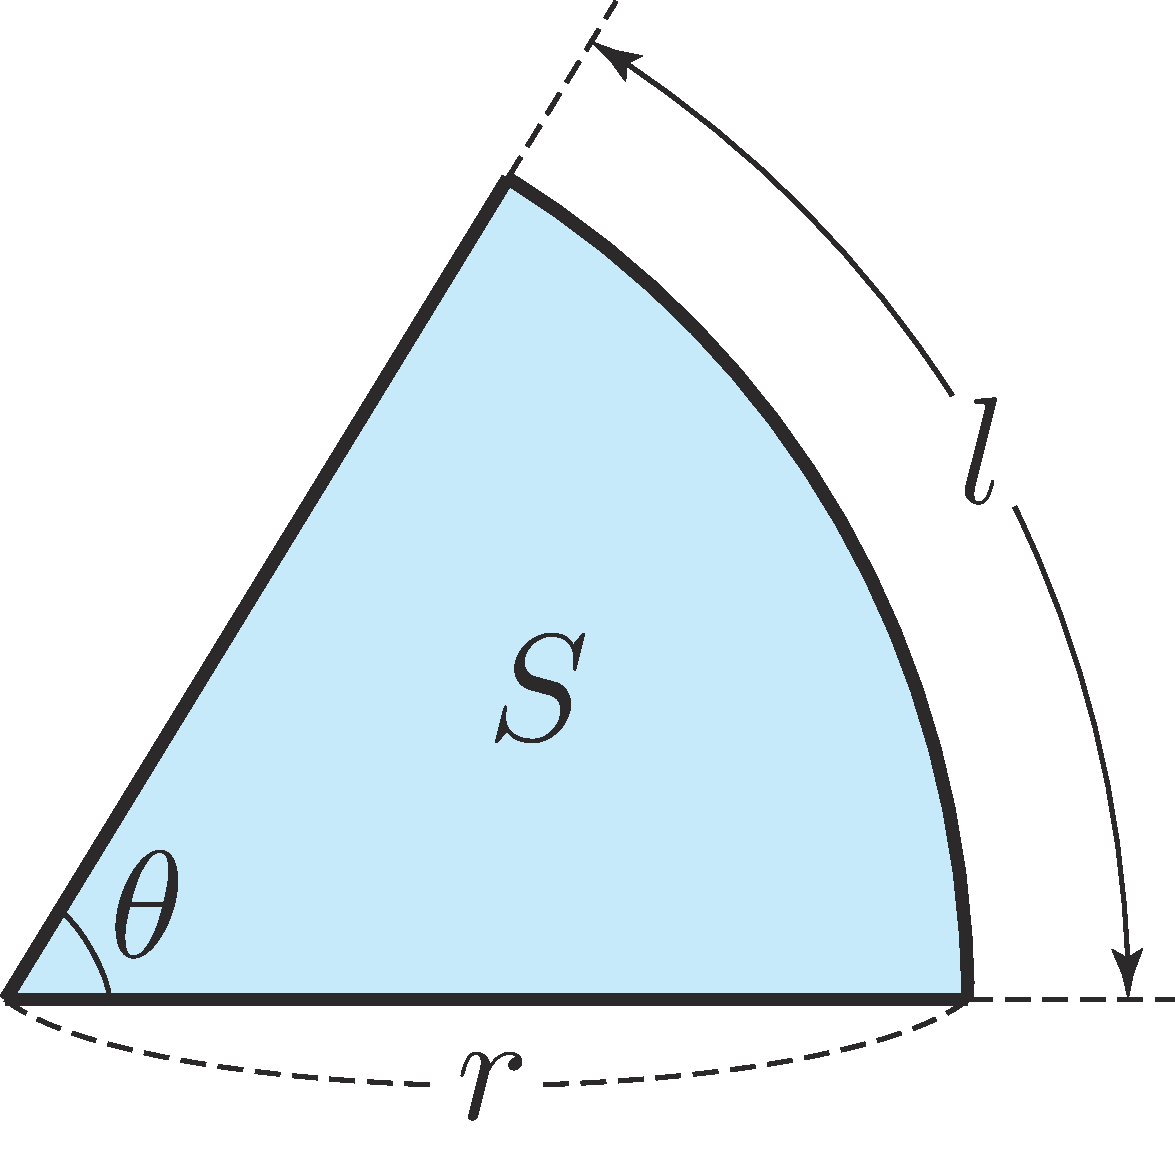
\includegraphics[scale=\pgfkeysvalueof{picsize}]{DBs/pic/zert_07.pdf}\
	\end{center}호도법을 이용하면 호의 길이, 부채꼴의 넓이를 구할 때 $\dfrac{\text{중심각의 크기}^\circ}{360^\circ}$를 사용하지 않고 쉽게 구할 수 있습니다. 예를 들어 중심각의 크기가 $\theta$이고 반지름의 길이가 $r$인 부채꼴에서 호의 길이 $l$에 대하여 $l = r\theta$입니다. 또한 부채꼴의 넓이 $S$에 대하여 $S = \dfrac{1}{2}lr$이므로 $l = r\theta$를 대입하면 $S =\dfrac{1}{2}r^2\theta$입니다.\\[-2em]

\section{삼각비}
\begin{center}
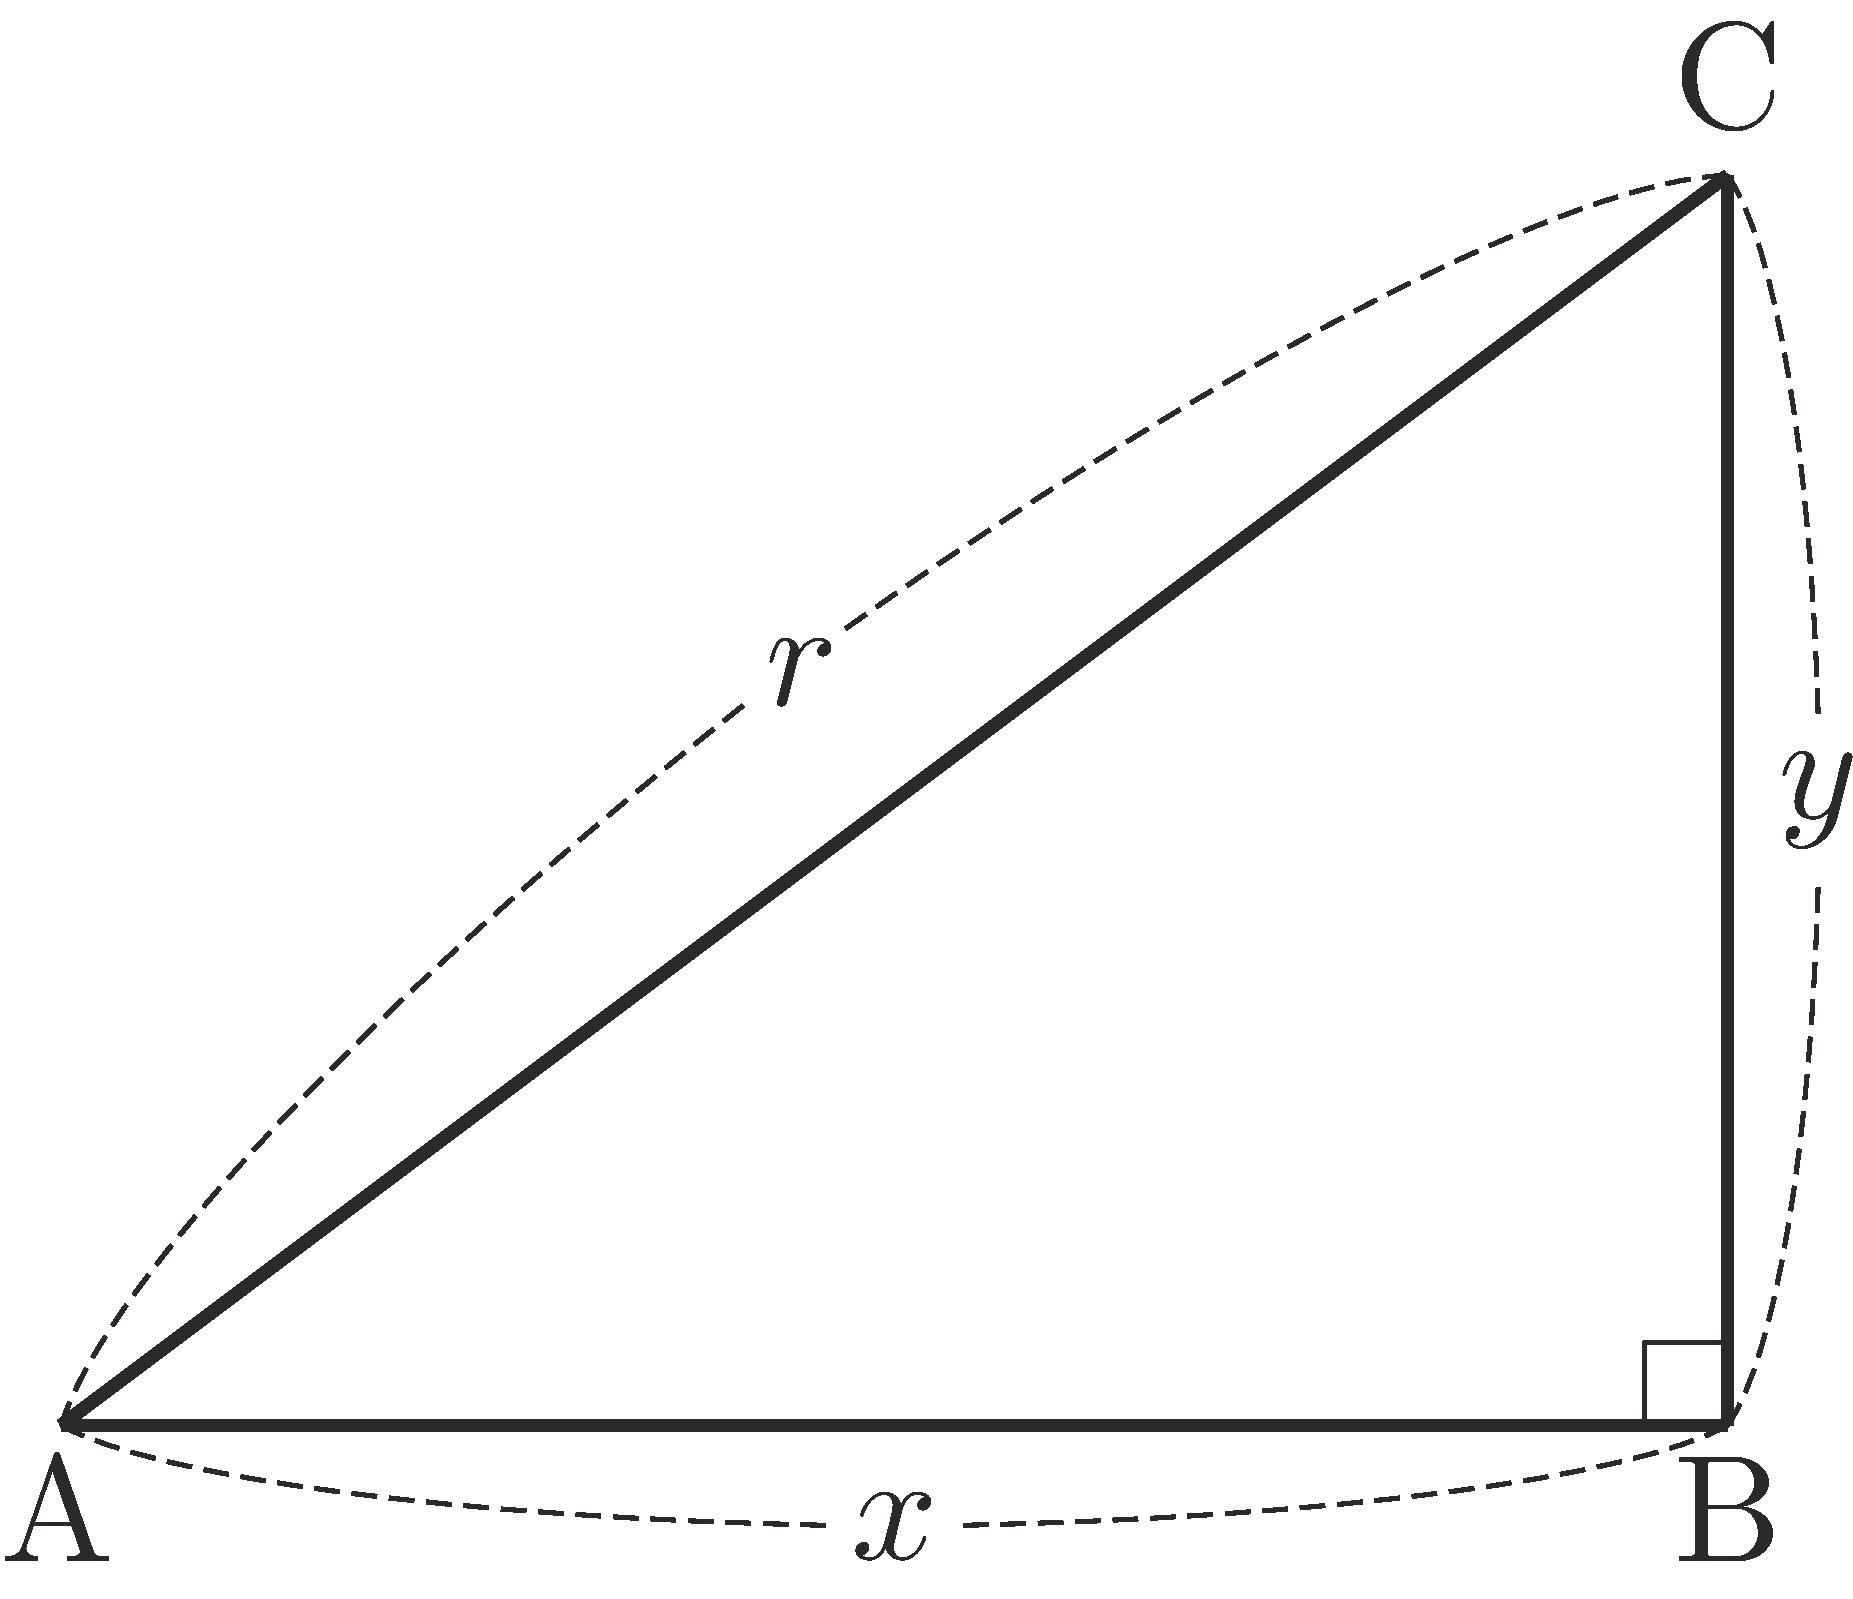
\includegraphics[scale=0.125]{pic0/pic154.pdf}
\end{center}$\angle \mrm{B} = 90^\circ$이고 $\ovr{AC}=r$, $\ovr{AB}=x$, $\ovr{BC}=y$인 직각삼각형 $\mrm{ABC}$에서 $\angle \mrm{A}$에 대한 \term{삼각비}{}인 \term{사인}{2}, \term{코사인}{}, \term{탄젠트}{}를 다음과 같이 정의합니다.
\begin{align*} 
\sin \angle \mrm{A} = \dfrac{y}{r},\quad
\cos \angle \mrm{A} = \dfrac{x}{r},\quad
\tan \angle \mrm{A} = \dfrac{y}{x} 
\end{align*}

\section{삼각함수}
\begin{center}
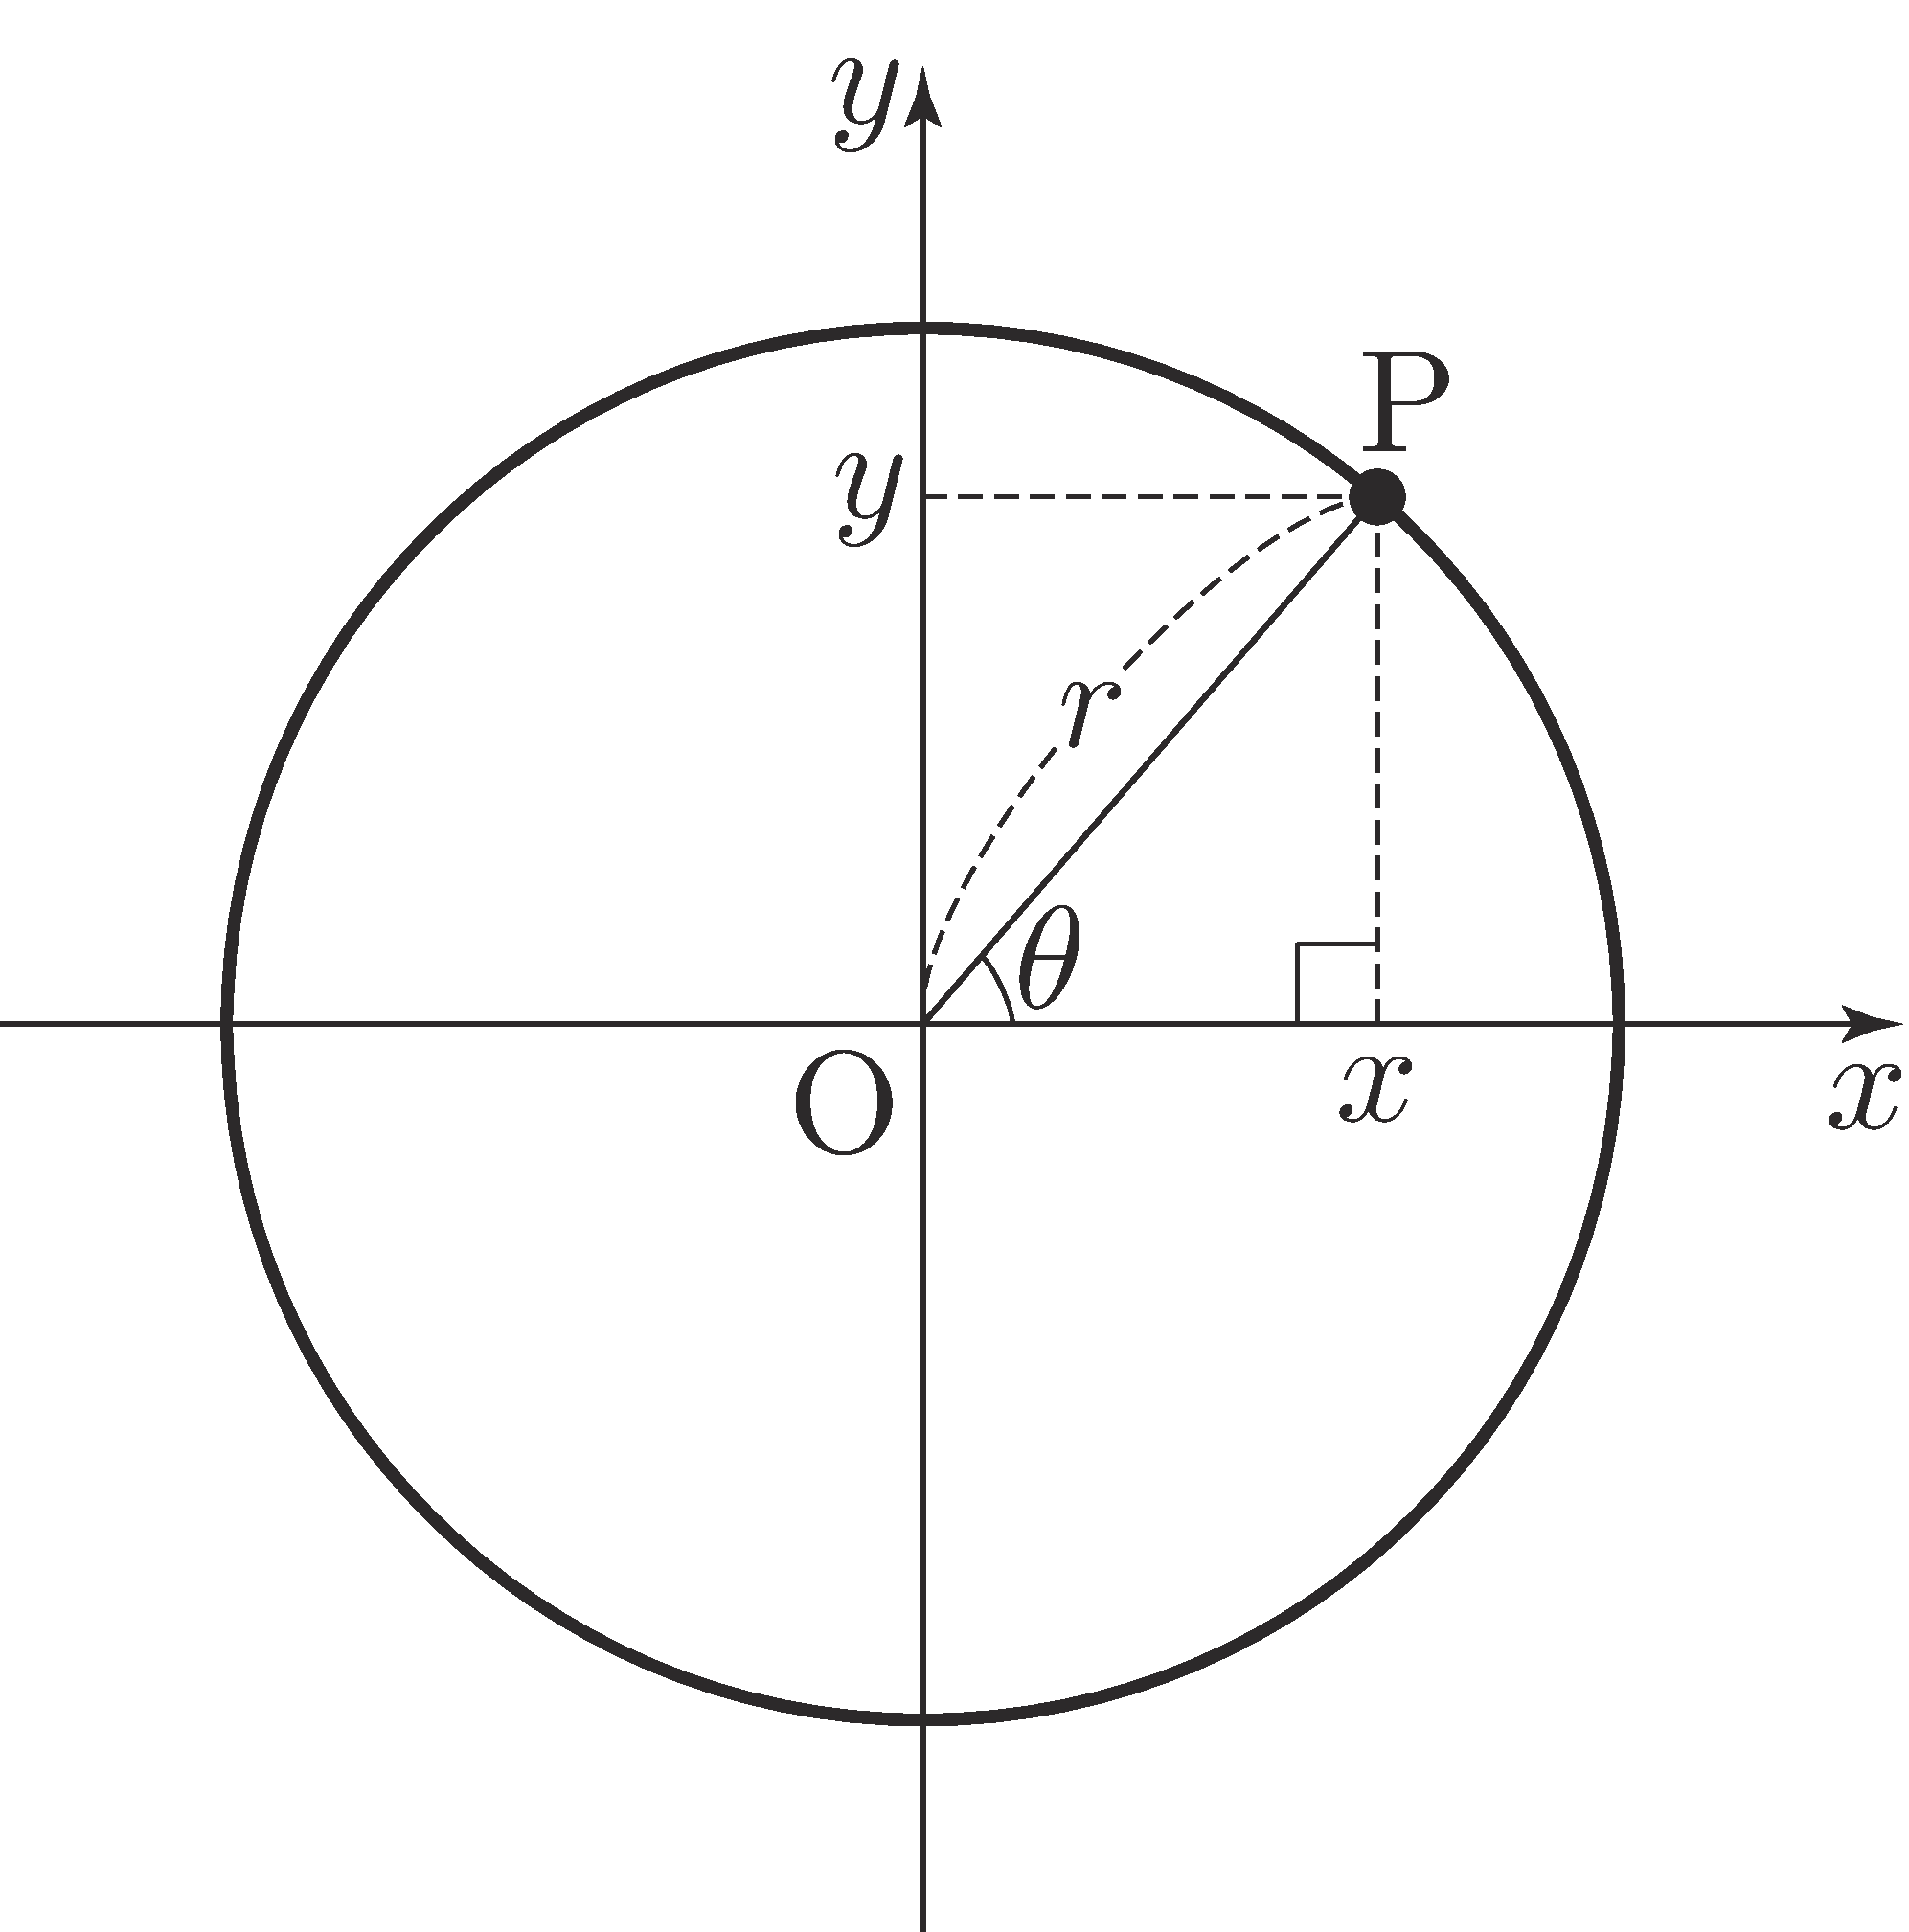
\includegraphics[scale=0.125]{pic0/pic155.pdf}
\end{center}좌표평면에서 중심이 원점 $\mrm{O}$이고 반지름의 길이가 $r$인 원 위의 점 $\xy[P]{x}{y}$에 대하여 직선 $\mrm{OP}$와 $x$축이 이루는 일반각을 $\theta$라 할 때, $\theta$에 대한 \term{삼각함수}{}인 \term{사인함수}{}, \term{코사인함수}{}, \term{탄젠트함수}{}를 다음과 같이 정의합니다.\mn{이때 $x$가 분모에 들어갈 때에는 $0$이 아니어야 합니다.}{}
\begin{align*}
  \sin \theta = \dfrac{y}{r},\quad
  \cos \theta = \dfrac{x}{r},\quad
  \tan \theta = \dfrac{y}{x}
\end{align*}
\clearpage
\subsection{삼각함수 사이의 관계}\term[삼각함수]{삼각함수 사이의 관계}{0}
$\tan\theta =\dfrac{y}{x} = \dfrac{\qfrac{y}{r}}{\qfrac*{x}{r}} =\dfrac{\sin\theta}{\cos\theta}$이므로 $\tan\theta=\dfrac{\sin\theta}{\cos\theta}$가 성립합니다. 한편 $\sin^2 \theta + \cos^2 \theta = \dfrac{x^2+y^2}{r^2} = 1$이므로 $\sin^2 \theta + \cos^2 \theta = 1$이 성립합니다.

\subsection{사인함수, 코사인함수, 탄젠트함수의 그래프}
\begin{center}
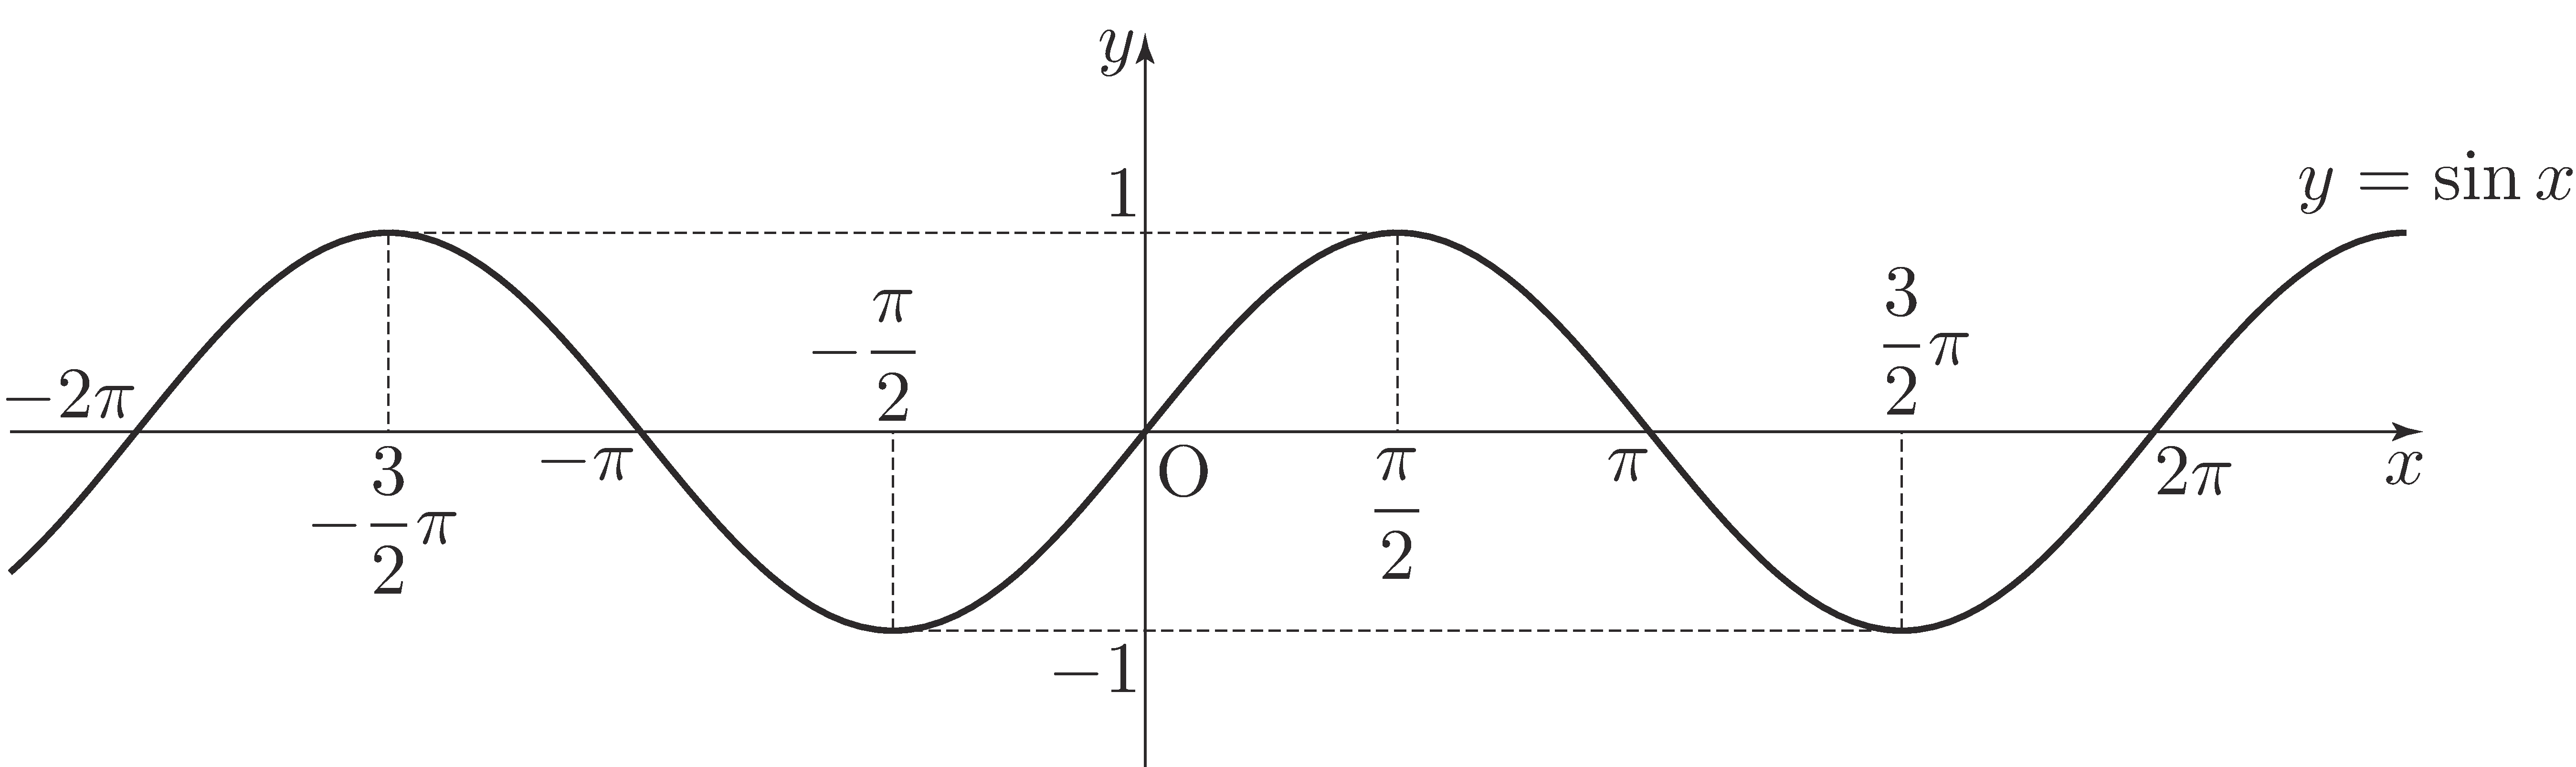
\includegraphics[scale=0.125]{pic0/pic156.pdf}
\end{center}사인함수 $y=\sin x$의 그래프는 위 그림과 같고, 원점에 대하여 대칭이며, 주기가 $2\pi$입니다.\term[사인함수]{사인함수의 그래프}{0}\mn{대칭, 주기 등의 용어에 대한 설명은 Graph에서 다룹니다.}{}
\begin{center}
\includegraphics[scale=0.125]{pic0/pic157.pdf}
\end{center}코사인함수 $y=\cos x$의 그래프는 위 그림과 같고, $y$축에 대하여 대칭이며, 주기가 $2\pi$입니다.\term[코사인함수]{코사인함수의 그래프}{0}
\begin{center}
\includegraphics[scale=0.125]{pic0/pic158.pdf}
\end{center}탄젠트함수 $y=\tan x$의 그래프는 위 그림과 같고, 원점에 대하여 대칭이며, 주기가 $\pi$입니다.\term[탄젠트함수]{탄젠트함수의 그래프}{0}
\clearpage
\section{삼각함수의 활용}\term[선분!선분의 길이]{삼각함수를 이용하기}{0}
\subsection{선분의 길이를 삼각함수를 이용하여 나타내기}
\begin{center}
\includegraphics[scale=0.125]{pic0/pic159.pdf}
\end{center}그림과 같이 $\angle \mrm{C} = \dfrac{\pi}{2}$, $\angle \mrm{B} = \theta$인 직각삼각형에서 $a = c\times \cos\theta$, $b = c\times \sin\theta$, $b = a\times\tan\theta$ 등과 같이 선분의 길이를 삼각함수를 이용하여 나타낼 수 있습니다.

\subsection{사인법칙}\begin{center}  \centering \includegraphics[scale=0.125]{pic0/pic164.pdf}\\
  \end{center}외접원의 반지름의 길이가 $R$인 삼각형 $\mrm{ABC}$에서 $\dfrac{a}{\sin A}=\dfrac{b}{\sin B}=\dfrac{c}{\sin C}=2R$이 성립합니다.\mn{다음과 같은 꼴로 암기하면 세 변의 길이를 즉각 이용할 수 있습니다.\begin{align*}
a &= 2R\sin A \\ 
b &= 2R\sin B \\
c &= 2R\sin C
\end{align*}
}{}
\subsection{코사인법칙}

\begin{figure}[h]
  \centering \includegraphics[scale=0.125]{pic0/pic165.pdf}\\
  \end{figure}
삼각형 $\mrm{ABC}$에서 다음이 성립합니다.
\begin{align*}
a^2 &= b^2 + c^2 - 2bc\cos A \\ 
b^2 &= c^2 + a^2 - 2ca\cos B \\
c^2 &= a^2 + b^2 - 2ab\cos C
\end{align*}
\clearpage
\subsection{삼각형의 넓이}\term[넓이!삼각형]{삼각함수를 이용하기}{0}
\begin{center}
\includegraphics[scale=0.125]{pic0/pic160.pdf}
\end{center}두 변의 길이가 $a$, $b$이고 그 끼인각의 크기가 $\theta$인 삼각형의 넓이는 $\dfrac{1}{2}ab\sin\theta$입니다. 이는 `$a$를 밑변으로 보고 $b\sin\theta$를 높이로 본 것' 또는 `$b$를 밑변으로 보고 $a\sin\theta$를 높이로 본 것'입니다.

\begin{figure}[h]
  \centering \includegraphics[scale=0.125]{pic0/pic166.pdf}\\
  \end{figure}
이는 $\theta$가 직각이거나 둔각이어도 마찬가지입니다.

 
\mychapter{수열}{}
\section{수열의 정의}
\subsection{문장으로 정의}
차례로 나열된 수의 열을 \term{수열}{}이라 하고, 나열된 각각의 수를 그 수열의 \term[수열]{항}{2}이라고 합니다. 일반적으로 수열을 다음과 같이 나타냅니다.
\begin{align*}a_1,\:a_2,\:a_3 ,\: \cdots,\: a_n,\:\cdots\end{align*}
이때 앞에서부터 차례로 제$1$항, 제$2$항, 제$3$항, $\cdots$, 제$n$항, $\cdots$이라고 합니다.
\subsection{함수로 정의}
$\mathbb N$의 원소 $n$과 수열의 항 $a_n$을 대응시키면 이 대응은 $\mathbb N$에서 $\mathbb R$로의 함수로 생각할 수 있습니다. 즉, 다음과 같습니다.
\begin{align*} f : \mathbb N \longrightarrow \mathbb R, \: f(n)=a_n\end{align*}
\subsection{일반항}
함수식 $f(n)$을 $n$에 대한 식으로 나타내면, 그 식의 $n$에 적절한 자연수를 대입하여 수열의 각 항을 구할 수 있습니다. 그런데 $f(n)=a_n$이므로, 제$n$항 $a_n$이 수열의 각 항을 일반적으로 나타내고 있음을 알 수 있습니다. 이러한 의미에서 제$n$항 $a_n$을 이 수열의 \term{일반항}{}이라고 하며, 일반항이 $a_n$인 수열을 간단히 $\left\{ a_n \right\} $과 같이 나타냅니다.
\section{등차수열과 등비수열}
\subsection{정의, 관계식, 일반항}
첫째항부터 차례로 일정한 수를 더하여 만든 수열을 \term{등차수열}{}이라 하고, 더하는 일정한 수를 \term{공차}{}라고 합니다. 공차가 $d$인 등차수열 $\left\{ a_n \right\} $에서 $a_n$에 공차 $d$를 더하면 $a_{n+1}$이 되므로 $a_{n+1} = a_n + d$가 성립합니다. 이를 이용하여 등차수열의 일반항을 구하면 $a_n = a + \left( n-1 \right) d$입니다.

첫째항부터 차례로 일정한 수를 곱하여 만든 수열을 \term{등비수열}{}이라 하고, 곱하는 일정한 수를 \term{공비}{}라고 합니다. 공비가 $r$인 등비수열 $\left\{ a_n \right\} $에서 $a_n$에 공비 $r$를 곱하면 $a_{n+1}$이 되므로 $a_{n+1} = a_nr$가 성립합니다. 이를 이용하여 등비수열의 일반항을 구하면 $a_n = ar^{n-1}$입니다.
\clearpage
\subsection{중항, 산술평균, 기하평균}
세 수 $a$, $b$, $c$가 이 순서대로 등차수열을 이룰 때, $2b=a+c$가 성립하며, $b$를 $a$와 $c$의 \term{등차중항}{}이라고 합니다. 세 수 $a$, $b$, $c$가 이 순서대로 등비수열을 이룰 때, $b^2 = ac$가 성립하며, $b$를 $a$와 $c$의 \term{등비중항}{}이라고 합니다.

등차중항 $\dfrac{a+c}{2}$는 $a$와 $c$의 \term{산술평균}{}이라고 하고, 두 등비중항 $\sqrt{ac}$, $-\sqrt{ac}$중에서 양수인 것을 $a$와 $c$의 \term{기하평균}{}이라고 합니다. $a$와 $c$가 모두 양수이면 산술평균과 기하평균에 대하여 다음이 항상 성립합니다. (단, 등호는 $a=c$일 때에만 성립) \begin{align*} \dfrac{a+c}{2} \ge \sqrt{ac}\end{align*}

\section{여러 가지 수열의 합}
\subsection{$\sum$의 정의}
수열 $\left\{ a_n \right\} $의 제$1$항부터 제$n$항까지의 \term[수열]{합}{2}을 $\sum_{k=1}^{n}a_k$라 표기합니다. 이는 $a_k$의 $k$에 $1$, $2$, $\cdots$, $n$을 차례로 대입하여 얻은 항들의 합을 의미합니다.

\subsection{$\sum$의 성질}
$\sum$는 합으로부터 정의되었으므로 다음과 같은 성질을 갖습니다.
\begin{thmbox}
    \begin{enumerate}[label=\onum*]
        \item $\sum_{k=1}^{n}\left( a_k + b_k\right) = \sum_{k=1}^{n}a_k + \sum_{k=1}^{n}b_k$
        \item $\sum_{k=1}^{n}\left( a_k - b_k\right) = \sum_{k=1}^{n}a_k - \sum_{k=1}^{n}b_k$
        \item $\sum_{k=1}^{n}ca_k = c\sum_
        {k=1}^{n}a_k$ (단, $c$는 상수)
        \item $\sum_{k=1}^{n}c = cn $(단, $c$는 상수)
    \end{enumerate}    
\end{thmbox}
\clearpage
\subsection{자연수의 거듭제곱의 합}
자연수의 거듭제곱의 합을 구하면 다음과 같습니다(증명 생략).
\begin{thmbox}
    \begin{enumerate}[label=\onum*]
        \item $\sum_{k=1}^{n}k = \dfrac{n\left( n+1 \right) }{2}$
    
        \item $\sum_{k=1}^{n}k^2 = \dfrac{n\left( n+1 \right)(2n+1) }{6}$ 
        \item $\sum_{k=1}^{n}k^3 = \left\{ \dfrac{n\left( n+1 \right) }{2} \right\}^2 $
    \end{enumerate}    
\end{thmbox}

\subsection{등차수열과 등비수열의 합}
등차수열 $\left\{ a_n \right\} $의 합 $\sum_{k=1}^{n}a_n$과 등비수열 $\left\{ b_n \right\} $의 합 $\sum_{k=1}^{n}b_n$은 각각 다음과 같습니다.
 \begin{align*}
    \sum_{k=1}^{n}a_n &= \dfrac{n\left( a_1 +a_n \right) }{2}
    = \dfrac{n\left( 2a_1+\left( n-1 \right)d  \right) }{2}\\ 
    \sum_{k=1}^{n}b_n &
    \begin{cases}
    = \dfrac{b_1\left( r^n -1 \right) }{r-1} = \dfrac{b_1\left( 1-r^n \right) }{1-r} & \text{(단,\:$r \ne 1$)}\\
    = nb_1 & \text{(단,\:$r  = 1$)}
    \end{cases}
 \end{align*}
\section{수학적귀납법}
일반적으로 명제 $p\left( n \right) $이 $n\ge m$ ($m$은 $1$ 이상의 자연수)인 모든 자연수 $n$에 대하여 성립함을 증명하려면 다음의 두 가지를 보이면 됩니다. 
\begin{thmbox}
\begin{enumerate}[label={\onum*}]
    \item $n=m$일 때 $p\left( n \right) $이 성립한다.
    \item $k\ge m$인 $k$에 대하여 $n=k$일 때 명제 $p\left( n \right) $이 성립한다고 가정하면, $n=k+1$일 때에도 명제 $p\left( n \right) $이 성립한다.
\end{enumerate}
\end{thmbox}
이렇게 증명하는 방법을 \term{수학적귀납법}{}이라고 합니다. 

\input{_COMMON/0-Zero24}
\cleartorecto\part{Zero 3) 함수 이후의 기본 개념}\cleartoverso

\mychapter{함수의 극한}{}

\section{$x \to \infty$, $x \to -\infty$의 의미}
어떤 실수 $x$가 한없이 커지는 것을 $x \to \infty$라 표기하고, 한없이 작아지는 것을 $x \to -\infty$라 표기합니다.

\section{좌극한, 우극한, 극한}
\subsection{좌극한 $\lim_{x \to a-}$}
\begin{center}
\includegraphics[scale=\pgfkeysvalueof{picsize}]{DBs/pic/zerr_02.pdf}\
\end{center}일반적으로 함수 $f\left( x \right) $에서 $x$의 값이 $a$보다 작은 값을 가지면서 $a$에 한없이 가까워질 때, $f\left( x \right) $의 값이 $\alpha$에 한없이 가까워지면 $\alpha$를 $x=a$에서 함수 $f\left( x \right) $의 \term{좌극한}{}이라 하고, $\lim_{x \to a-}f\left( x \right) = \alpha$라 표기합니다.
\subsection{우극한 $\lim_{x \to a+}$}
\begin{center} \includegraphics[scale=\pgfkeysvalueof{picsize}]{DBs/pic/zerr_03.pdf}\
	\end{center}일반적으로 함수 $f\left( x \right) $에서 $x$의 값이 $a$보다 큰 값을 가지면서 $a$에 한없이 가까워질 때, $f\left( x \right) $의 값이 $\beta$에 한없이 가까워지면 $\beta$를 $x=a$에서 함수 $f\left( x \right) $의 \term{우극한}{}이라 하고, $\lim_{x \to a+}f\left( x \right) = \beta$라 표기합니다.
\clearpage
\subsection{함수의 수렴과 극한 $\lim_{x \to a}$}
\begin{center} \includegraphics[scale=\pgfkeysvalueof{picsize}]{DBs/pic/zerr_04.pdf}\
	\end{center}함수 $f\left( x \right) $가 $x=a$에서 좌극한과 우극한이 각각 존재하고 두 값이 $\gamma$로 서로 같다면, $x$의 값이 $a$와 다른 값을 가지면서 $a$에 한없이 가까워질 때, $f\left( x \right) $의 값이 $\gamma$에 한없이 가까워집니다. 이때 함수 $f\left( x \right) $는 $\gamma$에 \term[함수의 극한]{수렴}{2}한다고 합니다. 한편 $\gamma$를 $x=a$에서 함수 $f\left( x \right) $의 \term[함수의 극한]{극한값}{2} 또는 \term[함수의 극한]{극한}{2}이라 하고, $\lim_{x \to a}f\left( x \right) =\gamma$라 표기합니다.

함수의 극한이 존재하면 좌극한과 우극한이 각각 존재하고 그 값은 서로 같습니다.

\subsection{함수의 발산과 극한 $\lim_{x \to a}$}

\begin{figure}[h]
	\centering \subfloat[][$f(x) \to \infty$인 경우]{\includegraphics[scale=\pgfkeysvalueof{picsize}]{DBs/pic/zerr_05_1.pdf}}\
	\qquad\qquad
	\centering \subfloat[][$f(x) \to -\infty$인 경우]{\includegraphics[scale=\pgfkeysvalueof{picsize}]{DBs/pic/zerr_05_2.pdf}}\
	\end{figure}
$x \to a-$일 때 $f\left( x \right) \to \infty$이고 $x \to a+$일 때 $f\left( x \right) \to \infty$이면 `$x=a$에서 함수 $f\left( x \right) $는 \term[함수의 극한]{양의 무한대로 발산}{2}한다'고 하며, $\lim_{x \to a} f\left( x \right) = \infty$라 표기합니다.\mn{이 표현은 등식이 아님에 주의합시다.}{} 

$x \to a-$일 때 $f\left( x \right) \to -\infty$이고 $x \to a+$일 때 $f\left( x \right) \to -\infty$이면 `$x=a$에서 함수 $f\left( x \right) $는 \term[함수의 극한]{음의 무한대로 발산}{2}한다'고 하며, $\lim_{x \to a} f\left( x \right) = -\infty$라 표기합니다.\mn{이 표현은 등식이 아님에 주의합시다.}{} 

교과서에서는 지금까지의 내용 외에는 $x=a$에서의 함수의 발산을 명시적으로 정의하지는 않았지만, 다음의 세 가지를 자연스럽게 정의할 수 있습니다.
\begin{enumerate}[label=\onum*]
    \item $x=a$에서 좌극한이 존재하지 않으면 $x=a$에서 함수는 발산합니다.
    \item $x=a$에서 우극한이 존재하지 않으면 $x=a$에서 함수는 발산합니다.
    \item $x=a$에서 좌극한과 우극한이 각각 존재하지만 서로 같지 않으면 $x=a$에서 함수는 발산합니다. 
\end{enumerate}



\subsection{$\lim_{x \to \infty}$, $\lim_{x \to -\infty}$}
일반적으로 함수 $f\left( x \right) $에서 $x$의 값이 한없이 커질 때, $f\left( x \right) $의 값이 일정한 값 $\alpha$에 한없이 가까워지면 $\lim_{x \to \infty}f\left( x \right) =\alpha$라 표기합니다.

일반적으로 함수 $f\left( x \right) $에서 $x$의 값이 음수이면서 그 절댓값이 한없이 커질 때, $f\left( x \right) $의 값이 일정한 값 $\beta$에 한없이 가까워지면 $\lim_{x \to -\infty}f\left( x \right) =\beta$라 표기합니다.

지금까지 배운 내용을 바탕으로 $x \to \infty$ 또는 $x \to -\infty$일 때 양의 무한대 또는 음의 무한대로 발산하는 상황에 대한 표기를 자연스럽게 정의할 수 있습니다.\mn{네 표기 모두 등식이 아님을 주의합시다.}{}
\begin{alignat*}{2}
\lim_{x \to \infty}f\left( x \right) &= \infty\quad \lim_{x \to \infty}f\left( x \right) &&= -\infty\\
\lim_{x \to -\infty}f\left( x \right) &= \infty\quad \lim_{x \to -\infty}f\left( x \right) &&= -\infty\\
\end{alignat*}
\begin{remark}{왜 네 표기 모두 등식이 아닌가요?}%{}
    우리는 교육과정에서 실수(가끔 복소수까지)에 대한 등식만을 다룹니다. 그런데 $\infty$는 실수가 아니므로, 주어진 식은 등식이 아닙니다. 이러한 표현은 그저 등식의 표현 방법만 빌렸을 뿐임을 주의합시다.
    
    다만 발산하는 함수에서와 달리, 수렴하는 함수에 대하여 극한값을 등호를 이용하여 표현할 때에는 좌변과 우변이 모두 실수이므로 등식이 맞습니다.
\end{remark} 
\subsection{수렴하는 함수의 극한에 대한 기본 성질}\term[함수의 극한]{수렴하는 함수의 극한에 대한 기본 성질}{0}
수렴하는 두 함수 $f \left( x \right) $, $g\left( x \right)  $에 대하여 $\lim f\left( x \right)  = \alpha$, $\lim g\left( x \right) = \beta$일 때, 다음이 성립합니다.\mn{$\lim{}$의 아랫첨자가 서로 같을 때에만 이용할 수 있습니다. 예를 들어 $\lim_{x \to a}f\left( x \right) = \alpha$, $\lim_{x \to \infty} g\left( x \right) =\beta$일 때에는 이 성질을 이용할 수 없습니다.}{}
\begin{thmbox}
    \begin{enumerate}[label=\onum*]
        \item $\lim \left\{ f\left( x \right) + g\left( x \right)   \right\}  = \lim f\left( x \right) + \lim g\left( x \right)  = \alpha + \beta$
        \item $\lim \left\{ f\left( x \right) - g\left( x \right)   \right\} = \lim f\left( x \right)  - \lim g\left( x \right) = \alpha - \beta$
        \item $\lim \left\{ k f\left( x \right)  \right\} = k\lim f\left( x \right)  = k\alpha$\quad(단, $k$는 상수)
        \item $\lim f\left( x \right)g\left( x \right)    =  \left\{ \lim f\left( x \right) \right\}   \times \left\{ \lim g\left( x \right) \right\}  = \alpha \beta$
        \item $\lim\dfrac{f\left( x \right) }{g\left( x \right) }= \dfrac{\displaystyle\lim f\left( x \right) }{\displaystyle\lim g\left( x \right) } = \dfrac{\alpha}{\beta}$\quad(단, $\beta \ne 0$)
    \end{enumerate}
\end{thmbox}





\clearpage
\subsection{함수의 극한의 대소관계}\term[함수의 극한]{대소관계}{0}
일반적으로 함수의 극한에 대하여 $x\to a$인 극한에 대하여 다음과 같은 대소관계가 성립합니다.
\begin{thmbox}
    $\lim_{x \to a} f\left( x \right) =\alpha$, $\lim_{x \to a} g\left( x \right) = \beta$ ($\alpha$, $\beta$는 실수)일 때, $a$를 포함하는 어떤 열린구간에 포함된 $x$ 중 $a$가 아닌 모든 실수 $x$에 대하여
   \begin{enumerate}[label={\onum*}]
       \item $f\left( x \right) \le g\left( x \right) $이면 $\alpha \le \beta$이다.
       \item $f\left( x \right) \le h\left( x \right) \le g\left( x \right) $이고 $\alpha=\beta$이면 $\lim_{x \to a}h\left( x \right) =\alpha$이다.
   \end{enumerate}
\end{thmbox}

$x\to \infty$인 극한\mn{$x\to -\infty$일 때에도 마찬가지로 성립합니다.}{}에 대해서도 다음과 같은 대소관계가 성립합니다.
\begin{thmbox}
    $\lim_{x \to \infty} f\left( x \right) =\alpha$, $\lim_{x \to \infty} g\left( x \right) = \beta$ ($\alpha$, $\beta$는 실수)일 때,
   \begin{enumerate}[label={\onum*}]
       \item $f\left( x \right) \le g\left( x \right) $이면 $\alpha \le \beta$이다.
       \item $f\left( x \right) \le h\left( x \right) \le g\left( x \right) $이고 $\alpha=\beta$이면 $\lim_{x \to \infty}h\left( x \right) =\alpha$이다.
   \end{enumerate}
\end{thmbox}
각 경우는 다음을 내포하고 있습니다.\begin{center}
    $f\left( x \right) < g\left( x \right) $이면 $\alpha \le \beta$이다\\
    $f\left( x \right) < h\left( x \right) < g\left( x \right) $이고 $\alpha=\beta$이면 $\lim_{x \to \infty}h\left( x \right) =\alpha$이다
\end{center}따라서 \textbf{\color{cyan}부등식에 극한을 취할 땐 원래 부등식에 등호가 없더라도 극한을 취한 후에는 등호를 붙인다}라고 생각하면 됩니다.


\clearpage

\section{함수의 연속}
\subsection{한 점에서의 연속의 정의}
함수 $f\left( x \right) $가 다음을 만족시킬 때,  함수 $f\left( x \right) $가 $x=a$에서 \term{연속}{}이라고 합니다.\mn{사실 ③은 ①과 ②를 내포하고 있습니다. ③의 식은 등식이고, 우변에 $f\left( a \right) $라 쓰려면 $f\left( a \right) $가 존재해야 하므로 ①이 전제되어 있습니다. 또한 $f\left( a \right) $는 실수이므로, 좌변도 실수입니다. 즉 $\lim_{x \to a}f\left( x \right) $가 존재하고 \mbox{그 값이} $f\left( a \right) $라는 의미이므로 ①이 전제되어 있습니다.}{}
\begin{justbox}
\begin{enumerate}[label={\onum*}]
    \item $x=a$에서 정의되어 있다. (함숫값 $f\left( a \right) $가 존재한다)
    \item $\lim_{x \to a}f\left( x \right) $가 존재한다.
    \item $\lim_{x \to a}f\left( x \right) = f\left( a \right) $이다.
\end{enumerate}
\end{justbox}

\subsection{연속함수(정의역 전체에서의 연속)의 정의}
다음을 만족시키는 함수 $f(x)$를 \term{연속함수}{}라 합니다.
\begin{justbox}
정의역 내의 모든 실수 $k$에 대하여 함수 $f\left( x \right) $가 $x=k$에서 연속이다.
\end{justbox}
다음을 만족시키는 함수 $f(x)$를 `구간 $\OOI{a}{b}$에서 연속' 또는 `구간 $\OOI{a}{b}$에서 연속함수'라 합니다.
\begin{justbox}
$a<k<b$인 모든 실수 $k$에 대하여 $\lim_{x \to k} f\left( x \right) = f\left( k \right) $이다.
\end{justbox}
다음을 만족시키는 함수 $f(x)$를 `구간 $\CCI{a}{b}$에서 연속' 또는 `구간 $\CCI{a}{b}$에서 연속함수'라 합니다.\mn{$\coi{a}{b}$, $\oci{a}{b}$, $\coi{a}{\infty}$, $\oci{-\infty}{b}$와 같이 구간의 한 쪽 끝만 닫힌 경우에도 동일한 원칙을 적용합니다. 열린 구간 끝에서는 추가적인 연속성을 판정하지 않고, 닫힌 구간 끝에서만 연속성을 따져주면 됩니다.}{}
\begin{justbox}
\begin{enumerate}[label={\onum*}]
    \item  구간 $\OOI{a}{b}$에서 연속이다.
    \item $\lim_{x \to a+} f(x)= f\left( a \right) $
    \item $\lim_{x \to b-} f(x)= f\left( b \right) $    
\end{enumerate}
\end{justbox}
한편 실수 전체의 집합에서 연속인 함수를 `$\OOI{-\infty}{\infty}$에서 연속함수'라고 하며, 반열린(반닫힌) 구간에서의 연속은 위의 정의에 따라 자연스럽게 정의할 수 있을 것입니다.
\clearpage
\subsection{연속함수의 성질}\term{연속함수의 성질}{0}
$x=a$에서 연속인 두 함수 $f\left( x \right) $, $g\left( x \right) $와 상수 $c$에 대하여, 다음 함수도 $x=a$에서 연속입니다.\mn{`연속의 정의'와 `수렴하는 함수의 극한의 성질'을 이용하여 증명할 수 있습니다.}{}
\begin{selection}{label={\onum* }}
    \item $cf\left( x \right) $
    \item $f\left( x \right) + g\left( x \right)  $
    \item $f\left( x \right) - g\left( x \right) $
    \item $f\left( x \right)g\left( x \right)  $
    \item $\dfrac{f\left( x \right)}{g\left( x \right)} $  (단, $g\left( a \right)  = 0$일 때에는 $x=a$에서 연속이 아님)
\end{selection}

\subsection{다항함수와 유리함수의 연속성}
`연속함수의 성질'과 `상수함수 $y=a$와 일차함수 $y=x$가 실수 전체의 집합에서 연속'\mn{이에 대해서는 증명 없이 받아들입니다.}{}임을 이용하면 다항함수가 실수 전체의 집합에서 연속임을 보일 수 있습니다.

\term{다항함수}{}란 함수식이 다항식인, 즉 함수식이 다음과 같은 꼴인 함수를 말합니다.
\begin{align*} f\left( x \right) = a_n x^n + a_{n-1}x^{n-1} + \cdots + a_1 x + a_0 = \sum_{k=0}^{n}a_k x^k\end{align*}
다항함수는 `상수함수와 일차함수의 곱'으로 이루어진 항들의 합으로 이루어져 있으므로, 연속함수의 성질에 의해 연속함수입니다.\mn{수학적귀납법을 이용하여 증명할 수 있습니다.}{}

유리함수는 두 다항함수 $f\left( x \right) $, $g\left( x \right) $에 대하여 $\dfrac{g\left( x \right) }{f\left( x \right) }$로 나타내어지는 함수입니다. 따라서 연속함수의 성질에 의하여 분모 $f\left( x \right) $의 값이 $0$이 되도록 하는 $x$의 값을 제외한 모든 실수에서 연속입니다.
\clearpage
\subsection{\Mmi{} 정리}
\begin{center}
\includegraphics[scale=\pgfkeysvalueof{picsize}]{DBs/pic/zerg_04.pdf}\
\end{center}\term[최대최소 정리]{\Mmi{} 정리}{3}는 증명 없이 받아들이는 연속함수에 대한 정리입니다.
\begin{thmbox}
    함수 $f\left( x \right) $가 닫힌구간 $\CCI ab$에서 연속이면 함수 $f\left( x \right) $는 이 구간에서 반드시 최댓값과 최솟값을 갖는다. 
\end{thmbox}
\clearpage\begin{center} \includegraphics[scale=\pgfkeysvalueof{picsize}]{DBs/pic/zerg_05.pdf}\
	\end{center}\Mmi{} 정리에 따르면, 함수 $f\left( x \right) $의 닫힌구간 $\CCI ab$에서의 최댓값과 최솟값을 각각 $M$, $m$이라 할 때, $f\left( x \right) $의 치역의 원소 $y$에 대하여 $m \le y \le M$이 항상 성립합니다.\mn{단 \Mmi{} 정리만으로는 $y$가 $m$과 $M$ 사이의 모든 값을 \dotemph{빠짐없이} 가질 수 있음을 이야기하는 것은 아닙니다. 그저 어떤 \mbox{$y$값을} 가져오더라도 \mbox{$m$보다는} 크거나 같고, \mbox{$M$보다는} 작거나 같다는 의미입니다. \dotemph{빠짐없이 갖는다는 의미}는 바로 다음 페이지에서 다룹니다.}{}

\subsection{사잇값 정리}
\begin{center} \includegraphics[scale=\pgfkeysvalueof{picsize}]{DBs/pic/zerg_06.pdf}\
	\end{center}\term{사잇값 정리}{}는 증명 없이 받아들이는 연속함수에 대한 정리입니다.
\begin{thmbox}
    함수 $f\left( x \right) $가 닫힌구간 $\CCI{a}{b}$에서 연속이고 $f\left( a \right) \ne f\left( b \right) $이면, $f\left( a \right) $보다는 크고 $f\left( b \right) $보다는 작은 임의의 실수 $k$에 대하여
    \begin{center}
        $a<c<b$, $f\left( c \right) =k$
    \end{center}    를 만족시키는 실수 $c$가 적어도 하나 존재한다.
\end{thmbox}
\begin{center} \includegraphics[scale=\pgfkeysvalueof{picsize}]{DBs/pic/zerg_07.pdf}\
	\end{center}사잇값 정리에 따르면, 닫힌구간 $\CCI{a}{b}$에서 연속인 함수 $f\left( x \right) $의 치역은 닫힌구간 $\CCI{f\left( a \right) }{f\left( b \right) }$에 포함된 모든 실수 $y$를 포함합니다. 즉 $y$가 부등식 $f\left( a \right) \le y \le f\left( b \right) $를 만족한다는 사실과 더불어 $\CCI{f\left( a \right) }{f\left( b \right) }$ 사이의 모든 실수 값을 \dotemph{빠짐없이} 가질 수 있음을 이야기하는 것입니다.\mn[-6\blskip]{본문과 같이 $f\left( a \right) <f\left( b \right) $일 때는 닫힌구간 $\CCI{f\left( a \right) }{f\left( b \right)}$와 부등식 $f\left( a \right)  \le y \le f\left( b \right) $를 생각합니다. 본문과 달리 $f\left( a \right) >f\left( b \right) $일 때에는 닫힌구간 $\CCI{f\left( b \right) }{f\left( a \right) }$와 부등식 $f\left( b \right)\le y \le f\left( a \right) $를 생각합니다.}{}
\clearpage
\subsection{\Mmi{} 정리와 사잇값 정리를 종합하기}
연속함수에 대한 두 정리를 엮어봅시다. 닫힌구간 $\CCI{a}{b}$에서 연속인 함수 $f\left( x \right) $가 최댓값을 갖도록 하는 $x$의 값을 $d$, 최솟값 $m$을 갖도록 하는 $x$의 값을 $e$라 하겠습니다.

닫힌구간 $\CCI{a}{b}$에서 $f\left( x \right) $의 치역은 닫힌구간 $\CCI{d}{e}$\mn{$d$와 $e$의 대소관계에 따라 $d<e$이면 $\CCI{d}{e}$, $d>e$이면 $\CCI{e}{d}$를 잡습니다.}{}에서의 $f\left( x \right) $의 치역을 포함합니다.
닫힌구간 $\CCI{d}{e}$에서는 $y$가 $\CCI{m}{M}$ 사이에 포함된 모든 실수의 값을 \dotemph{빠짐없이} 가질 수 있으며, 이 범위는 $f\left( x \right) $의 최솟값 $m$부터 최댓값 $M$까지 전부를 포함합니다.
\begin{center} \includegraphics[scale=\pgfkeysvalueof{picsize}]{DBs/pic/zerg_08.pdf}\
	\end{center}따라서 닫힌구간 $\CCI{a}{b}$에서 $f\left( x \right) $의 치역은 닫힌구간 $\CCI{m}{M}$에 포함된 모든 실수 $y$입니다. 이를 말로 풀어보면 다음과 같이 해석할 수 있습니다.\begin{center}
    연속함수의 정의역이 닫힌구간 $\CCI{a}{b}$에서 끊어지지 않고 이어져 있으면\\
    연속함수의 치역은 닫힌구간 $\CCI{m}{M}$에서 끊어지지 않고 이어져 있다.
\end{center}
%!TEX root = ../Allnew-Workspace.tex
\mychapter{미분법}{}
\section{평균변화율과 순간변화율}
함수 $y=f\left( x \right) $에서 $x$의 값이 $a$에서 $b$까지 변할 때, $y$의 값은 $f\left( a \right) $에서 $f\left( b \right) $까지 변합니다. 이때 $x$의 값의 변화량 $b-a$를 $x$의 \term{증분}{}, 이에 대한 $y$의 값의 변화량 $f\left( b \right) - f\left( a \right) $를 $y$의 \term{증분}{}이라 하고, 이것을 기호로 각각 $\Delta x$, $\Delta y$와 같이 표기합니다. 이를 등식으로 나타내면 다음과 같습니다.
\begin{align*}
    \Delta &x = b-a \\
    \Delta &y = f\left( b \right) -f\left( a \right)
\end{align*}
일반적으로 $\Delta x$에 대한 $\Delta y$의 비율을 `$x$의 값이 $a$에서 $b$까지 변할 때의 함수 $y=f\left( x \right) $의 \term{평균변화율}{}'이라고 합니다. 이는 곡선 $y=f\left( x \right) $ 위의 두 점 $\xy[A]{a}{f(a)}$, $\xy[B]{b}{f\left( b \right) }$를 지나는 직선의 기울기와 같으며, 등식으로 나타내면 다음과 같습니다.
\begin{align*} \dfrac{\Delta y}{\Delta x} = \dfrac{f\left( b \right) - f\left( a \right) }{b-a} = \dfrac{f\left( a+\Delta x \right) - f\left( a \right) }{\Delta x}\end{align*}
이때 $\Delta x$라는 기호는 경제적이지 않으므로, 주로 문자 $h$로 대체되어 다음과 같이 표현합니다. 
\begin{align*} \dfrac{\Delta y}{\Delta x} =  \dfrac{f\left( a+h \right) - f\left( a \right)  }{h}\end{align*}

\section{미분계수}
`$x$의 값이 $a$에서 $a+ \Delta x$까지 변할 때의 함수 $y=f\left( x \right) $의 평균변화율'인 $\dfrac{\Delta y}{\Delta x}$에 대하여, $\Delta x \to 0$일 때 `평균변화율의 극한값'인
\begin{align*} \lim_{\Delta x \to 0} \dfrac{\Delta y}{\Delta x} \end{align*}
가 존재하는 경우가 있습니다. 이러한 경우 함수 $y=f\left( x \right) $가 $x=a$에서 \term{미분가능}{}하다고 합니다. 이때 이 극한값을 함수 $y=f\left( x \right) $의 $x=a$에서의 \term{순간변화율}{} 또는 $x=a$에서의 \term{미분계수}{}라 하고, 기호로 $f'\left( a \right) $와 같이 나타냅니다. 이를 등식으로 나타내면 다음과 같습니다.
\begin{align*} \lim_{\Delta x \to 0} \dfrac{\Delta y}{\Delta x} = \lim_{\Delta x \to 0} \dfrac{f\left( a+ \Delta x \right) - f\left( a \right)  }{\Delta x}  = \lim_{h \to 0} \dfrac{f\left( a+h \right) - f\left( a \right)  }{h} =f'(a)\end{align*}

$f'\left( a \right) $를 표현하는 다른 방법도 있습니다. 두 점 $\xy[A]{a}{f\left( a \right)}$, $\xy[P]{x}{f\left( x \right) }$을 이용하여 다음과 같이 표현하는 것입니다.
\begin{align*} \lim_{x \to a} \dfrac{f\left( x \right) - f\left( a \right)  }{x - a} = f'\left( a \right) \end{align*}
\clearpage
\section{평균변화율과 순간변화율의 기하학적 의미}
\begin{center} \includegraphics[scale=\pgfkeysvalueof{picsize}]{DBs/pic/zerr_01.pdf}\\
	\end{center}순간변화율은 평균변화율의 극한값이므로, 둘의 기하학적 의미를 살펴보겠습니다. `$x$의 값이 $a$에서 $a+ \Delta x$까지 변할 때의 함수 $y=f\left( x \right) $의 평균변화율'인 $\dfrac{\Delta y}{\Delta x}$는 \mbox{두 점 $\xy[A]{a}{f\left( a \right) }$,} $\xy[P]{a+\Delta x}{f\left( a+\Delta x \right) }$를 지나는 직선 $\mrm{AP}$의 기울기를 의미합니다. 

이때 점 $\mrm{A}$를 고정하고\mn{즉 $a$를 상수로 취급하고}{} $\Delta x \to 0$인 상황을 관찰하면, 점 $\mrm{P}$는 곡선 $y=f\left( x \right) $를 따라 점 $\mrm{A}$에 한없이 가까워지고, 직선 $\mrm{AP}$는 점 $\mrm{A}$를 지나는 어떤 직선 $l$에 한없이 가까워짐을 \dotemph{직관적으로} 알 수 있습니다. 이 직선 $l$을 곡선 $y=f\left( x \right) $ 위의 점 $\mrm{A}$에서의 \term{접선}{}이라고 하고, 점 $\mrm{A}$를 \term{접점}{}이라고 합니다.\mn{어떤 팽팽한 실 위에 정지한 채 놓여 있는 탁구공과 실의 관계를 생각하면, 탁구공과 실이 맞닿아 있는 유일한 그 점이 접점, 실이 접선이라 생각할 수 있습니다.}{}

지금까지 살펴본 바에 따르면, 함수 $y=f\left( x \right) $의 $x=a$에서의 미분계수 $f'\left( a \right) $는 곡선 $y=f\left( x \right) $위의 점 $\xy[A]{a}{f\left( a \right) }$에서의 접선의 기울기와 같음을 \dotemph{직관적으로} 알 수 있습니다.

\section{미분가능과 연속의 관계}

\subsection{미분가능하면 연속인가?}
함수 $f\left( x \right) $가 $x=a$에서 미분가능하면 $x=a$에서 미분계수가 존재하므로 다음이 성립합니다.
$f'\left( a \right) = \lim_{x \to a} \dfrac{f\left( x \right) -f\left( a \right) }{x-a} \cdots \text{①}$
이때 $\lim_{x \to a} \left( x-a \right) = 0 \cdots \text{②}$이므로 ①과 ②를 서로 곱하면, 함수의 극한의 성질에 의해 다음이 성립합니다.
\begin{align*}
    \lim_{x \to a} \dfrac{f\left( x \right) -f\left( a \right) }{x-a} \times \lim_{x \to a} \left( x-a \right)
    &= f'\left( a \right) \times 0\\
    \lim_{x \to a} \left\{ \dfrac{f\left( x \right) -f\left( a \right) }{x-a}\times \left( x-a \right) \right\} &= 0 \\
    \lim_{x \to a} \left\{ f\left( x \right) -f\left( a \right) \right\}   &= 0 \\
    \lim_{x \to a} f\left( x \right) - f\left( a \right)    &= 0 \\
    \lim_{x \to a} f\left( x \right) &= f\left( a \right) 
\end{align*}
이는 함수 $f\left( x \right) $가 $x=a$에서 연속임을 의미합니다. 따라서 `함수 $f\left( x \right) $가 $x=a$에서 미분가능하면 $x=a$에서 연속'입니다.
\clearpage
\subsection{연속이면 미분가능한가? \& 첨점의 정의}
앞서 배운 명제의 역인\begin{center}
    함수 $f\left( x \right) $가 $x=a$에서 연속이면 $x=a$에서 미분가능하다
\end{center}는 거짓입니다. 예를 들어 함수 $f\left( x \right) =\abs{x}$는 $x=0$에서 연속이지만 $\lim_{h \to 0} \dfrac{\abs{0+h} - \abs0}{h}=\lim_{h \to 0} \dfrac{\abs{h}}{h}$의 값이 존재하지 않으므로 $x=0$에서 미분가능하지 않습니다. 이처럼 함수 $y=f\left( x \right) $가 $x=a$에서 연속이지만 미분가능하지 않을 때, 점 $\xy[A]{a}{f\left( a \right) }$를 첨점이라 부르기로 합시다.


\section{도함수}
\subsection{미분가능한 함수의 정의}
함수 $y=f\left( x \right) $가 정의역에 속하는 모든 $x$의 값에서 미분가능할 때, 함수 $f\left( x \right) $를 \term{미분가능한 함수}{}라고 합니다.

미분가능한 함수의 정의역은 반드시 열린구간입니다. 닫힌구간 $\CCI ab$에서 정의된 경우 $x=a$, $x=b$에서 미분가능하지 않고, 반닫힌구간 $\COI ab$나 $\OCI ab$에서 정의된 경우 각각 $x=a$, $x=b$에서 미분가능하지 않기 때문입니다.

\subsection{도함수와 원함수의 정의}
임의의 실수 $a$에 대하여 함수 $f\left( x \right) = x^2$의 $x=a$에서의 미분계수 $f'\left( a \right) $는 $f'\left( a \right) = 2a $입니다. 따라서 실수 $a$의 값에 따라 미분계수 $f'\left( a \right) $의 값이 \dotemph{오직 하나씩} 정해집니다. 따라서 함수 $f\left( x \right) $의 정의역에 포함된 원소 $k$와, 그 함수 $f\left( x \right) $의 $x=k$에서의 미분계수 $f'\left( k \right) $를 대응시키는 새로운 함수 $f'\left( x \right) $를 생각할 수 있습니다.\mn[-6em]{이때 $f\left( x \right) $의 정의역이 열린구간 $\OOI ab$이면 $f'\left( x \right) $의 정의역도 열린구간 $\OOI ab$입니다. $f\left( x \right) $의 정의역이 닫힌구간 $\CCI{a}{b}$이나 반열린구간이면 구간의 끝은 제외하고 나머지 열린구간 $\OOI ab$를 정의역으로 합니다.}{} 이때 함수 $f'\left( x \right) $의 함수식은 다음과 같습니다.
\begin{align*} \lim_{h \to 0}\dfrac{f\left( x+h \right)  - f\left( x \right) }{ h}\end{align*}
이러한 함수 $f'\left( x \right) $를 `함수 $f\left( x \right) $의 \term{도함수}{}'라 하고, 이것을 다음과 같이 표기합니다.\mn[1em]{단, $y'$과 $\dfrac{dy}{dx}$는 $y=f\left( x \right) $라 할 때 쓸 수 있는 표현입니다.}{}
\begin{align*}f'\left( x \right),\quad y',\quad \dfrac{dy}{dx} ,\quad \dfrac{d}{dx}f\left( x \right)\end{align*}
도함수 $f'\left( x \right) $는 태생부터 함수 $f\left( x \right) $와 매우 밀접한 관계를 가지므로, $f'\left( x \right) $를 중심으로 생각할 때 $f(x)$를 부를 적당한 명칭이 필요할 것입니다. 따라서 어떤 함수 $f(x)$의 도함수 $f'(x)$가 존재할 때, $f\left( x \right) $를 `$f'\left( x \right) $의 \iterm{원함수}{}'라 부르기로 합시다.
\clearpage
\subsection{도함수와 미분계수의 관계}
함수 $f\left( x \right) $의 $x=a$에서의 미분계수 $f'\left( a \right) $는 도함수 $f'\left( x \right) $의 식에 $x=a$를 대입한 것과 같습니다. 즉 미분계수를 구하는 방법은 직접 미분계수의 정의에 따라 구하는 방법과, 도함수를 구한 후 $x=a$를 대입하는 방법으로 나뉩니다.

도함수 $f'\left( x \right) $의 정의역은 반드시 원함수 $f\left( x \right) $의 정의역과 동일해야 함을 주의합시다. 예를 들어 정의역이 실수 전체의 집합인 함수 $f\left( x \right) = \abs{x}$와 $x \ne 0 $인 모든 실수 $x$에 대하여
\begin{align*} f'\left( x \right) = 
\begin{cases}
1 & \left( x > 0 \right) \\
-1 & \left( x < 0 \right) 
\end{cases}
\end{align*}
이 성립하기는 하지만, 이때 $f'\left( x \right) $를 도함수라고 부를 수는 없습니다. 원함수의 정의역에 속하는 원소인 $0$에 대하여 $f'\left( 0 \right) $이 정의되지 않기 때문입니다. 따라서 이때 $f'\left( x \right) $는 도함수라 불릴 수 없으며, 미분계수라는 표현을 써야 합니다.

\section{미분법}
\subsection{미분과 미분법의 정의}
함수 $f\left( x \right) $의 도함수를 구하는 것을 `함수 $f\left( x \right) $를 $x$에 대하여 \term{미분}{}한다'고 하며, 그 과정에서 행하는 계산 방법을 \term{미분법}{}이라고 합니다.

\subsection{미분법의 표기 : 뉴턴식 vs. 라이프니츠식}

미분법의 표현 방식은 두 가지로 나뉩니다. 하나는 미분할 함수를 괄호로 묶은 후 우측 상단에 $'$을 표현하는 방법(\iterm{뉴턴식}{})이고, 다른 하나는 분수와 유사한 표현을 이용해 어떤 변수에 대하여 미분하는지를 표현내는 방법(\iterm{라이프니츠식}{})입니다. 이를테면 두 함수 $t=f\left( x \right)$, $s=g\left( x \right)$의 곱으로 나타내어진 함수 $y =h\left( x \right) = f\left( x \right)g\left( x \right) =ts $에 대하여, `함수 $h\left( x \right)$를 변수 $x$로 미분한다'는 표현을 각각의 방식으로 나타내면 다음과 같습니다.
\begin{alignat*}{3}
\left\{ h\left( x \right) \right\}'
&= \left\{ f\left( x \right) g\left( x \right)  \right\}' &&\quad\Rightarrow
\quad&&h'\left( x \right)
= f'\left( x \right)g\left( x \right) + f\left( x \right) g'\left( x \right) \\
\dfrac{d}{dx} h\left( x \right) 
&=\dfrac{d}{dx} \left\{ f\left( x \right)g\left( x \right)  \right\}  &&\quad\Rightarrow
\quad&&\dfrac{dy}{dx}
=\dfrac{dt}{dx}s + t\dfrac{ds}{dx}
\end{alignat*}
뉴턴식은 한 변수로 나타내어진 경우에서 식을 표현하기 편리하고, 라이프니츠식은 여러 개의 변수가 등장했을 때 혼동 없이 식을 표현하기 편리합니다. \cnm{미적분}을 선택하지 않는다면 뉴턴식만 익숙해져도 무방하지만, \cnm{미적분}을 선택한다면 두 표기법에 모두 익숙해지도록 노력합시다.\mn{특히 `음함수 미분법'과 `매개변수로 나타낸 함수(매나함)의 미분법', 그리고 이를 후속 단원에서 응용할 때에는 줄곧 라이프니츠식만 사용할 정도로 라이프니츠식의 중요성이 높아집니다.}{}
\clearpage
\subsection{미분법}
\subsubsection{$y=c$와 $y=x^n$의 도함수}
상수 $c$에 대하여, 도함수의 정의를 이용하여 함수 $f\left( x \right) = c$의 도함수 $f'\left( x \right) $를 구하면 $f'\left( x \right) = 0$을 얻습니다.  자연수 $n$에 대하여, 도함수의 정의를 이용하여 함수 $f\left( x \right) = x^n$의 도함수 $f'\left( x \right) $를 구하면 $f'\left( x \right) = nx^{n-1}$을 얻습니다. 
\subsubsection{함수의 실수배, 합, 차, 곱}
미분가능한 두 함수 $f\left( x \right) $, $g\left( x \right) $와 상수 $c$에 대하여, 도함수의 정의를 이용하여 함수 $cf\left( x \right) $, $f\left( x \right)+g\left( x \right)  $, $f\left( x \right) - g\left( x \right) $, $f\left( x \right)g\left( x \right)  $의 도함수를 구하면 각각 다음과 같습니다.
\begin{align*}
\left\{ cf\left( x \right)  \right\} '
&= cf'\left( x \right) \\
\left\{  f\left( x \right) \pm g\left( x \right) \right\}'
&= f'\left( x \right) \pm g'\left( x \right) \\
%\left\{  f\left( x \right) - g\left( x \right) \right\}'
%&= f'\left( x \right) - g'\left( x \right) \\
\left\{  f\left( x \right)g\left( x \right) \right\}'
&= f'\left( x \right)g\left( x \right)  + f\left( x \right) g'\left( x \right)
\end{align*}


\subsection{미분법의 활용}
\subsubsection{다항함수의 도함수}
다항함수 $f\left( x \right) = a_n x^n + a_{n-1}x^{n-1} + \cdots + a_2x^2 + a_1x + a_0 = \sum_{k=0}^n a_k x^k$는 미분가능한 함수인 상수함수 $y=a_n$과 함수 $y=x^n$의 실수배, 합, 차로 나타내어집니다. 따라서 미분법을 이용하여 $f'\left( x \right) $를 구하면 다음과 같습니다. (복부호 동순)
\begin{align*} f'\left( x \right) = na_nx^{n-1} + (n-1)a_{n-1}x^{n-2} + \cdots + 2a_2x + a_1= \sum_{k=1}^{n} ka_k x^{k-1} \end{align*}

\section{도함수의 활용}
\subsection{접선의 방정식}\term[함수]{접선의 방정식}{0}
$x=a$에서 미분가능한 함수 $f\left( x \right) $에 대하여 곡선 $y=f\left( x \right) $ 위의 점 $\xy{a}{f\left( a \right) }$에서의 접선의 방정식은 $y=f'\left( a \right) \left( x-a \right) +f\left( a \right) $입니다.
\subsection{함수의 증감성 분석, 그리고 방정식과 부등식의 풀이}
도함수는 함수의 증감성과 연관이 있습니다. 함수의 증감성이 무엇인지, 그리고 증감성과 도함수가 어떤 연관성을 가지고 있는지, 이를 방정식과 부등식을 푸는 데 어떻게 활용할 수 있는지에 대해서는 뒤에서 다룹니다.
\subsection{물리학(위치, 속도, 가속도)}
위치, 속도, 가속도 등의 물리학 개념을 미분으로 설명할 수 있습니다. \cnm{수학 II}에서는 수직선 위의 물리학만 다루며, 자세한 내용은 Calc에서 다룹니다.
%!TEX root = ../Allnew-Workspace.tex

\mychapter{적분법}{}

\section{적분법 : 미분법을 역이용하기}
지금까지는 원함수 $f\left( x \right) $가 주어졌을 때 도함수 $f'\left( x \right) $를 구하는 방법을 배웠습니다. 그렇다면 미분법을 역으로 이용하여 함수 $f(x)$가 어떤 함수 $F(x)$의 도함수일 때, 즉 $f(x)=F'(x)$일 때, $F(x)$를 찾는 방법이 존재할 것입니다. 이와 같이 $F(x)$를 찾는 것을 `$f(x)$를 \term{적분}{}한다'고 하며, 그 계산 방법을 \term{적분법}{}이라 합니다. 

\subsection{원시함수와 원함수의 정의}
함수 $f(x)$가 주어져 있을 때, $F'(x)=f(x)$를 만족시키는 함수 $F(x)$를 `함수 $f(x)$의 \term{원시함수}{}'라 합니다. 미분법에서 $f'(x)$,  $f(x)$를 각각 도함수와 원함수로 불렀듯이, 적분법에서도 $F(x)$와 $f(x)$를 각각 원시함수와 \iterm{원함수}{}로 부르도록 하겠습니다. 

\section{부정적분}
\subsection{원시함수의 성질과 부정적분의 정의}
$f(x)$의 원시함수 $F(x)$에 대하여 상수함수 $y=c$의 도함수는 $0$이므로 $F(x)+c$의 도함수는 $f(x)$입니다. 따라서 $F(x)+c$도 상수 $c$의 값에 관계없이 $f(x)$의 원시함수입니다. 이와 같이 $f(x)$의 원시함수는 유일하지 않습니다. 이러한 원시함수의 성질(유일하지 않음)에 착안하여 만들어진 용어가 \term{부정적분}{}입니다.\mn{\textbf{계산의 결과가 유일하게 정해지지 않고 무수히 많은 적분}이라는 의미입니다.}{}

함수 $f(x)$의 두 원시함수 $F(x)$, $G(x)$에 대하여 $F'\left( x \right) = f\left( x \right) $, $G'\left( x \right) = f\left( x \right) $이므로 다음이 성립합니다.
\begin{align*} \left\{ G\left( x \right) - F\left( x \right) \right\}' = G'\left( x \right) - F'\left( x \right) = f\left( x \right) - f\left( x \right)  = 0 \end{align*}
그런데 도함수가 $0$인 함수는 상수함수이므로, 그 상수를 $C$라 하면 $G\left( x \right)  - F\left( x \right)  = C$입니다. 따라서 $G\left( x \right) = F\left( x \right) +C$가 성립합니다.

지금까지 살펴본 바에 따르면, $f(x)$의 원시함수 중 하나를 $F(x)$라 하면 $f(x)$의 모든 원시함수, 즉 부정적분은
\begin{align*} F(x)+C \quad(\text{$C$는 상수})\end{align*}
로 나타낼 수 있습니다. 이를 기호로 다음과 같이 나타내며, 적분법 과정에서 나타나는 상수 $C$를 \term{적분상수}{}라고 합니다.
\begin{align*} \int f\left( x \right)dx = F(x) + C \quad(\text{단, $C$는 상수}) \end{align*}
\clearpage
\subsection{부정적분의 성질}\term{부정적분의 성질}{0}
부정적분은 다음과 같은 성질이 있습니다.
\begin{enumerate}[label={\onum*}]
    \item $\int k f\left( x \right) dx = k\int_{}^{}f\left( x \right) dx$ (단, $k$는 $0$이 아닌 상수)
    \item $\int \left\{ f\left( x \right) + g\left( x \right) \right\}   dx = \int_{}^{}f\left( x \right) dx + \int_{}^{}g\left( x \right) dx$
    \item $\int \left\{ f\left( x \right) - g\left( x \right) \right\}   dx = \int_{}^{}f\left( x \right) dx - \int_{}^{}g\left( x \right) dx$
\end{enumerate}

\section{$x^n$의 부정적분}\term{여러 가지 함수의 부정적분}{0}
미분법에 의하여 $\left( \dfrac{1}{n+1}x^{n+1} \right)' =  x^{n}$이므로 $\int x^n dx = \dfrac{1}{n+1}x^{n+1}+C$입니다.
%\subsection{$x^\alpha$의 부정적분}
%$\alpha \ne -1$일 때, $\dfrac{1}{\alpha+1}x^{\alpha+1}$의 도함수는 $x^\alpha$이므로 $\int_{}^{} x^\alpha dx = \dfrac{1}{\alpha+1} x^{\alpha+1}+C$입니다. 한편 로그함수 $\ln\abs{x}$의 도함수는 $\dfrac{1}{x}$이므로 $\int \dfrac{1}{x}dx = \ln\abs{x}+ C$입니다. 이를 이용하면 다항함수, 유리함수, 간단한 무리함수의 부정적분을 구할 수 있습니다.

\section{부정적분은 정적분을 계산하기 위한 수단}
한 점에서의 접선의 기울기와 접선의 방정식 구하기, 함수의 증감성 분석하기, (함수의 볼록성 분석하기)\mn{`함수의 볼록'은 \cnm{미적분}을 선택한 수험생에게만 해당됩니다.}{} 등 목적이 뚜렷했던 미분과 달리, 적분의 목적은 현재까진 알 수 없었습니다.

이는 부정적분이 그 자체로 의미를 갖기보다는, 곧 배울 정적분의 계산 수단에 불과하기 때문입니다. 정적분에는 명확한 목적이 있으므로, 일단은 `부정적분에서 이러한 계산이 가능하다'는 것만 숙지해둡시다.
\clearpage 

\section{구간넓이}
\begin{center}
\includegraphics[scale=.125]{pic0/pic168.pdf}
  \end{center}  
  어떤 구간 $\CCI{a}{b}$에서 연속인 함수 $y=f(x)$에 대하여, 곡선 $y=f\left( x \right) $와 $x$축 및 두 직선 $x=a$, $x=b$로 둘러싸인 넓이를 $S$라 할 때, $S$를 `$\CCI{a}{b}$에서 $f\left( x \right) $의 \iterm{구간넓이}{}'라 부르기로 합시다.

\section{정적분}
정적분은 $\CCI{a}{b}$에서 $f\left( x \right) $의 구간넓이와 매우 밀접한 관계가 있는 수학적 도구입니다. 정적분을 이용하면 구간넓이를 구할 수 있습니다.

\subsection{정적분의 정의}

닫힌구간 $\CCI{a}{b}$에서 연속인 함수 $f\left( x \right) $의 한 부정적분을 $F\left( x \right) $라 할 때, $\int_{a}^{b} f(x) dx$를 \term{정적분}{}이라 하며, 다음과 같이 정의합니다.\mn{이는 본래 정적분의 정의가 아니라, 현 교육과정에서 억지로 정의했을 뿐입니다. 정적분의 진짜 정의는 따로 있으며, 본문에서 제시한 식은 \iterm{미적분의 기본 정리}{}입니다. 정적분의 진짜 정의는 무엇인지, 미적분의 기본정리는 어떻게 증명하는지, 그 의미는 무엇인지 궁금한 \cnm{미적분} 선택자는 \cnm{인투더 미적분}에서 이를 다루니 참고하기 바랍니다.}{}
\begin{align*}\int_{a}^{b}f\left( x \right)dx= \inti{F\left( x \right) }{a}{b} =F\left( b \right) - F\left( a \right)\end{align*}
    이때 $\int_{a}^{b} f(x) dx$는 `인티그럴 $a$에서 $b$까지 $f(x)dx$'라고 읽습니다. 또한 $a$를 \term{아래끝}{}, $b$를 \term{위끝}{}, $f(x)$를 \term{피적분함수}{}라 합니다. 한편 $dx$의 $d$ 뒤에 적힌 변수를 \term{적분변수}{}라 합니다.

\subsection{$a \ge b$일 때 정적분의 값}
$a=b$일 때, 즉 $\int_{a}^{b}f\left( x \right) dx= \int_{a}^{a}f\left( x \right) dx$일 때 $\int_{a}^{a}f\left( x \right) dx=0$입니다. $a>b$일 때, $\int_{a}^{b}f\left( x \right) dx = -\int_{b}^{a}f\left( x \right) dx$입니다.
\clearpage
\subsection{정적분의 성질}\term{정적분의 성질}{0}
두 함수 $f\left( x \right) $, $g\left( x \right) $가 구간 $\CCI ab$에서 연속일 때 다음이 성립합니다.
\begin{enumerate}[label={\onum*}]
    \item $\int_{a}^{b}kf\left( x \right) dx = k\int_{a}^{b}f\left( x \right) dx$ (단, $k$는 상수)
    \item $\int_{a}^{b}\left\{ f\left( x \right) + g\left( x \right)  \right\}dx = \int_{a}^{b}f\left( x \right) dx + \int_{a}^{b}g\left( x \right) dx$
    \item $\int_{a}^{b}\left\{ f\left( x \right) - g\left( x \right)  \right\}dx  = \int_{a}^{b}f\left( x \right) dx - \int_{a}^{b}g\left( x \right) dx$
\end{enumerate}
①, ③은 `한 함수의 정적분을 필요에 따라 여러 함수의 정적분의 합과 차로 나타낼 수 있음'을 말함과 동시에, `여러 함수의 정적분을 필요에 따라 한 함수의 정적분으로 나타낼 수 있음'을 말합니다.

한편 세 실수 $a$, $b$, $c$를 포함하는 구간에서 함수 $f\left( x \right) $가 연속일 때, $a$, $b$, $c$의 대소관계에 관계 없이 다음이 성립합니다.
\begin{align*}  \int_{a}^{c}f\left( x \right)dx + \int_{c}^{b}f\left( x \right)dx = \int_{a}^{b}f\left( x \right)dx  \end{align*}
이는 `여러 정적분을 필요에 따라 한 정적분으로 나타낼 수 있음'을 말함과 동시에, `한 정적분을 필요에 따라 적절히 여러 정적분으로 쪼갤 수 있음'을 말합니다. 

\section{정적분과 미분의 관계}
함수 $f\left( t \right) $가 구간 $\CCI ab$에서 연속이고 $\int_{a}^{x}f\left( t \right)dt = g\left( x \right) $라 할 때 다음이 성립합니다.
\begin{align*}g'\left( x \right) = \dfrac{d}{dx}\int_{a}^{x}f\left( t \right) dt = f\left( x \right) \quad \text{(단, $a<x<b$)}\end{align*}
이를 \term{정적분과 미분의 관계}{}라 합니다.%\mn{이는 현 교육과정에서 `정적분의 정의'에 의해 자명하지만, 본래는 정적분의 진짜 정의를 이용해 유도합니다. 정적분과 미분의 관계는 어떻게 증명하는지, 그 의미는 무엇인지 궁금한 \cnm{미적분} 수험생은 Special에서 다루니 참고하기 바랍니다.}{}
\clearpage
\section{정적분의 활용}

\subsection{넓이}

\begin{figure}[h]\centering \subfloat[][]{\includegraphics[scale=\pgfkeysvalueof{picsize}]{DBs/pic/zerr_11_1.pdf}}\
\qquad
\centering \subfloat[][]{\includegraphics[scale=\pgfkeysvalueof{picsize}]{DBs/pic/zerr_11_2.pdf}}\
\end{figure}


$\CCI ab$에서 함수 $y=f\left( x \right) $의 구간넓이를 $S$라 하겠습니다. (a)와 같이 $f\left( x \right)\ge 0$이면 $S= \int_{a}^{b}f\left( x \right) dx$입니다. (b)와 같이 $f\left( x \right)\le0 $이면  $S=\int_{a}^{b}\left\{ -f\left( x \right) \right\} dx $입니다. 이를 종합하면 $f\left( x \right) $의 부호와 관계없이 $S=\int_{a}^{b}\abs{f\left( x \right) }dx$입니다. 

\begin{center}
    \centering \includegraphics[scale=\pgfkeysvalueof{picsize}]{DBs/pic/zerr_13.pdf}\
    \end{center}    
    $\CCI ab$에서 두 함수 $y=f\left( x \right) $, $y=g\left( x \right) $와 두 직선 $x=a$, $x=b$로 둘러싸인 부분의 넓이는 $\int_{a}^{b}\abs{f\left( x \right)-g\left( x \right)  }dx$입니다.


\subsection{물리학(속력, 속도, 거리)}
미분과 마찬가지로 적분으로 물리학의 개념을 설명할 수 있습니다. 자세한 내용은 Calc에서 다룹니다.

\clearpage















\input{_COMMON/0-Zero34}
%\end{document}

\cleartoverso\renewcommand{\parttitle}{Graph }\book[Graph) 함수의 성질과 시각화]{함수의 성질과 시각화}\setcounter{part}{-1}
\cleartorecto\part{Graph 0) 좌표평면과 그래프 해석의 기초}\cleartoverso
\mychapter{기초개념 확인하기}{그래프를 본격적으로 배우기 전에 좌표평면, 함수의 그래프, 부등식의 영역에 대한 기초개념을 간단하고 빠르게 배워봅시다.}

\section{$\xy xy$는 좌표평면 전체를 나타낸다}

\begin{figure}[h]\centering \subfloat[][]{\includegraphics[scale=\pgfkeysvalueof{picsize}]{DBs/pic/zery_01_1.pdf}}\
\qquad\qquad
\centering \subfloat[][]{\includegraphics[scale=\pgfkeysvalueof{picsize}]{DBs/pic/zery_01_2.pdf}}\
\end{figure}


일반적으로 좌표평면 위의 점 $\xy xy$라 하면, $x$와 $y$에 아무런 제약이 없으므로 $x$는 임의의 실수, $y$는 임의의 실수입니다. 따라서 $\xy xy$가 나타내는 영역을 색칠하면 (b)와 같이 좌표평면 전체를 칠하게 됩니다.

\section{$x=k$와 $y=k$가 나타내는 도형}

\begin{figure}[h]
	\centering \subfloat[][]{\includegraphics[scale=\pgfkeysvalueof{picsize}]{DBs/pic/zery_02_1.pdf}}\
	\qquad\qquad
	\centering \subfloat[][]{\includegraphics[scale=\pgfkeysvalueof{picsize}]{DBs/pic/zery_02_2.pdf}}\
	\end{figure}

	
	$x=3$이라는 방정식은 $\xy{3}{y}$라 할 수 있고, $x$는 상수 $3$으로 고정, $y$는 임의의 실수입니다. 이러한 점들은 (a)와 같이 좌표평면에서 $x$축에 수직이고 $\xy 30$을 지나는 직선을 나타냅니다. $y=2$라는 직선도 마찬가지 방법으로 (b)와 같이 $y$축에 수직이고 $\xy 02$를 지나는 직선을 나타내게 됩니다.
\clearpage
\section{$y=f\left( x \right) $가 나타내는 도형}

\begin{figure}[h]
	\centering \subfloat[][]{\includegraphics[scale=\pgfkeysvalueof{picsize}]{DBs/pic/zery_03.pdf}}\
	\qquad\qquad
	\centering \subfloat[][]{\includegraphics[scale=\pgfkeysvalueof{picsize}]{DBs/pic/zery_04.pdf}}\
	\end{figure}

	
	앞에서와 같은 방법으로 $y=f\left( x \right) $라는 식을 해석하면, $x$에는 제약이 없고\mn{여기까지만 보았을 때는 제약이 없어 보입니다.}{}, $y$에는 $f\left( x \right) $라는 제약이 생깁니다. 그러면 $x$좌표가 $k$일 때 $y$좌표가 $f\left( k \right) $인 점을 찍으면 됩니다.  즉 $x$좌표는 $x$를 취하고, $y$좌표는 (해당하는 $x$에 대하여 오직 하나의 값인) $f\left( x \right) $를 취하여 점을 찍기 때문에, 방정식의 이름이 $y = f\left( x \right) $인 것입니다.

그런데 함수의 제약조건 (2)에 의해 $k$ 하나에 대응되는 $f\left( k \right) $는 유일하므로 $x=k$와 $y=f\left( x \right) $가 만나는 점은 오직 $\xy{k}{f\left( k \right) }$로 유일합니다. 주어진 그래프가 함수의 그래프인지 따질 때 $x$축에 수직인 직선을 그어 교점의 개수가 $2$ 이상인 경우를 거르는 것은 이 때문입니다.
\begin{center} \includegraphics[scale=\pgfkeysvalueof{picsize}]{DBs/pic/zery_05.pdf}\
	\end{center}한편, 앞서 $x$좌표에는 제약이 없어 보였지만, 잘 생각해보면 $f\left( k \right) $는 $k$가 $f\left( x \right) $의 정의역의 원소일 때에만 정의되는 값입니다. 따라서 `$k$가 $f$의 정의역의 원소'라는 제약이 간접적으로 주어진 셈이 됩니다. 따라서 정의역은 좌표평면에서 $y=f\left( x \right) $가 그려지는 가로 범위를 결정합니다.
\clearpage
\section{기본적인 부등식이 나타내는 도형}
이 내용(부등식의 영역)은 교육과정에서 빠졌지만, 부등식과 좌표평면을 이해하고 미적분과 접목하는 데에 큰 도움이 되므로 소개합니다.\mn{평가원이 부등식의 영역을 직접 출제할 수는 없지만, 우리가 부등식의 영역을 이용하여 미적분을 해석하는 것을 막을 수는 없으니까요. 게다가 그다지 어려운 내용도 아닙니다.}{}
\begin{figure}[h]
	\centering \subfloat[][]{\includegraphics[scale=\pgfkeysvalueof{picsize}]{DBs/pic/zery_06_1.pdf}}\
	\qquad\qquad
	\centering \subfloat[][]{\includegraphics[scale=\pgfkeysvalueof{picsize}]{DBs/pic/zery_06_2.pdf}}\
	\end{figure}
좌표평면에서 $x>3$이라는 부등식은 $x$좌표가 $3$보다 큰 실수이고 $y$좌표는 임의의 실수인 점 $\xy{x}{y}$를 나타냅니다. 이러한 점들은 (a)와 같이 좌표평면에서 색칠된 영역을 나타냅니다. 직선 $x=3$은 이 영역의 경계가 됩니다. $y<2$라는 부등식도 마찬가지 방법으로 (b)와 같이 좌표평면에서 색칠된 영역을 나타내며, 직선 $y=2$는 이 영역의 경계가 됩니다.

\section{$y>f\left( x \right) $와 $y<f\left( x \right) $가 나타내는 도형}
\begin{center} \includegraphics[scale=\pgfkeysvalueof{picsize}]{DBs/pic/zery_07.pdf}\
	\end{center}앞서 $y=f\left( x \right) $ 위의 점 $\xy{k}{f\left( k \right) }$가 $x$ 좌표는 $k$, $y$ 좌표는 $f\left( k \right) $인 점을 포함하는 것을 배웠습니다. $y>f\left( x \right) $라면, $x$좌표가 $k$일 때, $y$좌표가 $f\left( k \right) $보다 큰 점들을 의미하게 됩니다. 이러한 점이 나타내는 도형은 왼쪽 그림에서의 색칠된 직선과 같습니다. 정의역에 속하는 모든 실수 $x$에 대하여 같은 방법으로 해석하면, 오른쪽 그림과 같이 곡선 위쪽 영역을 모두 색칠하게 됩니다. 이때 $y=f\left( x \right) $는 부등식의 영역에 포함되지 않으므로 점선으로 그려줍니다. 
\begin{center} \includegraphics[scale=\pgfkeysvalueof{picsize}]{DBs/pic/zery_07_1.pdf}\
	\end{center}같은 방법으로 $y \ge f\left( x \right) $, $y<f\left( x \right) $, $y \le f\left( x \right) $가 나타내는 영역을 차례대로 표시하면 각각 위 그림과 같습니다.

\section{부등식의 영역}\term{부등식의 영역}{0}\begin{center}
\includegraphics[scale=0.115]{pic0/pic151.pdf}\
\end{center}좌표평면에서 부등식 $y>f(x)$의 영역은 곡선 $y=f(x)$의 윗부분(위쪽)이고, 부등식 $y<f(x)$의 영역은 아랫부분(아래쪽)입니다. 부등식에 등호가 포함되어 있으면 곡선 $y=f(x)$도 포함하며, 영역의 경계선인 곡선을 실선으로 나타냅니다. 부등식 등호가 포함되어 있지 않으면 곡선 $y=f(x)$를 포함하지 않으며, 영역의 경계선인 곡선을 점선으로 나타냅니다.
\begin{center}
\includegraphics[scale=0.115]{pic0/pic152.pdf}\
\end{center}좌표평면에서 부등식 $x^2 + y^2 < r^2$의 영역은 원 $x^2 + y^2 = r^2$의 내부이고, 부등식 $x^2 + y^2 > r^2$의 영역은 원 $x^2 + y^2 = r^2$의 외부입니다.  부등식에 등호가 포함되어 있으면 원 $x^2 + y^2 = r^2$도 포함하며, 영역의 경계선인 원을 실선으로 나타냅니다. 부등식에 등호가 포함되어 있지 않으면 원 $x^2 + y^2 = r^2$을 포함하지 않으며 영역의 경계선인 원을 점선으로 나타냅니다.
\begin{figure}[h]
  \centering
  \subfloat[][]{\includegraphics[scale=.115]{pic0/pic153_1.pdf}}
  \qquad
  \subfloat[][]{\includegraphics[scale=.115]{pic0/pic153_2.pdf}}
  \qquad
  \subfloat[][]{\includegraphics[scale=.115]{pic0/pic153_3.pdf}}
\end{figure}


연립부등식의 영역은 연립된 각각의 부등식의 영역의 공통 영역입니다. 예를 들어 연립부등식 \( \begin{cases}
x+y+1 \ge 0 \\[-.2em]
x^2 + 1 \ge y\end{cases}\)가 나타내는 영역은 (a)와 같은데, 이는 (b)에서 색칠된 영역인 $x+y+1 \ge 0$와 (c)에서 색칠된 영역인 $x^2 + 1 \ge y$의 공통영역입니다. 


\mychapter{그래프를 다룰 때 주의해야 할 기본 요소}{그래프를 다룰 때 주의해야 할 기본 요소에 대하여 알아봅시다.}

\section{좌표축과 원점}
\begin{center} \includegraphics[scale=\pgfkeysvalueof{picsize}]{DBs/pic/zery_08.pdf}\
	\end{center}좌표축과 원점은 그래프가 그려질 무대인 좌표평면에 기본적으로 주어진 핵심정보라는 점에서 중요합니다. 또한 각 축의 교점인 원점은 일종의 불변하는 고정점과 같은 역할을 하므로 언제나 활용될 수 있음을 유념해야 합니다.

\section{좌표축에 수직인 직선}
\begin{center}
\includegraphics[scale=.125]{pic0/pic169.pdf}
  \end{center}좌표평면에서 `좌표'의 정의를 생각해보면, 각 좌표축에 수직인 두 직선이 각 좌표축과 만나는 점을 이용하여 정의됩니다. 따라서 각 축에 수직인 직선을 생각하는 것은 자연스럽습니다. 좌표를 정의할 때의 사고과정과 동일하기 때문입니다.
\begin{center}
\includegraphics[scale=.125]{pic0/pic170.pdf}
  \end{center}또한 $x$축에 수직인 직선 위의 점들은 $x$좌표가 같은 점들을 나타내고, $y$축에 수직인 직선 위의 점들은 $y$좌표가 같은 점들을 나타내므로, `$x$좌표가 같은 점', `$y$좌표가 같은 점'과 같은 조건이 주어졌을 때 좌표축에 수직인 직선이 유용하게 쓰일 수 있음을 알 수 있습니다. 
\clearpage
\section{정의역}
\begin{center} \includegraphics[scale=\pgfkeysvalueof{picsize}]{DBs/pic/zery_09.pdf}\
	\end{center}앞서 Graph 0.1)에서 설명했듯, 함수의 정의역은 좌표평면에서 그래프가 그려지는 가로 범위를 결정합니다. 이는 논의 대상이 되는 $x$의 값의 범위를 결정하므로 매우 중요합니다. 예를 들어 $y=\ln x$는 양수 $x$에 대해서만 다루지만, $y=e^x$는 모든 실수 $x$에 대해서 다룹니다.

\section{치역}
\begin{center} \includegraphics[scale=\pgfkeysvalueof{picsize}]{DBs/pic/zery_10.pdf}\
	\end{center}함수의 치역은 좌표평면에서 그래프가 그려지는 세로구간이 어떤지를 결정합니다. 이는 이후에 배울 최점, 쵯값과 매우 밀접한 연관을 가지므로 매우 중요합니다. 

\section{좌표축과의 교점(절편)}
\begin{center} \includegraphics[scale=\pgfkeysvalueof{picsize}]{DBs/pic/zery_11.pdf}\
	\end{center}$x$축과 $y$축은 좌표평면을 네 개의 사분면으로 구분하는 기준이 됩니다. 따라서 각 축과의 교점은 그래프의 위치에 대한 개략적인 정보를 준다는 점에서 중요합니다.\mn[-5\blskip]{그만큼 자주 쓰이는 대상이므로, 매번 `축과의 교점'이라 부르는 것보다는 간결한 이름을 지어주는 것이 편리할 것입니다. 따라서 직선에서만 쓰이는 용어인 `절편'을 함수의 그래프에도 적용하여 함수의 그래프와 $x$축과의 교점의 $x$좌표를 \iterm{$x$절편}{}, \mbox{$y$축과의} 교점의 $y$좌표를 \iterm{$y$절편}{}이라 부르기로 합시다.}{}
\clearpage\begin{center} \includegraphics[scale=\pgfkeysvalueof{picsize}]{DBs/pic/zery_12.pdf}\
	\end{center}$x$절편은 방정식 $f\left( x \right) = 0$의 해라는 점에서도 중요하고, 연속함수인 경우 함숫값 부호 변화의 가능성을 따지는 기준점이 되므로 매우 중요합니다. 한 곡선 $y=f\left( x \right) $에 대하여 $x$절편은 존재하지 않을 수도 있고, 오직 하나만 존재할 수도 있고, 여러 개 존재할 수도 있습니다.
\begin{center} \includegraphics[scale=\pgfkeysvalueof{picsize}]{DBs/pic/zery_13.pdf}\
	\end{center}다항함수의 경우 주어진 식에서 바로 $y$축과의 교점을 알아낼 수 있는 경우가 많아 자주 쓰이는 점 중 하나입니다. $y$절편은, 반드시 유일하다는 점에서\mn{$0$이 정의역에 포함되지 않은 경우에는 존재하지 않습니다.}{} 특별한 의미를 갖습니다. 

\section{함숫값의 부호}
\begin{center} \includegraphics[scale=\pgfkeysvalueof{picsize}]{DBs/pic/zery_14.pdf}\
	\end{center}$x$좌표와 $y$좌표가 모두 실수이므로, 실수를 바라보는 관점에 의하면 부호를 기준으로 생각하는 것은 자연스럽습니다. 이때 $x$좌표는 이미 좌표평면에 의해 부호를 기준으로 나뉘어 있으므로, $y$좌표인 $f\left( x \right) $의 부호가 중요합니다. 또한 $f\left( x \right) $의 부호가 어떤지에 따라 $x$의 범위를 생각할 수 있습니다. 그러므로 각각의 범위 또한 중요합니다.
\clearpage
\section{한 점 $\xy{a}{f\left( a \right) }$가 주어졌을 때  좌표평면에서 뽑아낼 수 있는 정보}
\begin{center} \includegraphics[scale=\pgfkeysvalueof{picsize}]{DBs/pic/zery_15.pdf}\
	\end{center}한 점 $\xy{a}{f\left( a \right) }$ $(a \ne 0)$가 주어졌다고 해봅시다. 이 점에서 각 좌표축에 수선의 발을 내리는 것은 자연스럽습니다. 이때 $x$축까지의 거리는 $\abs{f\left( a \right) }$, $y$축까지의 거리는 $\abs{a}$입니다.
\begin{center} \includegraphics[scale=\pgfkeysvalueof{picsize}]{DBs/pic/zery_16.pdf}\
	\end{center}한편 기하학적인 관점에서 이 점의 $x$좌표와 $y$좌표를 활용할 수 있습니다. 좌표평면에 기본적으로 주어진 점인 원점과 이 점을 지나는 직선을 생각한다면 그 직선의 기울기는 $\dfrac{f\left( a \right) }{a}$입니다. 또한 원점과 이 점을 한 대각선으로 하는 직사각형을 생각할 수 있으며, 이 직사각형의 넓이는 $\abs{af\left( a \right) }$입니다. 원점이 아니라 다른 점이 주어졌다면, 그 점을 이용해서 기울기와 넓이를 생각할 수도 있습니다.
%\clearpage
\begin{center} \includegraphics[scale=\pgfkeysvalueof{picsize}]{DBs/pic/zery_17.pdf}\
	\end{center}만약 함수 $f\left( x \right) $가 미분가능하다면 접선의 기울기인 $f'\left( a \right) $를 생각할 수 있고, 접선의 $x$절편과 $y$절편 또한 생각할 수 있습니다.



\mychapter{그래프로 해석하는 방정식과 부등식}{}

\section{방정식과 그래프}
\begin{center} \includegraphics[scale=\pgfkeysvalueof{picsize}]{DBs/pic/zery_18.pdf}\
	\end{center}방정식 $f\left( x \right)= g\left( x \right) $의 (서로 다른) 실근을 그래프를 통해 해석해봅시다.
검은색 점들은 $y=f\left( x \right) $ 위의 점이므로 각각 `$x$좌표가 $x$일 때 $y$좌표가 $f\left( x \right) $인 점'이고, 분홍색 점들은 $y=g\left( x \right) $ 위의 점이므로 `$x$좌표가 $x$일 때 $y$좌표가 $g\left( x \right) $인 점'입니다. 이때 교점은 `$x$좌표가 $x$일 때 $y$좌표가 $f\left( x \right) $이기도 하고 $g\left( x \right) $이기도 한 점'이 됩니다. 따라서 $f\left( x \right) = g\left( x \right) $를 만족하는 점이 두 그래프의 교점입니다.
\begin{center} \includegraphics[scale=\pgfkeysvalueof{picsize}]{DBs/pic/zery_19.pdf}\
	\end{center}방정식 $f\left( x \right)=0 $은  $g\left( x \right)=0 $인 경우, 즉 $y=g\left( x \right) $의 그래프가 $x$축인 경우로 해석할 수 있습니다. 따라서 $y=f\left( x \right) $와 $x$축의 교점을 찾으면 방정식을 풀이할 수 있습니다.

\section{부등식과 그래프}
\begin{center} \includegraphics[scale=\pgfkeysvalueof{picsize}]{DBs/pic/zery_20.pdf}\
	\end{center}부등식 $f\left( x \right) > g\left( x \right)  $ 또는 $f\left( x \right) < g\left( x \right)  $의 해를 그래프를 통해 해석해봅시다. 검은색 점들은 $y=f\left( x \right) $ 위의 점이므로 각각 `$x$좌표가 $x$일 때 $y$좌표가 $f\left( x \right) $인 점'이고, 분홍색 점들은 $y=g\left( x \right) $ 위의 점이므로 `$x$좌표가 $x$일 때 $y$좌표가 $g\left( x \right) $인 점'입니다. 이때 $x$좌표가 같은 점들을 찾기 위해 직선 $x=k$를 그으면 다음과 같습니다.
	\clearpage
\vskip-10pt
\begin{center} \includegraphics[scale=\pgfkeysvalueof{picsize}]{DBs/pic/zery_21.pdf}\
	\end{center}①에서는 $f\left( x \right) > g\left( x \right) $이고, ②에서는 $f\left( x \right) = g\left( x \right) $이고, ③에서는 $f\left( x \right) < g\left( x \right) $입니다. 즉 위쪽에 그려진 그래프가 같은 $x$ 좌표를 가질 때 $y$좌표가 더 큽니다. 이를 통해 대소를 비교하여 부등식을 풀이할 수 있습니다.
\begin{center} \includegraphics[scale=\pgfkeysvalueof{picsize}]{DBs/pic/zery_22.pdf}\
	\end{center}부등식 $f\left( x \right) > 0$ 또는 $f\left( x \right) <0 $은 $g\left( x \right)=0 $인 경우, 즉 $y=g\left( x \right) $의 그래프가 \mbox{$x$축인} 경우로 해석할 수 있습니다. 따라서 $y=f\left( x \right) $와 $x$축 중 누가 위쪽에 있는지를 따져 부등식을 풀이할 수 있습니다.\vskip-10pt



\section{이차함수의 그래프와 이차부등식}
\subsection{이차함수의 그래프}
\begin{figure}[h]\centering \subfloat[][]{\includegraphics[scale=\pgfkeysvalueof{picsize}]{DBs/pic/zery_23_1.pdf}}\
\qquad\qquad
\centering \subfloat[][]{\includegraphics[scale=\pgfkeysvalueof{picsize}]{DBs/pic/zery_23_2.pdf}}\
\end{figure}

최고차항인 이차항의 계수 $a$의 부호에 따라 이차함수의 그래프의 모양이 달라집니다. $a>0$이면 (a)와 같으며, 이러한 모양을 \term{아래로 볼록하다}{}고 합니다. $a<0$이면 (b)와 같으며, 이러한 모양을 \term{위로 볼록하다}{}고 합니다. \vskip-10pt

\subsection{이차부등식의 풀이}
이차부등식은 다음의 네 부등식 중 하나입니다. (단, $a \ne 0$)
\begin{align*}
	&ax^2 + bx + c > 0, \quad ax^2 + bx + c \ge 0, \\
	&ax^2 + bx + c < 0, \quad ax^2 + bx + c \le 0  
\end{align*}
\clearpage
$D>0$일 때 이차방정식 $ax^2 + bx + c=0$의 두 근을 각각 $\alpha$, $\beta$ $(\alpha<\beta)$라 하고, $D=0$일 때 이차방정식의 한 근(중근)을 $\gamma$라 합시다. 이제 이차부등식을 그래프로 풀이하며 수식을 통한 풀이와 연관지어 생각해봅시다. 
\subsubsection{$ax^2 + bx + c > 0$}
\begin{center} \includegraphics[scale=\pgfkeysvalueof{picsize}]{DBs/pic/zery_24.pdf}\
	\end{center}$a>0$일 때, $D>0$이면 $\OOI{-\infty}{\alpha}$, $\OOI{\beta}{\infty}$에 포함된 모든 실수가 부등식의 해입니다. $D=0$이면 $\OOI{-\infty}{\gamma}$, $\OOI{\gamma}{\infty}$에 포함된 모든 실수가 부등식의 해이므로, $\gamma$가 아닌 모든 실수가 부등식의 해입니다.  $D<0$이면 모든 실수가 부등식의 해입니다.
\begin{center} \includegraphics[scale=\pgfkeysvalueof{picsize}]{DBs/pic/zery_24_1.pdf}\
	\end{center}$a<0$일 때, $D>0$이면 $\OOI{\alpha}{\beta}$에 포함된 모든 실수가 부등식의 해입니다. $D=0$이면 부등식의 해가 없습니다. $D<0$이면 부등식의 해가 없습니다.
\subsubsection{$ax^2 + bx + c \ge 0$}
\begin{center} \includegraphics[scale=\pgfkeysvalueof{picsize}]{DBs/pic/zery_25.pdf}\
	\end{center}$a>0$일 때, $D>0$이면 $\OCI{-\infty}{\alpha}$, $\COI{\beta}{\infty}$에 포함된 모든 실수가 부등식의 해입니다. $D=0$이면 $\OCI{-\infty}{\gamma}$, $\OOI{\gamma}{\infty}$에 포함된 모든 실수가 부등식의 해이므로, 모든 실수가 부등식의 해입니다.  $D<0$이면 모든 실수가 부등식의 해입니다.
\begin{center} \includegraphics[scale=\pgfkeysvalueof{picsize}]{DBs/pic/zery_25_1.pdf}\
	\end{center}$a<0$일 때, $D>0$이면 $\CCI{\alpha}{\beta}$에 포함된 모든 실수가 부등식의 해입니다. $D=0$이면 $x=\gamma$가 부등식의 해입니다. $D<0$이면 부등식의 해가 없습니다.

\subsubsection{$ax^2 + bx + c < 0$}
\begin{center} \includegraphics[scale=\pgfkeysvalueof{picsize}]{DBs/pic/zery_26.pdf}\
	\end{center}$a>0$일 때, $D>0$이면 $\OOI{\alpha}{\beta}$에 포함된 모든 실수가 부등식의 해입니다. $D=0$이면 부등식의 해가 없습니다. $D<0$이면 부등식의 해가 없습니다. 
\begin{center} \includegraphics[scale=\pgfkeysvalueof{picsize}]{DBs/pic/zery_26_1.pdf}\
	\end{center}$a<0$일 때, $D>0$이면 $\OOI{-\infty}{\alpha}$, $\OOI{\beta}{\infty}$에 포함된 모든 실수가 부등식의 해입니다. $D=0$이면 $\OOI{-\infty}{\gamma}$, $\OOI{\gamma}{\infty}$에 포함된 모든 실수가 부등식의 해이므로, $\gamma$가 아닌 모든 실수가 부등식의 해입니다. $D<0$이면 모든 실수가 부등식의 해입니다.


\subsubsection{$ax^2 + bx + c \le 0$}
\begin{center} \includegraphics[scale=\pgfkeysvalueof{picsize}]{DBs/pic/zery_27.pdf}\
	\end{center}$a>0$일 때, $D>0$이면 $\CCI{\alpha}{\beta}$에 포함된 모든 실수가 부등식의 해입니다. $D=0$이면 $x=\gamma$가 부등식의 해입니다. $D<0$이면 부등식의 해가 없습니다.
\begin{center} \includegraphics[scale=\pgfkeysvalueof{picsize}]{DBs/pic/zery_27_1.pdf}\
	\end{center}$a<0$일 때, $D>0$이면 $\OCI{-\infty}{\alpha}$, $\COI{\beta}{\infty}$에 포함된 모든 실수가 부등식의 해입니다. $D=0$이면 모든 실수가 부등식의 해입니다. $D<0$이면 모든 실수가 부등식의 해입니다.
\clearpage
\subsection{절대부등식과 이차부등식}
\subsubsection{절대부등식}
주어진 전체 범위에 포함된 임의의 실수에 대하여 성립하는 부등식을 \term{절대부등식}{}이라고 합니다. 절대부등식의 대표적인 예는 다음이 있습니다.\mn{절대부등식은 등호가 언제 성립하는지를 확인하는 것도 매우 중요합니다. 산술평균과 기하평균의 관계는 $a=b$일 때 등호가 성립합니다. 절댓값 부등식은 $a$와 $b$의 부호가 같을 때 또는 적어도 하나가 $0$일 때, 즉 $ab \ge 0$일 때 성립합니다.}{}
\begin{enumerate}[label={\onum*}]
	\item 산술평균과 기하평균의 관계 : 임의의 양수 $a$, $b$에 대하여 $\dfrac{a+b}{2} \ge \sqrt{ab}$
	\item 절댓값 부등식 : 임의의 실수 $a$, $b$에 대하여 $\abs{a} + \abs{b} \ge \abs{a+b} $
\end{enumerate}
\subsubsection{이차부등식이 절대부등식이 될 조건}
이차부등식이 임의의 실수 $x$에 대하여 성립한다면 이 또한 절대부등식입니다. 이차부등식이 절대부등식이 되기 위한 조건을 알아봅시다.
\begin{center} \includegraphics[scale=\pgfkeysvalueof{picsize}]{DBs/pic/zery_28.pdf}\
	\end{center}최고차항의 계수가 양수인 경우, $ax^2 + bx + c > 0$이 모든 실수 $x$에 대하여 성립하려면 $D<0$이어야 합니다. $D=0$이면 부등식이 성립하지 않도록 하는 실수 $\gamma$가 하나 존재하게 되고, $D>0$이면 $\CCI{\alpha}{\beta}$에 포함된 모든 실수 $x$가 부등식을 성립하지 않도록 하는 실수입니다.
\begin{center} \includegraphics[scale=\pgfkeysvalueof{picsize}]{DBs/pic/zery_29.pdf}\
	\end{center}최고차항의 계수가 양수인 경우, $ax^2 + bx + c \ge 0$이 모든 실수 $x$에 대하여 성립하려면 $D \le 0$이어야 합니다. 이때 $D<0$이면 등호는 성립하지 않고, $D=0$이면 등호가 성립하도록 하는 실수가 하나 존재합니다. $D>0$이면 $\OOI{\alpha}{\beta}$에 포함된 모든 실수 $x$가 부등식을 성립하지 않도록 하는 실수입니다.
\clearpage\begin{center} \includegraphics[scale=\pgfkeysvalueof{picsize}]{DBs/pic/zery_30.pdf}\
	\end{center}최고차항의 계수가 음수인 경우, $ax^2 + bx + c < 0$이 모든 실수 $x$에 대하여 성립하려면 $D<0$이어야 합니다. $D=0$이면 부등식이 성립하지 않도록 하는 실수 $\gamma$가 하나 존재하게 되고, $D>0$이면  $\CCI{\alpha}{\beta}$에 포함된 모든 실수 $x$가 부등식을 성립하지 않도록 하는 실수입니다.
\begin{center} \includegraphics[scale=\pgfkeysvalueof{picsize}]{DBs/pic/zery_31.pdf}\
	\end{center}최고차항의 계수가 음수인 경우, $ax^2 + bx + c \le 0$이 모든 실수 $x$에 대하여 성립하려면 $D \le 0$이어야 합니다. 이때 $D<0$이면 등호는 성립하지 않고, $D=0$이면 등호가 성립하도록 하는 실수가 하나 존재합니다. $D>0$이면 $\OOI{\alpha}{\beta}$에 포함된 모든 실수 $x$가 부등식을 성립하지 않도록 하는 실수입니다.

\end{document}